\documentclass[a4paper,12pt]{report} % Add 'fleqn' to align all equation to the left.

% Préambule de Moritz
\usepackage{import}
\import{Setup/}{preamble.tex}
\import{Setup/}{macros.tex}
% Fin du préambule de Moritz

\begin{document}

\begin{titlepage}
\begin{center}

{\bf {\large Université Libre de Bruxelles}}\\\vspace{0.8cm}
\begin{center}
2024/2025
\end{center}
\vspace{3cm}

\vspace{1.5cm}
\noindent\rule{\textwidth}{1mm}
\Large{\textbf{Théorie de la gravitation}}
\noindent\rule{\textwidth}{1mm}
\end{center}
\vspace{3cm}
%-------------------------------------------------------------------------- 07
\begin{tabular}{ p{9cm}  p{6cm} }
\textbf{Basé sur un cours de} & \textbf{Rédigé par} \\
\begin{itemize}
    \item Stéphane Detournay
\end{itemize}
&
\begin{itemize}
    \item Victoria Spruyt
    \item Moritz Schnor
\end{itemize}
\\
\end{tabular}
\\
\,\vspace{3cm}

\end{titlepage}
\section*{Préface}
\subsubsection{Préface de Moritz}
Le syllabus ci-présent a principalement été retranscrit des notes de cours manuscrites de Stéphane Detournay, principalement par Moritz Schnor et Victoria Spruyt. Lorsque nous avons commencé ce projet, le but était principalement d'avoir des notes dactylographiées. J'ai toutefois tenté de parfois aller légèrement au-délà du cours pour inviter le·a lecteur·ice à approfondir la matière ; ces sections seront clairement indiquées par un astérix ( * ). J'espère également que ce document reste vivant, et se complètera au fil des années. Je metterai en place un système de feedback pour que les étudiant·es puissent apporter des corrections ou suggestions. 



Le syllabus ci-présent est principalement une retranscription des notes de cours manuscrites de Stéphane Detournay. Le but est d'avoir une référence dactylographiée claire, suivant la matière du cours tout en permettant d'aller un peu plus loin que ce qui est vu explicitement en cours. Ainsi, j'ai rajouté quelques sections pour complémenter la matière vue, ou pour ajouter des précisions. Ces parties rajoutées seront la plupart du temps clairement indiquées, afin de garder la possibilité d'étudier strictement la matière du cours. 
\cutebreak
\subsubsection{Préface de Stéphane Detournay*}
Le but de ce cours est de fournir une introduction à la théorie de la \emph{Relativité Générale d'Einstein} (1915), qui représente notre description la plus moderne de l'\emph{interaction gravitationnelle}. C'est l'interaction avec laquelle nous sommes sans doute le plus familiers, mais qui demeure la moins bien comprise au niveau fondamental.\\

La relativité générale est l'une des théories les plus élégantes jamais élaborées, et permet d'aborder des sujets aussi fascinants que la physique des trous noirs ou la théorie du \emph{Big Bang}. La relativité générale n'est pas forcément un sujet compliqué, contrairement à la légende : elle est sans dout conceptuellement plus simple que l'autre pilier de la physique contemporaine, la théorie quantique des champs. Néanmoins, elle nécessitera de se familiariser avec certains outils mathématiques peut-être nouveaux (dont notamment la \emph{géométrie différentielle}) ainsi qu'avec des concepts parfois contre-intuitifs. Nous pouvons alors apprécier à la fois l'élégance de la théorie, mais aussi sa capacité à faire des prédictions expérimentales, qui sont jusqu'à ce jour vérfifiées de manière spectaculaire.\\

La relativité générale est également devenue incontournable ou preque en physique théorique moderne et constitue un domaine extrêmement actif de recherche, avec des ramifications et implications dans de nombreuses branches comme l'astrophysique, la cosmologie, la résolutions d'EDP\footnote{Équations aux Dérivées Partielles.}, théorèmes de singularités ou encore des comportements chaotiques. Plus récemment, des connexions plus inattendues sont apparues avec la physique des particules, de la matière condensée, la dynamique des fluides, les superconducteurs ou le problème de \emph{gauge-gravity correspondence}. De manière plus terre-à-terre, la relativité générale joue un rôle crucial dans certaines technologies familières comme le GPS. \\

L'idée fondamentale de la relativité générale est très simple : contrairement aux autres interactions de la nature (comme l'interaction électromagnétique par exemple) qui sont représentées par des champs définies sur l'espace-temps, la gravitation se manifeste par une courbure de l'espace-temps lui-même : la gravité est \emph{inhérente} à l'espace-temps. Le contenu en matière (et énergie-impulsion) dicte à l'espace-temps comment il doit se courber. En retour, des particules-test se déplacent, en présence de gravitation, librement (en ce, en absence de force externe) mais dans un espace-temps courbe. 
\begin{center}
    \textit{Matter tells space-time how to bend, space-time tells matter how to move.}
\end{center}
\begin{flushright}
    - John Archibald Wheeler
\end{flushright}




Une grande partie du cours sera consacré à développer les équations de champs d'Einstein: 
\begin{align}
    \label{eq:Einstein introduction}
    \boxed{G\indices{_\mu_\nu} = \kappa \, T\indices{_\mu _\nu}}
\end{align}
où 
\begin{itemize}
    \item $G\indices{_\mu _\nu}$ est le \emph{tenseur d'Einstein}, qui encode la géométrie de l'espace-temps,
    \item  $T\indices{_\mu _\nu}$ est le \emph{tenseur d'énergie-impulsion}, représentant le contenu en énergie (ou matière),
    \item $\kappa$ est la \emph{constante gravitationnelle de couplage d'Einstein}.
\end{itemize}
\cutebreak
\tableofcontents
\newpage
\chapter{Introduction}
\section{Plan stratégique}
Références (qui me fait une bibli mdr) :
\begin{enumerate}
    \item Carroll
    \item Nakahara
    \item Weinberg
    \item Misner-Thorne-Wheeler
    \item Landau-Lifshitz 2
    \item Notes de cours de Detournay
    \item Note partielles du cours de FF sur le drive.
    \item Wikipedia toujours cool 
    \item Je recommande la série \emph{Tensors Calculus} de la chaine YouTube \emph{eigenchris}.
    \item MIT 8.962 General Relativity (enregistrements YouTube)
    \item Blau (vrmt cool mais long)
    \item Hawking-Ellis
\end{enumerate}
\subsubsection{To do}
Phase $\alpha$ : -> Deadline avril 25
\begin{itemize}
    \item Finir un premier jet et relecture
    \item Ajouter images (tablette)
    \item Bibliographie
    \item Références dans le texte comme dans notes
\end{itemize}
Phase $\beta$ : -> Deadline septembre 25
\begin{itemize}
    \item Rendre le projet public
    \item Relecture et propositions d'amélioration via étudiant·es et formulaire.
    \item Se renseigner sur la mise en forme, incluant :
    \begin{itemize}
        \item La mise en page (marges) idéales pour impression
        \item Choix graphiques (mise en page des théorèmes, du mode math)
    \end{itemize}
    \item Images digitales
    \item Glossaire
    \item Préface (par quelqu'un de plus qualifié que moi)
    \item Cover, oiseau ?
    \item Appendices "pour aller plus loin" ?
\end{itemize}
Phase $\gamma$ : fini :)

\section{Préface}
\subsubsection{Préface de Moritz}
Le syllabus ci-présent a principalement été retranscrit des notes de cours manuscrites de Stéphane Detournay, principalement par Moritz Schnor et Victoria Spruyt. Lorsque nous avons commencé ce projet, le but était principalement d'avoir des notes dactylographiées. J'ai toutefois tenté de parfois aller légèrement au-délà du cours pour inviter le·a lecteur·ice à approfondir la matière ; ces sections seront clairement indiquées par un astérix ( * ). J'espère également que ce document reste vivant, et se complètera au fil des années. Je metterai en place un système de feedback pour que les étudiant·es puissent apporter des corrections ou suggestions. 



Le syllabus ci-présent est principalement une retranscription des notes de cours manuscrites de Stéphane Detournay. Le but est d'avoir une référence dactylographiée claire, suivant la matière du cours tout en permettant d'aller un peu plus loin que ce qui est vu explicitement en cours. Ainsi, j'ai rajouté quelques sections pour complémenter la matière vue, ou pour ajouter des précisions. Ces parties rajoutées seront la plupart du temps clairement indiquées, afin de garder la possibilité d'étudier strictement la matière du cours. 
\cutebreak
\subsubsection{Préface de Stéphane Detournay}
Le but de ce cours est de fournir une introduction à la théorie de la \emph{Relativité Générale d'Einstein} (1915), qui représente notre description la plus moderne de l'\emph{interaction gravitationnelle}. C'est l'interaction avec laquelle nous sommes sans doute le plus familiers, mais qui demeure la moins bien comprise au niveau fondamental.\\

La relativité générale est l'une des théories les plus élégantes jamais élaborées, et permet d'aborder des sujets aussi fascinants que la physique des trous noirs ou la théorie du \emph{Big Bang}. La relativité générale n'est pas forcément un sujet compliqué, contrairement à la légende : elle est sans dout conceptuellement plus simple que l'autre pilier de la physique contemporaine, la théorie quantique des champs. Néanmoins, elle nécessitera de se familiariser avec certains outils mathématiques peut-être nouveaux (dont notamment la \emph{géométrie différentielle}) ainsi qu'avec des concepts parfois contre-intuitifs. Nous pouvons alors apprécier à la fois l'élégance de la théorie, mais aussi sa capacité à faire des prédictions expérimentales, qui sont jusqu'à ce jour vérfifiées de manière spectaculaire.\\

La relativité générale est également devenue incontournable ou preque en physique théorique moderne et constitue un domaine extrêmement actif de recherche, avec des ramifications et implications dans de nombreuses branches comme l'astrophysique, la cosmologie, la résolutions d'EDP\footnote{Équations aux Dérivées Partielles.}, théorèmes de singularités ou encore des comportements chaotiques. Plus récemment, des connexions plus inattendues sont apparues avec la physique des particules, de la matière condensée, la dynamique des fluides, les superconducteurs ou le problème de \emph{gauge-gravity correspondence}. De manière plus terre-à-terre, la relativité générale joue un rôle crucial dans certaines technologies familières comme le GPS. \\

L'idée fondamentale de la relativité générale est très simple : contrairement aux autres interactions de la nature (comme l'interaction électromagnétique par exemple) qui sont représentées par des champs définies sur l'espace-temps, la gravitation se manifeste par une courbure de l'espace-temps lui-même : la gravité est \emph{inhérente} à l'espace-temps. Le contenu en matière (et énergie-impulsion) dicte à l'espace-temps comment il doit se courber. En retour, des particules-test se déplacent, en présence de gravitation, librement (en ce, en absence de force externe) mais dans un espace-temps courbe. 
\begin{center}
    \textit{Matter tells space-time how to bend, space-time tells matter how to move.}
\end{center}
\begin{flushright}
    - John Archibald Wheeler
\end{flushright}




Une grande partie du cours sera consacré à développer les équations de champs d'Einstein: 
\begin{align}
    \label{eq:Einstein introduction}
    \boxed{G\indices{_\mu_\nu} = \kappa \, T\indices{_\mu _\nu}}
\end{align}
où 
\begin{itemize}
    \item $G\indices{_\mu _\nu}$ est le \emph{tenseur d'Einstein}, qui encode la géométrie de l'espace-temps,
    \item  $T\indices{_\mu _\nu}$ est le \emph{tenseur énergie-impulsion}, représentant le contenu en énergie (ou matière),
    \item $\kappa$ est la \emph{constante gravitationnelle de couplage d'Einstein}.
\end{itemize}

\cutebreak
\section{Origine de la relativité générale}


\subsection{Nécéssité d'une théorie de relativité générale}
Parfois, l'élaboration de théories physiques est guidée par l'expérience. Un champ électrique $\vect{E}$ va générer une tension dans un fil et y faire circuler un courant. D'autre part, on observe qu'un champ magnétique $\vect{B}$ variable engendre un courant induit. Les champs $\vect{E}$ et $\vect{B}$ doivent donc être reliés par les équations décrivant ces phénomènes : les équations de Maxwell (environ 1861).
Dans d'autres cas, de nouvelles théories émergent à cause d'\emph{incompatibilités} ou de \emph{contradictions} entre des théories existantes. Dans ce dernier cas, deux théories peuvent être parfaitement valides dans leurs domaines respectifs, mais conduire à des contradictions lorsqu'elles sont combinées. La relativité générale appartient à ce deuxième cas. Donnons quelques exemple de ce cas de figure :

\begin{enumerate}
    \item \textbf{La catrastophe UV et la mécanique quantique}\\ 
    la thermodynamique classique (via le théorème d'équipartition), combinée aux lois de l'électromagnétisme (Maxwell), prédit une divergence de l'énergie d'un corps noir : la catrastophe UV. En 1900, Max Planck résout ce paradoxe en postulant que l'énergie électromagnétique est émise par quanta $E = n h \nu$, marquant ainsi le premier pas vers la \emph{mécanique quantique}.\\
    \item \textbf{Le paradoxe du miroir d'Einstein et la relativité restreinte}\\
    La \emph{relativité restreinte} d'Einstein (1905) est quant à elle née des contradictions qui existaient entre les équations de Maxwell (vitesse de la lumière absolue $c$) et les lois du mouvement de Galilée (tous les mouvements sont relatifs, addition des vitesses). Einstein imagina l'expérience de pensée suivante : s'il courait à la vitesse de la lumière avec un miroir dans les mains devant lui, verrait-il la réflexion de son visage ? Selon les équations de Maxwell, on ne verrait rien, car la lumière de son visage n'arrivera pas à atteindre le miroir. Selon la relativité Galiléenne par contre, on ne peut distinguer entre référentiels inertiels : on se verrait aussi bien qu'au repos. Einstein résoud ce paradoxe en introduisant la relativité restreinte en 1905.\\
    \item \textbf{La théorie quantique des champs}\\
    En mécanique quantique non-relativiste, un système est décrit par des degrés de liberté fixes. Néanmoins, la relation $E=mc^2$ implique que la création de particules est possible à énergie suffisemment grande, donnant lieu à une variation des degrés de liberté du système. Cela exige un formalisme plus général : la théorie quantique des champs.
\end{enumerate}
\begin{center}
    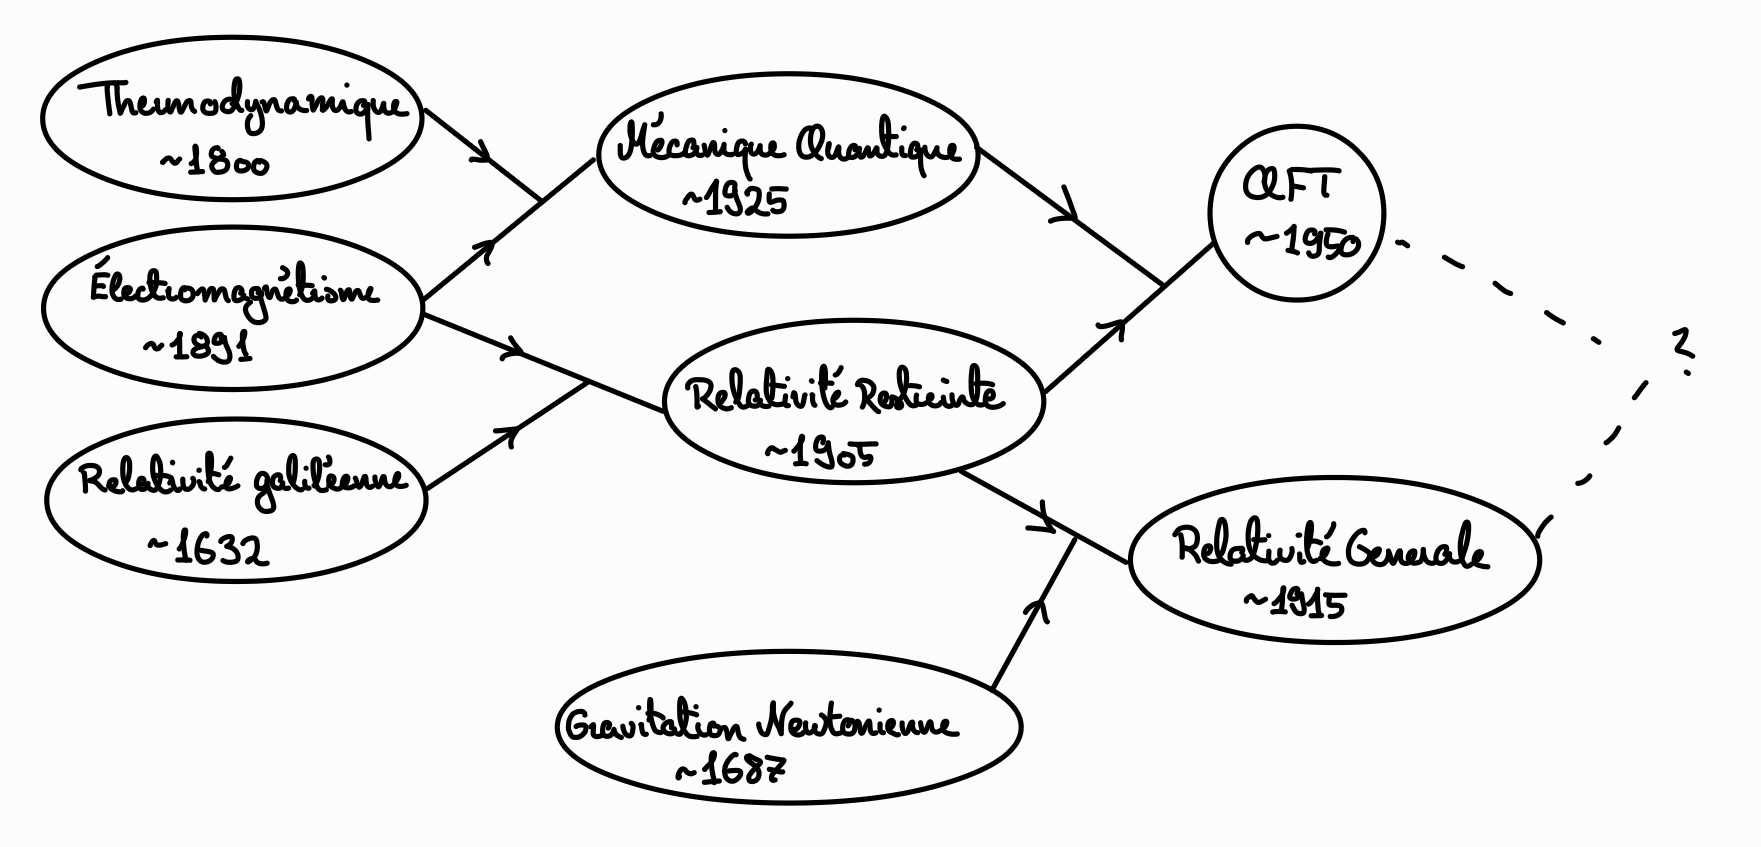
\includegraphics[scale=0.2]{Chapitres/1. Introduction/Images/Contradictions temp.png}
\end{center}
\begin{center}
    \textit{Contradictions equal progress.} (temp graph)
\end{center}
Il est intéressant de noter que la plupart des découvertes rappelées ci-dessus émergent plus d'\emph{expériences de pensée} plutôt que de réelles exprériences de laboratoire qui ont abouti à des révolutions. Einstein sera souvent guidées par celles-ci, comme il le fût pour la relativité restreinte, pour établir les principes de la relativité générale.
\begin{center}
    \textit{Je tiens pour vrai que la pensée pure est compétente pour comprendre le réel.}
    
    \noindent \emph{Ma conviction est que nous sommes en mesure, grâce à une construction purement mathématique, de trouver les concepts, ainsi que les lois qui les relient, propres à nous ouvrir les portes de la compréhension des phénomènes natures.}
\end{center}
\begin{flushright}
    - Albert Einstein
\end{flushright}
\subsection{L'incompatibilité de la relativité restreinte et la gravitation newtonienne}
Dans le cas de la relativité générale (RG), les théories qui ont poussées à sa création sont la relativité restreinte (RR) et la loi de gravitation universelle de Newton. Pour rappel, cette dernière stipule qu'un corps de masse $m$ soumis uniquement à l'attraction gravitationnelle d'un corps de masse $M$ subit une force
\begin{equation}
    \vect{F} = -G \, \frac{M m}{r^2}\,\vect{u}\indices{_r} \deq m\,\vect{g}\indices{_M}
\end{equation}
où $G$ est la constante de gravitation universelle, $r$ est la distance qui sépare les deux masses et $\vect{g}\indices{_M}$ le champ gravitationnel produit par la masse $M$.\\
Bien que cette théorie ait connu un immense succès pendant plus de deux siècles, elle présente plusieurs incompatibilités avec la relativité restreinte. En voici quelques-unes :

\begin{enumerate}
    \item \textbf{Propagation instantanée de la gravitation} \\
    Imaginons que le soleil disparaît à un moment donné. Selon la loi de gravitation newtonienne, la force gravitationelle s'annulera instantanément (comme $M=0$). Or, la relativité restreinte indique que aucune information ne peut se propager plus vite que la lumière, qui prend 8 minutes pour parvenir à la Terre. La vitesse de propagation de la force gravitationnelle serait donc $v = \infty > c$.\\
    
    \item \textbf{Non-invariance de Lorentz}\\
    La force de gravitation $\vect{F}$ est invariante sous transformations de Galilée 
    \begin{align}
        \begin{dcases}
            t' = t \\
            x' = x - vt\\
            y' = y\\
            z'=z
        \end{dcases}
    \end{align}
    car la quantité $r^2 = (\vect{x}_m - \vect{x}_M )^2 $ est conservée. Néanmoins, elle n'est pas invariante sous les transformations de Lorentz reliant deux observateurs inertiels :
    \begin{align}
        \begin{dcases}
            t' = \gamma(t - \frac{v}{c^2}x) \\
            x' = \gamma(x - vt)\\
            y' = y\\
            z'=z
        \end{dcases}
    \end{align}

    avec le facteur de Lorentz $\gamma = \dfrac{1}{\sqrt{1 - \frac{v^2}{c^2}}}$. \\
    
    \item \textbf{Non-linéarité d'une théorie relativiste de la gravitation}\\
    D'après la relativité restreinte, la masse est seulement une autre forme d'énergie. Ainsi, puisque la gravité couple à la masse (la masse est la \emph{charge gravitationnelle}), elle doit aussi coupler à l'énergie dans une théorie relativiste. Autrement dit, le contenu en énergie du système affecte le champ de gravitation. En particulier, la gravité devra coupler à l'énergie gravitationnelle, donc à elle-même. Les nouvelles équations du champ gravitationnel (\ref{eq:Einstein introduction}) seront intrinsèquement non-linéaires : le champ dû à la somme de deux masses n'égale pas la somme des champs gravitationnels des deux masses isolées, car l'énergie gravitationnelle d'interaction du système doit être pris en considération.\\
    
    Comparativement, l'équation de Poisson pour un potentiel gravitationnel newtonien s'écrit : 
    \begin{equation}
        \Delta \Phi = 4\pi \, G \,\rho
    \end{equation}
    où $\Phi$ est le potentiel gravitationnel (énergie) et $\rho$ est la masse volumique. En relativité restreinte, la densité $\rho$ devient alors dépendante de $\Phi$. On dit alors que la gravité est \emph{bouclée sur elle-même}. \\
 \end{enumerate}
 De plus, on peut se poser une question \emph{d'équivalence des référentiels} : en relativité galiléenne, il semble que les référentiels intertiels jouent un rôle privilégié : les lois de la physique y sont plus simples. Pourquoi une telle classe de référentiels existerait-elle ? De plus, il y a l'ambiguité du choix d'un premier référentiel intertiel, comme nous ne pouvons pas définir celui-ci de manière absolue. \\
 La relativité générale répond à ces questions en affirmant que \emph{tous} les référentiels sont équivalents pour la formulation des lois physiques, qu'ils soient inertiels ou non.

Avec ces ces inconsistence en tête, Einstein se lança dans la tâche d'incorporer l'interaction gravitationnelle en une théorie relativiste. Max Planck, ayant eu vent de l'entreprise d'Einstein lui aurait écrit :
\begin{center}
    \textit{As an older friend, I must advise you against it for, in the first place you will not succeed, and even if you succeed, no one will believe you.}
\end{center}
Et d'autre part :
\begin{center}
    \textit{When a serious scientist tells you something can be done, he's must likely to be right; But when he tells you it cannot be done, he's most likely to be wrong.}
\end{center}
Et il se fait qu'Einstein était têtu.
\subsection{Comparaison avec l'électromagnétisme}
La loi de gravitation newtonienne possède une forme remarquablement proche de la loi de Coulomb (électrostatique) :
\begin{align}
    \vect{F} = \frac{1}{4\pi \varepsilon_0} \frac{Q q}{r^2} \,\vect{u}\indices{_r} = q \,\vect{E}_q
\end{align}
Cette similarité soulève une question importante : pourquoi l'électromagnétisme ne souffre-t-il pas des mêmes problèmes que ceux évoqués pour la gravitation newtonienne ? La réponse réside simplement dans le fait que  la loi de Coulomb n'est qu'un cas particulier des équations de Maxwell qui, quant à elles, sont bien compatible avec la relativité restreinte. 
\begin{rap}
    Le quadri-potentiel électromagnétique $A^\mu = (\phi/c,\vect{A})$ s'écrit en fonction des champs $(\vect{E},\vect{B})$ selon :
    \begin{align}
        \begin{dcases}
            \vect{E} = - \vect{\nabla} \phi - \frac{\pd \vect{A}}{\pd t} \\
            \vect{B} = \vect{\nabla} \times \vect{A}
        \end{dcases}
    \end{align}
    Le champ électromagnétique peut donc être complètement décrit par les potentiels $(\vect{A},\phi)$. 
\end{rap}
\begin{rap}
    Le \emph{tenseur de Faraday} (également appelé le \emph{tenseur d'intensité du champ EM}) est un tenseur complètement anti-symmétrique donné par
    \begin{equation}
    \label{eq:Farady intro}
        F\indices{_\mu_\nu} \deq \pd_\mu A_\nu - \pd_\nu A_\mu
    \end{equation}
\end{rap}
\begin{exerc}
    Trouvez à partir de \ref{eq:Farady intro} la relation du tenseur de Faraday et les champs $(\vect{E},\vect{B})$.
\end{exerc}
\cutebreak
Armé de ces définitions, les équations de Maxwell peuvent être exprimées sous une forme tensorielle\footnote{Nous reviendrons sur cette formulation plus en détail dans la suite du cours. En particulier, la notation $[]$ sur les indices peut être ignorée pour le moment.} :
\begin{align}
    \begin{dcases}
        \pd\indices{_\mu} F\indices{^\mu^\nu} = J\indices{^\nu} \\
        \partial\indices{_[ _\alpha} F\indices{_\mu_\nu _]} = 0
    \end{dcases}
\end{align}
où $J^\mu = (c \rho,\vect{A})$ est le quadri-courant. Dans cette forme, les équations de Maxwell sont manifestement invariantes de Lorentz\footnote{Pour être tout à fait exact, il s'agit d'une covariance. De nouveau, nous y reviendrons plus tard.}.
\\
Vu qu'il s'agit d'équations tensorielles (pour des transformations de Lorentz), elles sont valables dans n'importe quel référentiel inertiel, et leur covariance est immédiate (voir ci-dessous).
\begin{itemize}
    \item \textbf{Loi de transformation de la force de Coulomb}\\
    À partir des équations de Maxwell, il est facile de montrer la force agissant sur une particule de charge $q$ se déplaçant à vitesse $\vect{v}$ dans des champs $(\vect{E},\vect{B})$ est donnée par la force de Lorentz :
    \begin{equation}
        \vect{F} = q\,  (\vect{E} + \vect{v} \times \vect{B})
    \end{equation}
    Nous verrons qu'en notation tensorielle, cette force s'écrit 
    \begin{equation}
        F^\alpha = q \, u_\beta F\indices{^\alpha ^\beta}
    \end{equation}
    où $u_\beta$ est la quadri-vitesse de la particule, et la force étant donné en fonction de la quadri-impulsion $P^\alpha = (\gamma m c, m \vect{v})$ selon :
    \begin{equation}
        F^\alpha \deq \frac{\td P\indices{^\alpha}}{\td \tau}
    \end{equation}
    où $\tau$ est le temps propre de la particule. La force de Coulomb étant un quadri-vecteur (et pas un scalaire), elle n'est \emph{pas} invariante sous transformation de Lorentz. Par contre, elle est \emph{covariante} : la connaissant dans un réfénrentiel de Lorentz (inertiel), on peut la connaître dans tout référentiel de Lorentz car elle obéit à une loi de transformation précise (ici $F^\alpha \to \Lambda\indices{^\alpha_\beta}F^\beta$).\\
    \item \textbf{Quid de la propagation instantanée ?}\footnote{Wald p.78}\\
    Un changement drastique se produit lorsqu'on passe de la théorie électrostatique de Coulomb aux équations de Maxwell : le champ électromagnétique $A_\mu = (\phi/c, - \vect{A})$ (avec $\vect{E} = - \vect{\nabla} \phi - \frac{\pd \vect{A}}{\pd t}$ et $\vect{B} = \vect{\nabla} \times \vect{A}$) devient une entité dynamique. En particulier, les équations de Maxwell dans le vide admettent des solutions ondulatoires, et la radiation électromagnétique peut se propager librement à la vitesse
    \begin{equation}
        v = c = \frac{1}{\sqrt{\varepsilon_0\mu_0}}
    \end{equation}
    dans le vide.
\end{itemize}
\begin{rmk}
    La théorie quantique des champs (QFT) nous indique de décrire les processus élémentaires en termes de particules élémentaires et de leurs collisions. En électrodynamique classique, ce sont les solutions ondulatoires des équations de Maxwell qui mènent le plus naturellement à une interprétation en termes de particules : le photon ($A_\mu$) se propageant à vitesse $c$. L'interaction n'est plus instantanée, et se fait via des perturbations du champ EM $A_\mu$ (qui se propagent à vitesse $c$), ou via échange de photons dans la théorie quantique.
\end{rmk}
\begin{rmk}
    Un changement similaire se propduira pour la gravitation en passant de Newton à la relativité générale. Cette dernière admet des solutions ondulatoires dans le vide (les \emph{ondes gravitationnelles}) se propageant à vitesse $c$ et sont également associées à une particules : le \emph{graviton}.
\end{rmk}
La loi de Coulomb a donc l'avantage de dériver d'un cadre plus fondamental, dans lequel les problèmes liées à la propagation et à l'invariance sont résolues. En gravitation, notre objectif sera de construire une théorie similaire, cohérente avec la relativité restreinte. Dans cette théorie, la gravitation newtonienne ne sera qu'une approximation valable dans un régime particulier.

\section{Principe d'équivalence}
La théorie de gravitation d'Einstein repose en grande partie sur une idée conceptuellement simple, appelée le \emph{principe d'équivalence} (PE). Einstein lui-même la qualifia de \emph{l'idée la plus heureuse de sa vie}. Nous rencontrerons ce principe à plusieurs reprises. Dans cette introduction, nous en donnerons une version littéraire, avant d'attaquer des formulations plus mathématiques dans les chapitres suivants. Certaines références différencient plusieurs formulations du PE. Voici-en un bref apperçu :
\begin{itemize}
    \item \textbf{Le PE faible} \\
    Postule l'équivalence entre masse inertielle et masse gravitationnelle (discuté dans la section \ref{sec:PE1} qui suit).\\
    \item \textbf{Le PE d'Einstein}\\
     Forme principale du principe d'équivalence dans la relativité générale, que nous adopterons dans ce cours (voir section \ref{sec:PE2}).\\
    \item \textbf{Le PE fort} \\
    Modification subtile du PE d'Einstein, impliquant un couplage de la gravitation avec elle-même. Cette formulation ne sera pas discutée dans ce cours.
\end{itemize}
Dans la suite du cours, nous désignerons par \emph{principe d'équivalence} uniquement la formulation d'Einstein.
\subsection{Préliminaires}
\label{sec:PE1}
Avant d'attaquer la formulation explicite du PE, formulons les observation fondamentales suivantes, distinguant l'interaction gravitationnelle d'autres types d'interactions.

Avant d'introduire formellement le principe d'équivalence (PE), posons quelques observations fondamentales, vérifiées expérimentalement, qui distinguent l'interaction gravitationnelle des autres types d'interactions.
\begin{theoremframe}
    \begin{propri}
        \label{post:PE1}
        L'effet de la gravité est \textbf{universel}. Tous les corps sont affectés de la même manière par la gravité, indépendamment de leur masse, charge, composition, etc.
    \end{propri}
\end{theoremframe}
Cette universalité fut mise en évidence pour la première fois par Galilée, dans sa fameuse expérience de la chute des corps. Cette expérience est illustrée plus récemment par la mission \textsc{Apollo 15} en 1971.
\begin{theoremframe}
    \begin{propri}
        \label{post:PE2}
        La gravité est toujours attractive.
    \end{propri}
\end{theoremframe}
En particulier, la gravité ne peut pas être écrantée. Cela la distingue fondamentalement de l'électromagnétisme, où il existe des charges positives et négatives. Cet écrantage est illustrée en EM par la cage de Faraday.

\begin{rmk}
    La propriété \ref{post:PE1} implique\footnote{Ou plus précisément, une justification de cette propriété est} l'égalité entre la masse inertielle $m_i$ et la masse gravitationnelle $m_g$. La première apparaît dans la deuxième loi de Newton $\vect{F} =m_{i}\vect{a}$, alors que la seconde est définie par la loi de gravitation newtonienne $\vect{F} =m_{g}\vect{g}_\mathbf{M}$. En supposant que le corps est soumis uniquement à un champ gravitationnel, nous avons :
    \begin{equation}
        \vect{a} = \frac{m_g}{m_i} \, \vect{g}
    \end{equation}

    Expérimentalement, nous n'observons aucune différence entre ces deux paramètres, alors qu'a priori, ils n'ont aucun lien. D'après les dernières mesures (le satellite \textsc{Microscope}) :
    \begin{equation}
        \left| 1 - \frac{m_i}{m_g} \right| \lesssim 10^{-14}
    \end{equation}
    Tous les corps chutent avec la même accélération dans un champ gravitationnel, indépendamment de leur \emph{charge gravitationnelle} : $\vect{a} = \vect{g}$. En comparaison, l'interaction électromagnétique montre un comportement très différent :
    \begin{equation}
        \vect{F} = q \, \vect{ E} \iff \vect{a} = \frac{q}{m_i} \, \vect{E}
    \end{equation}
    qui dépend explicitement de $q$ et $m_i$.
\end{rmk}
\begin{rmk}
    Le postulat \ref{post:PE2} permet d'expliquer pourquoi l'interaction gravitationnelle est observable à des échelles macroscopiques malgré son extrême faiblesse :
    \begin{equation}
        \left| \frac{F_g}{F_e}\right| \sim 10^{-43}
        \label{force gravité}
    \end{equation}
    Contrairement, l'interaction EM n'a pas d'effets macroscopiquement importants, car ceux-ci s'estompent par écrantage (corps macroscopiquement neutres).
\end{rmk}
\begin{center}
        \textit{La gravité est partout et affecte tous les corps de la même façon.}
    \end{center}
\subsection{L'ascenseur d'Einstein}
Einstein eut l'intuition que l'équivalence entre masse inertielle et masse gravitationnelle, loin d'être une coïncidence, indiquait quelque chose de fondamental sur la nature de la gravitation : la gravité et l'inertie (ou l'accélération) seraient \emph{indistinguables}. Il illustra cette idée par la célèbre expérience de pensée suivante.

\subsubsection{Gravité et inertie}
Supposons qu'une personne se trouve dans une boite isolée de l'extérieur (disons, un ascenseur). Lorsqu'elle lâche un objet, celui-ci tombe vers le sol (disons, accéléré uniformément). Deux conclusions lui sont possible à partir de cette interprétation :
\begin{itemize}
    \item L'objet retombe sous l'effet d'un champ gravitationnel, alors que l'ascenseur est immobile.
    \item L'objet retombe par effet d'inertie : l'ascenseur accélère vers le haut alors que l'objet relâché reste immobile du point de vue d'un observateur extérieur. 
\end{itemize}
\begin{center}
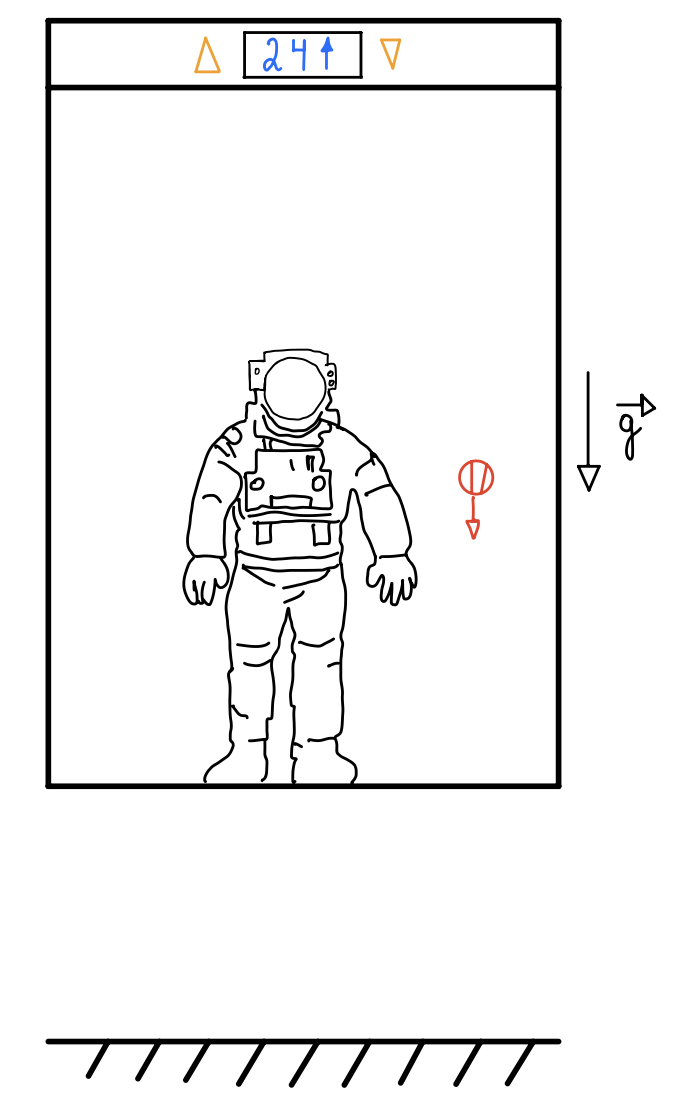
\includegraphics[scale=0.2]{Chapitres/1. Introduction/Images/homme ascenseur.png}
\includegraphics[scale=0.2]{Chapitres/1. Introduction/Images/homme fusée.png}
%\captionof{figure}{Plot de l'étude sur le HIV}
%\label{Plot_1}
\end{center}
Du point de vue de l'observateur à l'intérieur, confiné à une petite région de l'espace, la gravité et l'accélération uniforme sont indistinguables, qui est confinée dans une petite région. 

\subsubsection{Apesanteur et chute libre}
Supposons à présent que lorsque la personne lâche l'objet, celui-ci reste immobile (ne tombe pas) du point de vue de la personne. À nouveau, deux conclusions lui sont possibles :
\begin{itemize}
    \item L'ascenseur est situé dans l'espace, loin du champ de gravitation : il est en apesanteur. L’objet flotte simplement car il n'est soumis à aucune force. On dit qu'il suit une \emph{trajectoire libre}.
    \item L'ascenseur est en chute libre dans le champ de gravitation terrestre. Le poids effectif de la personne et de l'objet est nul ($\vect{P} = m(\vect{g} + \vect{a})$ mais en chute libre, $\vect{a} = - \vect{g}$ et donc $\vect{P} = 0$).
\end{itemize}
Dans les deux cas, l'objet flotte dans l'ascenseur. Les effets de la gravité peuvent donc être annulés \emph{localement} (à l'intérieur de l'ascenseur) en se plaçant dans un référentiel en chute libre, i.e. le référentiel de l'objet qui est soumis à cette force gravitationnelle.

\begin{center}
\includegraphics[scale=0.2]{Chapitres/1. Introduction/Images/homme fussée apesenteur.png}
\end{center}
\begin{rmk}
    Notons que jusqu'à présent, toutes ces observations restent valable dans la théorie Newtonienne. En effet, il est possible d'annuler localement la force de gravitation. Il suffit seulement de changer de référentiel pour se mettre dans un référentiel avec une accélération égale à la force de gravitation : étant donné $\ddot{x} = g$ :
    \begin{align}
        \xi(t,x) = x - g \frac{t^2}{2}
    \end{align}
    Qui est tel que $\ddot{\xi} = 0$.
\end{rmk}
\cutebreak
Dans ce référentiel \emph{en chute libre}, et puisque les effets de la gravité ont été annulés pour tout ce que contient l'ascenseur, ce sont les lois physiques habituelles en l'absence de gravité qui sont appliquables. Inversément, en connaissant les lois physiques en l'absence de gravité, on devrait pouvoir les déterminer en présence de gravité grâce à la transformation permettant de passer d'un référentiel en chute libre à un référentiel général.
\subsection{Les deux formulations du principe d'équivalence}
\label{sec:PE2}
\begin{theoremframe}
    \begin{propri}[Principe d'équivalence, première version]
        En tout point de l'espace-temps, il est possible de choisir un système de coordonnées tel que localement autour de ce point, les lois de la physique prennent la même forme qu'en l'absence de gravitation dans un référentiel inertiel.
    \end{propri}
\end{theoremframe}
Un tel référentiel, dit \emph{en chute libre}, est appelé un référentiel localement inertiel (RLI).
\begin{theoremframe}
    \begin{propri}[Principe d'équivalence, deuxième version]
        Localement, aucune expérience ne permet de distinguer un champ de gravitation et une accélération uniforme. 
    \end{propri}
\end{theoremframe}
Notons que la notion \emph{locale} utilisé ici peut se définir d'une manière mathématiquement précise, sur laquelle nous reviendrons plus tard. Pour le moment, il est seulement important de retenir que l'équivalence entre gravitation et accélération n'est valable que dans des régions suffisamment restreintes de l'espace-temps, sans quoi les inhomogénéités du champ gravitationnel feront que l'effet sur des \emph{particules-test} ou objets environnants sera différent d'un référentiel accéléré uniformément.
% Image cf notes
En conclusion, l'impossibilité de distinguer localement les effets d'un champ de gravitation d'une accélération uniforme est un phénomène de la relativité générale analogue à l'impossibilité en relativité galiléenne de mesurer la vitesse absolue d'un observateur.

\subsection{Conséquence : le redshift gravitationnel}
Une célèbre prédiction du PE est le \emph{redshift gravitationnel}, c’est-à-dire une modification de la fréquence d’un signal lumineux lorsqu’il traverse un champ gravitationnel.
\subsubsection{2.4.1 Accélération uniforme et effet Doppler}
Considérons deux fusées séparées d'une distance $z$ et ayant une accélération relative uniforme $\vect{a}$. À l'instant $t_0=0$, un photon est émis par la fusée 1, qui, à cet instant, se déplace à une vitesse $v$. On souhaite calculer le redshift (par effet Doppler) qu'aura le signal quand il arrivera à la fusée 2 au temps $t_0 + t^*$. Comme l'accélération est constante, on a :
\begin{align}
    z(t) = z_0 + vt + \frac{at^2}{2}
\end{align}
En supposant que $v \ll c$, un rapide calcul montre que $t^* = z(t^*)/c$ (exercice d'échauffement). En $t_0+t^*$, la vitesse de la fusée réceptrice est 
\begin{equation}
    v+at^*=v+\frac{az}{c}.
\end{equation}

\begin{center}
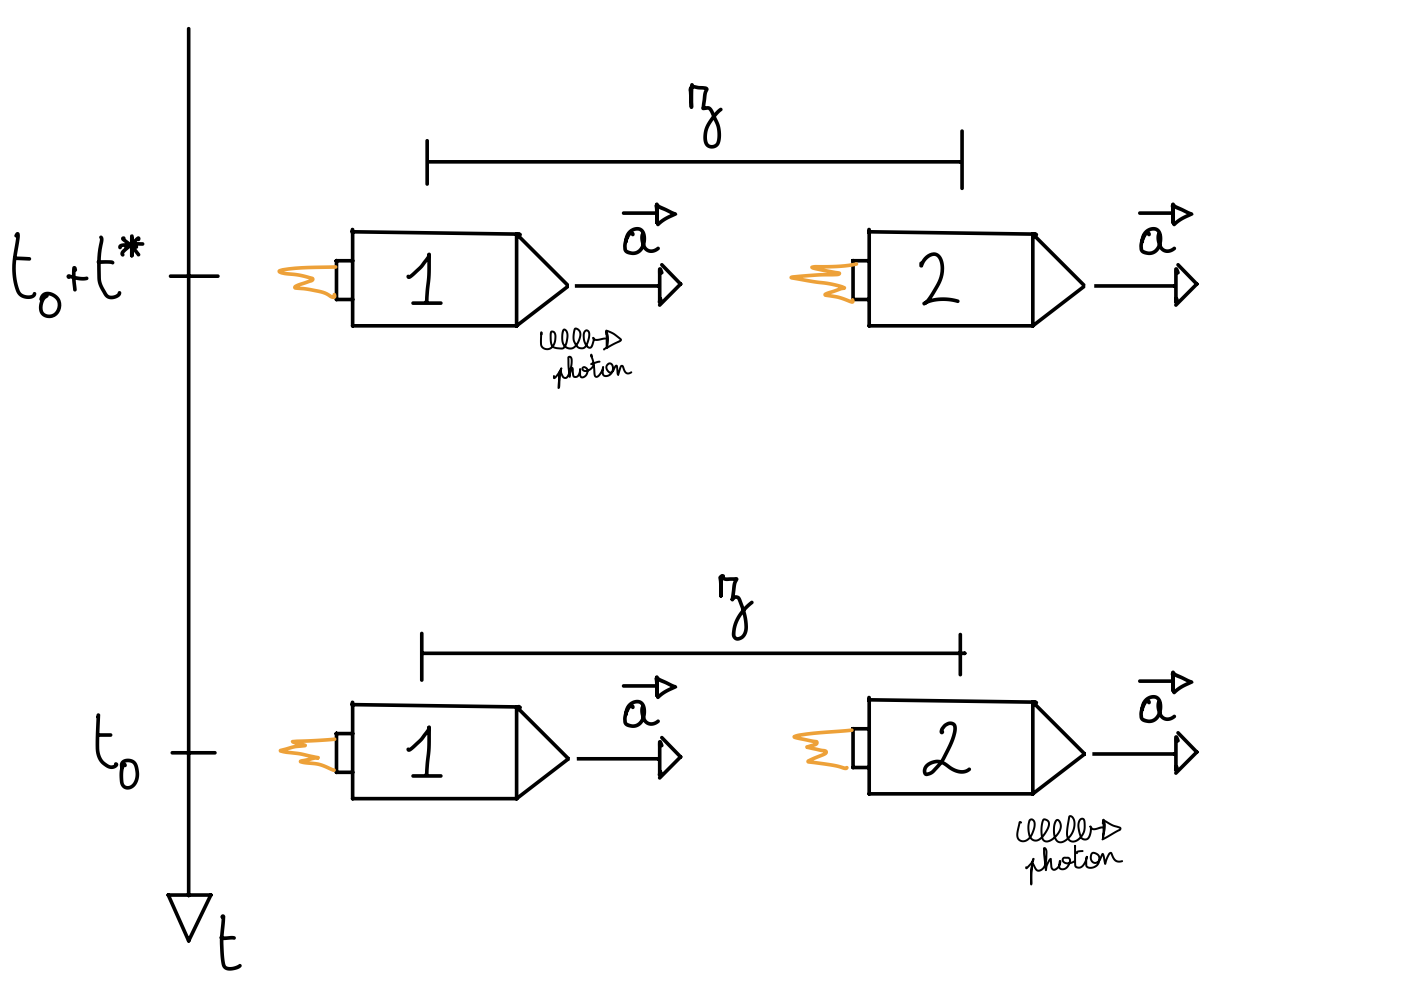
\includegraphics[scale=0.3]{Chapitres/1. Introduction/Images/photon.png}
\end{center}
L'émetteur et le récepteur n'ayant pas la même vitesse, la fréquence perçue par le récepteur va être modifié par effet Doppler :
\begin{align}
    \frac{\Delta\lambda}{\lambda_1}& = \frac{\lambda_2 - \lambda_1}{\lambda_1} = \frac{\Delta v}{c} = \frac{az}{c^2} \\
    &= \frac{\Delta T}{T_1} =\frac{\Delta \tau_2 - \Delta \tau_1}{\Delta \tau_1}
\end{align}
Comme $\delta v > 0$ on aura $\Delta \tau_2 > \Delta \tau_1$. En imaginant que le signal envoyé correspond à l'horloge interne de la fusée 1, on conclut que \emph{le temps s'écoule plus vite pour la fusée 2} . 

\subsubsection{2.4.2 Champ gravitationnel et effet Doppler}
En vertu du PE, la même phénomène doit se produire dans un champ de gravitation uniforme $g$. Supposons qu'une personne se trouve en haut d'une tour à hauteur $z_2$ et une deuxième personne en bas de la tour à une hauteur $z_1$ envoie un signal $\lambda_1$ vers la personne en haut de la tour. 

\begin{center}
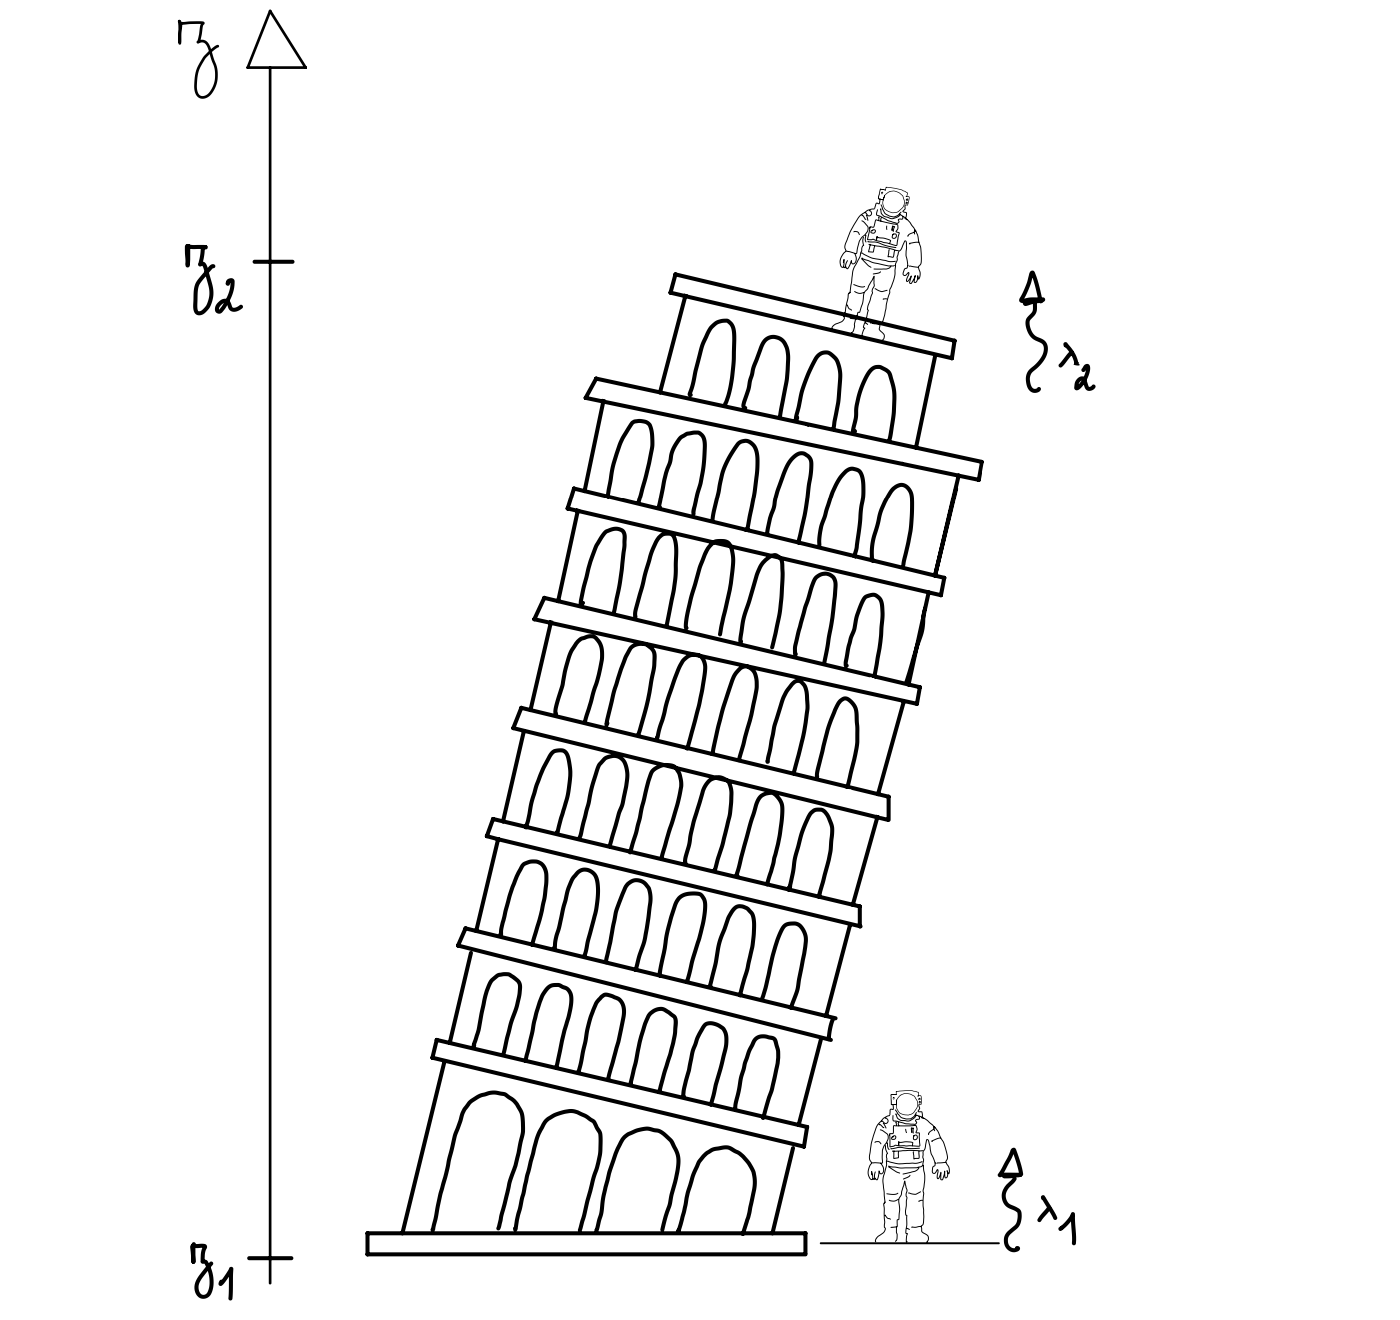
\includegraphics[scale=0.3]{Chapitres/1. Introduction/Images/Tour.png}
\end{center}
Comme les deux situations sont indistinguables, on doit trouver :
\begin{equation}
    \frac{\Delta \lambda}{\lambda} = \frac{\Delta T}{T} = \frac{g(z_2 - z_1)}{c^2}>0
\end{equation}
Et on trouvera donc que $T_2 > T_1$, c'est-à-dire que la période mesuré en haut de la tour sera plus grande que celle mesuré en bas de la tour. 

En conclusion, dans un champ de gravitation, la période du signal n'est pas la même au pied de la tour que en haut de la tour. Le temps s'écoule plus lentement le plus le champ de gravitation est fort\footnote{cf. \emph{Interstellar} lorsqu'iels se rapprochent du trou noir.}. Il s'agit d'un \textit{redshift gravitationnel}. 

\subsection{Remarque sur la nature géométrique de l'espace-temps en présence de gravitation}
Le redshift gravitationnel a une interprétation importante quant à la nature même de l'espace-temps. Supposons à présent qu'on envoie une onde périodique vers le haut de la tour, dont deux fronts d'onde sont séparés d'un temps $\Delta t_1 = \lambda_1/c$. Par contre, en haut de la tour, le signal reçu possède une période $\Delta t_2 = \lambda_2/c > \Delta t_1$, en vertu du redshift gravitationnel. Mais si le champ de gravitation est statique, c'est-à-dire indépendant du temps (ce qu'on a supposé implicitement jusqu'à ici), les chemins suivis dans l'espace-temps par les trains d'onde successifs A et B doivent être congruents (parallèles) quelle que soit la forme précise de ces chemins (que l'on ne prétend pas connaître en présence de gravitation). Alors, on devrait nécessairement avoir $\Delta t_1 = \Delta t_2$, mais ce n'est pas le cas ! \\
\\
Une interprétation est que l'espace-temps à travers lequel les photons se propagent est courbe. En effet, dans un espace plat (par exemple l'espace Euclidien $\R^3$), deux trajectoires initialement parallèles conservent leur séparation au cours du temps. En revanche, en présence de courbure, cette propriété n'est plus garantie. Par exemple, sur la sphère $S^2$, deux \emph{lignes} (géodésiques) initialement parallèles ne conservent pas la distance entre-eux, et finiront même par se croiser !

On ne peut pas à strictement parler \emph{prouver} que l'espace-temps est courbe (pas plus qu'on ne peut \emph{prouver} les lois de Newton). On peut par contre envisager l'hypothèse, d'en déduire des prédictions qui l'infirmeront ou la confirmeront. Nous allons donc être amenés à développer des outils permettant de décrire des espaces-temps courbes, mais qui localement \emph{ressemblent} à l'espace-temps plat de (Poincaré) Minkowski, puisque localement dans un référentiel approprié, la relativité restreinte doit y être applicable.

Imaginons à présent que le premier signal à période $T_0$ arrive en haut de la tour avec une période $T_0+T_1$. Que se passerait-il si un deuxième signal est renvoyé du bas de la tour avec une fréquence de $T_0+T_1$ ? En supposant une gravitation statique, il serait évident de conclure que la différence en fréquence $T_2 = T_1$. Néanmoins, cet argument n'est applicable que si l'espace-temps est plat. Nous verrons dans la suite que si $T_2 \neq T_1$, alors l'espace-temps est courbe.

\begin{center}
    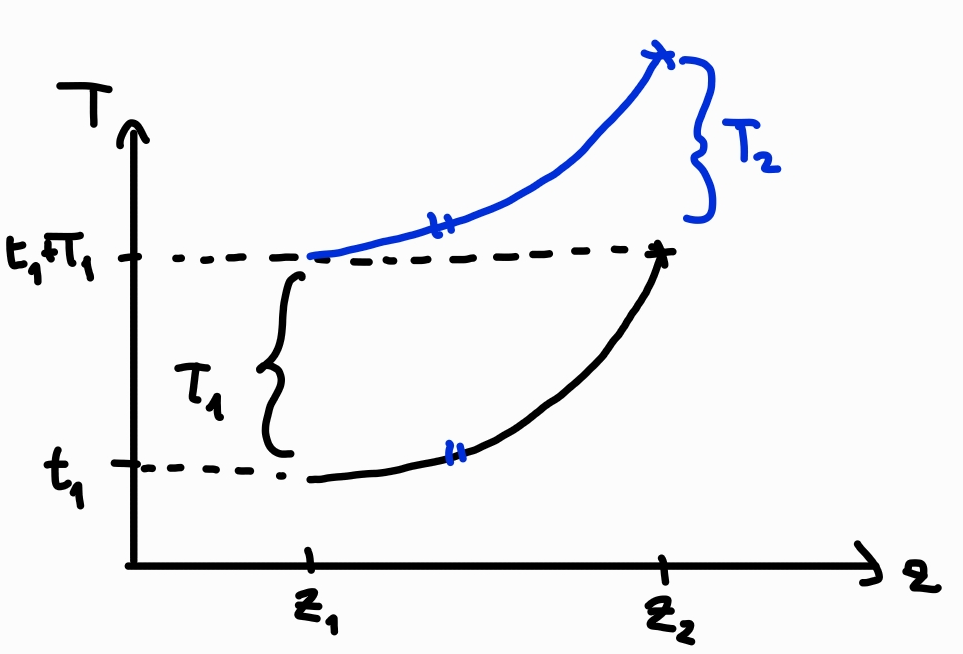
\includegraphics[scale=0.3]{Chapitres/1. Introduction/Images/confusion pure temp.png}
\end{center}
 %

\chapter{Rappels de Relativité Restreinte}
La première partie de ce chapitre (section 1-4) est constitué exclusivement de rappels de la relativité restreinte. Celle-ci sera importante dans la suite du cours, comme elle reste valable \emph{localement} en présence de gravitation, dans un RLI. La seconde partie du chapitre (section 5-6) approfondit ces notions via une étude de la \emph{structure causale} de l'espace de Minkowski.


\section{Postulats de la relativité restreinte}
En 1905, Einstein énonça les deux postulats de la relativité restreinte:
\begin{theoremframe}
    \begin{post}[Loi de la relativité]
        Les lois de la physique prennent la même forme dans tous les référentiels inertiels. Il est donc impossible de distinguer un référentiel inertiel d'un autre.
    \end{post}
\end{theoremframe}
\begin{theoremframe}
    \begin{post}[Universalité de la vitesse de la lumière]
        La vitesse de la lumière $c$ dans le vide est isotope et prend la même valeur dans tout référentiel inertiel.
    \end{post}
\end{theoremframe}
\section{Définition d'un référentiel inertiel}

La relativité restreinte est une théorie de l'espace-temps plat quadri-dimensionnel $\R ^{1,3}$, dont les points sont appelés des \emph{événements}. Les \emph{référentiels} permettent d'enregistrer ces événements, et sont constitués de:
\begin{enumerate}
    \item un repère spatial cartésien orthonormé au repos de coordonnées $(x, y, z) = \vect{x}$, souvent écrit en composantes $x^k$ où $k=1, 2, 3$. 
    \item des horloges qui déterminent quand l'événement a lieu $x^0 = ct$. \\
\end{enumerate}
Un point $x^\mu\in \R^{1,3}$ dans ce repère avec $\mu=0,1,2,3$ est appelé un quadri-vecteur (ou 4-vecteur), et possède des unités de longueur $[x^\mu ] = L$. Naturellement, les événements existent indépendamment des référentiel, tout comme les points du plan euclidien existent indépendamment des repères cartésiens (ce sont des points physiques).
\begin{theoremframe}
\begin{rap}[Principe d'inertie]
    En l'absence de force appliquée, un corps se meut en mouvement rectiligne uniforme ou reste au repos.    
\end{rap}
\end{theoremframe}
\begin{theoremframe}
\begin{defi}
Un \emph{référentiel inertiel} est une référentiel dans lequel le principe d'inertie est vrai. 
\end{defi}
\end{theoremframe}
Étant donné un référentiel inertiel $O$, le principe d'inertie ne peut trivialement pas être vérifié dans des repères accélérés par rapport à $O$. 

\begin{exmp}
    \textbf{Un référentiel non-inertiel} :\\
    Un carrousel qui tourne sur lui-même. Dans celui-ci, si une personne lance une balle à une personne en face de lui lorsque le carrousel est au repos la balle suit une trajectoire en ligne droite (le principe d'inertie est donc respecté). Quand le carrousel commence à tourner, la personne n'arrivera pas a attraper la balle car elle n'aura pas un mouvement rectiligne (le principe d'inertie n'est pas respecté donc on n'est pas dans un référentiel inertiel).
\end{exmp}


\section{Intervalle d'espace-temps}

L'intervalle (relativiste) est la contrepartie pour l'espace-temps plat $\R^{1,3}$ de la distance pour un espace euclidien.

\begin{theoremframe}
    \begin{defi}
        Soient deux événements $P,Q$ à coordonnées $x_P^\mu, x_Q^\mu$ dans un référentiel inertiel donné. L'\emph{intervalle} d'espace-temps plat entre $P$ et $Q$ est donné par
        \begin{align}
            (\Delta s)^2 &\equiv -(c\Delta t)^2 + (\Delta x)^2 + (\Delta y)^2 + (\Delta z)^2\\
            &= \eta _{\mu \nu} \, \Delta x^{\mu} \Delta x^{\nu}
        \end{align}
        où $\Delta x^{\mu}=x^\mu_Q-x^\mu_P$ est la séparation entre les deux événements et où $\eta _{\mu \nu} \equiv \textrm{diag}(-1, 1, 1, 1)$ est la métrique de Minkowski\footnote{Contrairement à la QFT, nous utiliserons dans l'ensemble de ce cours la convention \emph{mostly positive} de la métrique de Minkowski, comme il est d'usage en RG et cosmologie.}. La sommation est sous-entendue sur les indices répétés.
    \end{defi}
\end{theoremframe}
Nous verrons que l'intervalle est préservé par les transformations de Poincaré propre octocrone $\ISO (3,1)^\uparrow$. L'intervalle définit une pseudo-métrique (au sens mathématique) sur $\R^{1,3}$ : contrairement à une métrique usuelle, elle n'est pas définie positive, et 
\begin{equation}
    \Delta s(x^\mu,y^\mu)=0 \centernot \implies x^\mu=y^\mu
\end{equation}

L'intervalle permet de construire une structure causale sur $\R^{1,3}$: les deux évènements $P$ et $Q$ ont un lien causal si et seulement si $(\Delta s)^2 < 0$. En effet, supposons par l'absurde que leur intervalle soit positif :

\begin{align}
    (\Delta s)^2 > 0 &\implies -(c\Delta t)^2 + (\Delta \vect{x})^2 > 0\\
    &\implies c^2 < \lt \frac{\Delta \vect{x}}{\Delta t} \rt^2 \equiv v^2\\
\end{align}

Mais comme aucune information ne peut propager plus vite que la vitesse,on conclut que les deux évènements ne sont pas causalement liés. 

\begin{theoremframe}
    \begin{propri}
        L'intervalle relativiste est invariant sous changement de référentiel inertiel.
    \end{propri}
\end{theoremframe}
\begin{proof}
Soient deux événements $P,Q \in \R^{1,3}$ séparés dans un référentiel inertiel $O$ par des coordonnées $\Delta x^{\mu}$ et dans un référentiel inertiel $O'$ par des coordonnées $\Delta x'^{\mu}$ .

    \begin{center}
        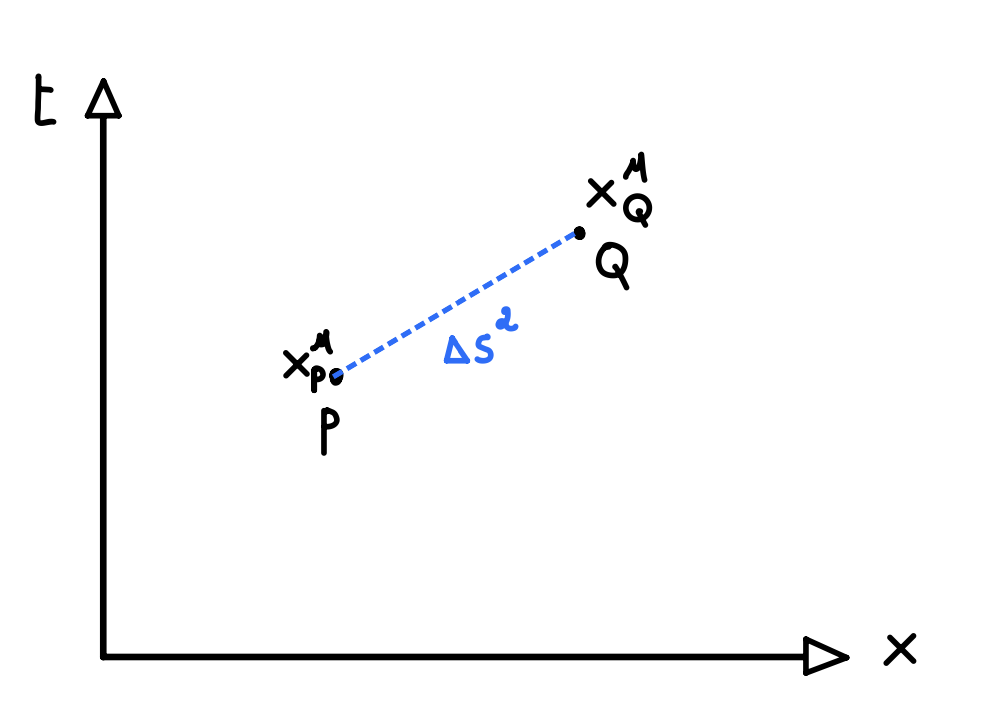
\includegraphics[scale=0.3]{Chapitres/2. Relativité Restreinte/Images/intervalle graph.png}
    \end{center}
    \begin{enumerate}
        \item Supposons qu'un signal lumineux joigne $P$ à $Q$. On a donc $\lt \dfrac{\Delta \vect{x}}{\Delta t} \rt^2 = v^2 = c^2$. Calculons $(\Delta s )^2$:
        \begin{align}
            (\Delta s )^2  & = -(c\Delta t)^2 + (\Delta \vect{x})^2\\
            \lt\frac{\Delta s}{\Delta t}\rt^2 & = -c^2 + \lt \frac{\Delta \vect{x}}{\Delta t} \rt^2\\
            & =0
        \end{align}
        Ainsi, $\Delta s = 0$. Dans le référentiel $O'$, on aura également $\Delta s' = 0$  car la vitesse de la lumière est la même dans tout les référentiel inertiel.
        \begin{equation}
            \lt \frac{\Delta s'}{\Delta t'} \rt^2 = -c^2 + v'^2 = 0
        \end{equation}
        Il en découle que si l'intervalle s'annule dans un référentiel inertiel, il s'annule dans tout référentiel inertiel. \\
        \item Montrons maintenant que peu importe valeur de $\Delta s$, on a que $\Delta s = \Delta s' $ pour tous référentiels inertiels.

        Comme les deux référentiels sont inertiels, ils sont reliés par une transformation linéaire: 
        \begin{equation}
            x'^{\mu} = \Lambda\indices{^\mu_\alpha} \, x^{\alpha} + a^{\mu}
            \label{def:poincaré}
        \end{equation}
        où $a\in \R^{1,3}$ est un constante et $\Lambda$ une matrice inversible. Les différences sont alors:
        \begin{equation}
            \label{eq:intervalle1}
            \Delta x'^{\mu} = \Lambda\indices{^{\mu}_{\alpha}} \,  \Delta x^{\alpha}
        \end{equation}
        et donc l'intervalle dans les deux référentiels s'écrit : 
        \begin{align}
            \label{eq:intervalle2}
            (\Delta s)^2 & = \eta _{\mu \nu} \, \Delta x^{\mu} \Delta x^{\nu}\\
            \label{eq:intervalle3}
            (\Delta s')^2 & = \eta _{\mu \nu} \, \Delta x'^{\mu} \Delta x'^{\nu}.
        \end{align}
        Autrement dit, $(\Delta s)^2$ et $(\Delta s')^2$ sont des polynômes du second degré en les $\Delta x^{\mu}$, car d'après \ref{def:poincaré}, $x'^\mu$ dépend linéairement de $x^\mu$. On a montré précédemment que si $(\Delta s)^2 = 0$ alors $(\Delta s')^2 = 0$ : les deux polynômes ont donc les mêmes racines. Or, deux polynômes du second degré qui ont les mêmes racines sont proportionnelles, c'est-à-dire qu'il existe $\kappa\in \R$ tel que
        \begin{equation} 
            \label{eq:intervalle4}
            (\Delta s)^2 = \kappa (\Delta s')^2.
        \end{equation}
        L'espace-temps est isotrope, et $\kappa$ ne peut donc que dépendre de la norme de la vitesse relative entre les deux référentiels : $\kappa(\vect{v})=\kappa(\lVert \vect{v} \rVert)$\footnote{Etant une propriété des deux référentiels, $\kappa$ ne peut que dépendre $\vect{v}$. Nous invitons le lecteur à argumenter pourquoi celui-ci ne peut pas dépendre des coordonnées d'espace.}. En particulier, on trouve $\kappa(\Vec{v}) = \kappa(-\vect{v})$. En effectuant le changement de référentiel inverse, on trouve que
        \begin{equation}
            (\Delta s')^2 = \kappa(-\vect{v}) (\Delta s)^2
            \label{eq:intervalle5}
        \end{equation}
        En combinant\ref{eq:intervalle4} avec \ref{eq:intervalle5}, on obtient finalement
        \begin{align}
            (\Delta s)^2 &= \kappa(\vect{v}) \kappa(-\vect{v}) (\Delta s)^2\\
            &= \kappa^2(\Delta s)^2
        \end{align}
        Il vient que $\kappa ^2= 1$ soit $\kappa = \pm 1$. En injectant \ref{eq:intervalle1} dans \ref{eq:intervalle3}, puis en utilisant la relation \ref{eq:intervalle4}, on trouve que
        \begin{equation}
            \eta_{\mu\nu} \, \Delta x^\mu \Delta x^\nu = \kappa \, \eta_{\alpha\beta} \, \Lambda\indices{^\alpha_{\mu}} \, \Lambda\indices{^\beta_{\nu}}\, \Delta x^\mu \Delta x^\nu
        \end{equation}
        soit (en notation matricielle) :
        \begin{equation}
            \label{eq:Lorentz pre}
            \eta = \kappa \,\eta'=\kappa \,\Lambda^T\eta \Lambda
        \end{equation}
        Comme $\eta$ est une forme quadratique symétrique et $\eta'$ est un changement de base de $\eta$ ($\Lambda$ est inversible), le \textit{théorème de Sylvester}\footnote{c.f. votre cours d'algèbre de BA1.} impose que la signature de $\eta'$ ne change pas, et donc que $\kappa=1$.

        On peut ainsi conclure que $(\Delta s')^2 = (\Delta s)^2$.
    \end{enumerate}
\end{proof}

\section{Transformations de Lorentz et de Poincaré}

On définit les transformations de Poincaré comme l'ensemble des isométries sur l'espace-temps munie de la (pseudo-)métrique de Minkowski $(\R^{1,3},s)$, c'est-à-dire les transformations qui relient des référentiels inertiels et telles que la vitesse de la lumière $c$ soit conservée.

Soient deux référentiels inertiels $O$ et $O'$ qui ont respectivement comme coordonnées $x^{\alpha}$ et $x^{\alpha '}$. 
Comme les deux référentiels sont inertiels ils doivent être reliés par la transformation \ref{def:poincaré}. 

Comme vu dans la section précédente, en prenant $\kappa = 1$ dans la relation \ref{eq:Lorentz pre}, on trouve que

\begin{equation}
    \label{eq:Lorentz}
    \boxed{\Lambda ^{T} \eta \Lambda = \eta}
\end{equation}

L'ensemble des matrices satisfaisant à l'équation \ref{eq:Lorentz} est appelé le \textit{groupe de Lorentz} O$(3,1)$. L'ensemble des couples $(\Lambda,a)$ satisfaisant à \ref{eq:intervalle1} et donc à \ref{eq:Lorentz} est appelé \textit{groupe de Lorentz inhomogène} ou le \textit{groupe de Poincaré} $IO(3,1)$. 

\begin{rmk}
Lorsque $\eta = \text{diag}(-1,...,-1,1,...,1)$ avec $p$ fois -1 et $q$ fois +1, on appelle le groupe vérifiant \ref{eq:Lorentz} IO$(p,q)$
    
\end{rmk}
\begin{rmk}
    Dans le cas particulier $p =0$ et $q=3$, on a le groupe IO(3) c'est-à-dire avec $\Lambda ^{T} \Lambda = I_{3x3}$. 
\end{rmk}

Les transformations telles que $\Lambda =  I$ appartiennent au groupe de translation.

\subsection{Groupe de Lorentz}

Le groupe de Lorentz O(3,1) possède deux sous-groupes non-triviaux. En particulier, il possède quatre composantes non-connexes.

\begin{enumerate}
    \item En reprenant la relation $\Lambda ^{T} \eta \Lambda = \eta$, et calculant le déterminant:
    \begin{equation}
        \det \Lambda^{T} \det \eta \det\Lambda = \det \eta \\
        \implies \det\Lambda = \pm 1
    \end{equation}
    Comme il est impossible de passer continûment d'un élément de $\det =1$ à un élément de $\det = -1$, le groupe possède deux composantes non-connexes. On note O$(3,1)_\pm$ la partie du groupe de Lorentz à $\det = \pm 1$.\\
    \\
    Uniquement la composante O$(3,1)_+$ est un sous-groupe de O(3,1), appelé groupe spécial de Lorentz noté SO$(3,1)$\footnote{En effet, c'est la seule des deux composantes qui inclut l'élément identité.}. \\

    
    \item Réécrivons la relation de définition \ref{eq:Lorentz} du groupe de Lorentz. En composantes, on trouve
    \begin{equation}
        \eta_{\alpha \beta}\, \Lambda\indices{^\alpha_{\mu}} \,\Lambda\indices{^\beta_{\nu}} = \eta_{\mu \nu}
    \end{equation}
    Ainsi, pour la composante $\mu = \nu =0$:
    \begin{align}
        \eta_{0 0} &= \eta_{\alpha \beta} \,\Lambda\indices{^\alpha_{0}} \, \Lambda\indices{^\beta_{0}} \\
        \implies -1 &= -(\Lambda\indices{^0_{0}})^2 + \sum_{k}(\Lambda\indices{^k_0})^2\\
        \implies (\Lambda\indices{^0_0})^2 &= 1 + \sum_{k}(\Lambda\indices{^k_0})^2\\
        \implies (\Lambda\indices{^0_0})^2 &\geq 1
    \end{align}
    On trouve donc de nouveau deux composantes non connexes notées O(3,1)$^\uparrow$ (si $\Lambda\indices{^0_0} \geq 1$) et O(3,1)$^\downarrow$ (si $\Lambda\indices{^0_0} \leq - 1$). Uniquement O(3,1)$^\uparrow$ est un sous-groupe de O(3,1) et est aussi appelé le sous-groupe orthochrone de Lorentz.
\end{enumerate}
Le groupe O(3,1)$^\uparrow_+ \equiv$ SO(3,1)$^\uparrow$ est un sous-groupe normal de O(3,1). Nous renvoyons vers votre cours de théorie des groupes pour une étude détaillée du groupe de Lorentz.
\subsection{Exemple de transformation de Lorentz:}

\begin{exmp}
    Une rotation autour de l'axe $z$ peut être décrite par la matrice
    \begin{equation}
        \Lambda = \begin{pmatrix}
1 & 0 & 0 & 0\\
0 & \cos{\theta} & \sin{\theta} & 0\\
0 & -\sin{\theta} & \cos{\theta} & 0\\
0 & 0 & 0 & 1\\
\end{pmatrix}
    \end{equation}
    En notant $x'=\Lambda x$, on peut réécrire cette transformation comme
    \begin{align}
    \left\{
\begin{array}{l}
  t' =t \\
  x' = x\cos{\theta} + y\sin{\theta}\\
  y' = -x\sin{\theta} + y\cos{\theta}\\
  z' = z
\end{array}
\right.
\end{align}
Correspondant bien à une rotation autour de $z$.
\end{exmp}


\begin{exmp}
    Un \textit{boost} dans la direction $x$ peut être décrite par la matrice
    \begin{equation}
        \Lambda = \begin{pmatrix}
\cosh{\phi}& -\sinh{\phi} & 0 & 0\\
-\sinh{\phi} & \cosh{\phi} & 0 & 0\\
0 & 0 & 1 & 0\\
0 & 0 & 0 & 1\\
\end{pmatrix}
    \end{equation}
    De nouveau, on peut réécrire cette transformation comme 
\begin{align}
\label{eq:4.2.1}
    \left\{
\begin{array}{l}
  t' = \cosh{\phi}t - \sinh{\phi}x \\
  x' = -\sinh{\phi}t + \cosh{\phi}x\\
  y' = y\\
  z' = z
\end{array}
\right.
\end{align}
\end{exmp}
Pour montrer que cette transformation correspond bien à un boost dans la direction $x$, nous allons effectuer un changement de variable qui nous ramène aux transformations de Lorentz sous leur forme usuelle.

Posons $-1 < v\deq\tanh\phi < 1$ . Définissons de plus $\gamma \deq \cosh\phi$. Alors, $\sinh\phi = v \gamma$ et la transformation \ref{eq:4.2.1} se réécris comme
\begin{align}
\left\{
\begin{array}{l}
  t' = \gamma(t - vx) \\
  x' = \gamma(x - vt)\\
  y' = y \\
  z' = z
\end{array}
\right.
\end{align}
On peut également montrer que $\gamma$ correspond au facteur de Lorentz usuel:
\begin{align}
    \cosh^2{\phi} - \sinh^2{\phi} = 1\\
    \implies  1 - \tanh{\phi}^2 = \frac{1}{\cosh^2{\phi}}
\intertext{Donc}
    1 - v^2 = \frac{1}{\cosh^2{\phi}}
\intertext{Soit}
    \gamma = \sqrt{\frac{1}{1-v^2}} = \cosh{\phi}
\end{align}

\section{Structure causale de l'espace-temps de Minkowski}

\subsection{Le cône de lumière}
On introduit la notion de cône de lumière. 
\begin{theoremframe}
    \begin{defi}
        Soit $P \in \mathcal{M} = \R^{1, 3} = \mathcal{M}^{1, 3}$. Le \textit{cône de lumière} de $P$, noté $C_P$ est l'ensemble des points à distance nulle de $P$.
        \begin{equation}
            C_P = \ltc Q \in \mathcal{M} \mid \Delta s_{PQ} = 0\rtc
        \end{equation}

    \end{defi}
\end{theoremframe}
On se rappelle que l'intervalle d'espace-temps peut se réécrire comme:
\begin{equation}
    (\Delta s)^2 = -(\Delta t)^2 + \sum_{i}(\Delta x^{i})^2
\end{equation}
Le faite que $(\Delta s)^2 = 0$ implique donc que $\Delta t =
\sqrt{(\Delta x)^2 + (\Delta y)^2 + (\Delta z)^2}$, qui est la contrainte d'un 4-cône (à tout temps $\Delta t$ fixe, il s'agit d'une sphère de rayon $\Delta t$).

\begin{theoremframe}
    \begin{notat}
        Le cône de lumière va diviser l'espace de Minkowski en 3 régions tel que:
        \begin{enumerate}
            \item[\cRM{1}.] \textit{Le futur absolu} de $P$ correspond au cône de lumière supérieur rempli noté $C_{P}^{+}$.
            \item[\cRM{2}.] \textit{Le passé absolu} de $P$ correspond au cône de lumière inférieur rempli noté $C_{P}^{-}$. 
            \item[\cRM{3}.] \textit{L'ailleurs absolu} de $P$ correspond au complémentaire de $C_P^\pm $.
        \end{enumerate}
    \end{notat}
\end{theoremframe}
Ces trois régions sont illustrés sur la figure \ref{fig:2.1}. Justifions cette terminologie. Soient $P,Q\in \R^{1,3}$.

\begin{theoremframe}
    \begin{propri}
         Si $Q \in C_P^+$ (resp. $C_P^-$), alors $Q$ se produit après (resp. avant) $P$ pour tout référentiel inertiel.
    \end{propri}
\end{theoremframe}
\begin{proof}
    Exercice.
\end{proof}
La causalité est importante dans une théorie physique. Cette propriété assure que la causalité de deux évènements causalement connectés (ils se trouvent dans le cône de lumière de l'autre) est conservée pour tout référentiel inertiel. 
    \begin{figure}[H]
     \centering
        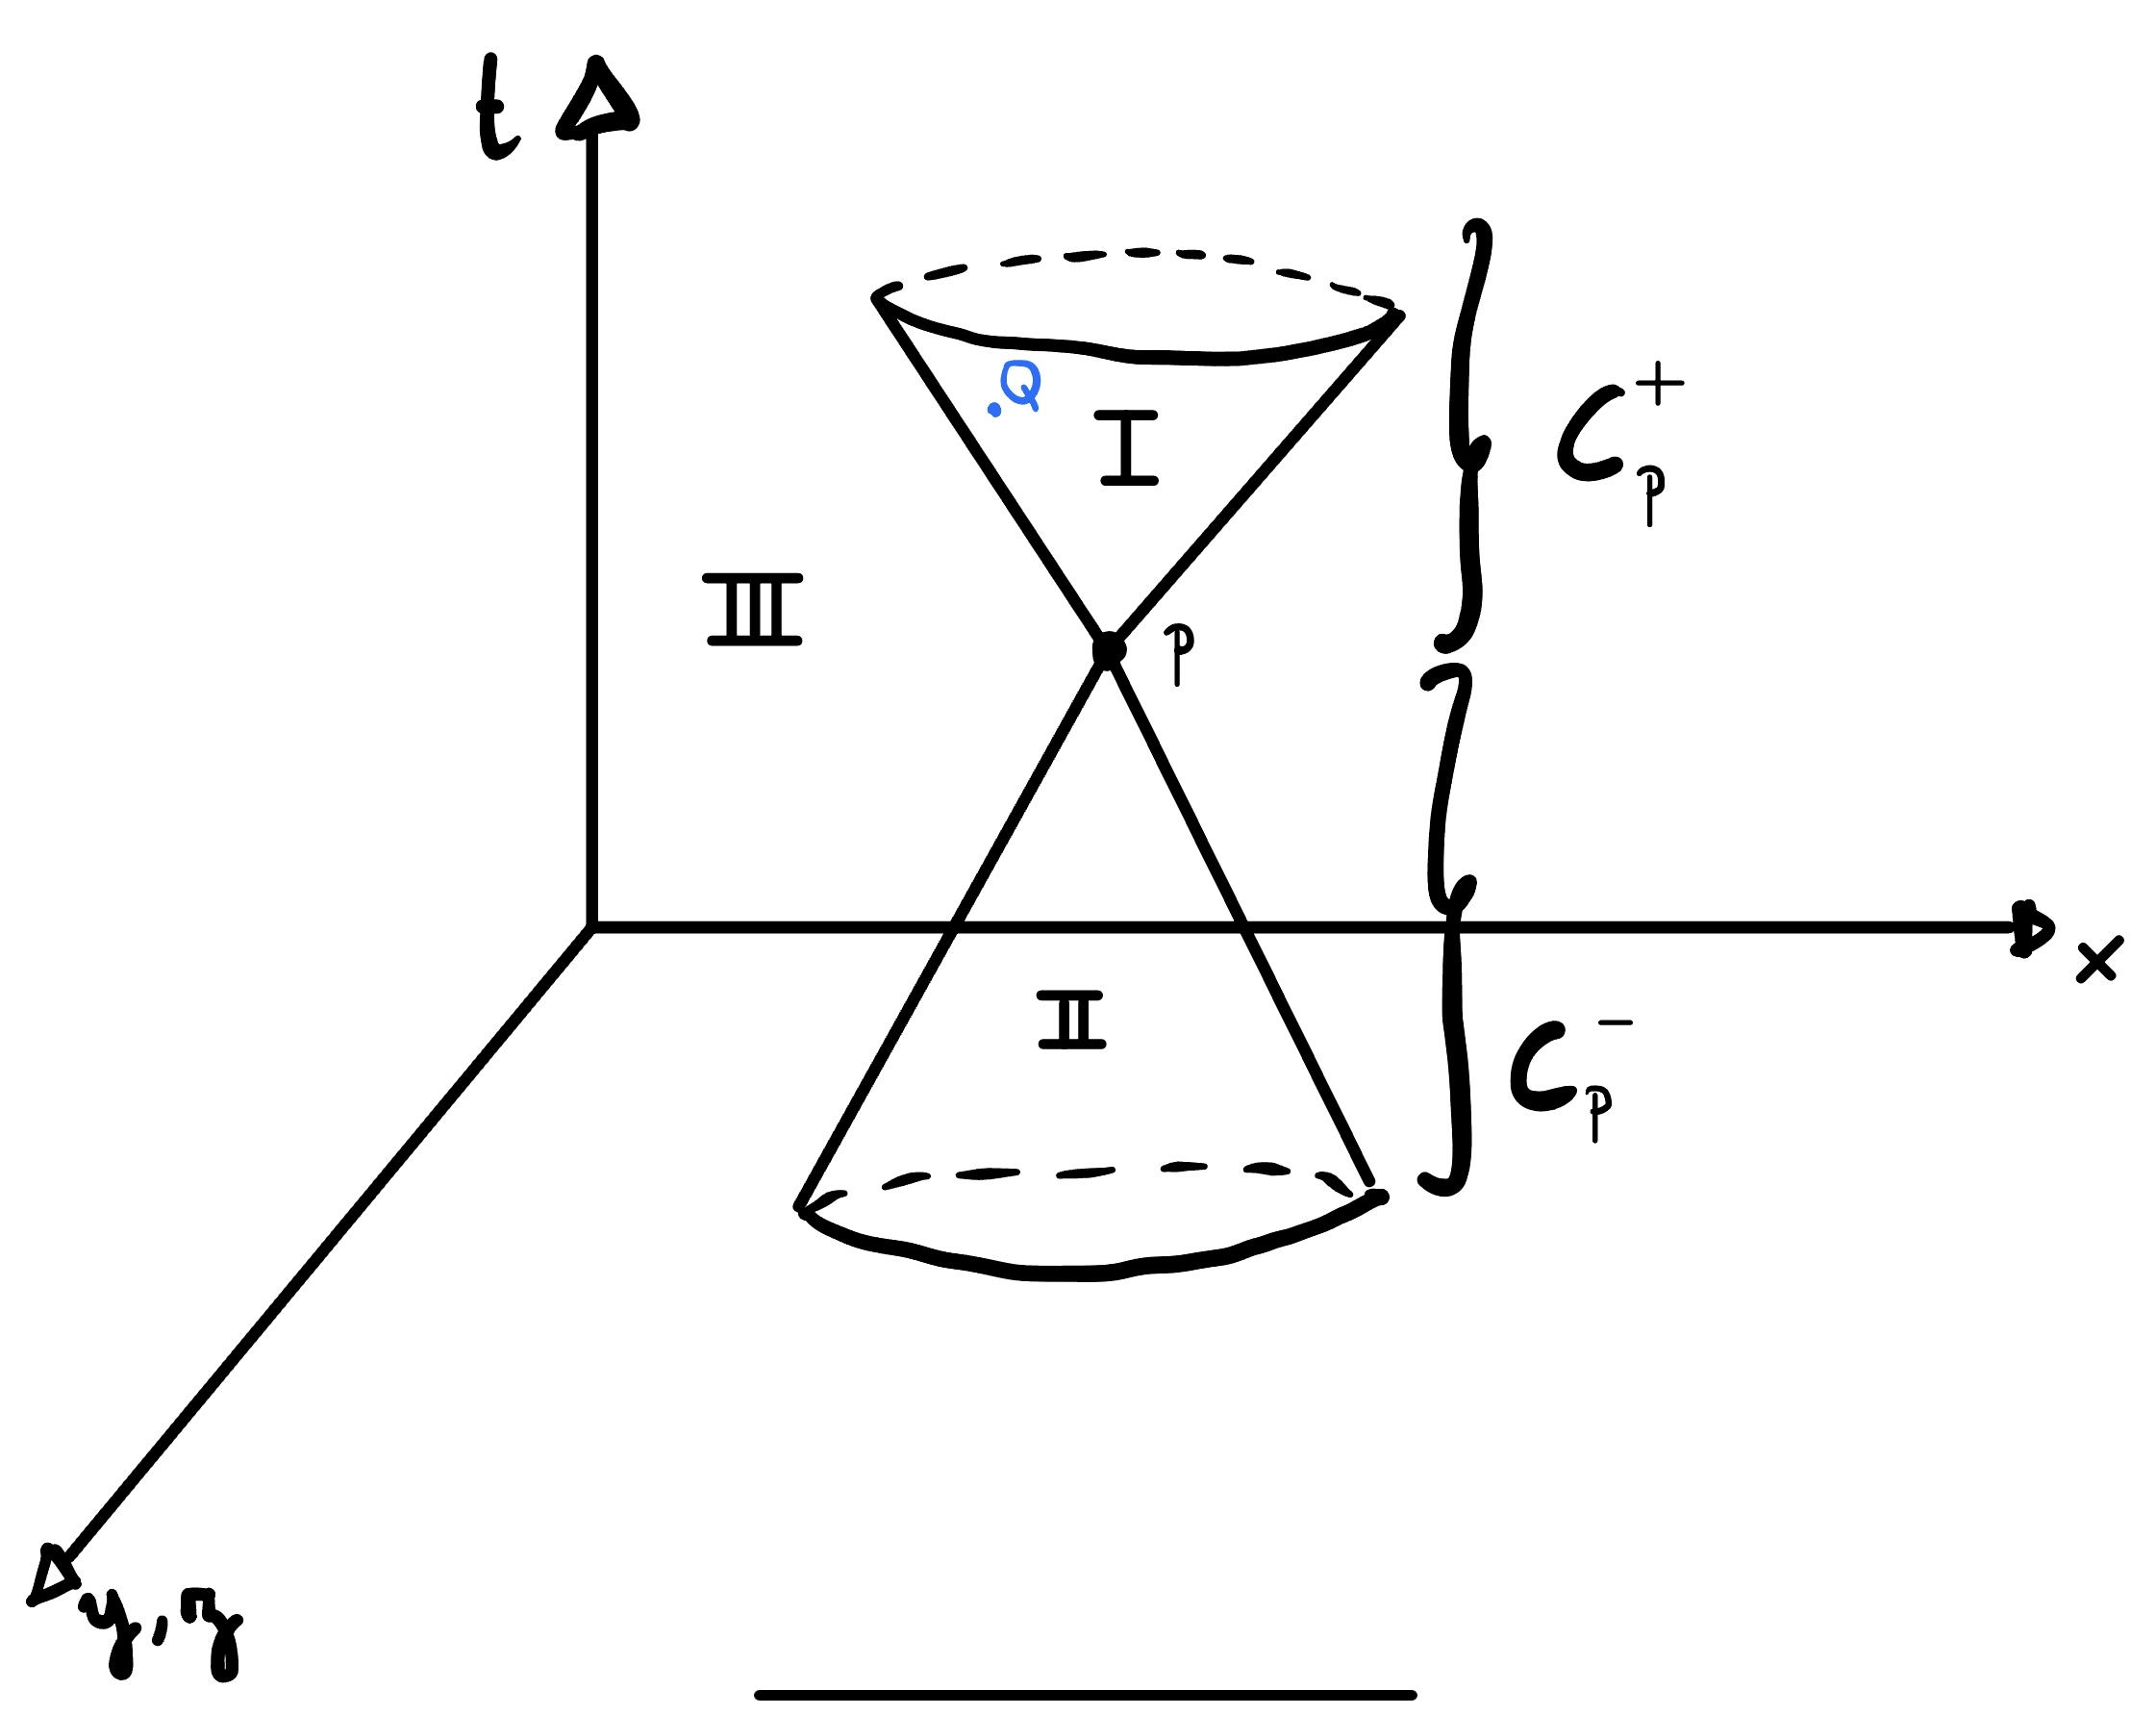
\includegraphics[width=0.5\textwidth]{Chapitres/2. Relativité Restreinte/Images/Cone de lumière avec point Q dans 1.jpg}
        \caption{Le cône de lumière de $P$ représenté dans l'espace $\R^{1,2}$}
        \label{fig:2.1}
\end{figure}

\begin{theoremframe}
    \begin{propri}
        Si $(\Delta s)^2_{PQ} < 0$ alors on peut trouver un référentiel inertiel pour lequel $P$ et $Q$ se passent au même endroit c'est-à-dire que $\Delta x^{i}_{PQ }= 0$.
    \end{propri}
\end{theoremframe}
\begin{proof}
    Exercice.
\end{proof}
    Comme on est dans le cas où $(\Delta s)^2_{PQ} < 0$ (intérieur du cône), $P$ et $Q$ sont en contact causal. Graphiquement, la propriété précédente est facile à démontrer, comme le montre la figure \ref{fig:2.2}. En effet, comme $Q$ se trouve à l'intérieur du cône de lumière de $P$, et en se rappelant de l'effet d'un boost sur les axes du nouveau référentiel $O'$, il est possible de trouver un référentiel dont l'axe de temps $t'$ relie $P$ à $Q$. Ainsi, $\Delta x = 0$. Il est en revanche impossible de trouver un référentiel inertiel dans lequel les deux évènements ont lieu en même temps.
\begin{figure}[H]
    \begin{center}
        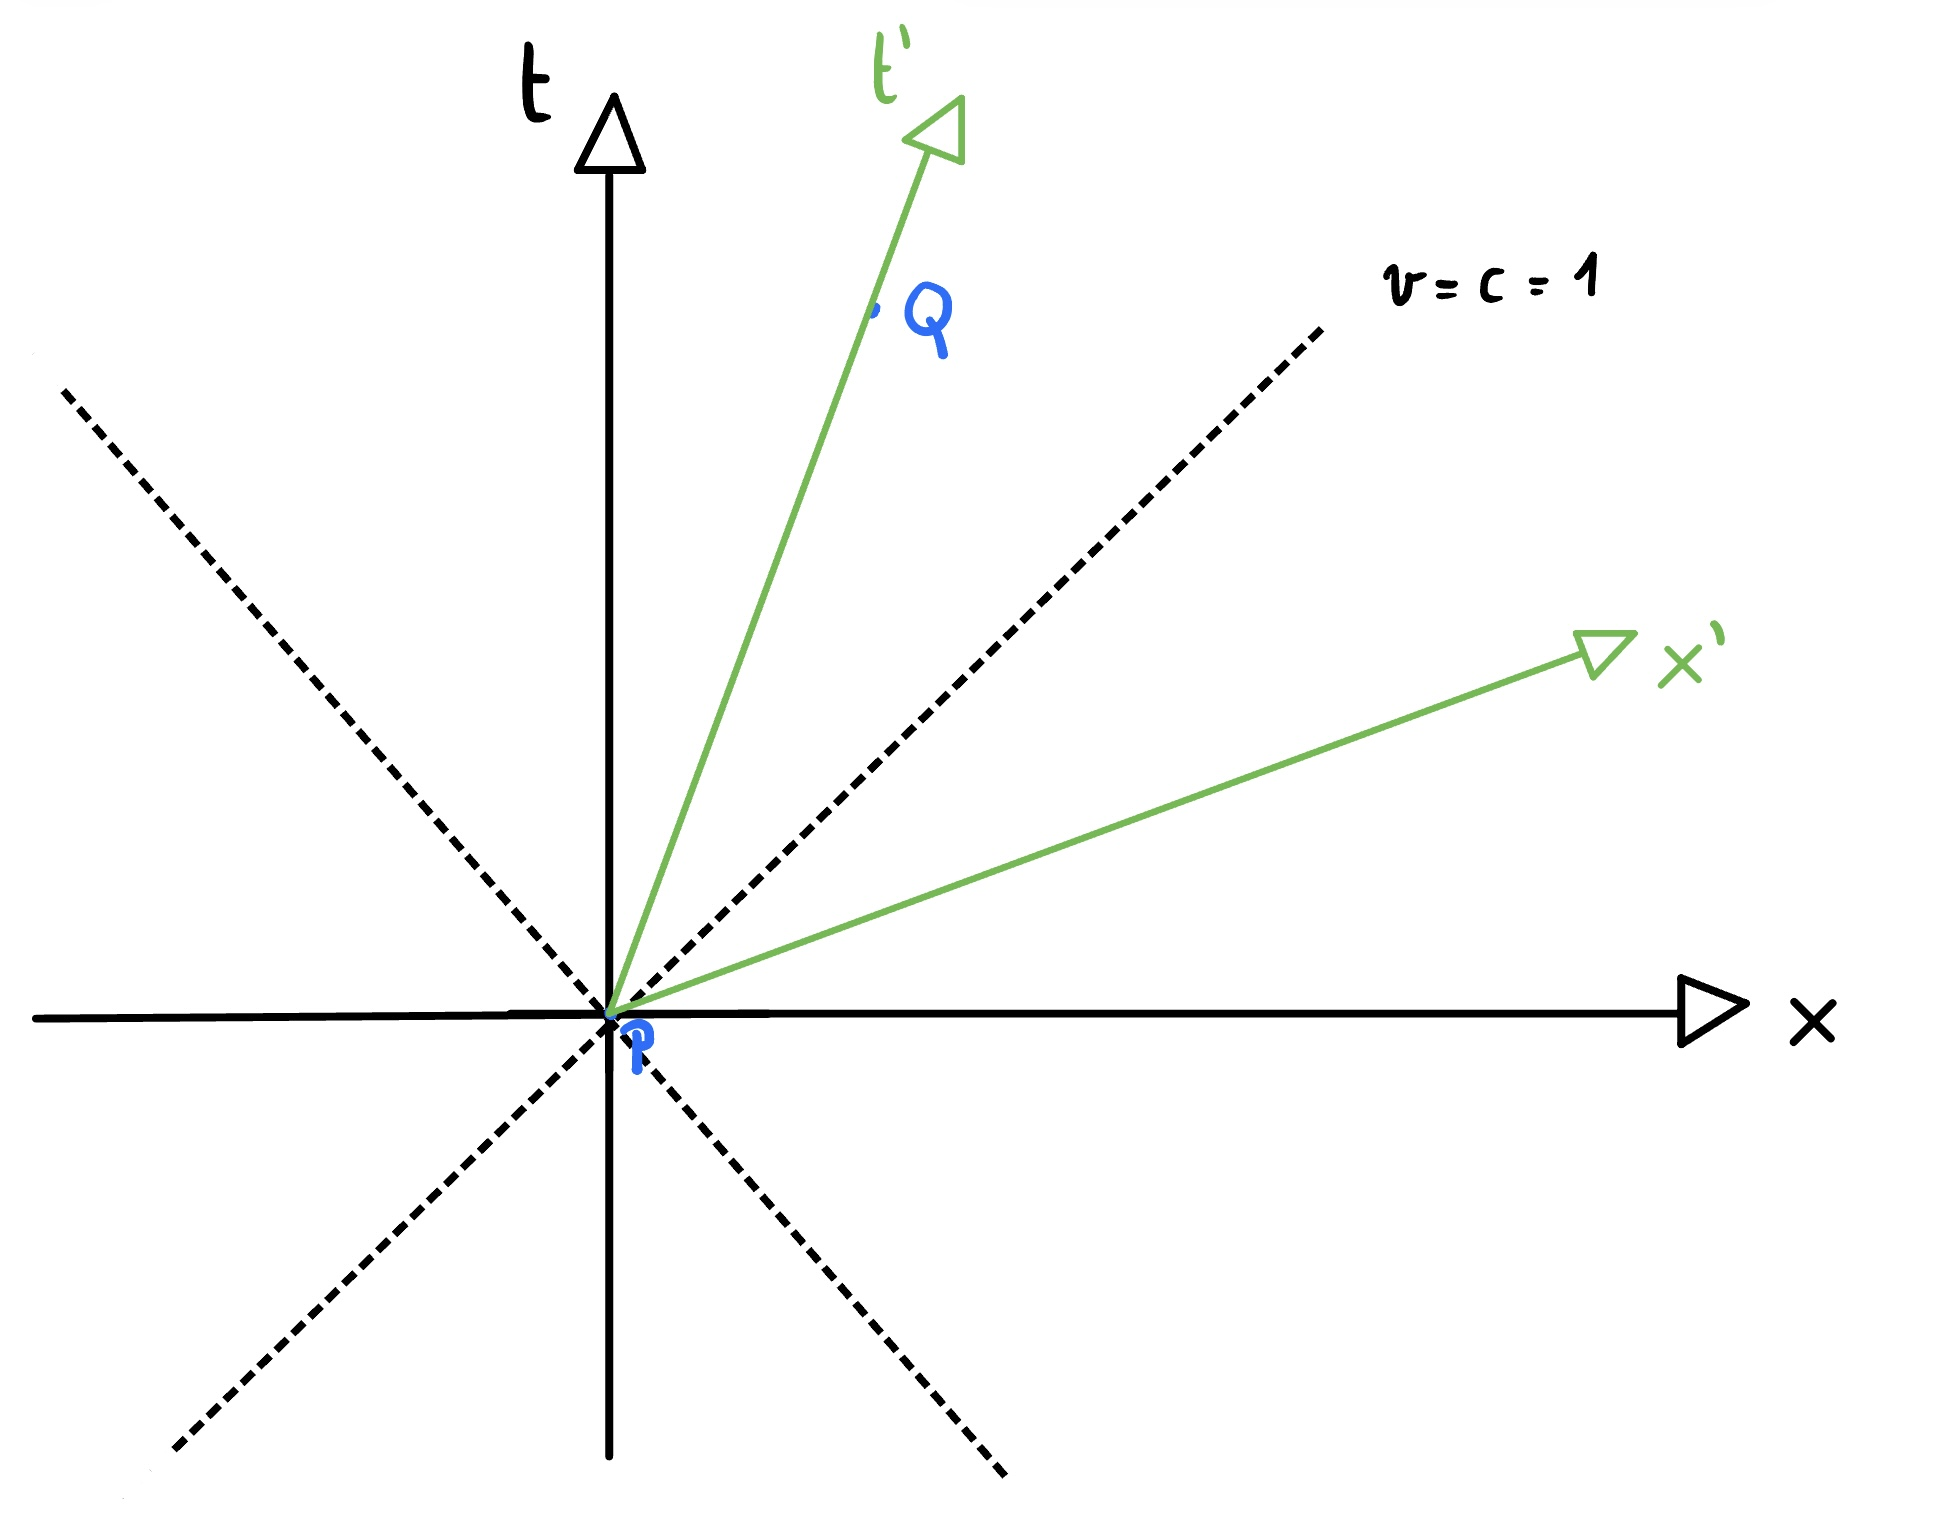
\includegraphics[scale=0.1]{Chapitres/2. Relativité Restreinte/Images/Changement de variable.jpg}
        \caption{Il existe un référentiel tel que deux points causalements connectés se passent au même endroit.}
        \label{fig:2.2}
    \end{center}
\end{figure}

\begin{theoremframe}
    \begin{propri}
        Si $Q$ appartient à l'ailleurs absolu de $P$, alors
        \begin{itemize}
            \item[\emph{(i).}] Il n'existe pas de référentiel inertiel tel que $Q$ se passe au même endroit que $P$.
            \item[\emph{(ii).}] Il est possible de trouver des référentiels inertiels tels que $Q$ se passe avant, en même temps ou après $P$.
        \end{itemize}
    \end{propri}
\end{theoremframe}
\begin{proof}
    Exercice.
\end{proof}

    Comme $Q$ n'est pas dans le cône de lumière, $P$ et $Q$ ne peuvent pas être en contact causal. On peut effectuer un boost tel que deux événements $P$ et $Q$ ont lieu en même temps ( c'est-à-dire que $\Delta t' = 0$). 

    Les cônes de lumière donnent à l'espace-temps de Minkowski une structure très différentes de l'espace-temps euclidien usuel de la théorie de Newton. Dans cette dernière, il n'y a pas de transformation mélangeant espace et temps , et il existe une division logique de l'espace-temps en "tranches ", représentant tout l'espace à un temps donné. En particulier:
    \begin{enumerate}
        \item la notation de simultanéité est absolue (non-ambiguë).
        \item les trajectoires d'une particule sont contraintes uniquement par $\Delta t> 0$. On peut avoir $v>c$
    \end{enumerate}
    En relativité restreinte, la notion de simultanéité devient relative au référentiel choisi et d'autre part, l'espace-temps est structuré par les cônes de lumières en tout point qui déterminent les trajectoires possibles des particules. Par l'invariance de $c$ pour tout référentiel inertiel, on peut déduire que les cônes de lumières sont les mêmes pour tout référentiel inertiel.
    \begin{figure}[H]
        \centering
        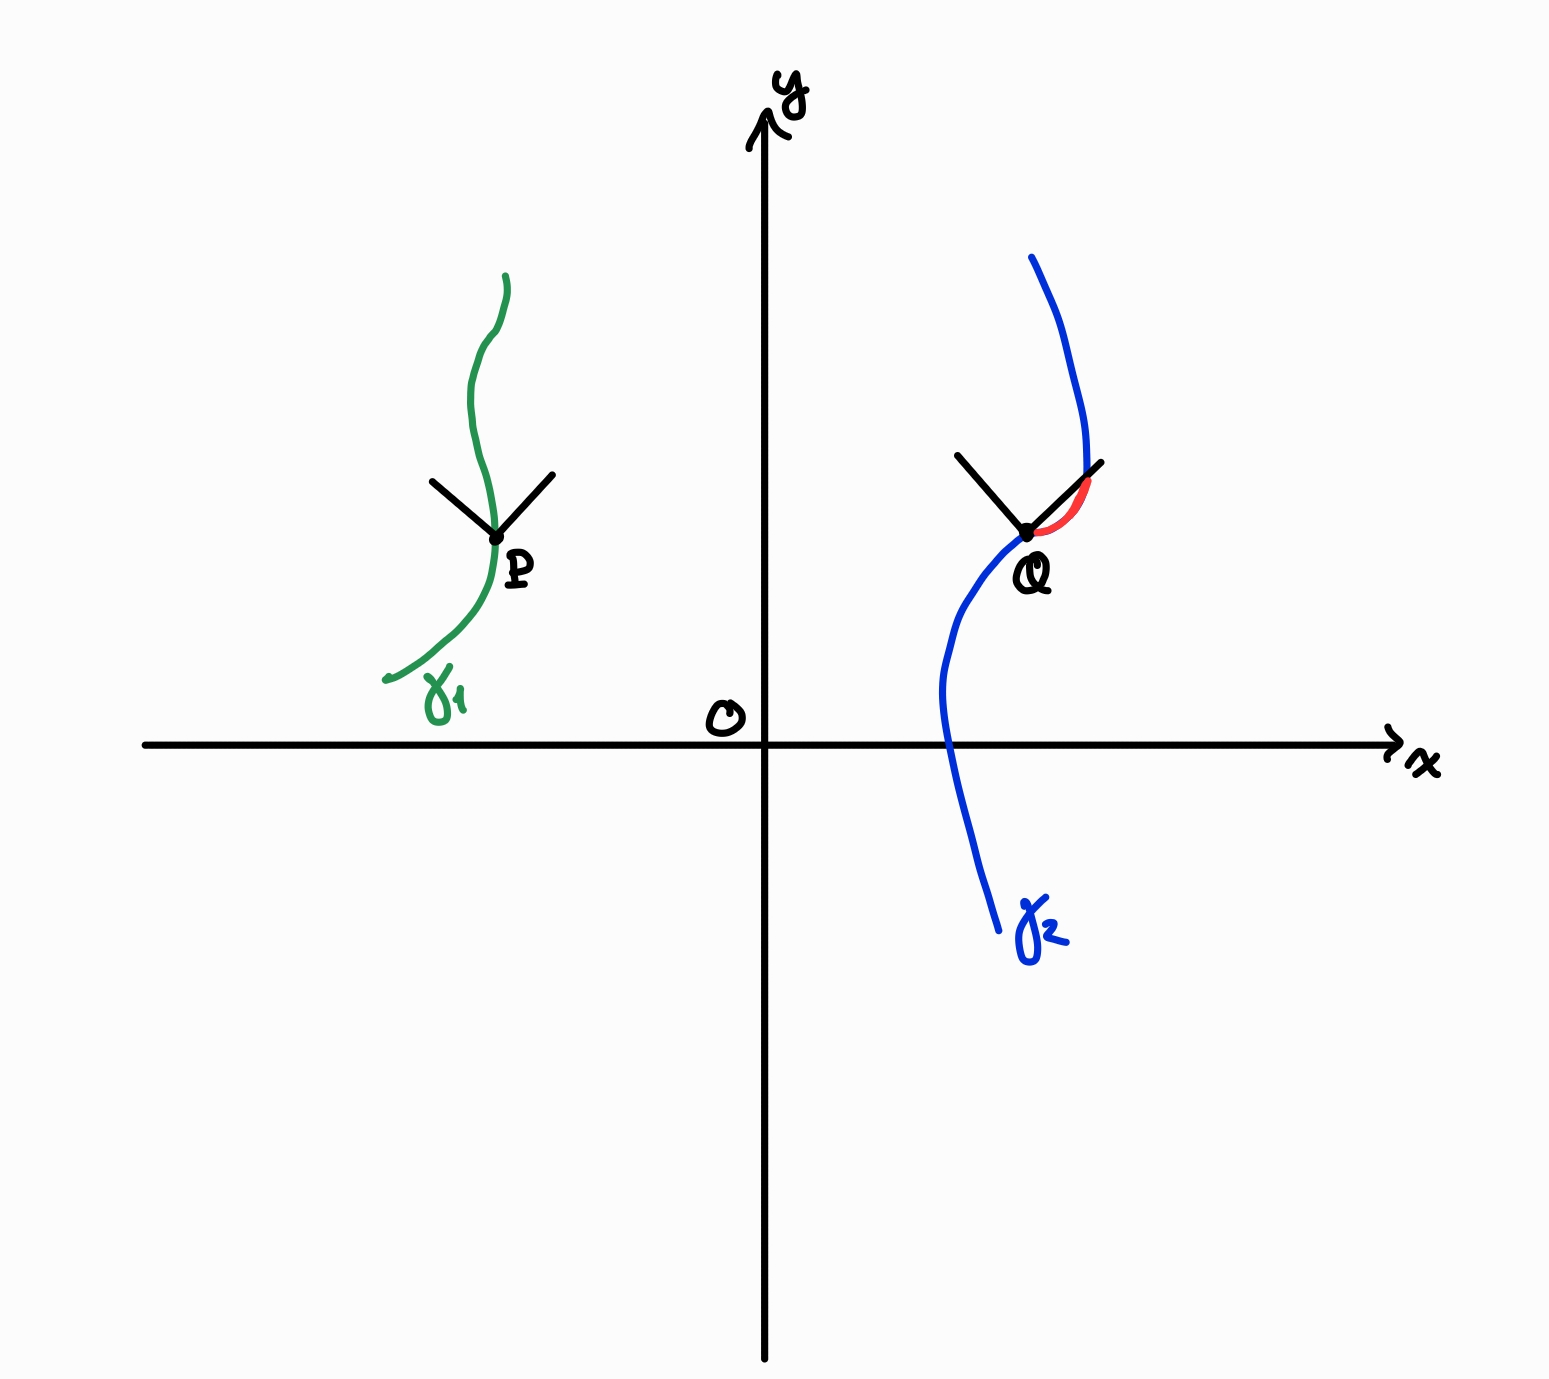
\includegraphics[width=0.5\linewidth]{Chapitres/2. Relativité Restreinte/Images/Courbes non causales.png}
        \caption{En $\R^{1,3}$, uniquement les trajectoires du type $\gamma_1$ sont admissibles. La courbe $\gamma_2$ ne peut pas représenter la trajectoire d'une particule car son tracé n'est plus contenu dans le cône de lumière de $Q$.}
        \label{fig:2.3}
    \end{figure}
\subsection{Temps propre}

Soient deux évènements $P$ et $Q$ causalement liés. 
\begin{theoremframe}
    \begin{defi}
        Le temps propre séparant $P$ et $Q$ est défini comme:
        \begin{equation}
            (\Delta s)^2_{PQ} = -(\Delta \tau)^2
        \end{equation}
    \end{defi}
\end{theoremframe}

Si $P$ et $Q$ représentent une particule libre à des temps différents, le temps propre $\Delta \tau $ est le temps écoulé entre deux évènements pour un observateur attaché au mouvement. En effet, comme les évènements sont causalement liés, il existe un référentiel dans lequel $P$ et $Q$ se passent au même endroit, et donc $(\Delta s)^2=-(\Delta t')^2 =$ et donc $\Delta t' = \Delta \tau$ dans ce référentiel.

\subsection{Courbes causales}
Rappelons la notion de courbe.
\begin{theoremframe}
    \begin{rap}
        Soit $I$, un ouvert de $\R$. Une application (lisse) $\R \to \mathcal{M}: \lambda \mapsto x^\mu (\lambda)$ est appelé courbe (lisse) sur $\mathcal{M}$. Le champ de vecteur tangent à la courbe $v$ est défini par
        \begin{equation}
            v^\alpha = \frac{\td x^\alpha}{\td \lambda}
        \end{equation}
    \end{rap}
\end{theoremframe}
La courbe est dite de genre $\left\{
\begin{array}{l}
 \text{temps} \\
 \text{espace}\\
 \text{lumière}
\end{array}
\right.$
si la norme du champ $ v^2 = v_{\alpha}v^{\alpha}$ 
$\left\{
\begin{array}{l}
 < 0 \\
 > 0\\
 = 0
\end{array}
\right.$
\\
\begin{exmp}
    La norme du vecteur $v = (1,0,0,0)$ est donnée par $\eta_{\alpha \beta}v^{\alpha} v^{\beta} = (-1)v^{0} v^{0} =-1$. La norme n'est donc pas définie positive (comme dans le cas euclidien).
\end{exmp}
\begin{theoremframe}
    \begin{defi}
        Une courbe est dite causale si à tout point de la courbe, le vecteur tangent est
        \begin{itemize}
            \item[(i).] de genre temps ou lumière.
            \item[(ii).] orienté vers le futur ($\frac{\td x^0}{\td\lambda}>0$).
        \end{itemize}
    \end{defi}
\end{theoremframe}
\subsection{Longueur Minkowski d'une courbe causale}

D'après la définition du temps propre de deux évènements causalement liés
\begin{equation}
    \label{eq:temps propre}
   (\Delta \tau)^{2} = -(\Delta s)^2 = (\Delta t)^2 - \sum_{i}(\Delta x^{i})^2 
\end{equation}

on définit le temps propre infinitésimal
\begin{equation}
    d\tau ^2 = -ds^{2} = dt^2 - \sum_{i} (dx^{i})^2
\end{equation}
\begin{figure}
    \centering
    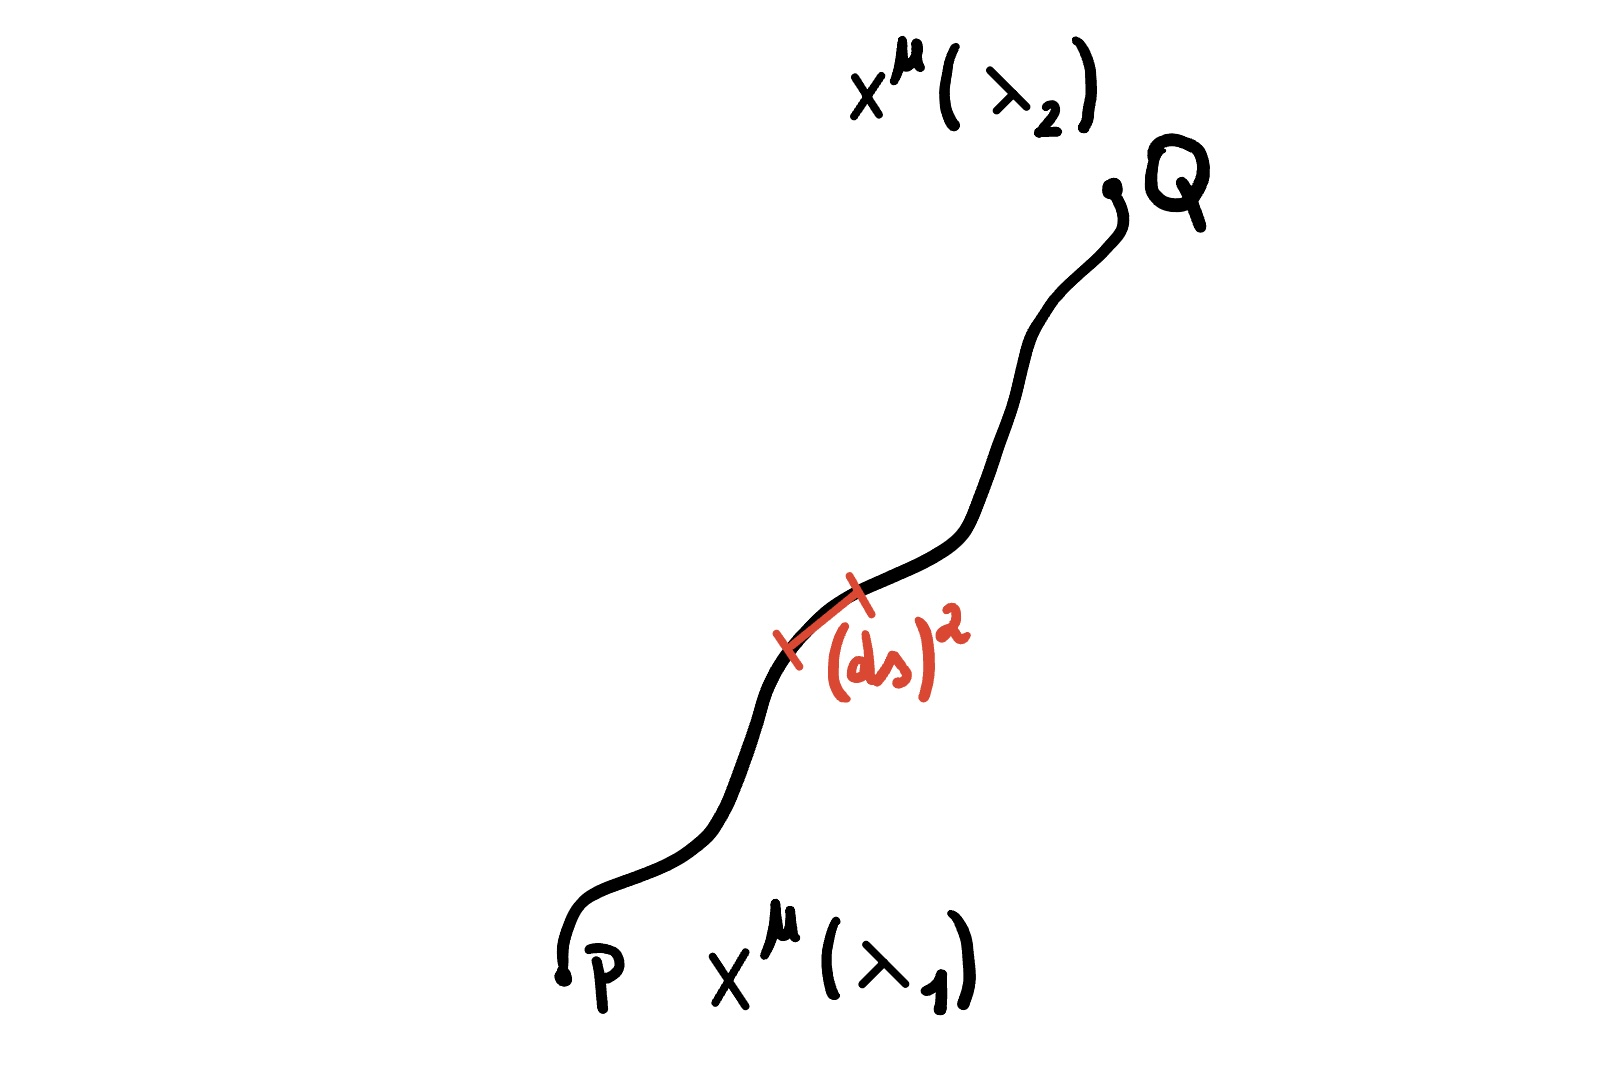
\includegraphics[width=0.5\linewidth]{Chapitres/2. Relativité Restreinte/Images/Coubre.jpg}
    \caption{}
    \label{fig:2.4}
\end{figure}

Cette définition permet nous permet de définir le temps propre d'une courbe causale $\gamma$ arbitraire comme

\begin{align}
    \tau_\gamma &= \int_{\gamma} \td\tau\\
    &= \int^{\lambda_{2}}_{\lambda_{1}}\left(\frac{\td\tau}{\td\lambda}\right)\td\lambda\\
    &= \int^{\lambda_{2}}_{\lambda_{1}} \td \lambda\sqrt{\left(\frac{\td t}{\td\lambda}\right)^2 - \sum_{i}\left(\frac{\td x^{i}}{\td\lambda}\right)^2} 
\end{align}

Et est le temps mesuré par un observateur qui suit la trajectoire. 
\begin{theoremframe}
    \begin{propri}
        Le temps propre entre deux évènements causalement reliés défini par \ref{eq:temps propre} correspond au temps propre de la droite reliant les deux évènements. De plus, la courbe qui maximise le temps propre entre deux évènements est la droite.
    \end{propri}
\end{theoremframe}
\begin{proof}
    Exercice.
\end{proof}
En effet, le temps propre de deux courbes causales distinctes reliant deux évènements n'est en général pas identique. Un exemple de cette propriété est le paradoxe des jumeaux.

\begin{exmp}[Paradoxe des jumeaux\footnote{Disclaimer: il s'agit d'une expérience de pensée. Aucune fusée n'a été blessée au cours de cette expérience.}]
    Supposons que deux jumeaux sur Terre possèdent chacun·es une horloge atomique qui affiche la même heure. Posons leur genre = M. L'un des jumeaux est envoyé dans l'espace à une vitesse proche de celle de la lumière avec cette horloge. Quand il revient sur Terre, en comparant les deux horloges, le jumeaux étant resté sur terre est plus jeune que celui parti dans l'espace. 
\end{exmp}
Pour expliquer ce "paradoxe" (ce n'en est pas réellement un\footnote{En fait, si, selon la définition. \href{https://www.youtube.com/watch?v=ppX7Qjbe6BM}{Vidéo intéressante sur le sujet}.}), intéressons-nous à la situation simplifiée suivante, où un jumeau passe directement de $A$ à $C$, et l'autre jumeau fait un détour par $B'$.
\begin{figure}[H]
    \centering
    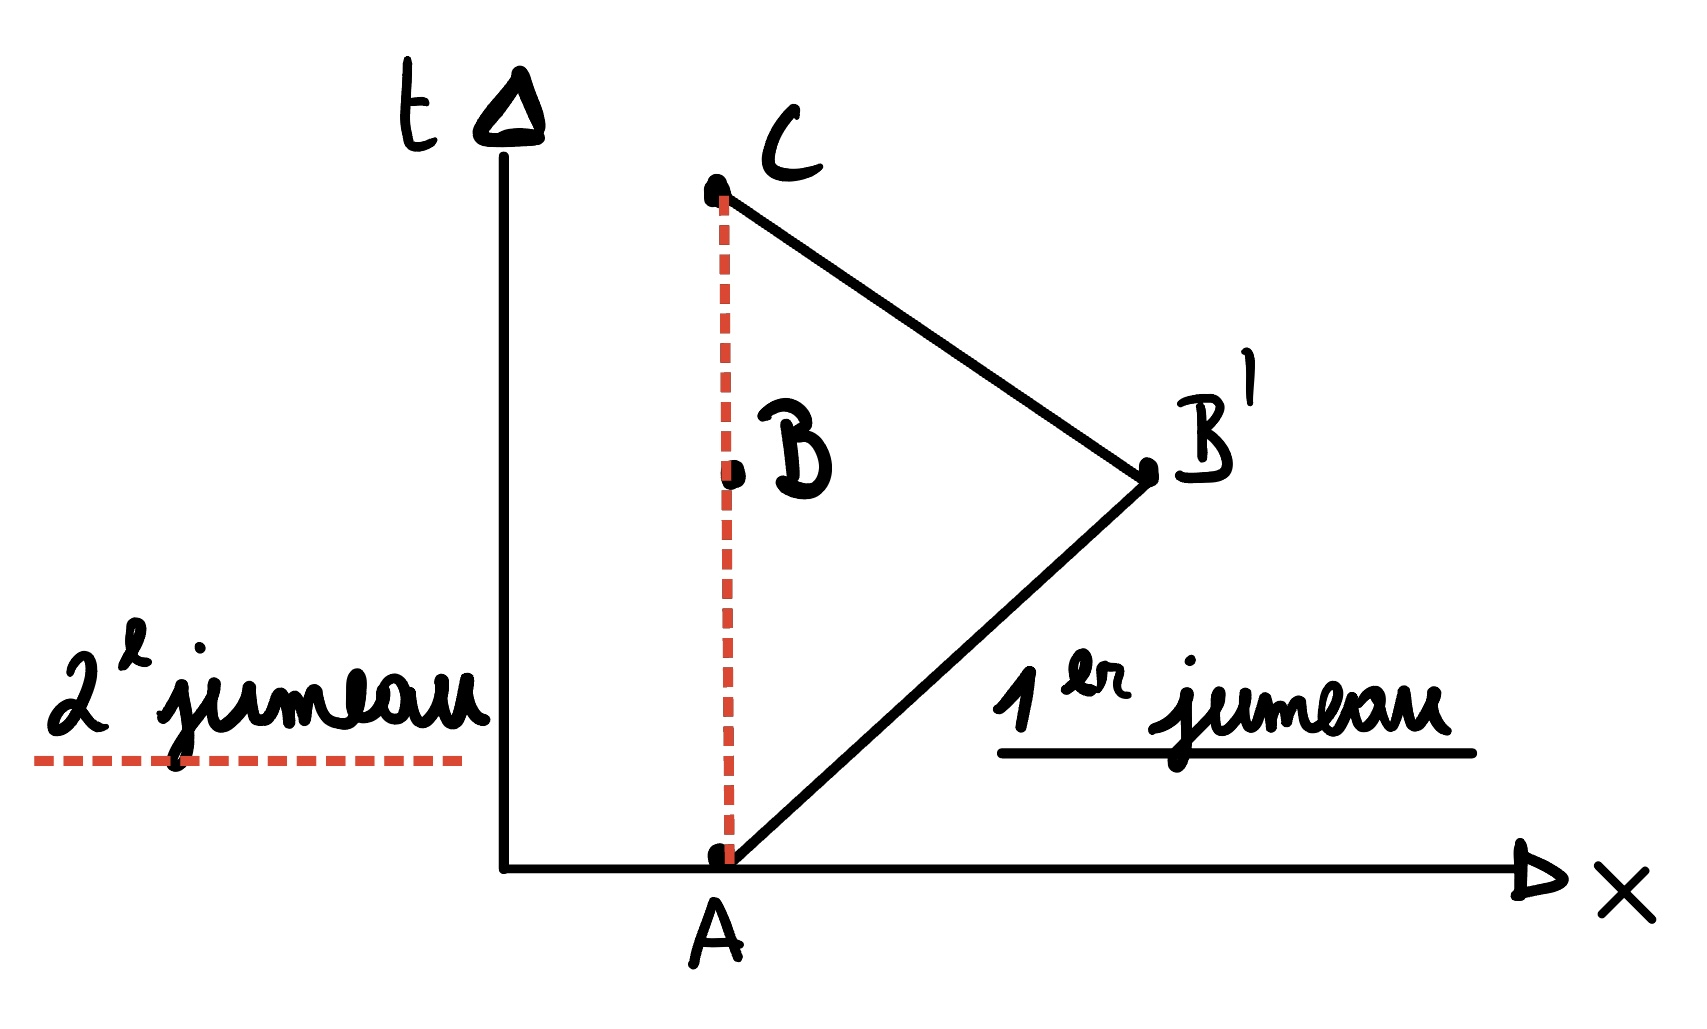
\includegraphics[width=0.5\linewidth]{Chapitres/2. Relativité Restreinte/Images/Deux jumeaux.jpg}
    \caption{}
    \label{fig:2.5}
\end{figure}

Calculons le temps propre des deux chemins. Dans le référentiel $O$, on a pour le deuxième jumeau
\begin{equation}
    (\Delta \tau_{ABC})^2 = (\Delta t)^2
\end{equation} 
Alors que comme $B'=(\frac{\Delta t}{2},\Delta x)$,

\begin{align}
        (\Delta \tau_{AB'C})^2 &= (\Delta \tau_{AB'} + \Delta \tau_{B'C})^2\\
        &= 4(\Delta \tau_{AB'})\\
        &= 4 \left(\left(\frac{\Delta t}{2}\right)^2 - (\Delta x)^2\right)\\
        &= 4 \left(\left(\frac{\Delta t^2}{4}\right) - (\Delta x)^2\right)
    \end{align}
    On peut définir $v = \dfrac{\Delta x}{(\Delta t/2)} = \dfrac{2 \Delta x}{\Delta t}$ qui est tel que $v^2 = \frac{4(\Delta x)^2}{(\Delta t)^2}$ et donc
    \begin{align*}
        (\Delta \tau_{AB'C})^2 &= (\Delta t)^2(1 - v^2)\\
        &< (\Delta t)^2
    \end{align*}

Le temps propre du premier jumeaux (voyageur) est plus petit que le temps propres du jumeau 2 (au repos). 
\begin{center}
    \textit{Le temps s'écoule plus lentement quand on est en mouvement.}
\end{center}

\subsection{Horizon des événements} 

Soit $\mathcal{S} \in \R^{1,3}$  un sous-ensemble de Minkowski. 
\begin{theoremframe}
    \begin{defi}
        Le futur chronologique $I^{+}(\mathcal{S})$ est l'ensemble des points de $\R^{1,3}$ qui sont reliés à un point de $\mathcal{S}$ par une courbe causale de genre temps. 
    \end{defi}
\end{theoremframe}
\begin{theoremframe}
    \begin{defi}
        Le futur causal $J^{+}(\mathcal{S})$ est l'union de $\mathcal{S}$ avec tous les points de $\R^{1,3}$ qui sont reliés à un point de $\mathcal{S}$ par une courbe causale. 
    \end{defi}
\end{theoremframe}

\begin{exmp}
    Si $\mathcal{S} = \{P\}$ alors $I^{+}(\mathcal{S}) = \mathrm{int}( C_{P}^{+})$ et $J^{+}(\mathcal{S}) = C_{P}^{+} \cup \{P\}$. 
\begin{figure}[H]
    \centering
    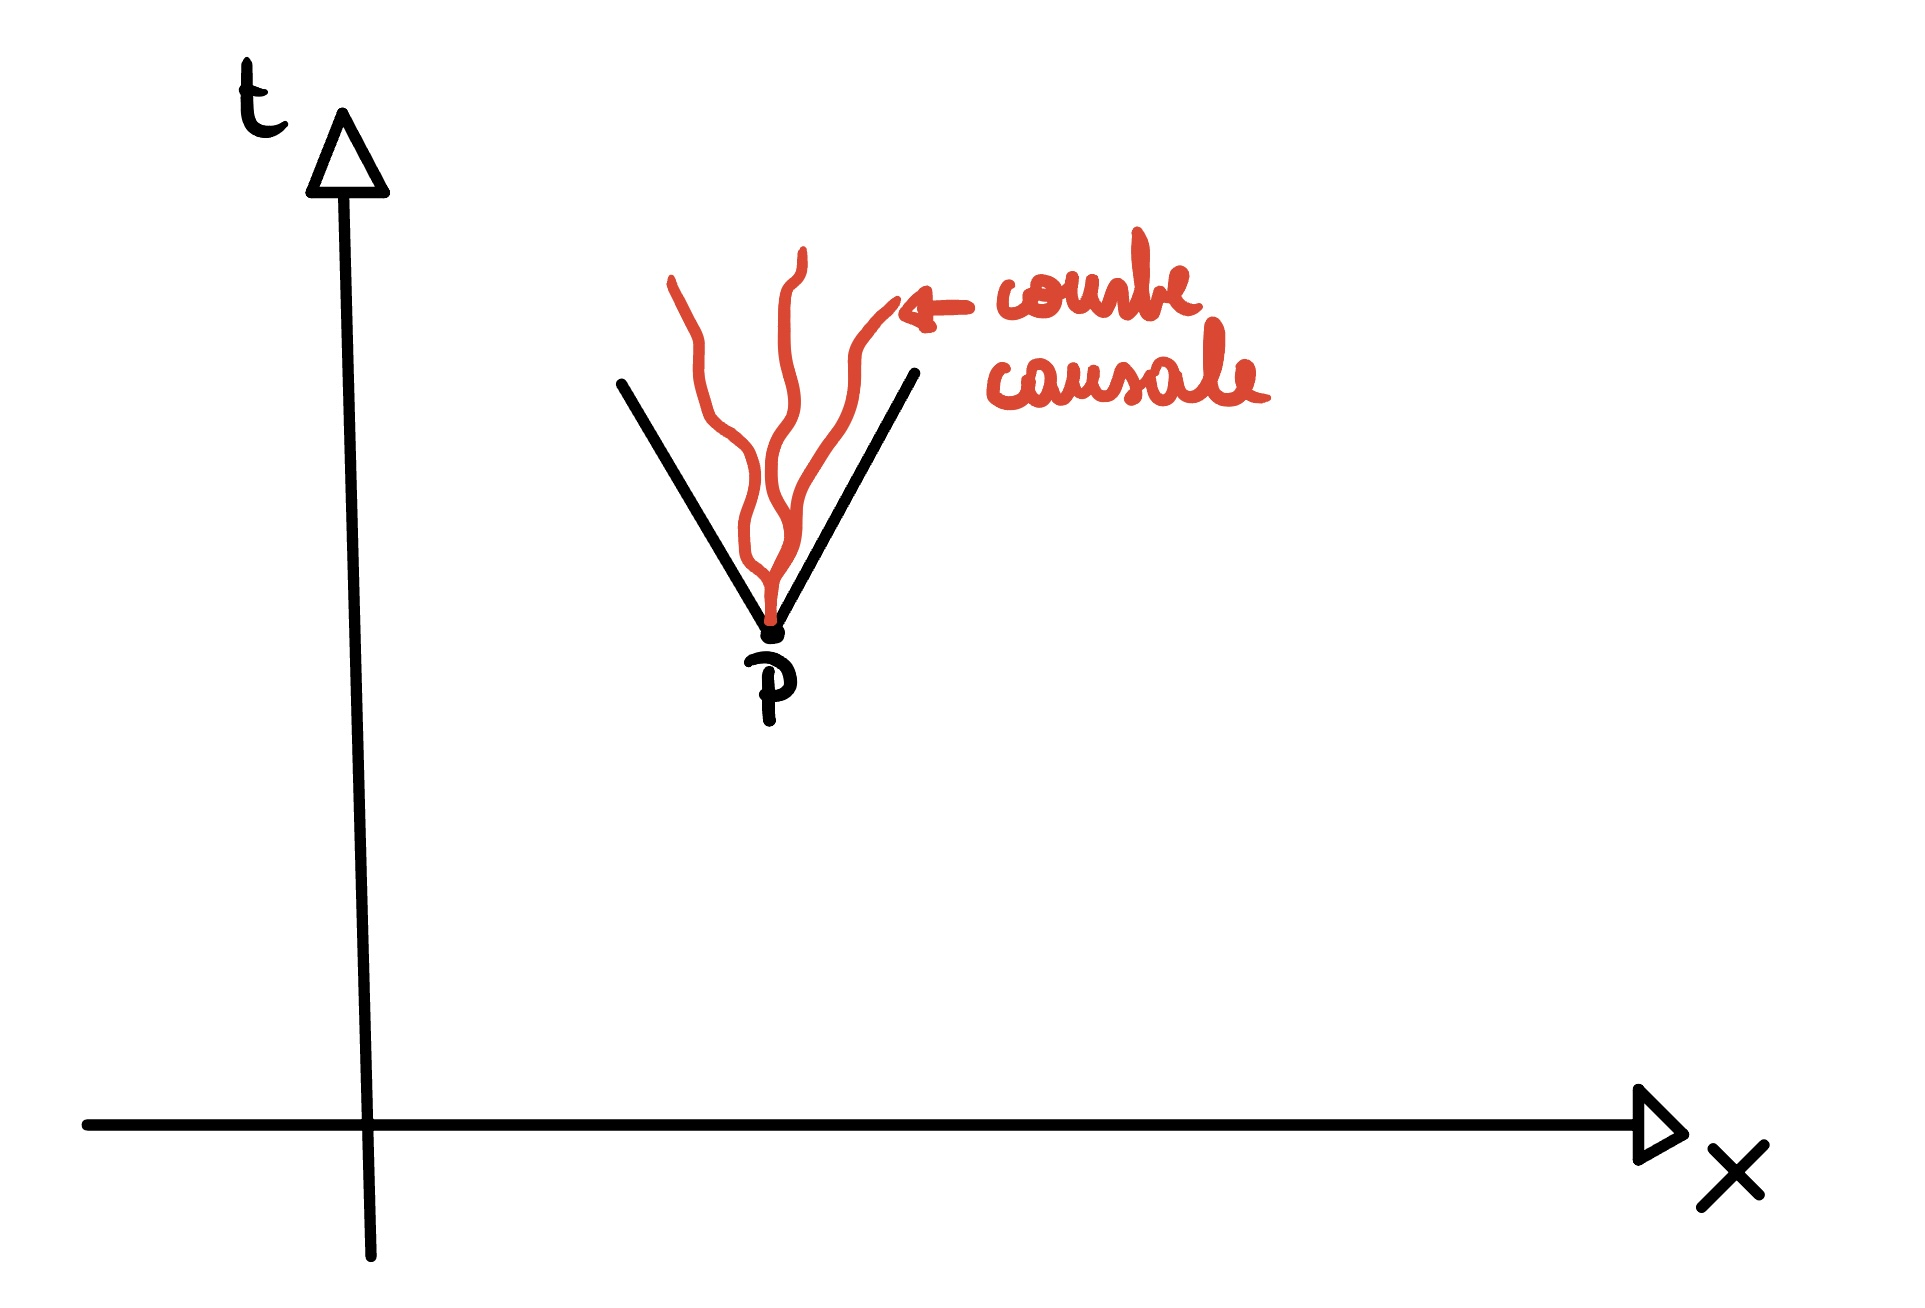
\includegraphics[width=0.5\linewidth]{Chapitres/2. Relativité Restreinte/Images/exemple1.jpg}
    \caption{}
    \label{fig:2.6}
\end{figure}
\end{exmp}

    \begin{exmp}
    Si $\mathcal{S}$ est la trajectoire d'un observateur inertiel au repos, alors $I^{+}(\mathcal{S}) = J^{+}(\mathcal{S}) = \R^{1,3}$ tout entier.
    \begin{figure}[H]
        \centering
        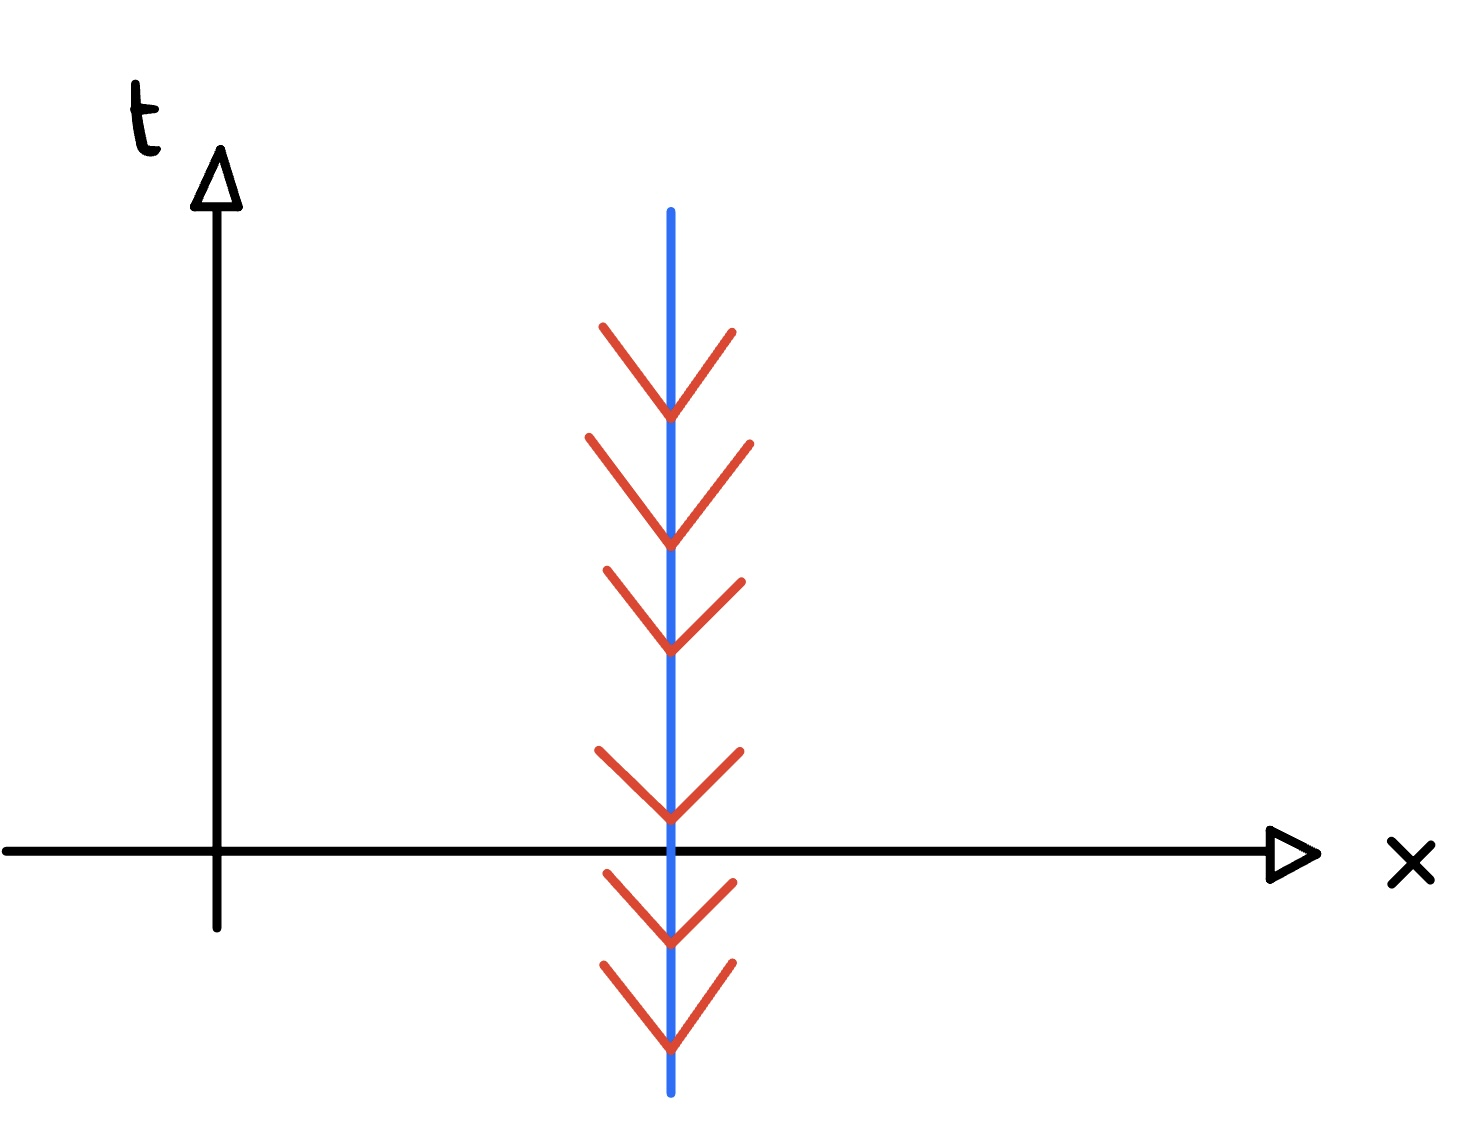
\includegraphics[width=0.5\linewidth]{Chapitres/2. Relativité Restreinte/Images/exemple2.jpg}
        \caption{}
        \label{fig:2.7}
    \end{figure}
\end{exmp}
\begin{exmp}[Expérience de Rindler\footnote{Attention aux débutant·es, il s'agit de nouveau d'une expérience de pensée !}]
    Considérons maintenant le cas d'un observateur accéléré. Soit $x^{\alpha}(\lambda)$, une courbe de genre temps. Alors
    
    \begin{equation}
    \eta_{\alpha \beta} \frac{\td x^{\alpha}}{\td \lambda}\frac{\td x^{\beta}}{\td \lambda} = -\alpha^2(\lambda) < 0
    \end{equation}

    On souhaite effectuer un changement de variable $\lambda \to \mu$ tel que $\alpha(\mu) = 1$.

    \begin{equation*}
        \eta_{\alpha \beta} \frac{\td x^{\alpha}}{\td \mu}\frac{\td x^{\beta}}{\td \mu} \left(\frac{\td \mu}{\td \lambda}\right)^2 = -\alpha(\lambda)^2
    \end{equation*}

    Ainsi, on peut choisir $ \mu (\lambda )$ tel que $\left(\dfrac{\td \mu}{\td \lambda}\right)^2 = \alpha(\lambda)^2$.

    Ce qui implique que: 

    \begin{equation*}
         \eta_{\alpha \beta} \frac{\td x^{\alpha}}{\td \mu}\frac{\td x^{\beta}}{\td \mu} = -1
    \end{equation*}
    On peut écrire $\mu (\lambda )$ de manière infinitésimal tel que $-d\mu ^2 = \eta_{\alpha \beta} \td x^{\alpha} \td x^{\beta} = \td s^2 = -d\tau^2$ et donc $x^{\alpha}(\mu) = x^{\alpha}(\tau)$, soit

    \begin{equation*}
        \eta_{\alpha \beta} \frac{\td x^{\alpha}}{\td \tau}\frac{\td x^{\beta}}{d \tau} = -1
    \end{equation*}

    La 4-vitesse le long d'une courbe est définie par:

    \begin{equation*}
        v^{\alpha} = \frac{\td x^{\alpha}}{\td \mu}
    \end{equation*}

    où $v^{\alpha} v_{\alpha} = -1$.

    La 4-accélération est définit par: 

     \begin{equation*}
        a^{\alpha} = \frac{\td v^{\alpha}}{\td \mu}
    \end{equation*}
    Nous souhaitons étudier la trajectoire d'un observateur à accélération constante, qui est un observateur tel que: 
    \begin{equation*}
        a_{\alpha}a^{\alpha} = a^{2} = \text{cste}
    \end{equation*}
    Choisissons un référentiel tel que l'accélération se fait dans la direction $x^{1}$ et décrit un mouvement dans le plan $(x^{0}, x^{1})$. Nous supposerons que $v^2 = v^3 = 0$. Les équations du mouvement pour cet observateur accéléré sont
\begin{align}
  \dfrac{d x^{\alpha}}{d \tau} = v ^{\alpha}\\
 \dfrac{d v^{\alpha}}{d \tau} = a^{\alpha}
\end{align}
muni des conditions
\begin{align}
    v^{\alpha}v_{\alpha} & = -1 = -(v^{0})^2 + (v^{1})^2\\
    a^{\alpha}a_{\alpha} & = a^2 = -(a^{0})^2 + (a^{1})^2 = \mathrm{cste}
\end{align}

Or, comme $v^{\alpha}v_{\alpha} = -1$:

\begin{align}
    \frac{\td v^\alpha v_\alpha}{\td \tau} &= 2 a^{\alpha}v^{\alpha} = 0 \\
    \implies &-a^{0}v^{0} + a^{1}v^{1} = 0\\
    \label{eq:2.57}
    \implies &v^{1} = \frac{v^{0}a^{0}}{v^{1}}
\end{align}

En adoptant temporairement des indices covariants purement pour question de visibilité:

\begin{align}
    a_1^2 &= 1 \cdot a_1^2\\
    &= \lt v_0^2 - v_{1}^2 \rt a_{1}^2\\
    &= v_{0}^2 \lt 1 - \frac{a_0^2}{a_1^2} \rt a_1^2\\
    &= v_{0}^2(a_{1}^2 - a_{0}^2)\\
    &= v_{0}^2 a^2
\end{align}

Nous obtenons donc que $a^1 = av^{0}$ et que $a^0 = av^{1}$ par \ref{eq:2.57}. Ce problème peut se réécrire en forme matricielle comme:
\begin{equation}
\frac{\td }{\td \tau} \begin{pmatrix}
    v^0 \\
    v^1
\end{pmatrix} = \begin{pmatrix}
    0 & a \\
    a & 0
\end{pmatrix}
\begin{pmatrix}
    v^0 \\
    v^1
\end{pmatrix}
\end{equation} 

La solution de ce système est

$\Rightarrow $\begin{equation*} \left\{
\begin{array}{l}
  v^{0} = \cosh{a\tau}\\
 v^{1} = \sinh{a\tau}\\
\end{array}
\right.
\end{equation*}

Et la position est donc donné par

$\Rightarrow $\begin{equation*} \left\{
\begin{array}{l}
  x^{0} = \frac{1}{a}\sinh{a\tau}\\
 x^{1} = \frac{1}{a}\cosh{a\tau}\\
\end{array}
\right.
\end{equation*}

À quoi ressemble cette trajectoire graphiquement ? On a que:

\begin{align*}
    &v^{1} = 0|_{\tau = 0}\\
    &(x^1)^2 - (x^0)^2 = \frac{1}{a^2}
\end{align*}

il s'agit donc d'une branche d'hyperbole.
\begin{figure}[H]
    \centering
    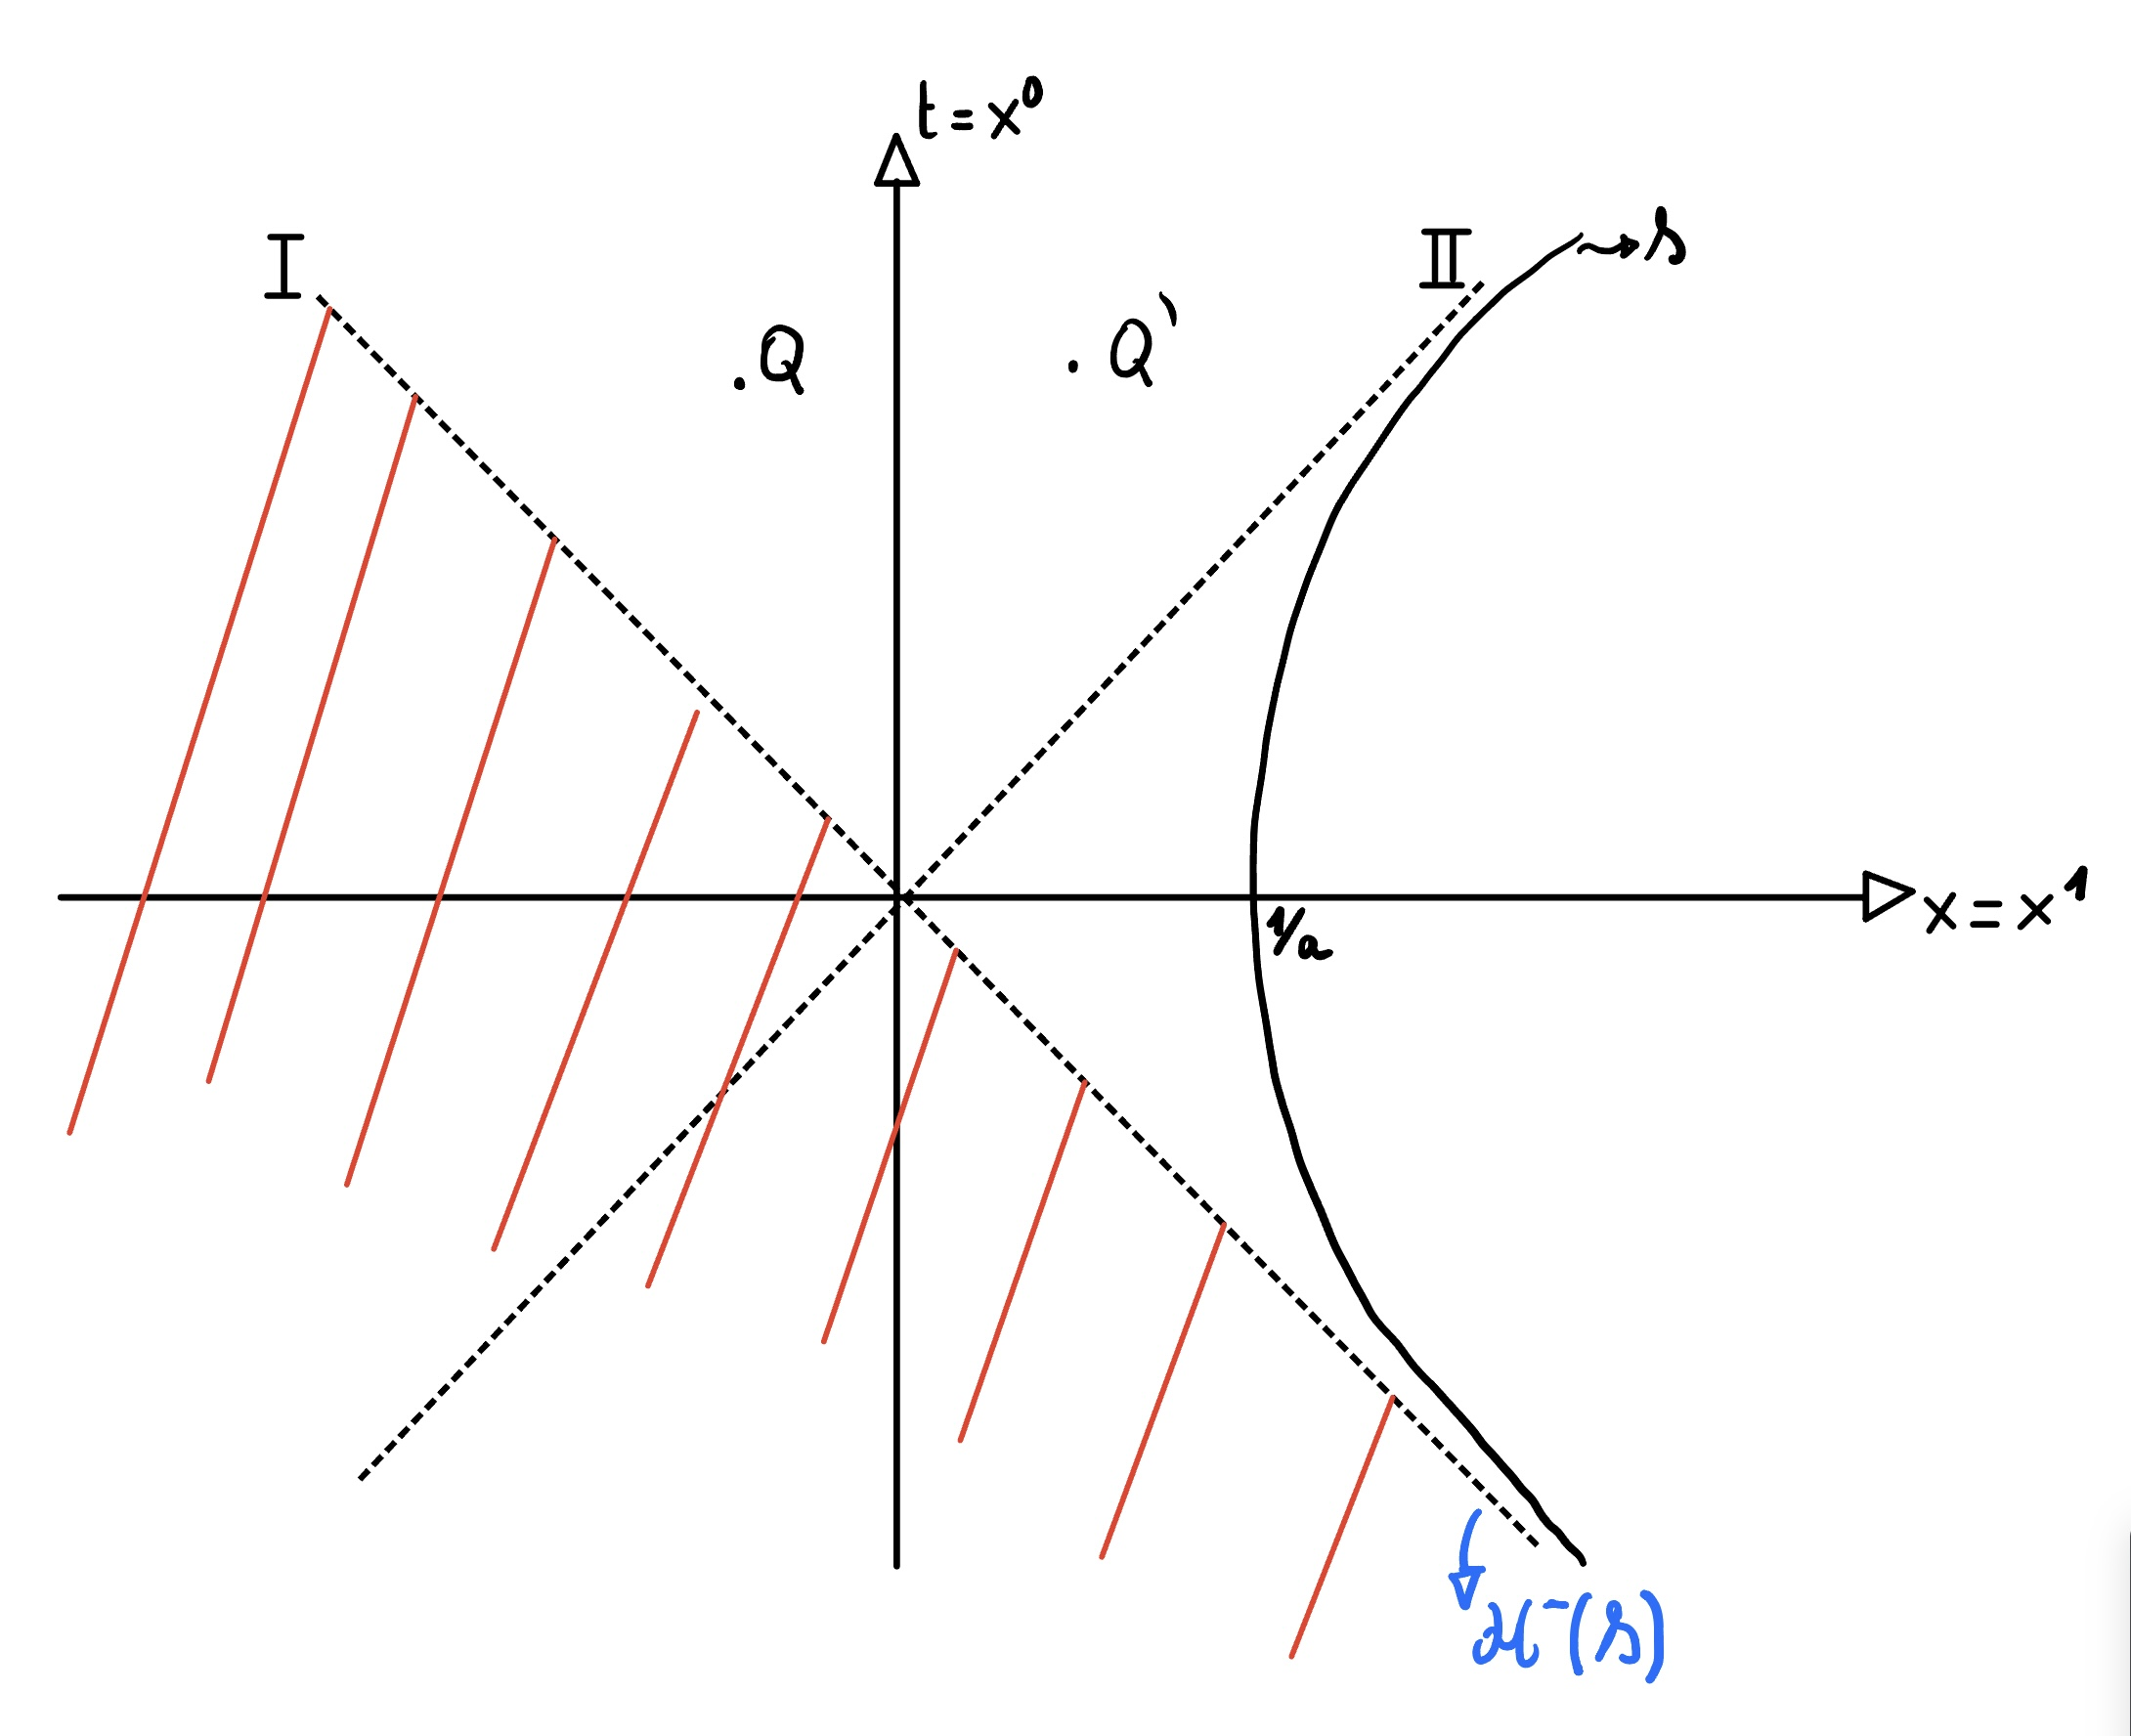
\includegraphics[width=0.5\linewidth]{Chapitres/2. Relativité Restreinte/Images/Courbe hyperbole 1.jpg}
    \caption{}
    \label{fig:2.8}
\end{figure}

Cette ensemble de points $\mathcal{S}$ est la trajectoire d'un observateur accéléré dans l'espace-temps de Minkowski. Quelques remarques:
\begin{enumerate}
    \item $\mathcal{S}$ ne pourra jamais influencer ce qui se trouve sous la ligne de lumière \cRM{1} (indiqué en rouge sur la figure \ref{fig:2.8}). 

    \item $I^{+}(\mathcal{S})$ est l'ensemble des évènements que la trajectoire $\mathcal{S}$ peut influencer, et correspond à la zone non hachurée de la figure \ref{fig:2.8}.

    \item La frontière de $I^{+}(\mathcal{S})$ est l'horizon des événements passé de $\mathcal{S}$. $\mathcal{H}^{+}(\mathcal{S}) = \cRM{1}$ est la frontiére de l'horizon des événements passé. 
\end{enumerate}



La frontière de $\cRM{1}^{+}(\mathcal{S})$ est l'horizon des événements passé de $\mathcal{S}$. $\mathcal{H}^{+}(\mathcal{S}) = \cRM{1}$ est la frontiére de l'horizon des événements passé. 

\begin{center}
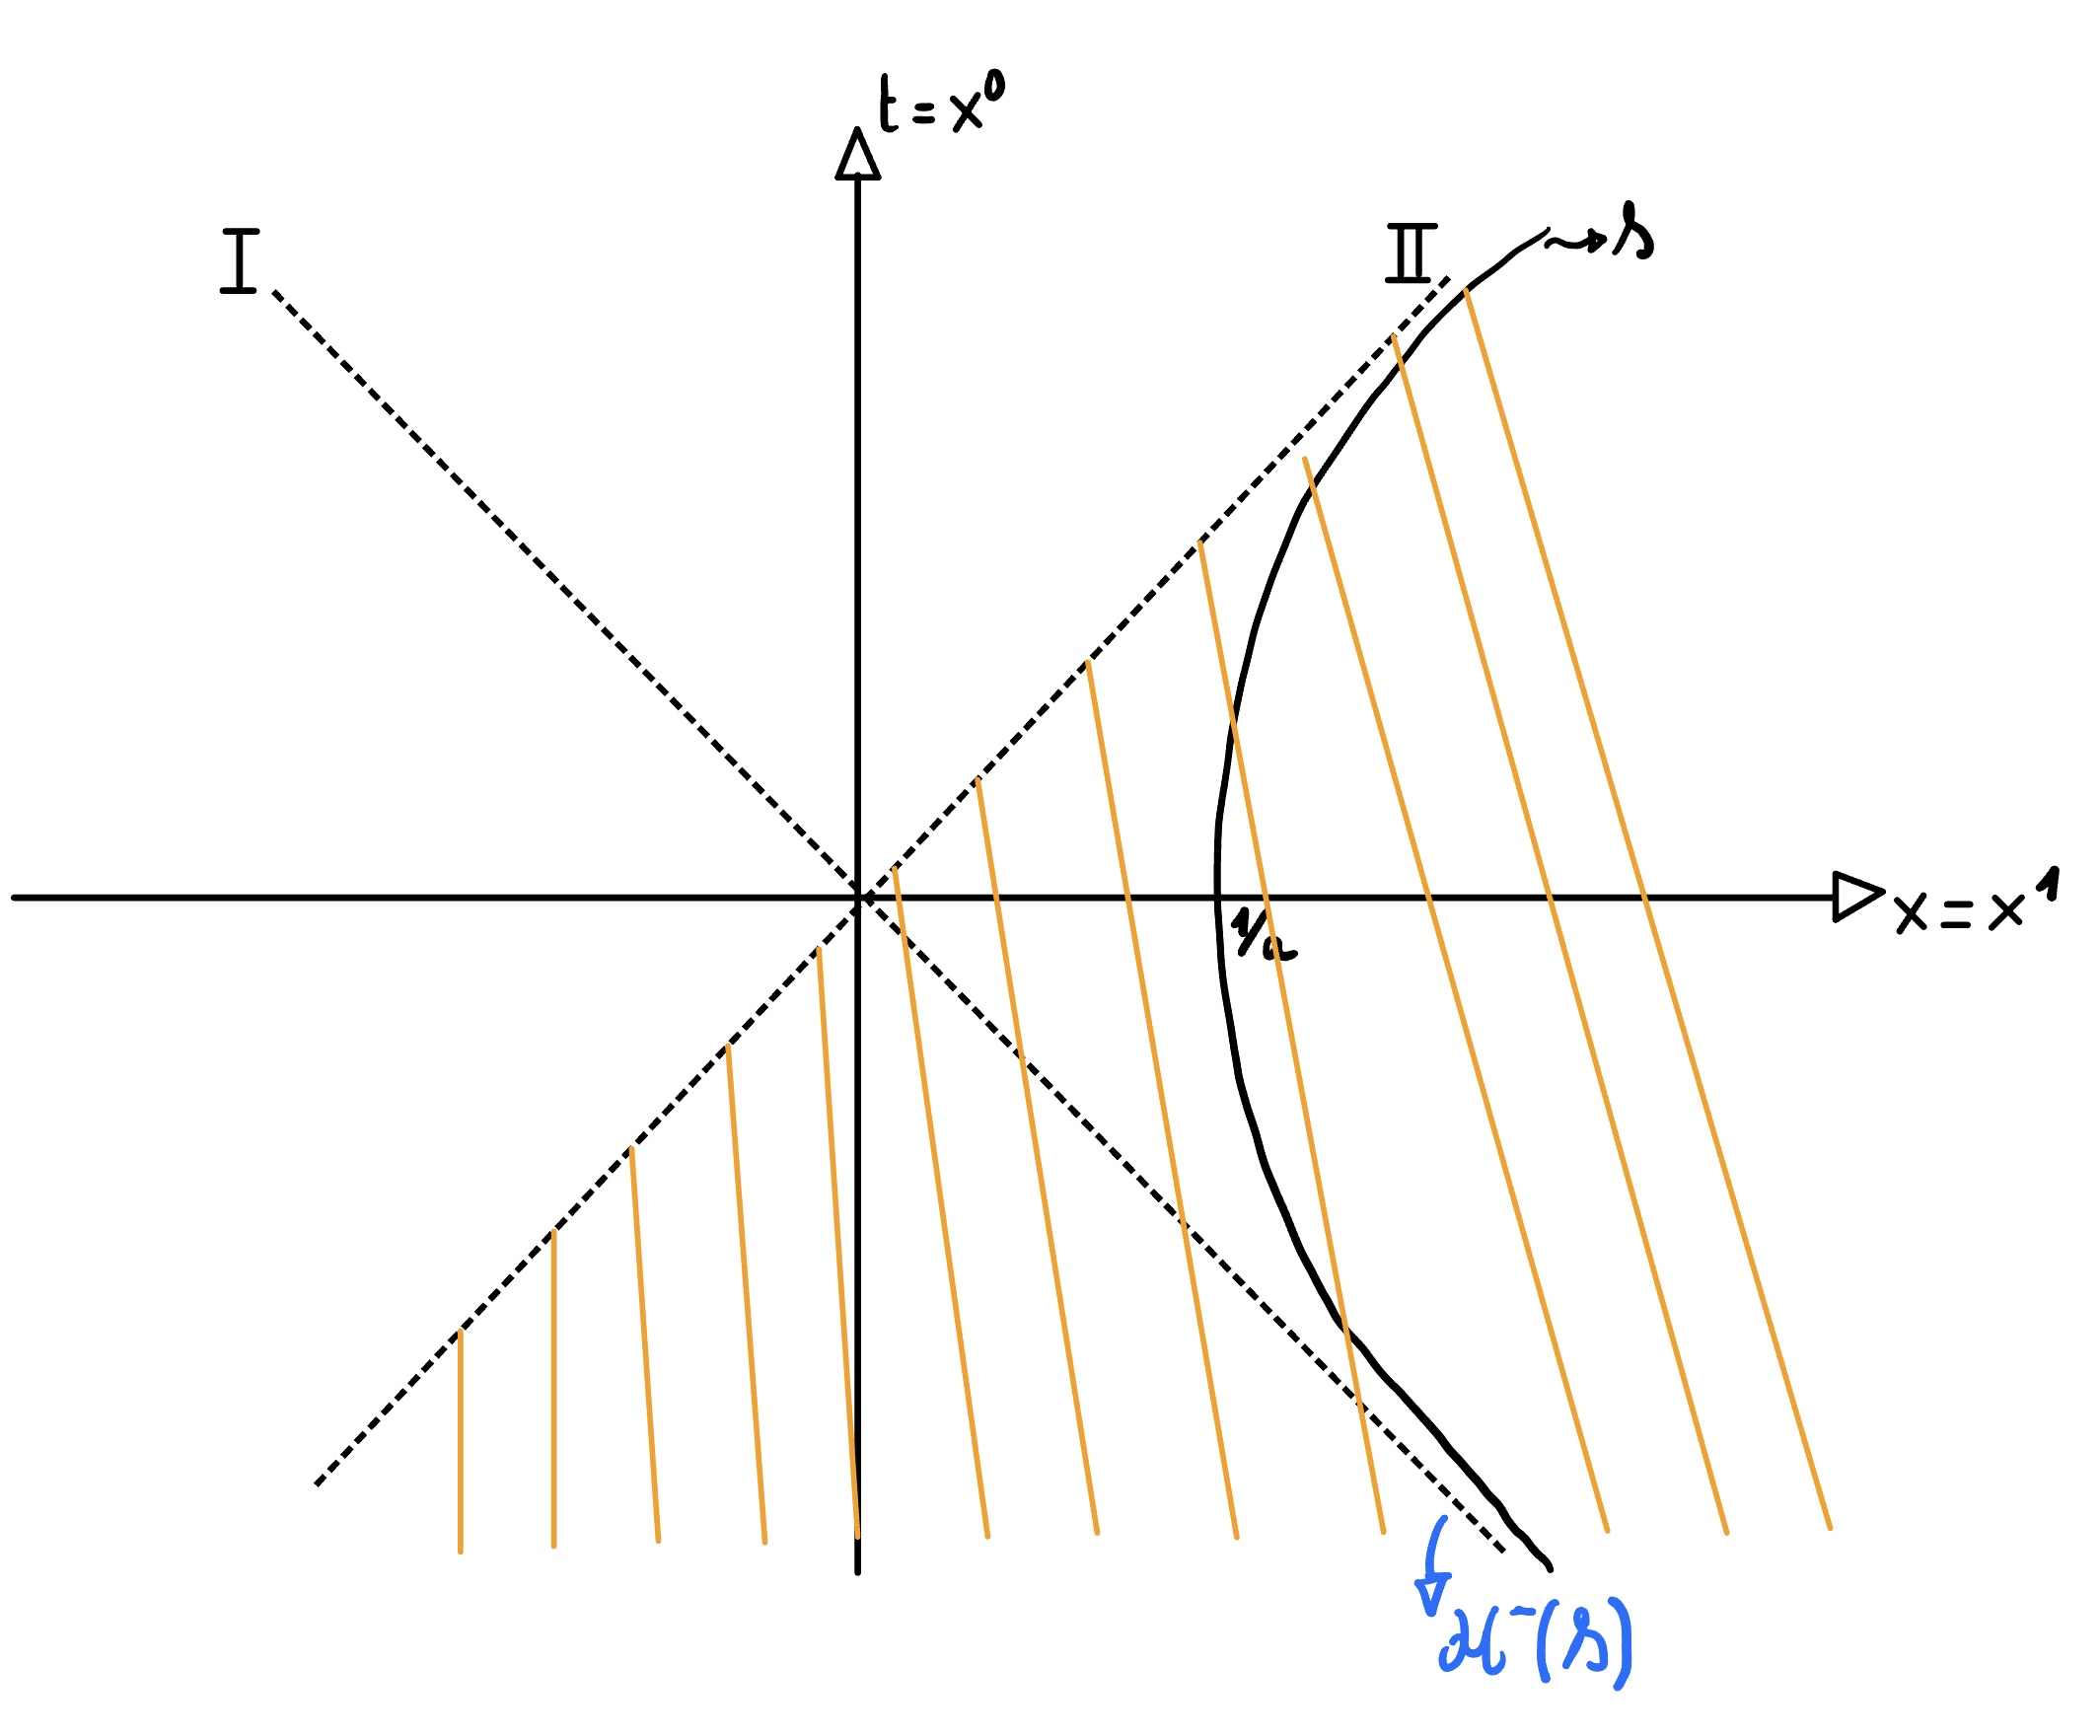
\includegraphics[scale=0.1]{Chapitres/2. Relativité Restreinte/Images/Courbe hyperbole 2.jpg}
\label{Parabolique 2}
\end{center}

$\cRM{1}^{-}(\mathcal{S})$ est une zone où la trajectoire $\mathcal{S}$ peut être affecté par les événements qui ont lieu dans la zone hachurée pour la graphique \ref{Parabolique 2}. 

La frontière de $\cRM{1}^{-}(\mathcal{S})$ est l'horizon des événements futur  de $\mathcal{S}$. Qu'on note $\mathcal{H}^{-}(\mathcal{S})$.

\end{exmp}

\section{Hypersurfaces de Cauchy}
La notion d'hypersurface de Cauchy est importante afin que les problèmes aux limites est bien posé\footnote{Selon Hadamard :)}.

\begin{theoremframe}
    \begin{defi}
        Le \textit{domaine de dépendance future} (ou \textit{développement futur}) d'une région $\mathcal{S}$ de l'espace-temps est l'ensemble des points $P \in \R^{1,3}$ tels que toute courbe causale passant par $P$ intersecte $\mathcal{S}$. Il est noté $\mathcal{D}^+(\mathcal{S})$.
    \end{defi}
\end{theoremframe}
\begin{exmp}
    Soit ???? wtf ?????
\end{exmp}













\chapter{Éléments de géométrie différentielle}

\section{Une première approche heuristique}
Nous développerons lors de ce chapitres les bases nécessaires pour étudier la géométrie d'un espace-temps courbe. Formellement, ceci nécessite d'une connaissance de topologie, et un lecteur intéressé est invité à se renseigner sur le sujet. Pour des raisons pégagogiques, nous allons omettre une définition mathématiquement rigoureuse (via les espaces topologiques de Hausdorff). \\
\\
L'étude d'un espace courbe pose problème : il ne s'agit plus d'un espace vectoriel. Ceci aura comme conséquence que la notion de vecteur perd sa caractéristique globale : nous ne pourrons plus comparer deux vecteurs qui se situent à des points lointains. Cette première section servira à introduire de manière heuristique (c'est-à-dire, avant de définir ce qu'est une variété différentielle). La deuxième section introduira cette notion à proprement dit et retouchera sur les notions de vecteurs. Nous consacrerons ensuite quelques pages pour discuter des p-formes différentielles.
\subsection{Espace tangent}
On se place encore dans l'espace-temps de Minkowski $\mathcal{M}= \R^{1,3}$ avant de généraliser les concepts à une variété différentielle arbitraire.

\begin{theoremframe}
    \begin{notat}
    Soit $P\in \mathcal{M}$. L'espace tangent à $\mathcal{M}$ au point $P$ est noté $T_p\mathcal{M}$. C'est un espace vectoriel réel de dimension 4.
    \end{notat}
\end{theoremframe}
La définition précise d'un espace tangent sera donné ultérieurement. Les éléments de $T_p\mathcal{M}$ sont appelés \textit{vecteurs} au point $P$. 
\begin{rmk}
La notion locale (au point $P$) de cette définition est importante: un vecteur ne pourra pas être vu comme une flèche rejoignant le point $P$ à un autre point $Q \in \mathcal{M}$. Le vecteur \textit{ne vit pas} sur le même espace que les points $P$ et $Q$. Lorsque $\mathcal{M} = \R^{1,3}$, il n'y a pas de problème car les ensembles $\mathcal{M}$ et $T_p\mathcal{M}$ coincident. On peut alors les voir comme des flèches rejoignant deux points distincts. Ceci n'est plus le cas si l'espace-temps est courbe.
\end{rmk}
\begin{theoremframe}
\begin{defi}
    L'union disjointe de tous les espaces tangents de $\mathcal{M}$ noté $T\mathcal{M}=\bigsqcup_P T_p\mathcal{M}$ est appelé \textit{fibré tangent} de $\mathcal{M}$.
\end{defi}
\end{theoremframe}
Comme $T_p\mathcal{M}$ est un espace vectoriel à 4 dimensions, il existe une base de vecteurs $\{\overline{e}_\alpha\}_\alpha$ de $T_p\mathcal{M}$ où $\alpha = \{0,1,2,3\}$. Un vecteur $V \in T_p\mathcal{M}$ peut donc être décomposé sur cette base selon $V = V^\alpha \overline{e}_\alpha$, où $V^\alpha$ sont les composantes du vecteur $V$. Remarquons donc que bien que $V$ ne dépend pas du choix de la base, $V^\alpha$, quant à lui, dépend bien de ce choix.

La donnée d'un vecteur $x_{P} \in T_{p}\mathcal{M}$ à tout $P$ de l'espace est un champ de vecteurs.

Un ensemble canonique de vecteur de $\mathcal{M}$ est un vecteur tangent à une courbe. 

\begin{theoremframe}
    \begin{defi}
        Soit une courbe lisse $\R \to \mathcal{M}: \lambda \mapsto x^\mu (\lambda)$. Le vecteur tangent à la courbe est
        \begin{equation}
            V^\alpha = \frac{\td x^\alpha}{\td \lambda}
        \end{equation}
    \end{defi}
\end{theoremframe}
\begin{theoremframe}
\begin{propri}
    Soit un vecteur $V^\alpha\in T_p\mathcal{M}$. Sous transformation de Poincaré, ce vecteur se transforme comme
    \begin{equation}
        V^{\alpha'} = \Lambda^{\alpha'}_{\; \mu} V^\mu
    \end{equation}
\end{propri}
\end{theoremframe}
\begin{proof}
    Soit une courbe lisse $x^\mu(\lambda)$. Sous transformation de Poincaré, cette courbe se transforme comme $x^{\mu'} = \Lambda^{\mu'}_{\; \mu} x^\mu + a^{\mu'}$. Notons $V^\mu$ le vecteur tangent à la courbe au point $P$. Alors, par définition de $V$, on trouve
    \begin{align}
        V^{\mu'} = \frac{\td x^{\mu'}}{\td \lambda} = \Lambda^{\mu'}_{\; \mu} \frac{\td x^{\mu}}{\td \lambda} = \Lambda^{\mu'}_{\; \mu} V^\mu
    \end{align}
\end{proof}
\begin{theoremframe}
    \begin{propri}
        Sous transformation de Poincaré, les vecteurs de base se transforment comme
        \begin{equation}
            \overline{e}_{\mu '} = \Lambda^{\cdot\,\mu}_{\mu'}\overline{e}_{\mu}
        \end{equation}
    \end{propri}
\end{theoremframe}
\begin{proof}
La décomposition d'un vecteur dans deux référentiels inertiels différents s'écrit
    \begin{equation}
    V = V^{\mu} \overline{e}_{\mu} = V^{\alpha '} \overline{e}_{\alpha '}
\end{equation}
Ainsi,
\begin{equation}
    V^{\alpha '} \overline{e}_{\alpha '} = \Lambda^{\alpha'}_{\; \mu} V^\mu \overline{e}_{\alpha '} = V^\mu \overline{e}_{\mu}
\end{equation}
Comme ceci est valable pour $V^\mu$ arbitraire, on conclut que 
\begin{equation}
    \Lambda^{\alpha'}_{\; \mu} \overline{e}_{\alpha '} = \overline{e}_{\mu}.
\end{equation}
En remarquant que $\Lambda$ vérifie
\begin{equation}
    \Lambda^\alpha_{\;\mu} \eta_{\alpha\beta} \Lambda^\beta_{\;\nu} = \eta_{\mu\nu}
\end{equation}
on trouve la propriété
\begin{equation}
    \label{eq:id lambda}
    \Lambda^\alpha_{\;\mu} \Lambda^{\cdot\,\nu}_\alpha = \delta^{\cdot\, \nu}_\mu
\end{equation}
où le point clarifie l'ordre des indices. Ceci permet de conclure, en multipliant par $\Lambda^{\cdot\,\nu}_\alpha$ que
\begin{equation}
    \overline{e}_{\alpha '} = \Lambda^{\cdot\,\mu}_{\alpha'}\overline{e}_{\mu}
\end{equation}
\end{proof}

\subsection{Espace co-tangent}
\begin{theoremframe}
    \begin{defi}
        Une forme linéaire sur un espace vectoriel $(\mathcal{V},\mathbb{K})$ est une application linéaire $w:\mathcal{V} \to \mathbb{K}$. Pour $a,b\in \mathbb{K}$ et $X,Y \in \mathcal{V}$, on a donc
        \begin{equation}
            w(aX+bY) = aw(X)+bw(y)
        \end{equation}
    \end{defi}
\end{theoremframe}
Nous appelons \textit{dual} d'un espace vectoriel $V$ l'ensemble des formes linéaires sur cet espace.
\begin{theoremframe}
    \begin{defi}
        L'espace \textit{co-tangent} à $\mathcal{M}$ en un point $P$ est le dual de $T_p\mathcal{M}$ et est noté $T_p^*\mathcal{M} = (T_p\mathcal{M)^*}$.
    \end{defi}
\end{theoremframe}
\begin{theoremframe}
    \begin{defi}
        Un \textit{covecteur} est un élément de l'espace co-tangent $w\in T_p^*\mathcal{M}$.
    \end{defi}
\end{theoremframe}
On peut définir une base $\{\Theta^\mu\}_\mu$ sur l'espace co-tangent selon l'identité
\begin{equation}
    \Theta^\mu(\overline{e}_\nu)=\delta^\mu_\nu
\end{equation}
Dans cette base, un covecteur $w\in T_p^*\mathcal{M}$ s'écrit $w = w_\alpha \theta^\alpha$. Soit $V \in T_p\mathcal{M}$:
\begin{align}
    w(V) &= w_{\alpha} \Theta^{\alpha}(V^{\mu} \Vec{e_{\mu}})\\
    &=w_{\alpha} V^{\mu}\Theta^{\alpha} (\Vec{e_{\mu})}\\
    &= w_{\alpha} V^{\mu}\delta^{\alpha}_{\mu}\\
    &= w_{\alpha} V^{\alpha} \in \R
\end{align}


où $V$ est un vecteur de l'espace tangent. 

Cette expression ne dépend pas du choix de base. De plus, elle ne comporte pas d'indices libres. Un tel terme est appelé scalaire de Lorentz. On peut l'écrire de manière équivalente comme $w(V) = w_{\alpha} V^{\alpha} = w_{\alpha '} V^{\alpha '} $.
\begin{rmk}
    Dans un espace vectoriel de dimension finie, le dual de l'espace dual est identifié à $T_p\mathcal{M}$. On a donc $(T^*_P\mathcal{M})^* = T_p\mathcal{M}$.
\end{rmk} 
\begin{theoremframe}
    \begin{propri}
        Soit un covecteur $V^\alpha\in T^*_P\mathcal{M}$. Sous transformation de Poincaré, ce covecteur se transforme comme
    \begin{align}
        w_{\alpha'} = \Lambda^{\cdot \, \mu}_{\alpha'} V^\mu
    \end{align}
    \end{propri}
\end{theoremframe}
\begin{proof}
    On vient de voir que $w(V)$ est un scalaire de Lorentz:
    \begin{equation}
        w(V) = w_{\alpha} V^{\alpha} = w_{\alpha '} V^{\alpha '} 
    \end{equation}
    Et donc par la loi de transformation d'un vecteur, on a
    \begin{equation}
        w_{\alpha} V^{\alpha} = w_{\alpha '} \Lambda^{\alpha '}_{\;\mu} V^\mu
    \end{equation}
    Comme ceci est valable pour tout vecteur $V$, on peut écrire
    \begin{equation}
        w_{\alpha}  = w_{\alpha '} \Lambda^{\alpha '}_{\;\alpha}
    \end{equation}
    Et on trouve le résultat recherché en utilisant l'identité \ref{eq:id lambda}.
\end{proof}

En particulier, la base de l'espace co-tangent se transforme comme:
$$ \Theta^{\alpha '} = \Lambda^{\alpha '}_{\; \mu} \Theta^{\mu}$$

\begin{theoremframe}
    \begin{defi}
        L'union de tous les espaces co-tangents de $\mathcal{M}$ noté $\bigcup_P T^*_P\mathcal{M}$ est appelé \textit{fibré co-tangent} de $\mathcal{M}$.
    \end{defi}
\end{theoremframe}
Maintenant qu'on a explicité l'emplacement des indices corrects, nous n'allons plus l'indiquer pour le reste de ce syllabus afin de simplifier les notations.

\subsection{Les tenseurs}

On peut généraliser les notions de vecteur et covecteur à un tenseur. Si on considère un vecteur $V \in T_{p}\mathcal{M} : T^*_{p}\mathcal{M} \rightarrow \mathbb{R}$ et un covecteur $w \in T^*_{p}\mathcal{M} : T_{p}\mathcal{M} \rightarrow \mathbb{R}$, alors on peut voir le vecteur $V$ comme un tenseur $(1, 0)$ et on peut voir le covecteur $w$ comme un tenseur $(0, 1)$. 
\begin{theoremframe}
    \begin{defi}
        Un tenseur de type $(k, l)$ au point $P$ est une application multilinéaire
        \begin{equation}
            \underbrace{T^*_{p}\mathcal{M} \times \cdots \times T^*_{p}\mathcal{M}}_\text{$k$-fois} \times \underbrace{T_{p}\mathcal{M} \times \cdots \times T_{p}\mathcal{M}}_\text{$l$-fois}  \to \mathbb{R}
        \end{equation}

        Multilinéaire signifie linéarité en chaque variable, donc par exemple pour un tenseur de type $(1,1)$: 
        \begin{equation}
        T(aw +b\eta, cX +dY) = acT(w, X) + adT(w, Y) + bcT(\eta, X) +cdT(\eta, Y)
        \end{equation}
        où $a,b, c ,d \in \mathbb{R}$
    \end{defi}
\end{theoremframe}
\begin{exmp}
    Un tenseur $(1, 1)$ est tel que $T(w,V) \in \R$ où $w$ est un covecteur et $V$ est un vecteur. 
\end{exmp}
\begin{exmp}
    Si un tenseur $T$ est tel que pour $V\in T_p\mathcal{M}$, on a $T(V) \in T^*_p\mathcal{M}$, alors il s'agit d'un tenseur de type (0,2).
\end{exmp}
\begin{theoremframe}
    \begin{propri}
        L'ensemble des tenseurs de type $(k, l)$ en $P\in \mathcal{M}$ forment un espace vectoriel. Une base de cette espace vectoriel est donnée par 
        \begin{equation}
        \overline{e}_{\alpha_1} \otimes \cdots \otimes \overline{e}_{\alpha_k} \otimes \Theta^{\mu _1}\otimes \cdots \otimes \Theta^{\mu _l}
        \end{equation}
    \end{propri}
\end{theoremframe}
Un tenseur de type $(k,l)$ se décompose donc sur cette base comme
\begin{equation}
    T = T\indices{^{\alpha _1 \cdots \alpha _k}_{v_1 \cdots v_l}}\overline{e}_{\alpha_1} \otimes \cdots \otimes \overline{e}_{\alpha_k} \otimes \Theta^{v _1}\otimes \cdots \otimes \Theta^{v _l}
\end{equation}
\begin{theoremframe}
    \begin{propri}
        Un vecteur de type $(k,l)$ se transforme sous transformation de Poincaré comme\footnote{Ici, $\times$ est utilisé pour la multiplication usuelle et non comme produit direct.}
        \begin{equation}
            T\indices{^{\alpha ' _1 \cdots \alpha ' _k}_{v'_1 \cdots v'_l}} = \Lambda\indices{^{\alpha '_1}_{\alpha _1 }} \times \cdots \times \Lambda\indices{^{\alpha '_k}_{\alpha _k}} \times \Lambda\indices{_{v'_1 }^{v_1 }} \times \cdots \times \Lambda\indices{_{v'_k}^{v_k}} \times T\indices{^{\alpha _1 \cdots \alpha _k}_{v_1 \cdots v_l}}.
        \end{equation}
        La transformation implique donc $k+l$ matrices de Lorentz.
    \end{propri}
\end{theoremframe}
\begin{proof}
    Conséquence des propriétés précédentes.
\end{proof}

Revenons à la métrique de Minkowski. Celle-ci peut-être vue comme un tenseur $(2.0)$ symétrique.
\begin{equation*}
    \eta_{\mu ' \nu '} = \Lambda\indices{_{\mu '}^{\alpha}}\Lambda\indices{_{\nu ' }^{\beta}}\eta_{\alpha \beta}
\end{equation*}
De plus, la métrique de Minkowski est un invariant de Lorentz. Donc elle a les mêmes coordonnées dans tout référentiel inertiel.

\begin{theoremframe}
    \begin{defi}
        La métrique de Minkowski est un pseudo-produit scalaire pour l'espace $T_p\mathcal{M}$. En effet, celle-ci est une forme linéaire 
        \begin{align}
        \eta:\begin{pmatrix}
             T_p\mathcal{M} \times T_p\mathcal{M} & \to & \R\\
            (X,Y) & \mapsto & \eta(X,Y) = \eta_{\mu  \nu }X^{\mu}Y^{\nu}
        \end{pmatrix}
        \end{align}.
        En particulier, $\eta$ est symétrique et biliéaire.
    \end{defi}
    
\end{theoremframe}
\begin{rmk}
    Elle définit un pseudo-produit scalaire car elle n'est ni définie positive $\eta(X,X) \ngeq 0$, ni sépare les points $\eta(X,X) = 0 \centernot \implies X = 0$.
\end{rmk}
On dira que deux vecteurs sont orthogonaux si et seulement si $\eta (X, Y) = 0$. On note la norme d'un vecteur

\begin{align*}
    \lVert V \rVert ^2 = \eta (V, V) = \left\{
\begin{array}{l}
  < 0 \text{ si } V \text{est de genre temps} \\
  > 0 \text{ si } V \text{est de genre espace}\\
  = 0 \text{ si } V \text{est de genre lumière}
\end{array}
\right.
\end{align*}

La métrique permet d'établir un isomorphisme entre $T_{p}\mathcal{M} $ et $T^*_{p}\mathcal{M}$. C'est-à-dire qu'il permet d'associer un vecteur à un covecteur tel que

\begin{align*}
    \eta : \begin{pmatrix}
        T_{p}\mathcal{M} &\to & T^*_{p}\mathcal{M}\\
             V &\mapsto &\eta (V, \cdot)
    \end{pmatrix}
\end{align*}
Ceci justifie la convention que $\eta$ permet de monter ou descendre les indices tel que:

\begin{equation*}
    V^{\mu} \rightarrow \eta_{\mu \nu}V^{\mu} \equiv V_{\nu}
\end{equation*}

Donc par définition, l'espace temps de Minkowski est l'espace temps plat muni de la métrique de Minkowski. 

\subsection{Avantage de la notation tensorielle}
Outre le fait que la notation tensorielle permet une formulation plus compacte, on a également le résultat suivant:
\begin{theoremframe}
    \begin{prop}
        Si une relation tensorielle est valable dans un référentiel interiel alors elle sera valable dans tout référentiel inertiel.
    \end{prop}
\end{theoremframe}

Illustrons cette propriété avec les équations de Maxwell. Les équations de Maxwell sont des invariants de Lorentz mais c'est compliqué de le montrer explicitement (surtout pour les boosts). Une manière plus simple de le montrer est de les écrire en notation tensorielle, dans lesquelles elles seront nécessairement invariantes.

Les équations de Maxwell sont:

$$\left\{
\begin{array}{l}
  \vect{\nabla} \times \vect{B} -\partial_{t} \vect{E} = \vect{J}  \\
  \vect{\nabla} \cdot \vect{E} = \rho\\
  \vect{\nabla} \cdot \vect{B} = 0\\
  \vect{\nabla} \times \partial_t \vect{B} = \vect{0}
\end{array}
\right.$$

Pour écrire ces équations de manière tensorielle, on va définir le tenseur de Faraday (le tenseur de Faraday dépend du signe de la métrique ):


\begin{align}
\label{eq: Faraday}
 F_{\mu \nu}^{(-+++)} =  \begin{pmatrix}
0 & -E_1 & -E_2 & -E_3\\
E_1 & 0 & B_3 & -B_2\\
E_2 & -B_3 & 0 & B_1\\
E_3 & B_2 & -B_1 & 0\\
\end{pmatrix}   
\end{align}

Ce tenseur est antisymétrique $F_{\mu \nu}^{(-+++)} = - F_{\nu \mu}^{(-+++)}$

On peut réécrire les équations de Maxwell comme:

$$\left\{
\begin{array}{l}
  \partial_{\mu} F^{\mu \nu} = J^{\nu}(x) \\
  \partial_{[{\alpha}}F_{\mu \nu]} = 0(t)
\end{array}
\right.$$

où $J^{\mu} = (\rho, \Vec{J})$ est le quadri-courant.

La notation entre crochet est appelée anti-symétrisation et est défini par

\begin{equation}
    T_{[\mu_{1}, ... , \mu_{n}]} =\frac{1}{n!}(T_{\mu_{1}, ... , \mu_{n}} + \text{permutations signées des n indices})
\end{equation}

qui possède posséde $n!$ termes. 

\begin{exmp}
    \begin{equation*}
        T_{[\alpha \beta]} = \frac{1}{2!}\left(T_{\alpha\beta} - T_{ \beta \alpha}\right)
    \end{equation*}
\end{exmp}


On va montrer que la loi de Gauss peut s'écrire manière tensorielle.
On sait que la loi de Gauss est:

\begin{equation}
    \Vec{\nabla}\cdot \Vec{E} = \rho
\end{equation}
soit
\begin{equation}
    \partial_{i}E^{i} = J^{0}
    \label{loi de Gauss}
\end{equation}
\begin{rmk}
     On peut monter et descendre les indices spatiales sans conséquences $E^{i} = \eta^{ij}E_{j} = E_{i}$.
\end{rmk}

Par définition du tenseur de Faraday, on a
\begin{equation}
    F_{0i} = -E_i \text{ car } F_{01} = -E_1
\end{equation}
Remarquons que alors

\begin{equation}
    F^{0i} = \eta ^{0 \alpha} \eta ^{i\beta} F_{\alpha \beta} = (-)(+1)F_{0i} = -F_{0i} = E_j
    \label{Faraday}
\end{equation}

Donc en remplaçant le résultat \ref{Faraday} dans l'équation \ref{loi de Gauss}, on obtient:

\begin{equation}
    \partial_{i}F^{0i} = J^0
    \label{Loi de Gauss tensoirel}
\end{equation}

Comme $F^{\mu \nu}$ est antisymétrique, on a que $F^{00} = 0$. Donc on peut réécrire \ref{Loi de Gauss tensoirel} comme,

\begin{equation}
    \partial_{\alpha}F^{0\alpha} = J^0
\end{equation}

De manière similaire, il est possible d'intégrer la loi d'Ampère pour donner

\begin{equation}
    \label{eq:faraday tot}
    \partial_{\mu}F^{\mu\nu} = J^{\nu}
\end{equation}

Montrons que cette expression ne dépend effectivement pas du référentiel inertiel choisi. On sait que $x'^{\mu} = \Lambda^{\mu'}_{\alpha}x^{\alpha}$.
Donc on a que \ref{eq:faraday tot} peut se réécrire comme:

\begin{equation}
   \Lambda^{\nu '}_{\mu} \partial_{\nu '}(\Lambda ^{\mu}_{\alpha'}\Lambda ^{\nu}_{\beta '}F^{\alpha ' \beta '} ) =  \Lambda^{\nu }_{\alpha'}J^{\alpha '}
\end{equation}
par la loi de transformation tensorielle. Comme les matrices $\Lambda ^{\mu}_{\alpha'}$ et $\Lambda ^{\nu}_{\beta '}$ sont constantes, on peut les sortir de la dérivée. 

\begin{align}
   \overbrace{\Lambda^{\nu '}_{\mu} \Lambda ^{\mu}_{\alpha'}}^{\displaystyle\delta^{\nu '}_{\alpha' }}\Lambda ^{\nu}_{\beta '} \partial_{\nu '} F^{\alpha ' \beta '} & =  \Lambda^{\nu }_{\alpha'}J^{\alpha '} \\
   \implies \Lambda ^{\nu}_{\beta '} \partial_{\nu '} F^{\nu ' \beta '}  &=  \Lambda^{\nu }_{\alpha'}J^{\alpha '}
\end{align}

Et en multipliant des deux côtés par $\displaystyle\Lambda^\gamma_\nu$, on obtient bien

\begin{equation}
    \partial_{\alpha '}F^{\alpha ' \gamma '} = J^{\gamma '}
\end{equation}

Ceci montre bien que dans l'exemple des lois de Maxwell, l'expression tensorielle dans un système inertiel est en fait valable pour tout référentiel.

\section{Variétés différentielles}
Nous allons à présent considérer un espace-temps $\mathcal{M}$ avec courbure. Pour ce, il est utile d'introduire la notion de variété différentielle. Avant de voir celle-ci, nous rappellerons quelques notions de topologie.
\begin{theoremframe}
    \begin{defi}
        Soit $X$, un ensemble non-vide. Une collection $\mathcal{T}_X$ de sous-ensembles de $X$ est une \textit{topologie sur $X$} si
        \begin{itemize}
            \item[(i).] $X,\empty \in \mathcal{T}_X$.
            \item[(ii).] Si $U_1,\cdots,U_k \in \mathcal{T}_X$, alors $U_1 \cap \cdots \cap U_k \in \mathcal{T}_X$.
            \item[(iii).] Si $\{ U_i\}_{i\in I}$ est une collection quelconque d'éléments de $\mathcal{T}_X$, alors $\bigcup_{i\in I} U_i \in \mathcal{T}_X$.
        \end{itemize}
        Le couple $(X,\mathcal{T}_X)$ est un \textit{espace topologique}. Les éléments de $U\in \mathcal{T}_X$ sont les ouverts de l'espace topologique.
    \end{defi}
\end{theoremframe}
Sur base de cette définition, il est possible de reconstruire les notions d'analyse comme la continuité et la différentiabilité comme approche alternative à la notion séquentielle (via des suites). Nous n'allons pas aller en détail dans cette approche et directement passer au sujet de la géométrie différentielle.
\begin{theoremframe}
    \begin{defi}
        Une application sur des ouverts $f:U\to V$ est un \emph{homéomorphisme} si $f:U\to V$ est bijective et $f,f^{-1}$ sont continues. 
    \end{defi}
\end{theoremframe}
Notons que nous considérerons dans la suite que l'homéomorphisme sera lisse (c'est-à-dire $C^\infty$). L'utilité d'un homéomorphisme réside dans le fait qu'il préserve la structure topologique des espaces. Par exemple, Une tasse de café et un donut sont homéomorphes, car l'un peut être transformé en l'autre continûment, sans coupures.
\begin{theoremframe}
    \begin{defi}
        Un \textit{atlas} (lisse) d'un espace topologique $\mathcal{M}$ est une collection de paires $(U_i,\varphi_i) \quad {i\in I}$ telle que :
        \begin{itemize}
            \item[(i).] $\forall i\in I$, $U_i \in \mathcal{T}_\mathcal{M}$ et de plus, $\bigcup_{i\in I} U_i = \mathcal{M}$.
            \item[(ii).] $\varphi_i:U_i\to V_i$ où $V_i$ est un ouvert de $\R^m$ est un homéomorphisme.
            \item[(iii).] Si $U_i \cap U_j \neq \varnothing$, l'application 
            \begin{align}
            \varphi_{ij} = \varphi_i \circ \varphi^{-1}_j:\varphi_j(U_i\cap U_j) \subset \R^m \to \varphi_i(U_i\cap U_j) \subset \R^m 
            \end{align}
            est lisse. Cette fonction est également appelée la fonction de transition.
        \end{itemize}
    \end{defi}
\end{theoremframe}
\begin{theoremframe}
    \begin{defi}
        Une variété différentielle $\mathcal{M}$ de dimension $m$ est un espace topologique muni d'un atlas.
    \end{defi}
\end{theoremframe}
\begin{rmk} 
    \begin{enumerate}
        \item[\,] 
        \item L'application $\varphi_i^{-1}$ est appelée \emph{paramétrisation locale} de $\mathcal{M}$ sur $U_i\in \mathcal{M}$. Elle permet d'associer des coordonnées de $\R^m$ à chaque point de $U_i$. On dira que $\mathcal{M}$ ressemble localement à des ouverts de $\R^m$.
        \begin{figure}[H]
            \centering
            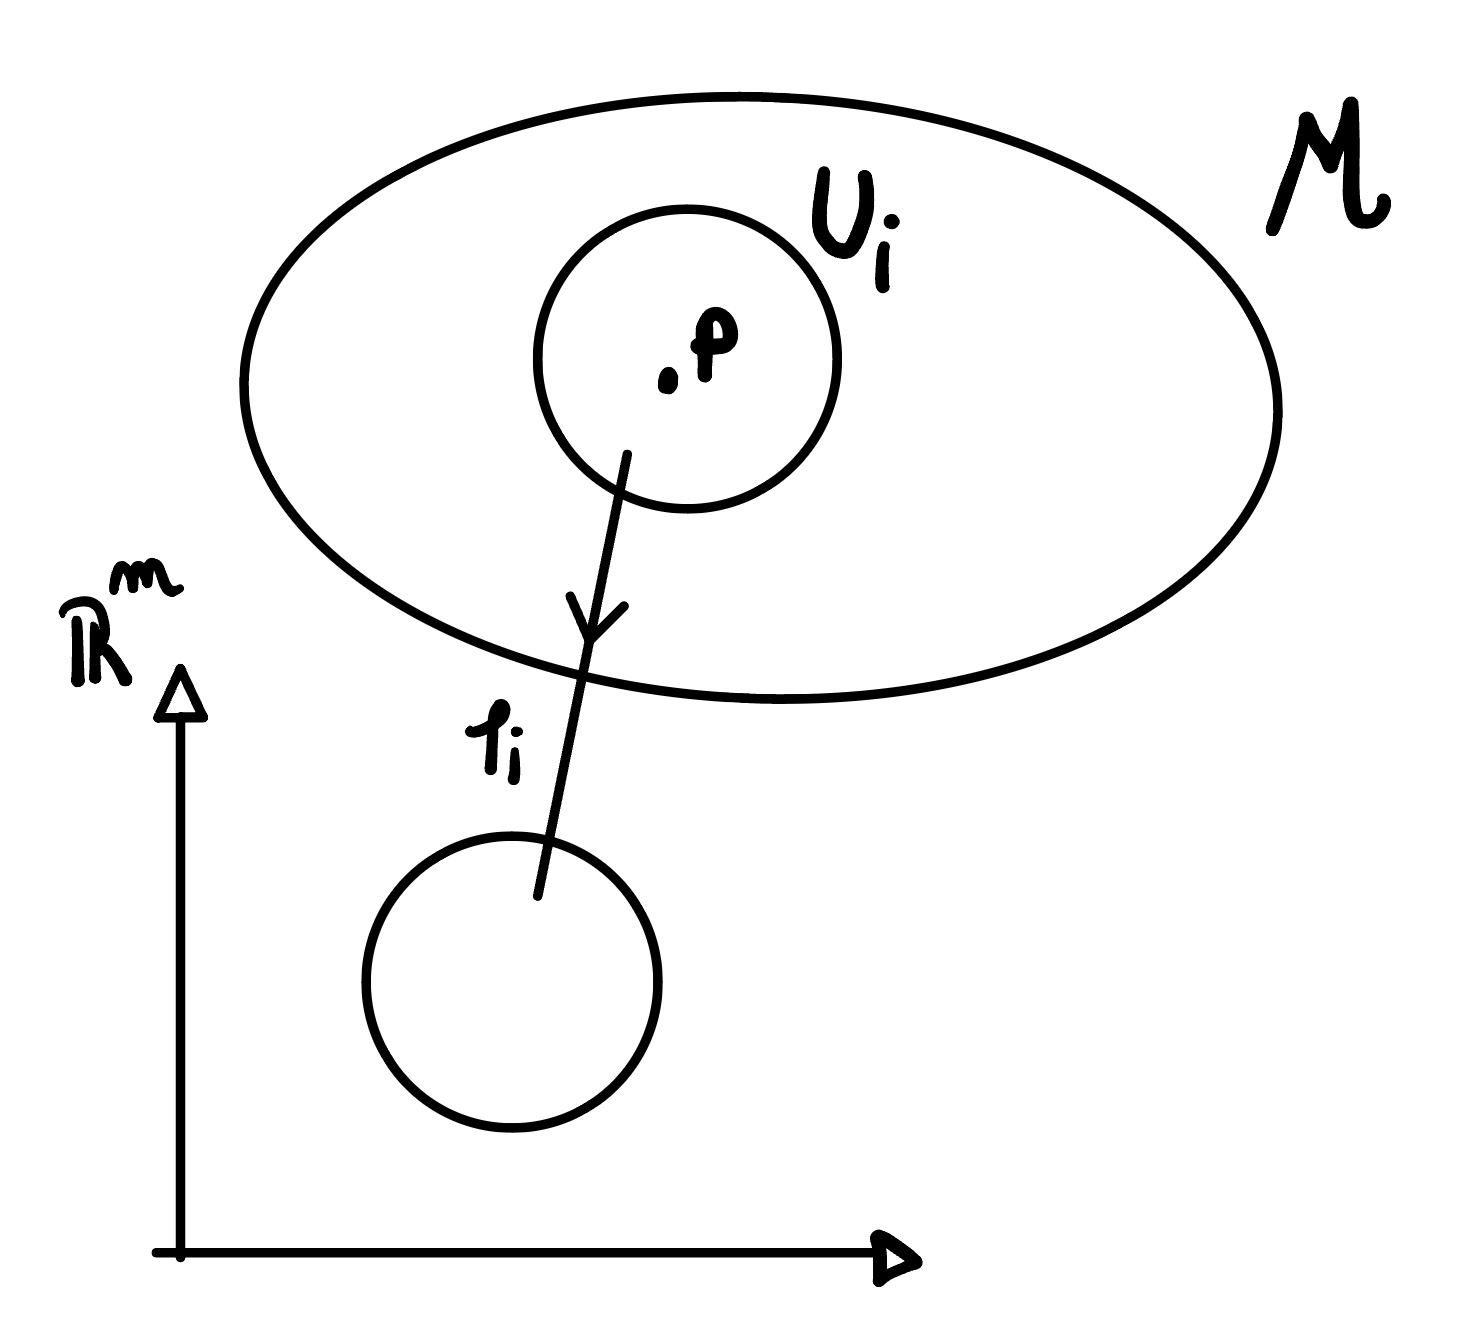
\includegraphics[width=0.3\linewidth]{Chapitres/3.Element de géométrie différentielle/Images/variété.jpg}
            \caption{}
            \label{fig:3.1}
        \end{figure}
        \item La condition (iii). impose que ces morceaux de $\R^m$ peuvent être "recollés" de manière lisse.
        \begin{figure}[H]
            \centering
            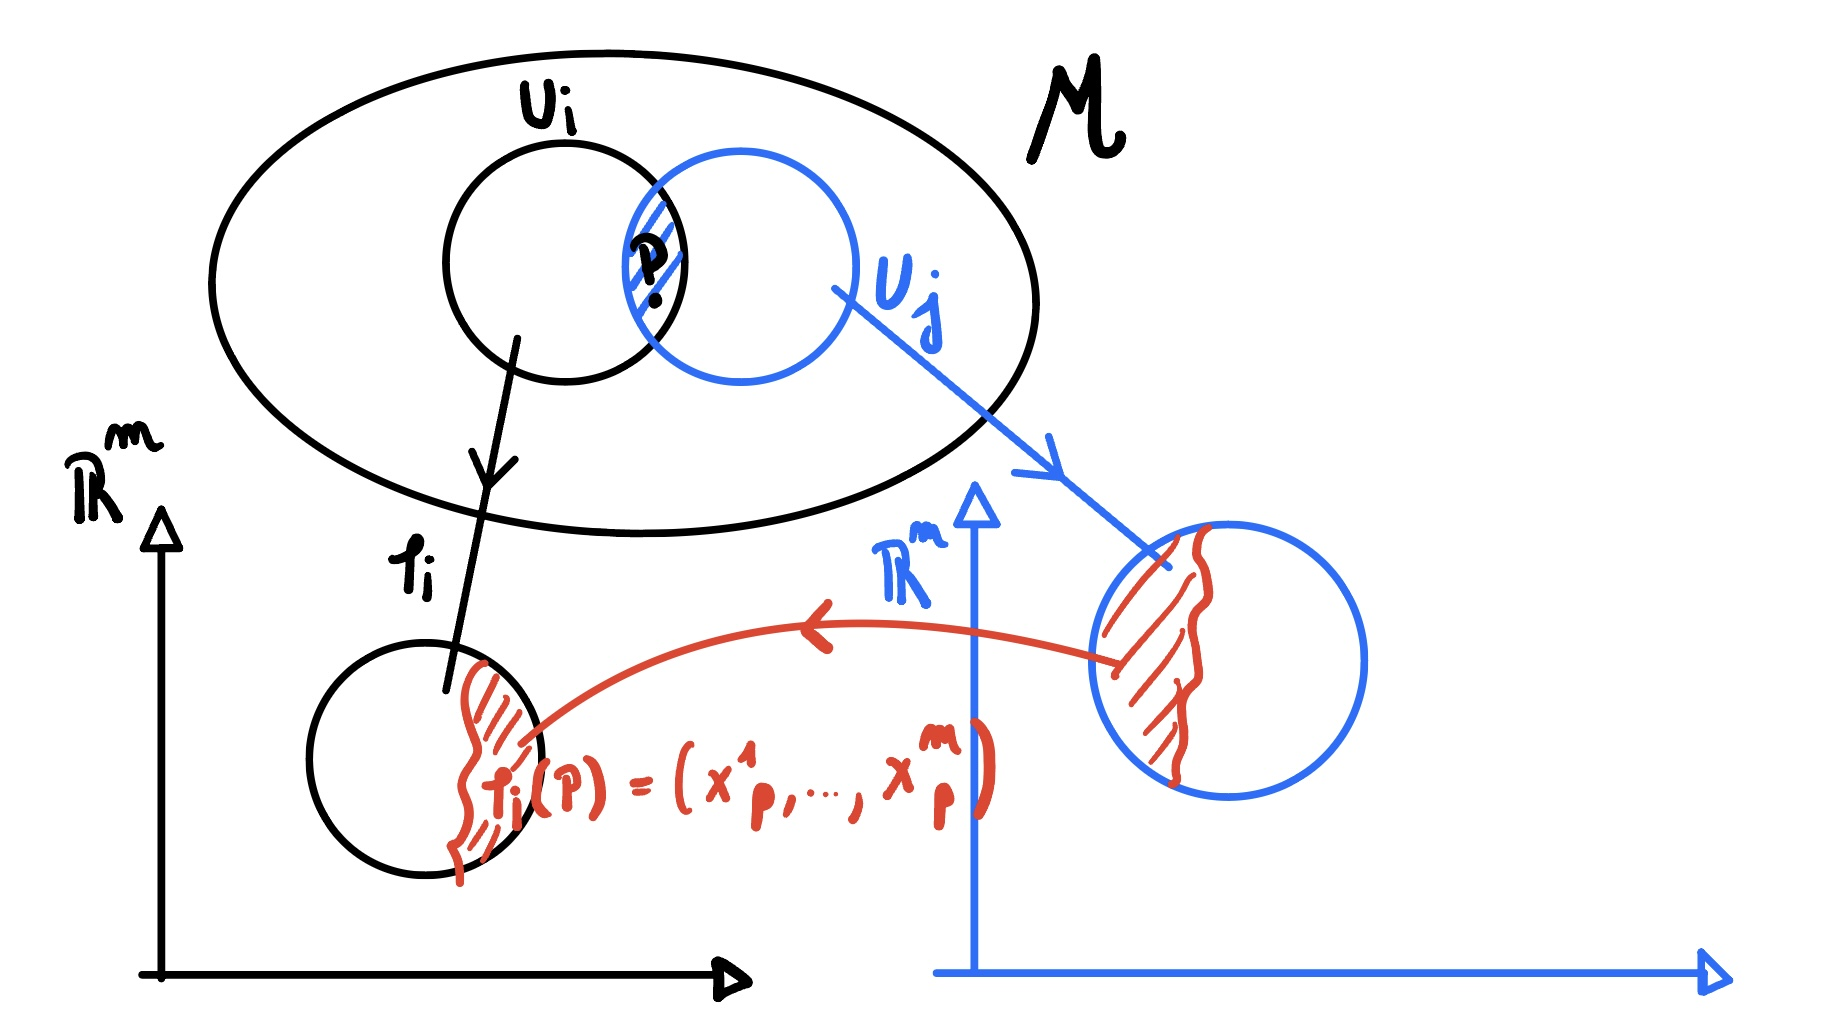
\includegraphics[width=0.5\linewidth]{Chapitres/3.Element de géométrie différentielle/Images/ouvertchevauchement.jpg}
            \caption{Sur les images de l'intersection de $U_i$ et $U_j$, il existe une bijection lisse.}
            \label{fig:3.2}
        \end{figure}
        \item Les atlas sur les variétés ne sont pas uniques. Les différents choix d'atlas correspond aux différents choix physique de système de coordonnées. La liberté de changer d'atlas correspond à la liberté de changer de coordonnées ou de référentiel pour décrire une variété.
    \end{enumerate}
\end{rmk}
    \begin{exerc}
        Montrez qu'un cône n'est pas une variété lisse. Pour rappel, le cône est défini comme 
        \begin{equation}
            C = \ltc (x,y,z)\in \R^3 \mid x^2+y^2-z^2=0, z\geq 0 \rtc
        \end{equation}
    \end{exerc}
\subsection{Application entre variété}
Soient deux variétés différentielles $\mathcal{M}$ et $ \mathcal{N}$ respectivement à cartes locales $(U,\varphi)$ et $(V,\psi)$ et une application continue $f:\mathcal{M} \to \mathcal{N}$.

\begin{theoremframe}
    \begin{defi}
        L'application $f$ est dite \emph{lisse} si et seulement si l'application 
        \begin{equation}
        F = \psi \circ f \circ \varphi^{-1}:\varphi(U) \to \psi(V)
        \end{equation}
        est lisse. Cette fonction est appelée \emph{représentation de coordonnées locales de} $f$.
    \end{defi}
\end{theoremframe}

\begin{center}
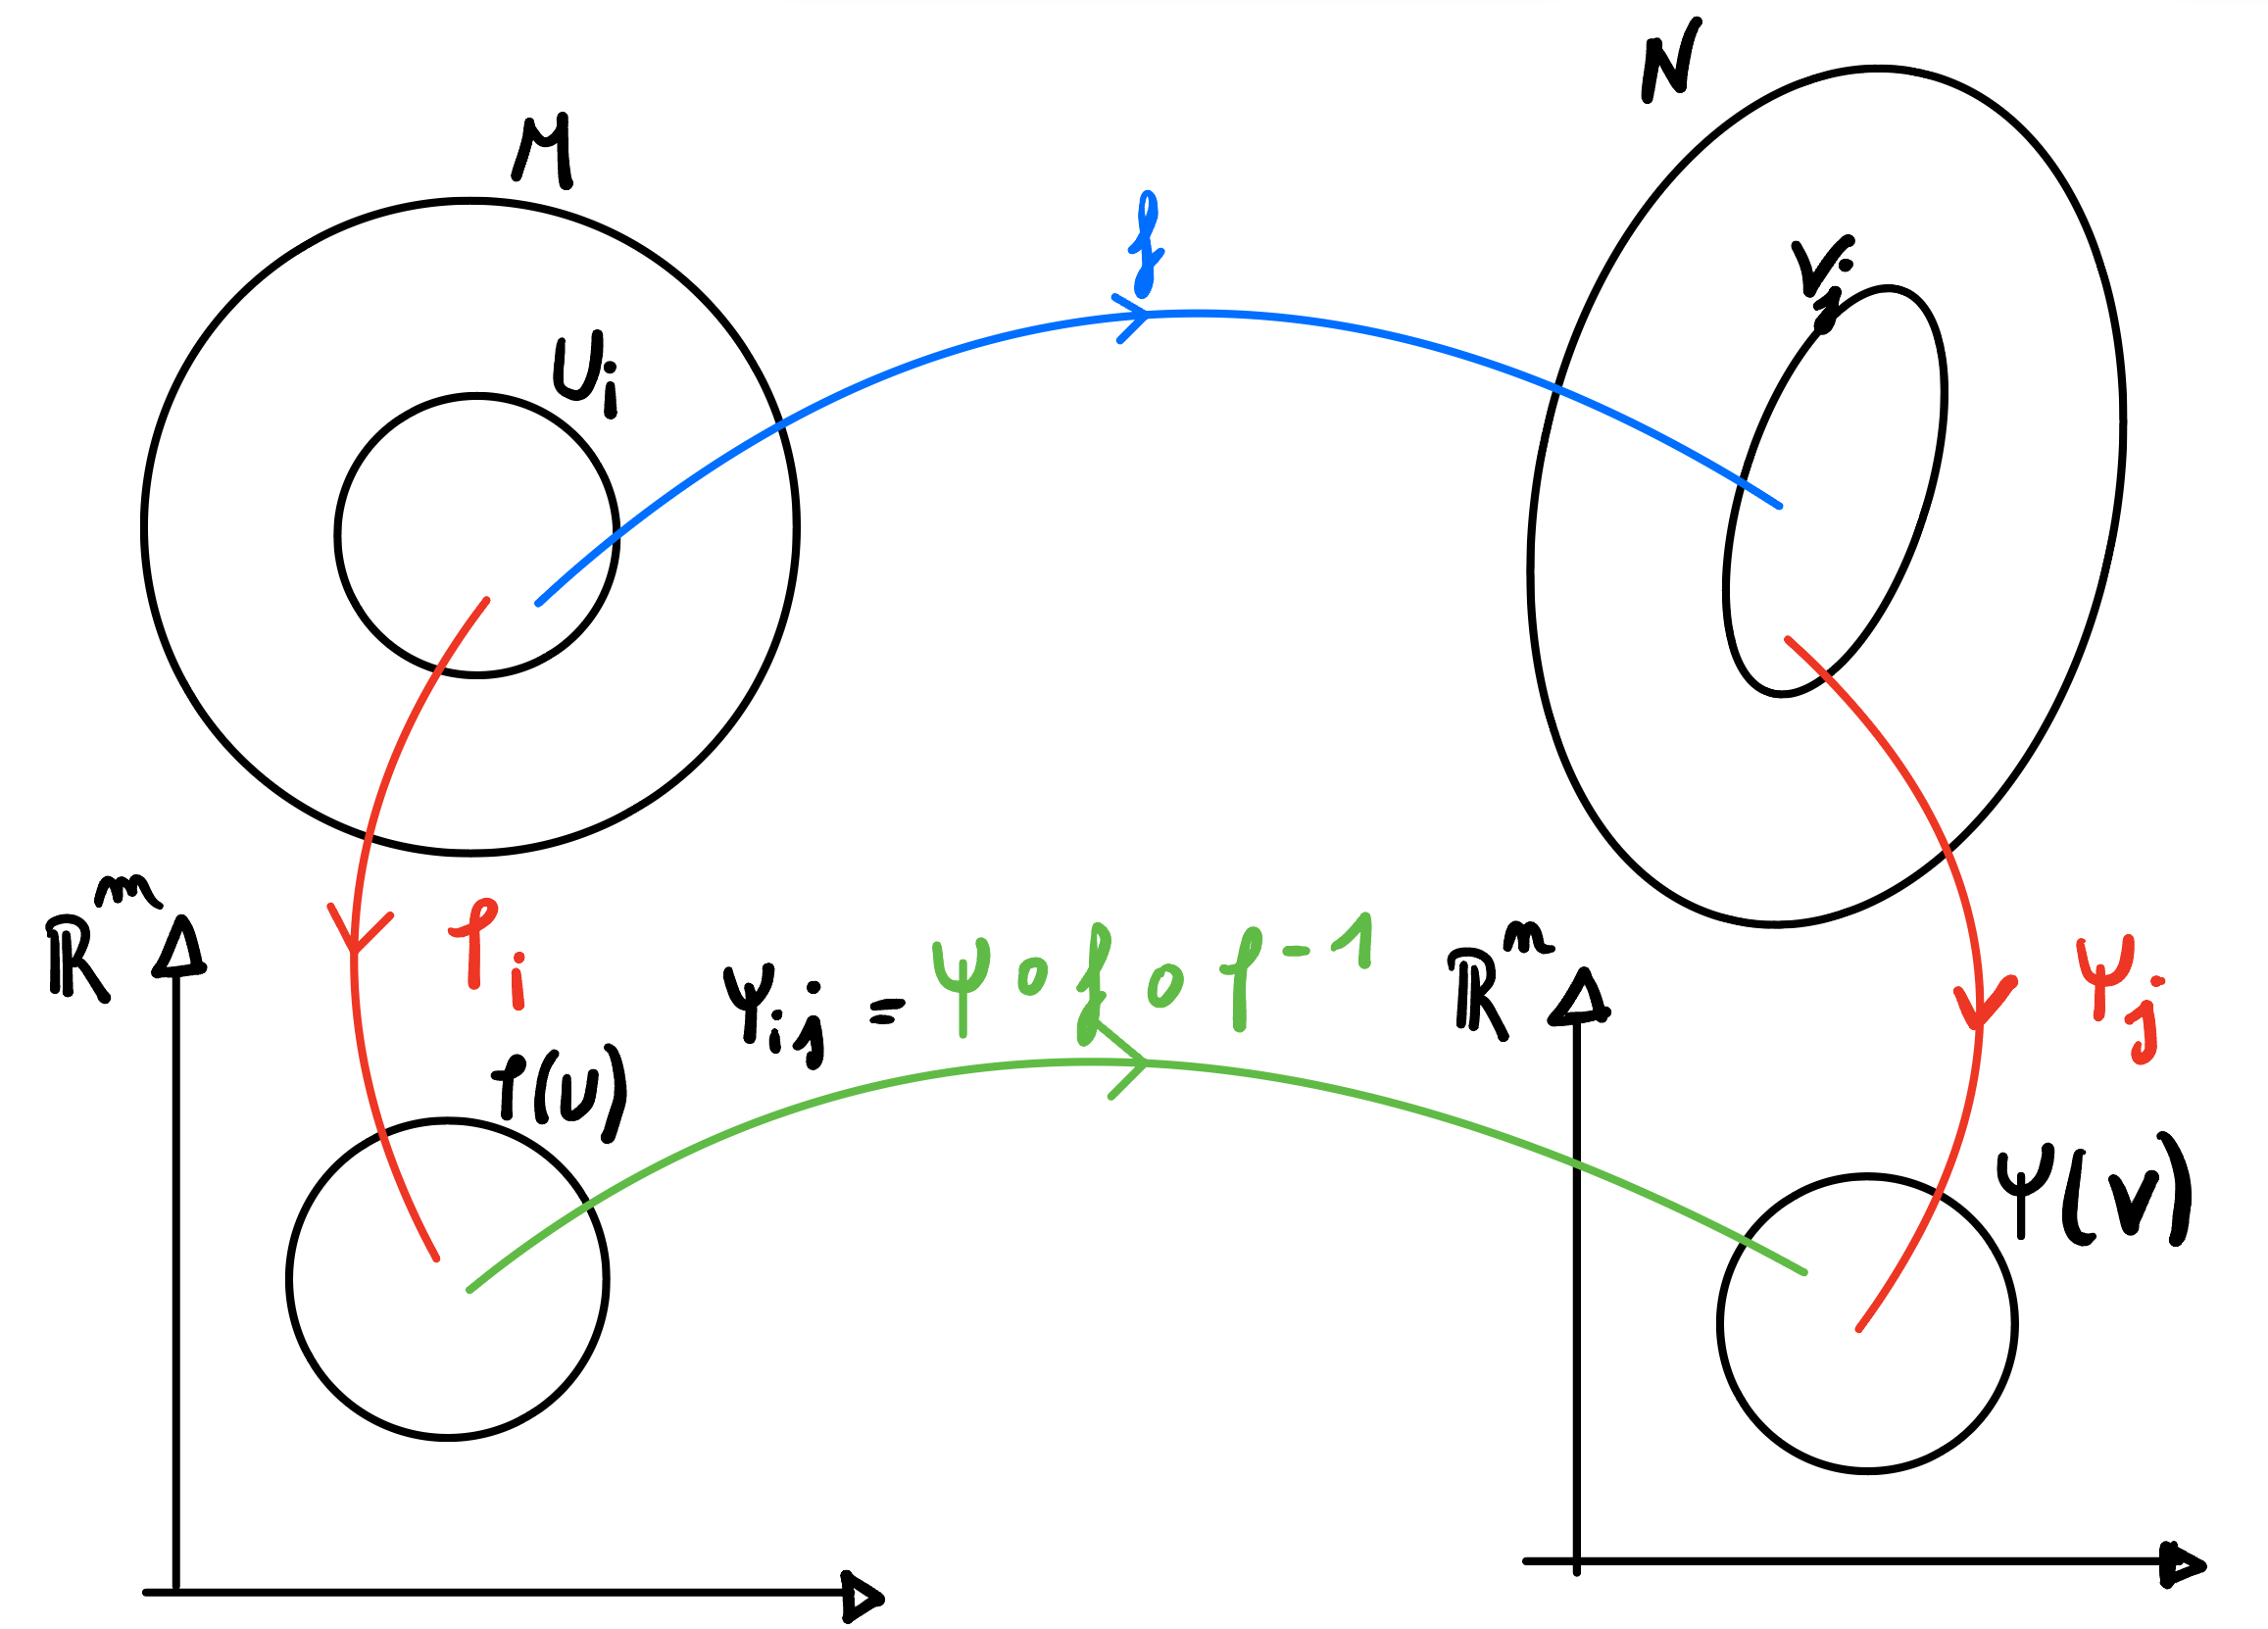
\includegraphics[scale=0.1]{Chapitres/3.Element de géométrie différentielle/Images/fonction de transistion.jpg}
%\captionof{figure}{}
%\label{Parabolique 2}
\end{center}

\subsection{Définition différomorphisme:}

Soient $\mathcal{M}$ et $\mathcal{N}$ deux variétés différentielle. 

\begin{theoremframe}
    \begin{defi}
        Une application $f:\mathcal{M} \to \mathcal{N}$ est un \emph{difféomorphisme} si et seulement si $f$ est bijective et si $f$ et $f^{-1}$ sont lisses. 
    \end{defi}
\end{theoremframe}
Alternativement, $f$ est un difféomorphisme si et seulement si il existe une application lisse $g: \mathcal{N} \to \mathcal{M}$ telle que 
\begin{equation}
    f \circ g = \mathrm{Id}_\mathcal{N} \quad \text{et} \quad g \circ f = \mathrm{Id}_\mathcal{M}
\end{equation}
Lorsqu'il existe un difféomorphisme entre $\mathcal{M}$ et $\mathcal{N}$, on dit qu'ils sont difféomorphes. Deux variétés qui sont difféomorphes sont également dites équivalent. On peut les déformer l'un dans l'autre de manière lisse. Un difféomorphisme va, contrairement à l'homéomorphisme non-lisse, préserver la structure différentielle et non-seulement la structure topologique de la variété. Ainsi, un cube est homéomorphe mais pas difféomorphe à la sphère, car on ne pourra pas se débarrasser des "coins" de manière lisse.

Un exemple de difféomorphisme est le cas du cercle et de l'ellipse. 
L'équation d'un cercle est $x^2 + y^{2 } = 1$ et l'équation d'une ellipse est $(\frac{x}{a})^2 +(\frac{y}{b})^2 = 1 $. On peut passer de l'un a l'autre via le changement de variable $(x, y) \to (\frac{x}{a}, \frac{y}{b})$, qui est linéaire et donc lisse. 

L'ensemble des difféomorphisme d'une variété sur elle-même $f: \mathcal{M} \to \mathcal{M}$ représente l'ensemble des choix et changements de coordonnées pour décrire cette variété. La transformation au niveau des coordonnées est de la forme $x^{\mu}(P)v \to x'^{\mu}(x^{\alpha(\lambda)})$ $\forall P \in \mathcal{M}$. 

\subsection{Interprétation physique des changements de coordonnées:}

Les difféomorphismes (et donc les changements de coordonnées) sur $\mathcal{M}$ peuvent être vus de 2 manières différentes:

\begin{enumerate}
    \item Soit une carte locale $(U,\varphi)$ incluant un point $P$ et notons $\varphi(P) = x^\mu(P) \in \R^m$ (on dit que $x^\mu$ sont les \emph{coordonnées} de $P$ de la carte locale). Un difféomorphisme $f:\mathcal{M} \to \mathcal{M}$ envoie $P$ sur $f(P)$, et on notera $\varphi(f(P)) \equiv y^\mu(P) = x^\mu(f(P))$. C'est ce qu'on appelle une \emph{transformation active des coordonnées}, car le point $P$ change explicitement.

    \begin{center}
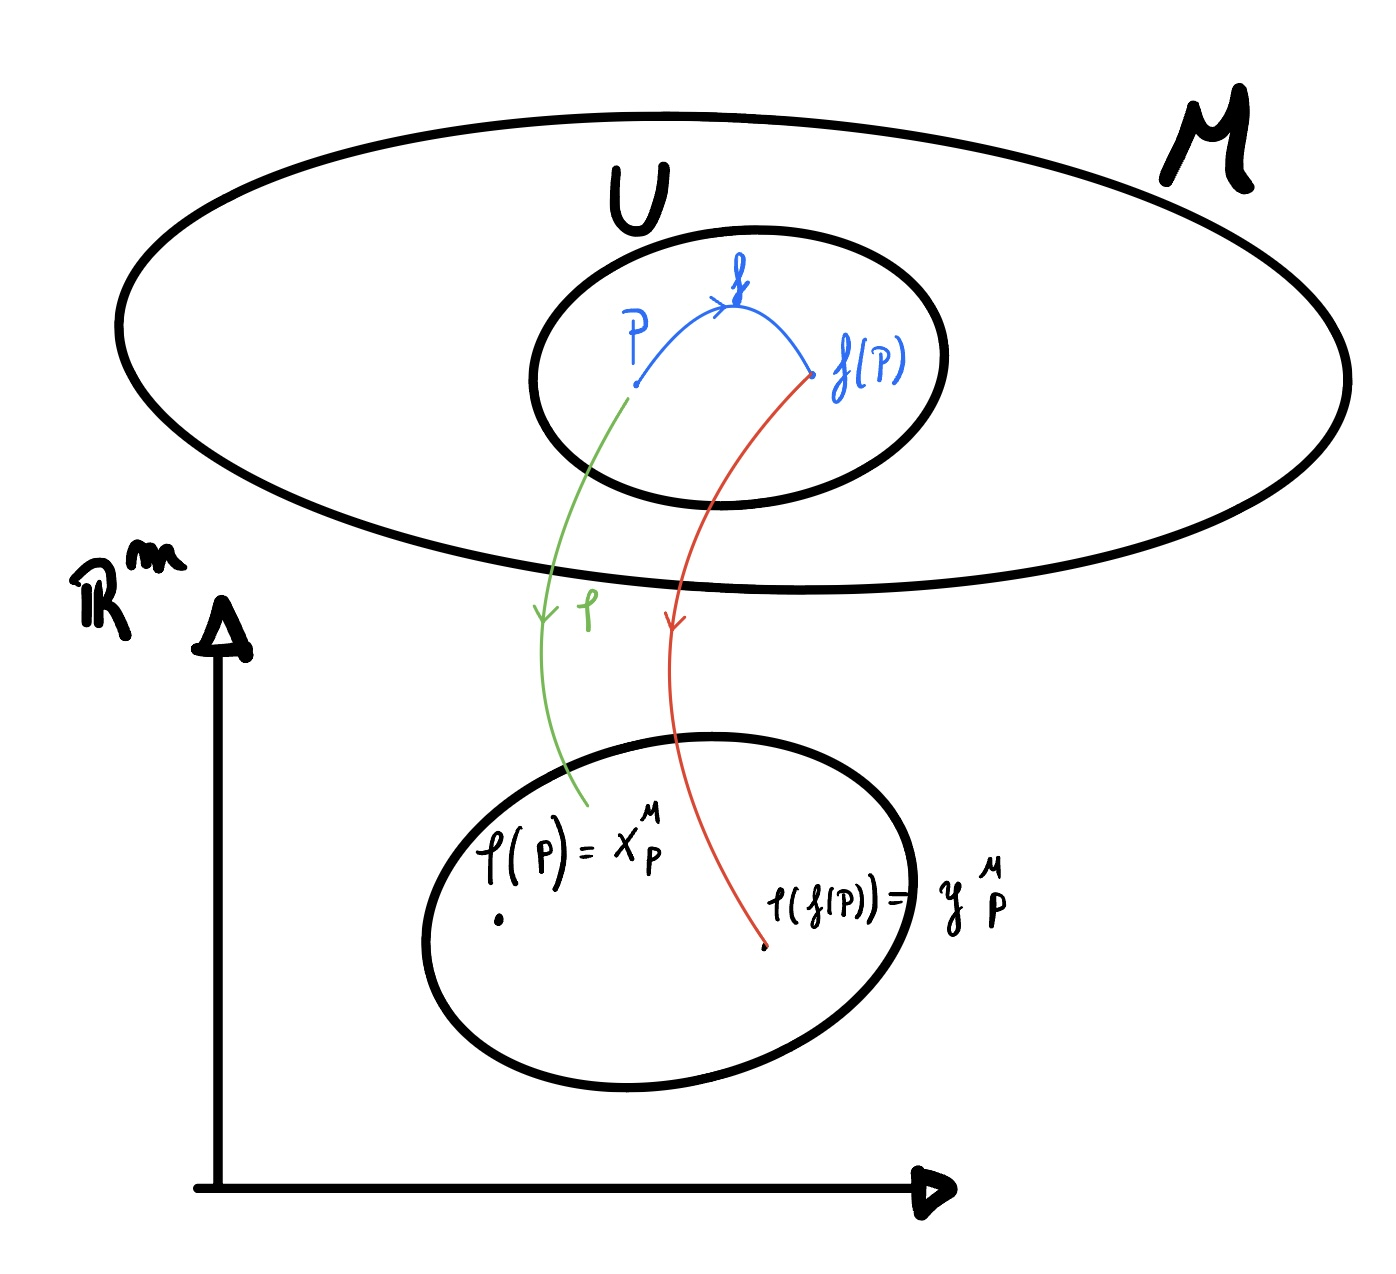
\includegraphics[scale=0.15]{Chapitres/3.Element de géométrie différentielle/Images/transformation actives.jpg}
%\captionof{figure}{}
%\label{Parabolique 2}
\end{center}
\item Soient deux cartes locales de $P$, notées $(U,\varphi)$ et $(V,\psi)$ et notons $\varphi(P) = x^\mu(P)$ et $\psi(P) = y^\mu(P)$. Remarquons que ces deux coordonnées ne coïncident pas nécessairement. Ils sont, liés par la fonction de transition $f = \varphi \circ \psi^{-1}, \, y^\mu \mapsto x^\mu$, qui est un difféomorphisme. Cette représentation est nommée \emph{transformation passive des coordonnées}, car le point $P$ reste le même : la différence vient des deux cartes distinctes utilisées.
\end{enumerate}

\subsection{Un atlas pour $S^2$}
Nous nous chargerons d'illustrer un cas où une carte globale n'existe pas\footnote{Il est un exercice intéressant de montrer qu'une paramétrisation globale n'existe pas. Une intuition peut être donné par le théorème de la boule chevelue.}. Le cas le plus simple est la 2-sphère définie par 
\begin{equation}
    S^2 \equiv \{ (x,y,z) \in \R^3 \mid x^2+y^2+z^2 = 1\}
\end{equation}
Nous allons construire un atlas de $S^2$. Pour ce, nous allons utiliser la \emph{projection stéréographique} : Soit le pôle nord $N = (0,0,1)$. Remarquons que pour tout point $P\in S^2\backslash \{N\}$, il existe une unique droite passant par $P$ et $N$. La projection stéréographique $\varphi_N:S^2\backslash\{N\} \to \R^2$ de $P$ par rapport à $N$ est alors définie comme l'intersection de cette droite avec le plan $z=0$. Selon cette définition, le pôle sud $S = (0,0,-1)$ est envoyé sur $(0,0)$, et lorsque $P \to N$, $\lVert \varphi(P) \lVert \to \infty$.

\begin{figure}[H]
    \centering
    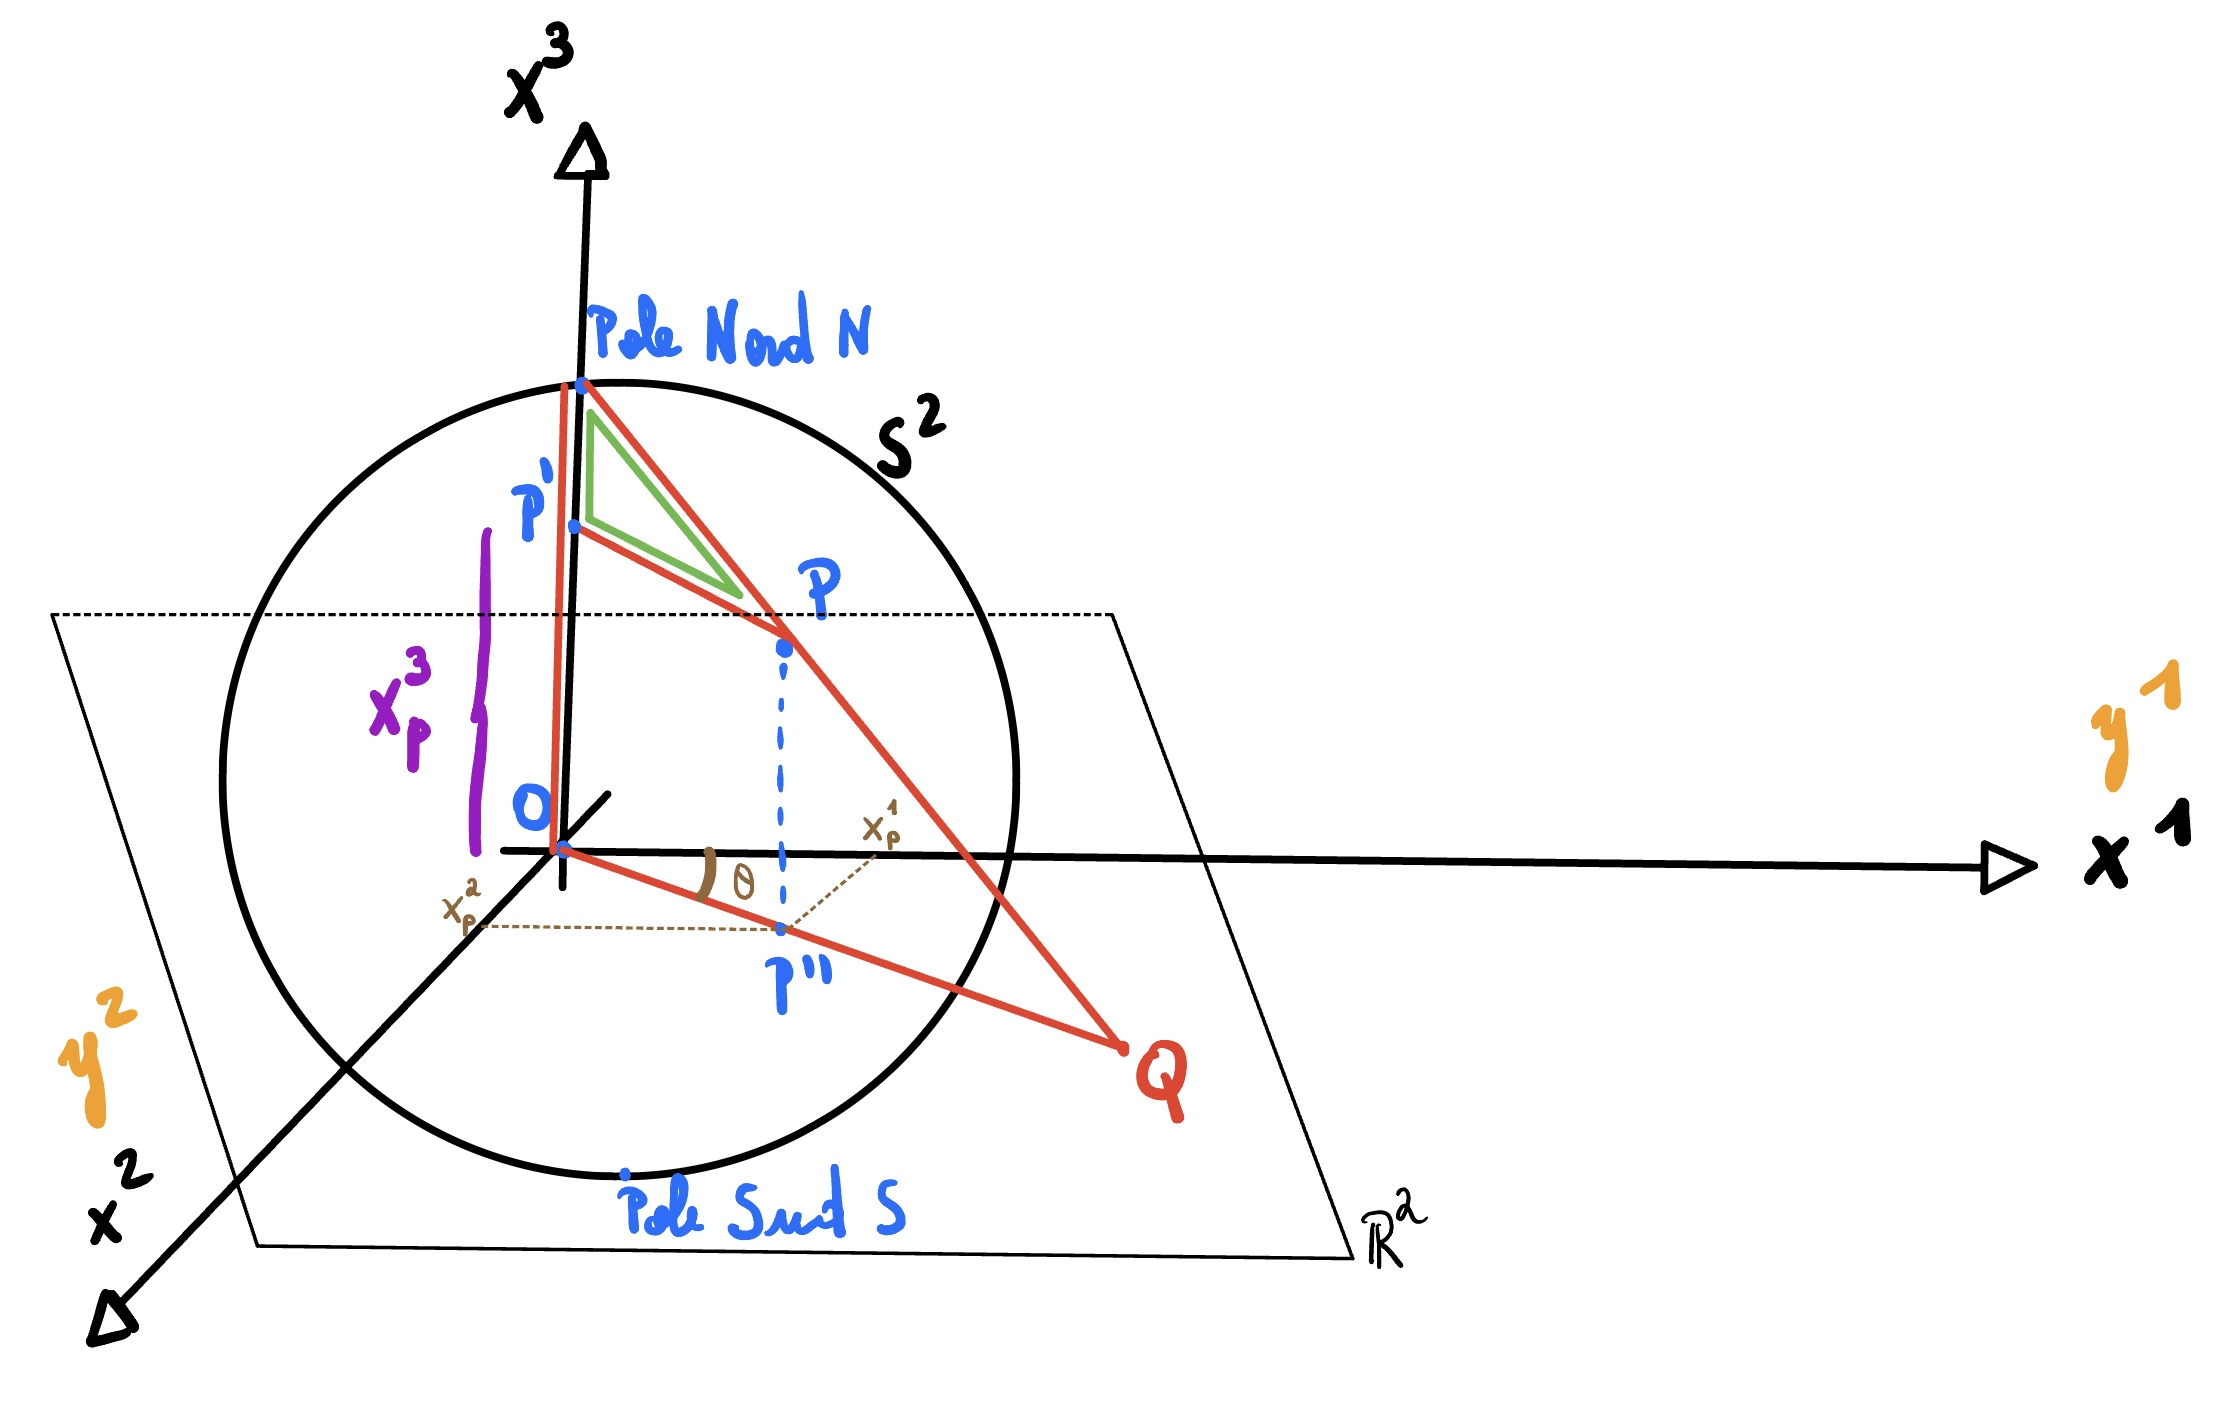
\includegraphics[width=0.7\linewidth]{Chapitres/3.Element de géométrie différentielle/Images/sphère S^2.jpg}
    \caption{Visualisation de la projection stéréographique par rapport à $N$.}
    \label{fig:stereographique 1}
\end{figure}

Dérivons la forme explicite pour $\varphi_N$. Notons $O = (0,0,0)$ et considérons un point $P\in S^2$ ainsi que sa projection stéréographique $Q \in R^2 \times \{0\}$. Notons de plus $P_z$ la projection de $P$ sur l'axe $\vect{u}_z$ et $P_{xy}$ la projection de $P$ sur le plan $Oxy$. Remarquons que les triangles $PP_zN$ et $QON$ sont semblables et donc
\begin{align}
    \frac{OQ}{ON} = \frac{P_zP}{NP_z} \implies OQ = \frac{OP_{xy}}{1-x^3_P}
\end{align}
car $ON = 1$, $P_zP = OP_{xy}$ et $NP_z = 1 - x^3_P$. Finalement, on trouve donc que 
\begin{equation}
    Q^i = \varphi_N(P)^i = \frac{x^i_P}{1-x^3_P}
\end{equation}
où $i=1,2$. La 
\begin{equation}
\label{eq:stereoN}
    \varphi_N : S^2\backslash\{N\} \to \R^2 : (x^1,x^2,x^3) \mapsto \frac{1}{1-x^3} (x^1,x^2)
\end{equation}
Similairement, la projection stéréographique par rapport au pôle sud est
\begin{equation}
    \label{eq:stereoS}
    \varphi_S:S^2\backslash \{S\} \to \R^2 : (y^1,y^2,y^3) \mapsto \frac{1}{1+y^3} (y^1,y^2)
\end{equation}
Montrons à présent que $\{ (S^2\backslash\{N\}, \varphi_N), (S^2\backslash\{S\}, \varphi_S)\}$ est un atlas lisse de $S^2$. Pour ce, nous devons montrer que les fonctions de transitions sont lisses. Posons $\varphi_N^i = z^i$. On a alors
\begin{equation}
\label{eq:1 altasS2}
    z^i = \frac{x^i}{1-x^3}
\end{equation}
Et en utilisant la définition de $S^2$ :
\begin{equation}
    (z^1)^2 + (z^2)^2 = \frac{1 - (x^3)^2}{(1-x^3)^2} = \frac{1 + x^3}{1-x^3}
\end{equation}
Ceci nous permet d'isoler et de réinjecter $x^3$ dans (\ref{eq:1 altasS2}). On trouve alors
\begin{equation}
    \psi_N = \varphi_N^{-1}: \R^2 \to S^2\backslash \{N\}:(u,v) \mapsto \frac{1}{1+u^2 +v^2} \lt 2 u,2v, -1 + u^2+v^2 \rt
\end{equation}
La fonction de transition est alors
\begin{align}
    \varphi_S \circ \psi_N : \psi^{-1}_N \circ \varphi^{-1}_S(\R^2) = \R^2_0 \to \R^2 : (u,v) \mapsto \frac{(u,v)}{u^2+v^2}
\end{align}
Qui est lisse sur $\R^2_0$. Remarquons que $\psi_N(0,0) = (0,0,-1)=S$, donc notre domaine de définition est bien correct (comme $\varphi_S$ n'est pas définie en $S$, nous devons exclure $(0,0)$ du domaine).
\begin{exerc}
    Dérivez l'expression (\ref{eq:stereoS}) pour $\varphi_S : S^2\backslash \{ S\} \to \R^2$. Calculez $\psi_S$ et montrez que $\varphi_N \circ \varphi_S^{-1}$ est bien lisse sur son domaine. 
\end{exerc}
Nous avons trouvé un atlas lisse de $S^2$.
\section{Vecteurs dans une variété}
Nous devons retravailler la notion de vecteur introduite à la section 1.1, afin qu'elle soit intrinsèque à $\mathcal{M}$. Le problème principal est qu'une variété arbitraire n'est pas un espace vectoriel, seulement le plan tangent en est un. Fixons un point $m\in \mathcal{M}$ ($\dim \mathcal{M} = n$) et une courbe $\gamma$ dans $\mathcal{M}$ telle que $\gamma(0)=m$.
\begin{theoremframe}
    \begin{defi}
        Un \emph{vecteur tangent} $X_m$ à $\mathcal{M}$ en $m$ est un opérateur différentiel linéaire agissant sur les fonctions lisses dans un voisinage de $m$ tel que
        \begin{equation}
        \label{eq: vectvar}
            X_m f =\left. \frac{\td}{\td \lambda}\right|_{\lambda=0}  f \circ \gamma(\lambda)
        \end{equation}
    \end{defi}
\end{theoremframe}
Un vecteur tangent peut donc être vu comme une dérivée directionnelle s'appliquant sur les fonctions le long d'une courbe en $\lambda=0$. Nous abuserons parfois de cette notation en écrivant $X = \frac{\td}{\td \lambda}$. Notons que (\ref{eq: vectvar}) s'écrit en composantes :
\begin{equation}
    X_i f = \left. \frac{\td}{\td \lambda}\right|_{\lambda=0}  f \circ \gamma_i(\lambda).
\end{equation}
Soit une carte locale $(U,\varphi)$ de $\mathcal{M}$ au point $m$. Notons $F = f \circ \varphi^{-1} : \R^m\to \R$ et $x^\mu(\gamma) = \varphi \circ \gamma: \R \to \R^m$ les représentations en coordonnées de $f$ et $\gamma$ dans cette carte locale. On trouve alors
\begin{align}
    X_m f = \left. \frac{\td}{\td \lambda}\right|_{\lambda=0}  f \circ \gamma(\lambda) &= \left. \frac{\td}{\td \lambda}\right|_{\lambda=0}  f \circ \varphi^{-1} \circ \varphi \circ \gamma(\lambda)\\
    & = \left. \frac{\td}{\td \lambda}\right|_{\lambda=0}  F \circ x^\mu(\gamma((\lambda))
\end{align}
S'agissant à présent de fonctions dans des espaces euclidiens, nous pouvons appliquer la règle de la chaine.
\begin{align}
    X_mf = \left. \frac{\pd F}{\pd x^\mu} \right|_{x^\mu=x^\mu(m)} \left. \frac{\pd x^\mu}{\pd \lambda} \right|_{\lambda = 0} (\gamma(\lambda))
\end{align}
En omettant la différence entre la fonction $f$ et sa représentation locale $F$, nous écrirons
\begin{align}
    X_m f = \left. \frac{\td}{\td \lambda} \right|_{\lambda=0} f = \left. \frac{\td x^\mu}{\td \lambda} \right|_{\lambda = 0} \frac{\pd}{\pd x^\mu}f
\end{align}
Comme $f$ est arbitraire, nous trouvons
\begin{equation}
    X_m = \left. \frac{\td x^\mu}{\td \lambda} \right|_{\lambda = 0} \frac{\pd}{\pd x^\mu}
\end{equation}
où les premiers termes sont les composantes du vecteur $X_m$ et les deuxièmes termes $\{\pd_\mu \}$ forment une base de l'espace $T_m\mathcal{M}$. Remarquons que donc, la dimension de $T_m\mathcal{M}$ est $n$.
\begin{center}
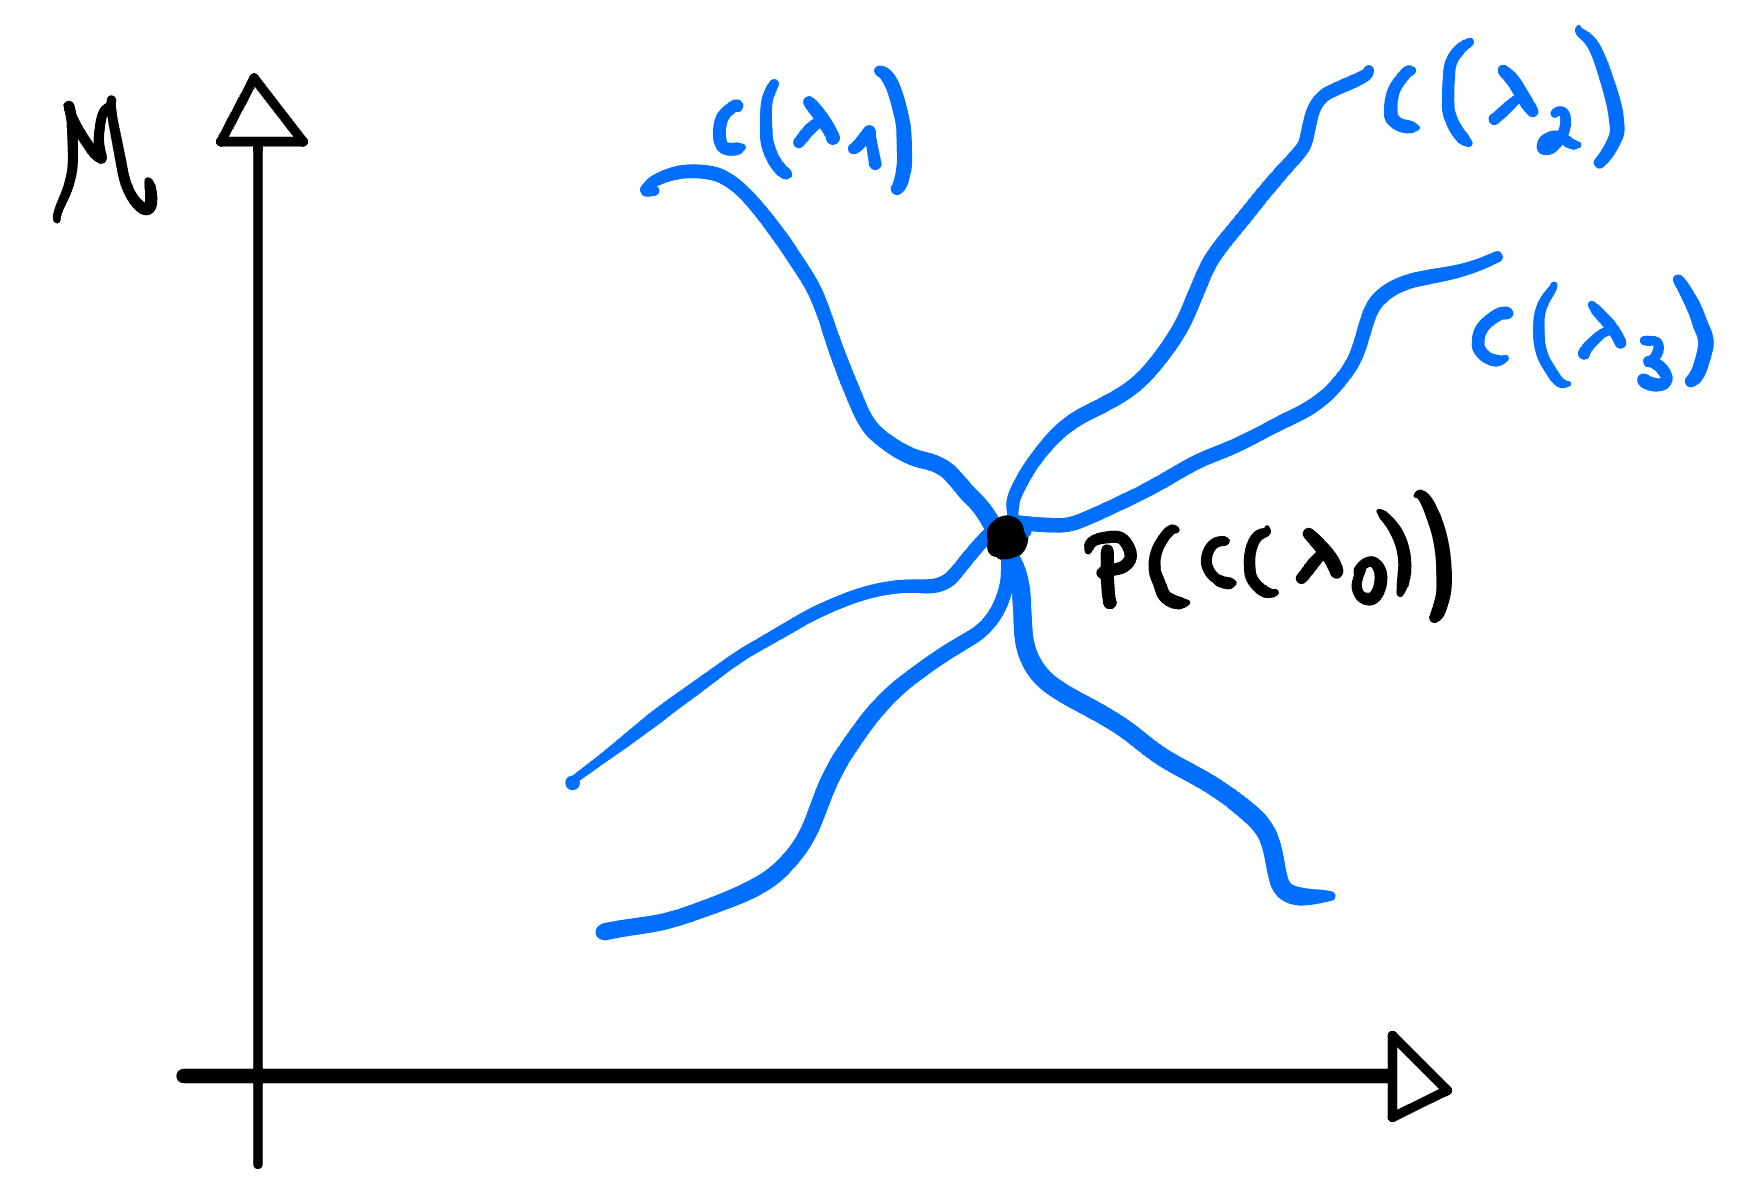
\includegraphics[scale=0.1]{Chapitres/3.Element de géométrie différentielle/Images/vecteurs2.0.jpg}
%\captionof{figure}{}
%\label{Parabolique 2}
\end{center}


\begin{center}
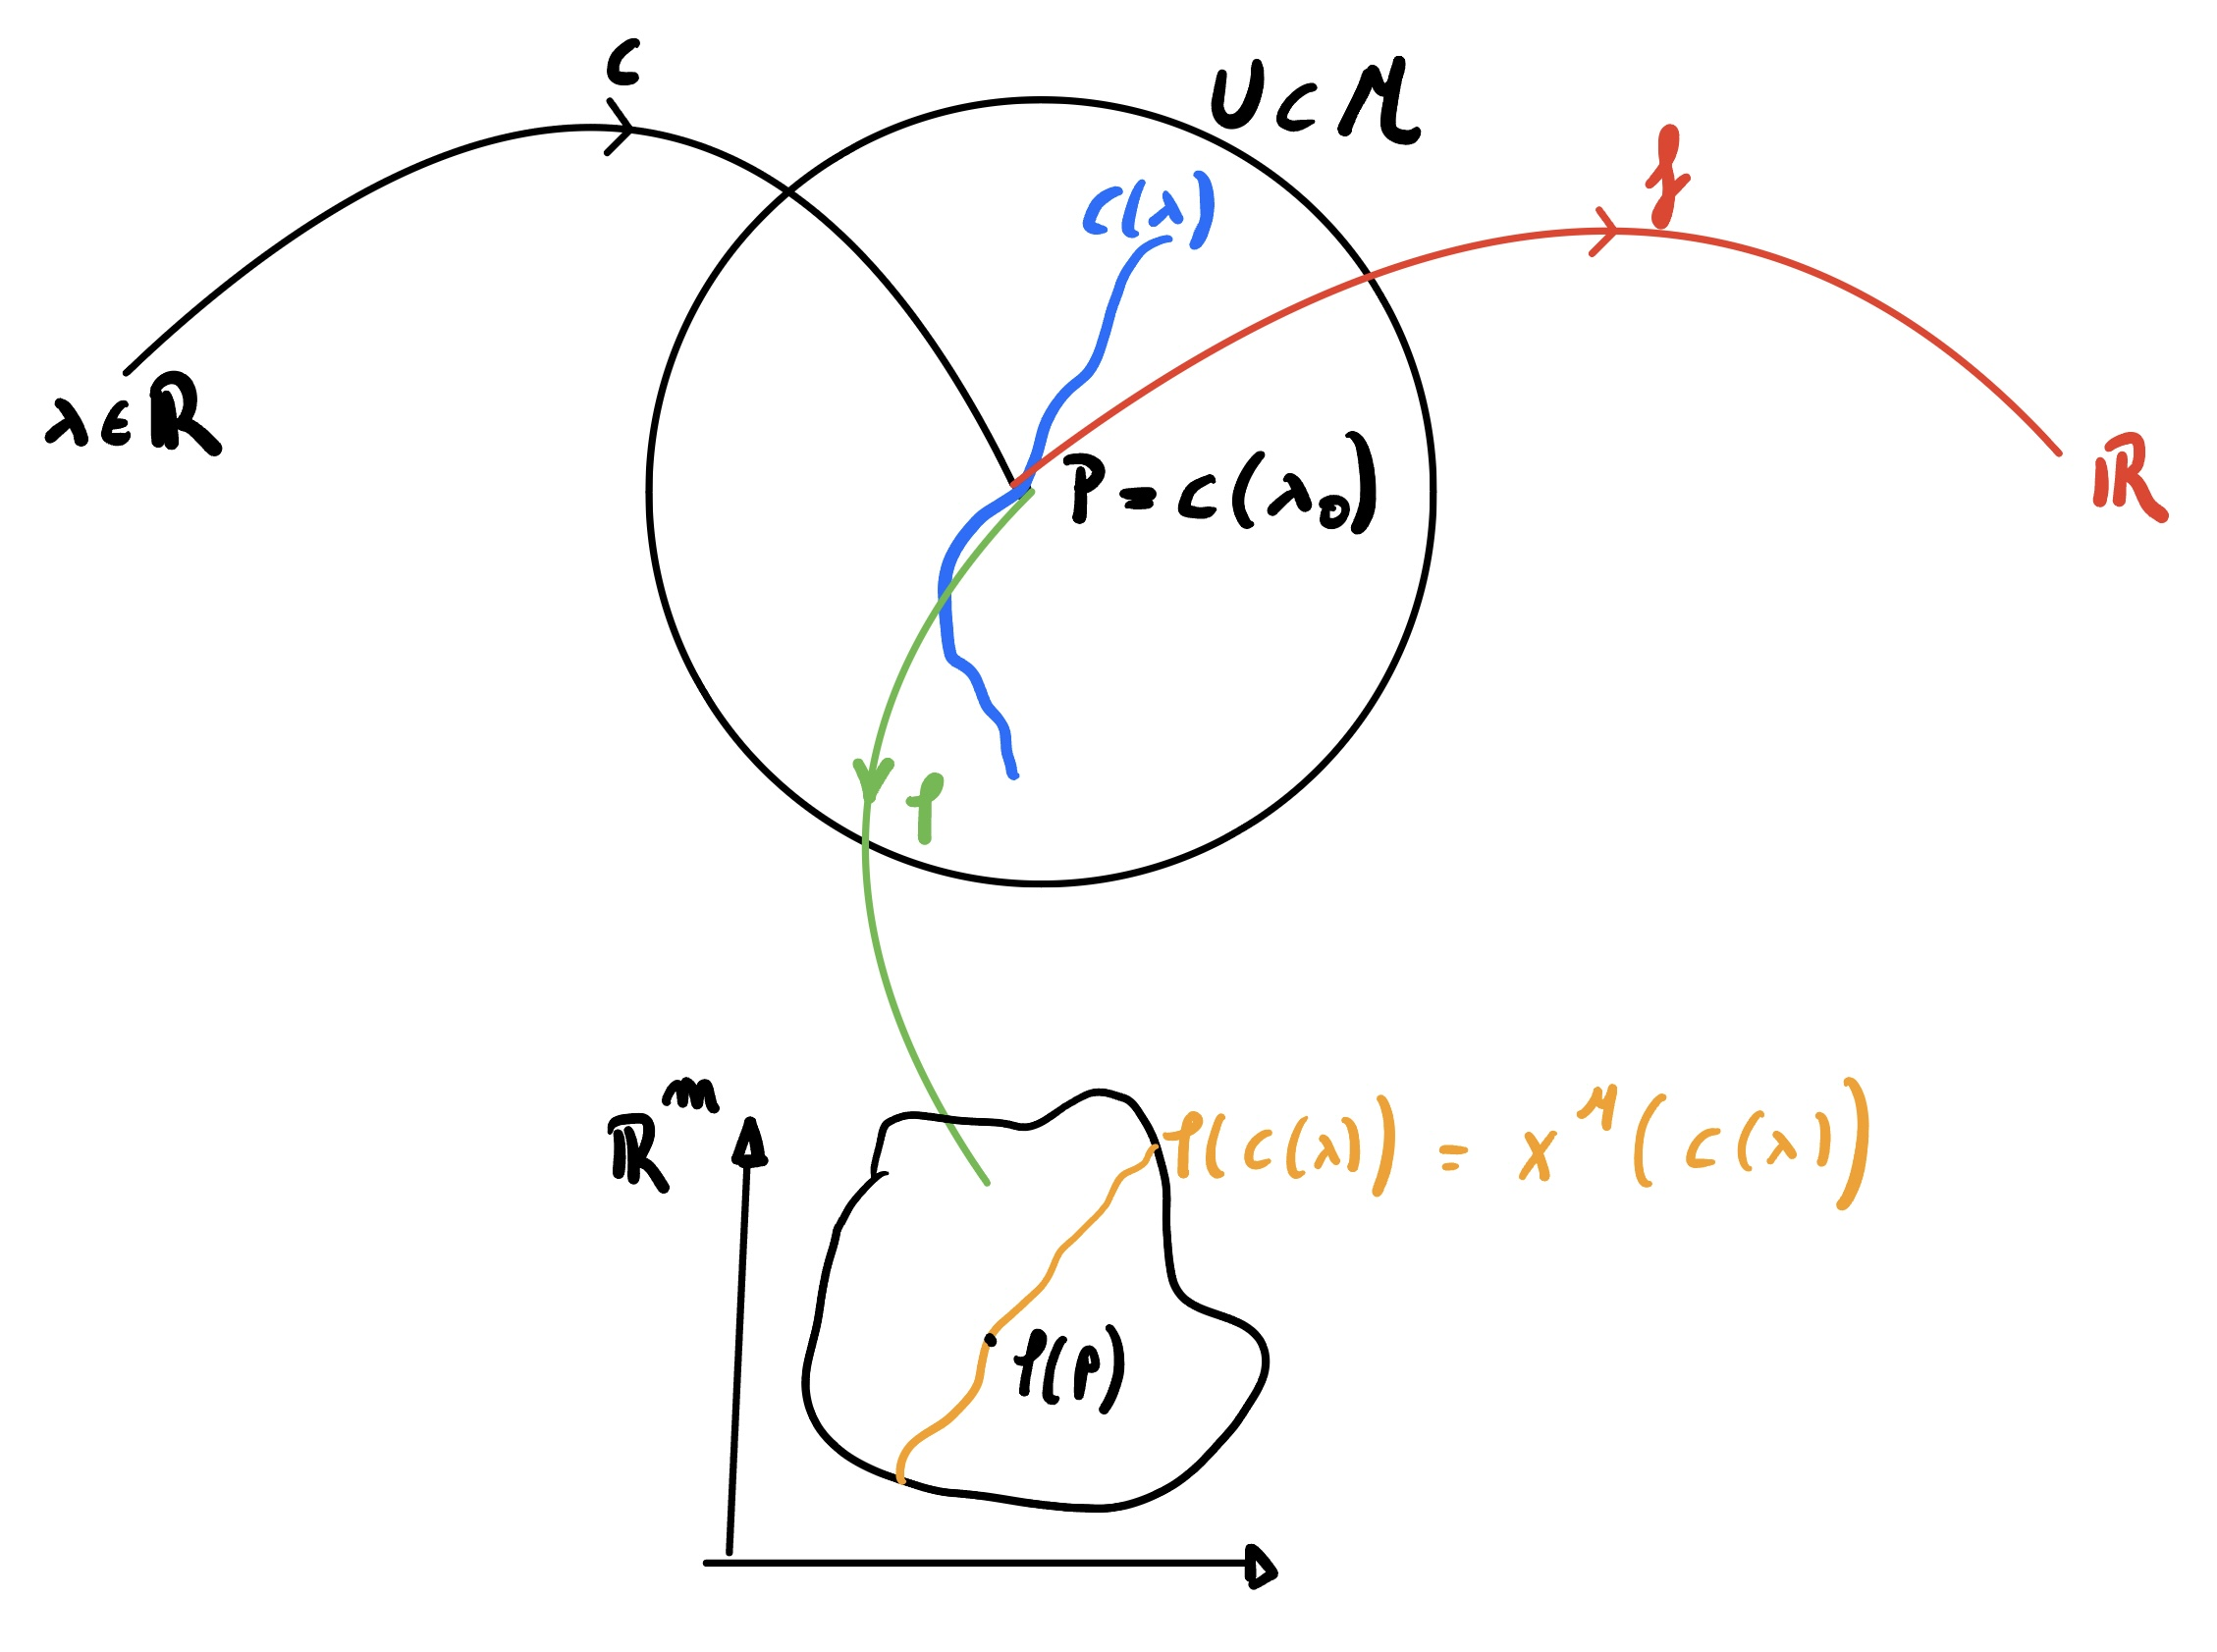
\includegraphics[scale=0.1]{Chapitres/3.Element de géométrie différentielle/Images/dimenson.jpg}
%\captionof{figure}{}
%\label{Parabolique 2}
\end{center}


De manière plus concise, on notera

\begin{equation*}
    X = \frac{\td}{\td \lambda }= \frac{\td x^{\mu}}{\td \lambda } \frac{\partial }{\partial x^{\mu}} = X^{\mu} \partial_{\mu}
\end{equation*}

où nous sous-entendons $x^{\mu} = x^{\mu}( \gamma(\lambda))$. Les vecteurs $X = \pd_\mu$ représentent un déplacement tangent à la direction $x^\mu$. Contrairement à la variété $\mathcal{M}$, qui n'est pas un espace vectoriel dans le cas général, l'espace tangent en est un. 
\begin{center}
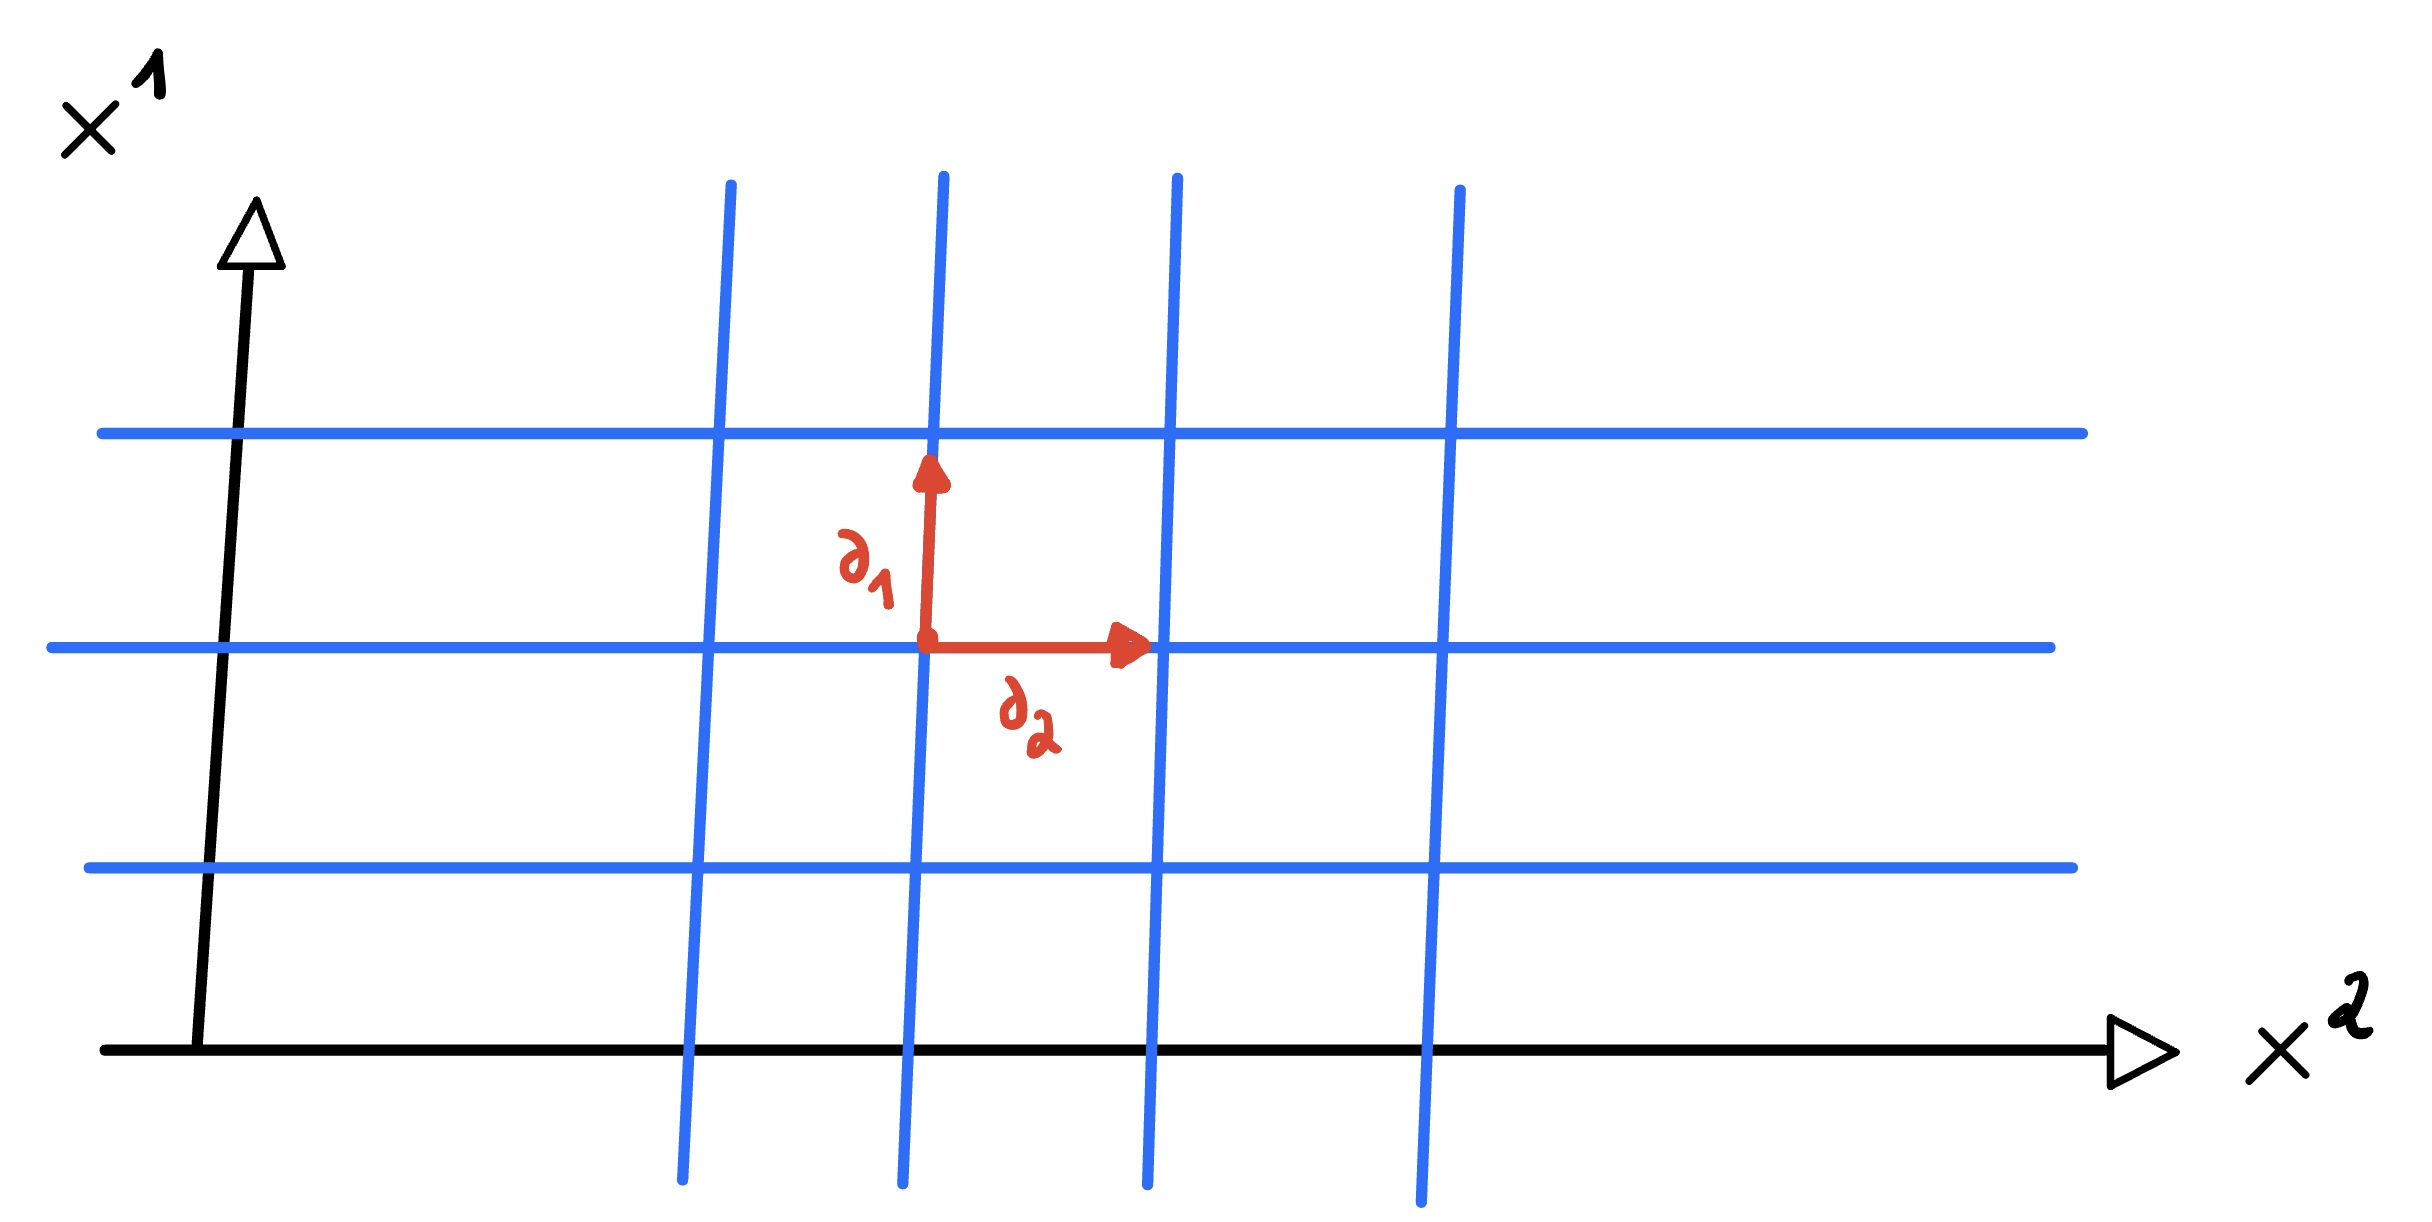
\includegraphics[scale=0.1]{Chapitres/3.Element de géométrie différentielle/Images/vecteur-fleche.jpg}
%\captionof{figure}{}
%\label{Parabolique 2}
\end{center}
\subsubsection{Loi de transformation des vecteurs}
Les vecteurs sont indépendants de la base et du choix de la carte locale. Sous changement général de coordonnées (difféomorphisme), les composantes $X_\mu$ d'un vecteur se transforment selon
    \begin{align}
        \boxed{X^\mu \to X^{\mu'} = \frac{\td x^{\mu'}}{\td \lambda} = \frac{\pd x^{\mu'}}{\pd x^\alpha} \frac{\td x^\alpha}{\td \lambda} = \frac{\pd x^{\mu'}}{\pd x^\alpha} X^\alpha}
    \end{align}
Similairement, les vecteurs de base se transforment selon
\begin{equation}
    \pd_\alpha \to \pd_{\alpha'} = \frac{\pd x^\mu}{\pd x^{\alpha'}} \pd_\mu
\end{equation}
de sorte que $X$ soit invariant sous difféomorphisme. Remarquons qu'il s'agit ici simplememnt de la règle de la chaîne. Notons les identités suivantes de la jacobienne $\frac{\pd x^{\mu'}}{\pd x^\alpha}$.
\begin{align}
    \label{eq: id chgmt de coordonnées}
    \boxed{
        \begin{array}{c}
            \displaystyle
            \dfrac{\pd x^{\mu'}}{\pd x^\alpha}\dfrac{\pd x^{\beta}}{\pd x^{\mu'}} = \displaystyle \delta^\beta_\alpha  \\
            \\
            \dfrac{\pd x^{\alpha}}{\pd x^{\nu'}}\dfrac{\pd x^{\mu'}}{\pd x^\alpha} =\displaystyle\delta\indices*{^{\mu'}_{\nu'}}
        \end{array} 
    }
\end{align}
\begin{exerc}
    Démontrez ces égalités.
\end{exerc}
Pour récapituler, nous avons trouvé qu'un vecteur dans $T_m\mathcal{M}$ peut être vu comme une application
\begin{equation}
    X_m:C^\infty(U) \to \R:f \mapsto X_m f = \left. X^\mu_m \pd_\mu f \right|_{x^\mu(m)}
\end{equation}
où $U$ est un voisinage de $m$. Nous définirons par ailleurs un champ de vecteurs comme la donnée d'un vecteur en tout point $m \in \mathcal{M}$.
\begin{equation}
    \chi: T\mathcal{M} \to \R
\end{equation}
Où $T\mathcal{M}$ est le fibré tangent. Le champ de vecteurs est dit lisse s'il dépend lissement du point $m$ (dans le sens des représentations locales de coordonnées). L'ensemble des champs de vecteurs lisses sur $\mathcal{M}$ est noté $ \Zhe (\mathcal{M})$.

\subsection{Covecteurs}

Soit $X_m \in T_m \mathcal{M}$. Un covecteur $w\in T_m^*\mathcal{M}$ est une forme linéaire sur $T_m\mathcal{M}$ 
\begin{equation}
w  : T_m \mathcal{M} \rightarrow \R : X \mapsto w(X)
\end{equation}
où pour rappel l'espace $T^*_m \mathcal{M}$ est le dual de $T_m\mathcal{M}$, également appelé l'espace cotangent. 

\begin{exmp}
    Soit $f\in C^\infty(\mathcal{M})$. La différentielle $\td f$ de $f$ au point $m\in \mathcal{M}$ est un covecteur. Son action est définie par
    \begin{equation}
        \left. \td f \right|_m : T_m \mathcal{M} \to \R : \td f (X) = X(f) = \left. X^\mu_m \pd_\mu f \right|_m.
    \end{equation}
On se souviendra qu'une base de l'espace cotangent est donnée par $\{ \td x^\nu\}$. Nous avions également trouvé que la relation entre la base de l'espace tangent et de l'espace cotangent est
\begin{equation}
    \td  x^\mu (\pd_\nu) = \delta\indices*{^\mu_\nu}
\end{equation}
Suivant notre définition de covecteur, nous pouvons à présent justifier cette relation. En effet, soit $X = \pd_\nu$. Alors
\begin{equation}
    \td x^\mu \lt \frac{\pd}{\pd x^\nu}\rt \equiv \frac{\pd}{\pd x^\nu}(x^\mu) = \delta\indices*{^\mu_\nu}
\end{equation}
Dans une carte locale, nous décomposer $\td f$ sur la base selon
\begin{equation}
    \td f = \frac{\pd f}{\pd x^\mu} \td x^\mu
\end{equation}
\end{exmp}
Montrons à présent que selon notre définition, $w(X)$ est bien scalaire. Dans une carte locale, on a
\begin{equation}
    w(X) = w_\mu \td x^\mu (X^\nu \pd_\nu ) = w_\mu X^\nu \td x^\mu (\pd_\nu) = w_\mu X^\nu \delta\indices*{^\mu_\nu} = w_\mu X^\mu
\end{equation}
Où nous avons utilisé la linéarité de $\td x^\mu$. On conclut que $w(X)$ est bien un scalaire. Sous changements de coordonnées général (difféomorphisme), on trouve donc via l'invariance de $w(X)$ et la loi de transformation de $X$ que
\begin{equation}
    w_\mu X^\mu = w_{\mu'} X^{\mu'} = w_{\mu'} \frac{\pd x^{\mu'}}{\pd x^\mu} X^\mu
\end{equation}
Où on peut donc identifier
\begin{equation}
    w_\alpha = w_{\alpha'} \frac{\pd x^{\alpha'}}{\pd x^\alpha}
\end{equation}
En inversant cette relation via (\ref{eq: id chgmt de coordonnées}), on obtient finalement la loi de transformation sous changement de coordonnées général pour un covecteur

 \begin{equation}
     \boxed{w_\mu \to w_{\mu '} = \frac{\partial x^{\alpha }}{\partial x^{\mu '}} w_{\alpha}}
 \end{equation}

Les vecteurs de bases se transforment comme

$$dx^{\mu'} = \frac{\partial x^{\mu'}}{\partial x^{\alpha}} dx^{\alpha}$$
\subsection{Les tenseurs généraux}
Comme nous nous intéresserons exclusivement à des espaces à dimension finie, $(T^*_m \mathcal{M})^* \simeq T_m \mathcal{M}$ : les vecteurs peuvent êtres vues comme formes linéaires sur l'espace cotangent.
\begin{equation}
    V: T^*_m \mathcal{M} \to \R : w \mapsto V(w) \equiv w(V )
\end{equation}
Soit un point $m\in \mathcal{M}$
\begin{theoremframe}
    \begin{rap}
        \label{rap:tenseur}
        Un \emph{tenseur} de type $(p,q)$ est une forme multilinéaire 
        \begin{equation}
            \underbrace{T^*_{m}\mathcal{M} \times \cdots \times T^*_{m}\mathcal{M}}_\text{$p$-fois} \times \underbrace{T_{m}\mathcal{M} \times \cdots \times T_{m}\mathcal{M}}_\text{$q$-fois}  \to \mathbb{R}
        \end{equation}
    \end{rap}
\end{theoremframe}
\begin{exmp} Donnons quelques exemples\\
    \begin{enumerate}
        \item Un \emph{vecteur} est un objet 
        \begin{equation}
            X:T_m^*\mathcal{M} \to \R
        \end{equation}
        et est donc un tenseur $(1,0)$. Dans une carte locale, celui-ci s'écrit $X^\mu \pd_\mu$. Remarquons qu'on a bien $X(\omega) \in \R$.
        \item Un \emph{covecteur} est un objet 
        \begin{equation}
            w:T_m\mathcal{M} \to \R
        \end{equation}
        et est donc un tenseur $(0,1)$. Dans une carte locale, celui-ci s'écrit $w_\mu \td x^\mu$.
        \item De manière générale, les composantes d'un tenseur quelconque $(p,q)$ possèdent $p$ indices contravariants et $q$ indices covariants. Dans une carte locale, le tenseur s'écrit
        \begin{equation}
            T = T\indices{^{\alpha_1} ^{\cdots}^{\alpha_p}_{\nu_1}_{\cdots} _{\nu_q}} \partial_{\alpha_{1}}
            \otimes ... \otimes \partial_{\alpha_{p}} \otimes dx^{\nu_{1}}\otimes...\otimes dx^{\nu_{q}} 
        \end{equation}
        Ses composantes se transforment sous changement de coordonnées général selon
        \begin{equation}
            T\indices{^{\alpha_1} ^{\cdots}^{\alpha_p}_{\nu_1}_{\cdots} _{\nu_q}} \to T\indices{^{\alpha'_1} ^{\cdots}^{\alpha'_p}_{\nu'_1}_{\cdots} _{\nu'_q}} = \frac{\partial x^{\alpha'_1}}{\partial x^{\alpha_1}} \cdots\frac{\partial x^{\alpha'_p}}{\partial x^{\alpha_p}}\frac{\partial x^{\nu_1}}{\partial x^{\nu'_1}}\cdots\frac{\partial x^{\nu_q}}{\partial x^{\nu'_q}} T\indices{^{\alpha_1} ^{\cdots}^{\alpha_p}_{\nu_1}_{\cdots} _{\nu_q}}
        \end{equation}
    \end{enumerate}
\end{exmp}
\section{Les p-formes différentielles}
Nous souhaitons pouvoir définir une structure différentielle sur notre variété, c'est-à-dire construire une manière de différentier un tenseur quelconque sur notre variété, qui nous permettrait d'étudier des systèmes dynamiques dans notre variété (i.e. des équations différentielles). Or, un problème apparaît lorsqu'on s'intéresse à la quantité $\pd_\mu w_\nu$. Sous changement général de coordonnées, cette quantité varie selon
\begin{align}
\nonumber
    \label{eq: not a tensor}
    \pd_\mu w_\nu \to \pd_{\mu'} w_{\nu'} &= \frac{\pd x^\mu}{\pd x^{\mu'}} \pd_\mu \lt \frac{\pd x^\nu}{\pd x^{\nu'}} w_\nu \rt\\
    & = \frac{\pd x^\mu}{\pd x^{\mu'}} \frac{\pd x^\nu}{\pd x^{\nu'}} \pd_\mu w_\nu + \frac{\pd x^\mu}{\pd x^{\mu'}} w_\nu \frac{\pd}{\pd x^\mu}  \frac{\pd x^\nu}{\pd x^{\nu'}}\\
    \nonumber
    &= \frac{\pd x^\mu}{\pd x^{\mu'}} \frac{\pd x^\nu}{\pd x^{\nu'}} \pd_\mu w_\nu + w_\nu  \frac{\pd^2 x^\nu}{\pd x^{\mu'}\pd x^{\nu'}}
\end{align}
Où nous avons utilisé la règle de la chaîne pour passer de la deuxième à la troisième ligne. Ainsi, comme sous changement de coordonnées général le deuxième terme ne s'annule pas, $\pd_\mu w_\nu$ \emph{n'est pas un tenseur}. La relation (\ref{eq: not a tensor}) motivera la notion de \emph{p-forme différentielle}.
\begin{theoremframe}
    \begin{defi}
        Une $p$-forme différentielle est un tenseur de type $(0,p)$ totalement antisymétrique.
    \end{defi}
\end{theoremframe}
\begin{propri}
    L'ensemble des p-formes en un point $m\in \mathcal{M}$, noté $\Omega\indices*{^p_m}$ forme un espace vectoriel.
\end{propri}

Par exemple, une 2-forme est une application telle que 

\begin{equation}
    F: T_m\mathcal{M}\times T_m\mathcal{M}\rightarrow \R: (X, Y)\mapsto F(X, Y) = -F(Y, X)
\end{equation}

En composantes\footnote{Nous omettrons dans la suite de préciser la validité dans une carte locale.}, cette 2-forme s'écrit

\begin{equation}
    F(\partial_{\alpha}, \partial_{\beta}) = F_{\mu \nu} dx^{\mu}\otimes dx^{\nu}(\partial_{\alpha}, \partial_{\beta}) = F_{\mu \nu} \delta^{\mu}_{\nu}\delta^{\nu}_{\beta } = F_{\alpha \beta}
\end{equation}
où $F_{\alpha \beta}$ sont les composantes du tenseurs $F$. Comme $F$ est antisymétrique alors $F(\partial_{\alpha}, \partial_{\beta}) = -F(\partial_{\beta}, \partial_{\alpha}) = -F_{ \beta \alpha}$. L'antisymétricité en les arguments implique donc l'antisymétricité en les indices des composantes.
\begin{rmk}
    Notons les espaces suivants :
    \begin{enumerate}
        \item Une 1-forme est un covecteur : $\Omega_m^1 = T_m^*\mathcal{M}$
        \item Une 0-forme est une fonction : $\Omega_m^0 = \left. C^\infty(\mathcal{M}) \right|_m$
    \end{enumerate}
\end{rmk}

\subsubsection{Base et dimension de $\Omega_m^p$}

  Introduisons la notion de \emph{wedge-product}, généralisant le produit vectoriel à une dimension quelconque.
\begin{theoremframe}
    \begin{defi}
        Le wedge-product est défini comme l'opération 
        \begin{equation}
        \wedge : T_m\mathcal{M} \times T_m\mathcal{M} \to T_m \mathcal{M} \otimes T_m\mathcal{M}
        \end{equation}
        tel que
        \begin{equation}
            \td x^{\mu_1}\wedge \cdots\wedge \td x^{\mu_r} = \sum_{\sigma \in S_r} \sgn(\sigma) \td x^{\mu_{\sigma(1)}} \otimes \cdots \otimes \td x^{\mu_{\sigma(r)}}
        \end{equation}
    \end{defi}
\end{theoremframe}
où $S_r$ est le groupe des permutations à r-éléments. Ce groupe contient $r!$ éléments. $\sgn(\sigma)$ est le signe de la permutation $\sigma$, c'est à dire $(-1)^k$ où $k$ est le nombre de permutations nécessaire pour retrouver l'identité. Pour en donner, un exemple simple :
\begin{equation*}
    \mathrm{Id_r} = 
    \begin{pmatrix}
        1 & 2 & 3 & \cdots & r \\
        1 & 2 & 3 & \cdots & r 
    \end{pmatrix}
\end{equation*}

En comparant à la permutation suivante :
\begin{equation*}
    s = 
    \begin{pmatrix}
        1 & 2 & 3 & \cdots & r \\
        2 & 1 & 3 & \cdots & r 
    \end{pmatrix}
\end{equation*}

Alors le signe de $s$ vaut $-1$.

Un élément général de $S_r$ s'écrite 
\begin{equation*}
\sigma = \begin{pmatrix}
1 & 2 & 3 & \cdots & r \\
\sigma(1) & \sigma(2) & \sigma(3) & \cdots & \sigma(r) 
\end{pmatrix}
\end{equation*}

\begin{exmp}
    Donnons quelques exemples de \emph{wedge-product} :
    \begin{enumerate}
        \item Si $r=2$, alors
        \begin{equation}
            dx^{\mu}\wedge dx^{\nu} = dx^{\mu}\otimes dx^{\nu} - dx^{\nu}\otimes dx^{\mu}
        \end{equation}
        \item Si $r=3$, alors
        \begin{align*}
            \td x^{\alpha}\wedge \td x^{\beta}\wedge \td x^{\gamma} =&+\quad \td x^{\alpha}\otimes \td x^{\beta}\otimes \td x^{\gamma} \quad - \td x^{\beta}\otimes\td x^{\alpha}\otimes \td x^{\gamma}\\
            &+ \quad \td x^{\beta}\otimes \td x^{\gamma}\otimes \td x^{\alpha} \quad - \td x^{\alpha}\otimes \td x^{\gamma}\otimes \td x^{\beta} \\
            &+\underbrace{
            \td x^{\gamma}\otimes \td x^{\alpha}\otimes \td x^{\beta}}_{\text{permutations cycliques de $\mathrm{Id}_3$}} -\,
            \td x^{\gamma}\otimes \td x^{\beta}\otimes \td x^{\alpha}
\end{align*}
    \end{enumerate}
\end{exmp}
Dans le dernier exemple, nous avons bien 6 termes car il y a $r! = 6$ éléments dans $S_r$.
\begin{exerc}
    Montrez que les $\{ dx^{\mu}\wedge dx^{\nu} \}$ forment bien une base de $\Omega_m^2$.
\end{exerc}
Dans cette base, une p-forme s'écrit
\begin{equation}
    w = w_{\mu_1 \cdots \mu_p}\td x^{\mu_1}\wedge \cdots \wedge \td x^{\mu_p} =\frac{1}{p!}w_{[\mu_1 \cdots \mu_p]}\td x^{\mu_1}\wedge \cdots \wedge \td x^{\mu_p}
\end{equation}

La dimension de cette espace $\Omega^{p}_m$ correspond au nombre d'éléments de cette base en sachant que tout les indices doivent être différent les uns des autres par antisymétrie du \emph{wedge-product}. Si $\dim \mathcal{M} = k$, alors le nombre dont on peut prendre $p$ éléments parmi les $m$ est 

\begin{equation*}
{p \choose k} = \frac{k!}{p!(k-p)} = \dim(\Omega^{p}_m)
\end{equation*}
Par exemple, pour $\dim \mathcal{M} = 3$, on trouve $\dim \Omega_m^2 = {2\choose 3} = 3$. Une base de cet espace est
\begin{equation}
    \td x \wedge \td y , \td x \wedge \td y , \td y \wedge \td z
\end{equation} 
Remarquons qu'une conséquence immédiate est qu'il n'existe pas de p-formes pour $p>\dim \mathcal{M}$.


\subsection{Dérivée extérieur}
On peut définir un opérateur différentiel sur les p-formes.
\begin{theoremframe}
    \begin{defi}
        La \emph{dérivée extérieure} d'un champ de p-formes est une application
        \begin{equation}
            \td :\Omega^p \to \Omega^{p+1}:w\mapsto \td w
        \end{equation}
    \end{defi}
\end{theoremframe}
Sur une p-forme 
\begin{equation}
     w = \frac{1}{p!}w_{\mu_1 \cdots \mu_p}dx^{\mu_1}\wedge \cdots \wedge dx^{\mu_p}
\end{equation}
la dérivée extérieure agit comme

\begin{align}
    dw &\equiv \frac{1}{p!}\partial_{[_{\nu }}w_{\mu_1 \cdots \mu_p]}dx^{\nu}\wedge dx^{\mu}\\
    &= \frac{1}{(p+1)!}(dw)_{\nu \mu_1 \cdots \mu_p}dx^{\nu}\wedge dx^{\mu_1}\cdots dx^{\mu_p}
\end{align}
Où la première ligne est la définition de la dérivée extérieure, et la seconde ligne vient du fait que $\td w$ est une (p+1)-forme. On trouve donc que les composantes de $\td w$ s'écrivent
\begin{equation}
    (dw)_{\nu \mu_1 \cdots \mu_p} = (p+1)\partial_{[{\nu }}w_{\mu_1 \cdots \mu_p]}
\end{equation}

Nous ometterons dans la suite la notation explicite de l'anti-symétrisation :
\begin{equation}
    \partial_{[_{\nu }}w_{\mu_1 \cdots \mu_p]} = \partial_{\nu}w_{\mu_1 \cdots \mu_p}
\end{equation}
\begin{rmk}
    Si $f $ est une 0-forme, alors $\td f$ est une 1-forme qui vaut
    
    \begin{equation} 
    \td f = \frac{\partial f}{\partial x^{\mu}}\td x^{\mu}
    \end{equation}.
    qui est la différentielle usuelle.
\end{rmk}
L'utilité de la dérivée extérieur est que $\td w$ reste un tenseur. Elle est donc valable dans tout système de coordonnées.
\begin{exerc}
    Montrez à l'aide de (\ref{eq: not a tensor}) que si $w$ est une p-forme, alors $\td w$ se transforme comme un tenseur $(0,p+1)$.
\end{exerc}
Remarquons qu'en considérant uniquement les transformations de Poincaré (entre référentiels inertiels)
\begin{equation}
    x^\mu \to x^{\mu'} = \Lambda\indices{^{\mu'}_\alpha}x^\alpha +a^{\mu'}
\end{equation}
les objets de type $\pd_\mu w_\nu$ se transforme de manière covariante, car le deuxième terme de (\ref{eq: not a tensor}) s'annule nécessairement par linéarité de la transformation. Bien que ce n'est plus le cas sous changement général de coordonnées, la covariance reste assuré lorsqu'on se restreint à des $p$-formes. Par exemple, si une équation permet de se réécrire dans la forme
\begin{equation}
    \td F = 0
\end{equation}
alors cette équation reste valable dans tout référentiel. Nous avons ainsi trouvé une manière d'écrire une équation de manière covariante sous changement général de coordonnées. Néanmoins, celle-ci n'est valable que dans le cas des $p$-formes. Dans le chapitre suivant, nous allons construire une théorie différentielle (i.e. un opérateur de différentiation) défini pour tout tenseur : la dérivée covariante.\\
\\
Terminons cette section par une introduction informelle à la théorie de cohomologie.
\begin{theoremframe}
    \begin{defi}
        Une $p$-forme $w$ est dite \emph{fermée} si $\td w = 0$. Elle est dite \emph{exacte} s'il existe une $(p-1)$-forme $\eta$ telle que $w=\td \eta$.
    \end{defi}
\end{theoremframe}
Le lien entre ces deux définitions est donné par la prorpiété suivante
\begin{theoremframe}
    \begin{propri}
        Une $p$-forme exacte est fermée. Autrement dit, l'opérateur
        \begin{equation}
            \td ^2: \Omega_m^p \to \Omega_m^{p+2}:w \mapsto \td (\td w)
        \end{equation}
        est identiquement nul : $\td^2=0$.
    \end{propri}
\end{theoremframe}
\begin{proof}
    Soit une $p$-forme arbitraire
    \begin{align}
        &w = \frac{1}{p!}w_{\mu_1 \cdots \mu_p}\td x^{\mu_1}\wedge \cdots \wedge \td x^{\mu_p}
        \intertext{Alors sa dérivée extérieure s'écrit}
         & \td w = \frac{1}{p!}\partial_{[ \nu}w_{\mu_1 \cdots \mu_p]}\td x^{\nu} \wedge \td x^{\mu_1}\wedge \cdots \wedge \td x^{\mu_p}
         \intertext{Et si on applique la dérivée extérieure une deuxième fois}
        & d(dw) = \frac{1}{p!}\partial_{[\beta}\partial_{\nu}w_{\mu_1 \cdots \mu_p]}\td x^{\beta}\wedge \td x^{\nu}\wedge \td x^{\mu_1}\wedge \cdots \wedge \td x^{\mu_p}= 0
    \end{align}
    Cette expression doit s'annuler, par contraction antisymétrique en $\td x^\beta \wedge \td x^\nu$ avec $\pd_\beta \pd_\nu$ symétrique. En effet, en considérant uniquement le terme
    \begin{equation}
        A = \partial_{\beta}\partial_{\nu}f \td x^{\beta}\wedge \td x^{\nu}
    \end{equation}
    Comme le \emph{wedge-product} est antisymétrique, ce terme vaut
    \begin{align}
        -\partial_{\beta}\partial_{\nu}f \td x^{\nu}\wedge \td x^{\beta}
    \end{align}
    Comme la dérivée partielle est symétrique, nous pouvons les permuter librement. En renommant nos indices (qui sont tous sommés) $\beta \leftrightarrow \nu$, on trouve finalement
    \begin{align}
        A=-\partial_{\beta}\partial_{\nu}f dx^{\beta}\wedge dx^{\nu}
    \end{align}
    Comme $A=-A$, on conclut que ce terme s'annule bien, ce qui conclut la preuve.
\end{proof}
Dans la suite du cours, nous considérerons souvent des contractions symétriques-antisymétriques, qui s'annuleront systématiquement comme montré ci-dessus. Nous ne redémontrerons pas ce résultat élémentaire. \\
\\
Remarquons que l'implication inverse est, en général, fausse, c'est-à-dire que toute $p$-forme fermée n'est pas nécessairement exacte. Il est néanmoins possible d'en formuler une version moins forte, qu'on ne va ici que mentionner sur le passage : toute $p$-forme fermée est \emph{localement} exacte. Si $w$ est fermée en $m\in\mathcal{M}$, alors il existe un voisinage de $m$ sur lequel $w$ est exacte.
\begin{exerc}
    Montrez que l'ensemble des $p$-formes fermées (resp. exactes) sur $\mathcal{M}$ est un espace vectoriel. Il est noté $Z^p(\mathcal{M})$ (resp. $B^p(\mathcal{M})$).
\end{exerc}
En notant la dérivée extérieure sur une $p$-forme $\td^{(p)}$, on peut noter que
\begin{align}
    Z^p(\mathcal{M}) &= \mathrm{Ker} \, \td^{(p)}\\
    B^p(\mathcal{M}) &= \mathrm{Im} \, \td^{(p-1)}
\end{align}
Dans cette notation, la propriété précédente se formule $B^p \subseteq Z^p$. Cette reformulation permet de donner sens à la définition suivante :
\begin{theoremframe}
    \begin{defi}
        On définit le $p$-ième groupe de cohomologie de \emph{de Rham} par le l'espace vectoriel quotient 
        \begin{equation}
            H^p(\mathcal{M}) = \frac{Z^p(\mathcal{M})}{B^p(\mathcal{M})}
        \end{equation}
    \end{defi}
\end{theoremframe}
On peut interpréter ce groupe comme une mesure de l'obstruction pour une $p$-forme d'être exacte dans la variété $\mathcal{M}$. Les éléments de ce groupe sont des classes d'équivalences de $p$-formes (notées $[w]$) définies comme :
\begin{equation}
    w \sim w' \iff \exists \eta \in \Omega^{p-1}, w = w' + \td \eta
\end{equation}
Autrement dit, $w$ et $w'$ ne diffèrent que d'un élément de $B^p$. Lorsque $\mathcal{M}$ est tel que toute forme fermée est exacte, on a $H^p(\mathcal{M})=0$ (car alors toute $p$-forme est équivalente à la $p$-forme nulle). De manière générale, la dimension des classes de cohomologie (qui requirt usuellement la résolutions d'équations différentielles) ne dépend que de la topologie de $\mathcal{M}$. Par exemple, si la variété est homéomorphe à $\R^n$, alors $H^p(\mathcal{M}) = 0$ pour tout $p>0$.\\
Nous invitons le lecteur à considérer le chapitre 6 de [Source].



\chapter{Référentiels localement inertiels et courbure}
\section{Métrique Riemannienne}
Nous allons à présent reconstruire une notion de métrique sur une variété $\mathcal{M}$ arbitraire. 

\begin{theoremframe}
    \begin{defi}
        Une métrique \textit{pseudo-Riemanienne} sur une variété $\mathcal{M}$ est un champ de tenseurs $(0, 2)$
        \begin{equation}
            g_P:T_P\mathcal{M} \times T_P\mathcal{M} \to \R: (X,Y) \mapsto g_P(X,Y)
        \end{equation}
        qui pour tout $P \in \mathcal{M}$ satisfait à :
        \begin{enumerate}
            \item $\forall X, Y \in T_P \mathcal{M}$, on a $g_P(X, Y) = g_P(Y, X)$ (tenseur symétrique).
            \item Si $g_P(X, Y) = 0$ $\forall X \in T_P \mathcal{M}$ alors $Y = 0$ (tenseur non-dégénéré)
        \end{enumerate}
    \end{defi}
\end{theoremframe}
Notons que $g$ n'est \emph{pas} une $2$-forme. Dans une carte locale, les composantes de la métrique s'écrivent
\begin{equation}
g(\partial_{\alpha}, \partial_{\beta}) = g_{\alpha \beta} = g_{\beta \alpha} = g(\partial_{\beta}, \partial_{\alpha})
\end{equation}
car le tenseur est symétrique. Dans cette base, la métrique peut donc être écrite comme:

 \begin{equation}
     g = g_{\alpha \beta}\, \td x^{\alpha}\td x^{\beta}
 \end{equation}

 Puisque $g$ est non-dégénérée, son déterminant est non-nul (toutes les valeurs propres de $g_{\mu \nu}$ sont non-nulles) et la matrice $g_{\mu \nu}$ est inversible. On note $g^{\mu \nu}$ la matrice inverse, qui satisfait à
 \begin{equation}
     \boxed{g^{\mu \nu}g_{\nu \rho} = \delta^{\mu}
     _{\rho} = g_{\rho \nu}g^{\nu \mu}}
 \end{equation}

Précédemment, nous avions vu que la métrique de Minkowski permettait de descendre et monter les indices. Ce sera également le cas pour une variété générale. Elle permet d'établir un isomorphisme $T^*_P \mathcal{M} \simeq T_P \mathcal{M}$ car la métrique est non-dégénérée. Par abus de notation, nous noterons cette isomorphisme également

\begin{equation}
    g_P:T_P \mathcal{M} \rightarrow T^*_P \mathcal{M}: X \mapsto g(X,\cdot\,)
\end{equation}
Pour un vecteur $X = X^\mu \pd_\mu$, on écrit donc
\begin{equation}
     g\indices{_\mu_\nu} X^\mu \equiv X_\nu
\end{equation}
Comme dans le cas Minkowskien\footnote{Il est important à remarquer que la métrique forme l'exception de la règle de "monter les indices avec la métrique" : $g^{\mu\nu}$ n'est \emph{pas} obtenu de cette manière, mais est simplement la matrice inverse de la métrique $g_{\mu\nu}$. C'est pour cette raison que certaines références noterons la métrique inverse de manière distincte de la métrique, comme par exemple $\mathfrak{g}^{\mu\nu}$.}.

\begin{rmk}
    En un point $P \in \mathcal{M}$, la métrique peut toujours être ramené à sa forme canonique (par diagonalisation) dans laquelle elle s'écrit 
    \begin{equation}
        g_{\mu \nu} = \mathrm{diag}(-1, -1, \cdots, -1, +1, \cdots, +1)
    \end{equation}

    \begin{enumerate}
        \item Il n'y a pas de zéros sur la diagonale car $g_{\mu \nu}$ est non -dégénérée. 
        \item Si il y a uniquement des "+1" sur la diagonale alors la métrique est dite \textit{Riemanienne} ou \textit{Euclidienne}.
        \item  Si la métrique s'écrit $(-1, +1, \cdots, +1)$ dans sa forme canonique, elle est dite \textit{Lorentzienne}.
    \end{enumerate}
Comme la métrique définit une forme bilinéaire symétrique, sa signature (à tout point) ne dépend pas du choix de coordonnées. Celle-ci est donc donnée par la métrique dans sa forme canonique.
\begin{theoremframe}
    \begin{defi}
        Une variété Lorentzienne est une variété différentielle lisse munie d'une métrique Lorentzienne (à forme canonique $\mathrm{diag} \,(-, +, +, +)$), notée $(\mathcal{M},g)$.
    \end{defi}
\end{theoremframe}
\end{rmk}

\section{Système de coordonnées localement inertiel}
D'après le principe d'équivalence, dans les régions suffisamment restreintes de l'espace-temps, on peut annuler les effets de la gravitation en se plaçant dans un référentiel en chute libre (qui est un système de coordonnées localement inertiel). Autrement dit, dans le formalisme de la géométrie différentielle, la métrique doit localement pouvoir être ramenée à celle de la relativité restreinte, la métrique plate de Minkowski $\eta_{\mu\nu}$ (qui décrit la physique en l'absence de gravitation). 

\begin{theoremframe}
    \begin{propri}
        \label{prop: PE}
        En tout point $P \in \mathcal{M}$, il existe un système de coordonnées $x^{\hat{\mu}}$ tel que
       \begin{enumerate}[label = \roman*.]
           \item $\left. g_{\hat{\mu}\hat{\nu}} \right|_P = \eta_{\hat{\mu}\hat{\nu}}$
           \item $ \left. \partial_{\hat{\alpha}}g_{\hat{\mu}\hat{\nu}} \right|_P=0$
           \label{Propriété 4.1}
       \end{enumerate}
       \label{localement métrique de Minkowski}
    \end{propri}    
\end{theoremframe}
On dit alors que dans ce système de coordonnées, $g_{\hat{\mu}\hat{\nu}}$ prend sa forme canonique (au point $P$). Ce système de coordonnées est appelé \textit{référentiel localement inertielles} (RLI). Dans ces coordonnées, la métrique en un point $P$ ressemble à celle de l'espace-temps plat \emph{au premier ordre}. C'est la formulation mathématiquement rigoureuse de la caractérisation \emph{locale} du principe d'équivalence (c'est-à-dire valable jusqu'au premier ordre).

Nous n'allons pas donner une preuve constructive de cette propriété (mais qui existe, voir Blau p.102), on montrera uniquement l'existence de ce système de coordonnées. 
\begin{proof}
Considérons $g_{\mu \nu}$ la métrique de $\mathcal{M}$ dans un système de coordonnées locales $x^{\alpha}$ autour d'un point $P \in \mathcal{M}$ (référentiel $O$). On cherche un système de coordonnées localement inertiel $x^{\hat{\nu}}$ (référentiel $\hat{O}$), c'est-à-dire dans lequel les conditions i. et ii. sont satisfaites. Sous changement de coordonnées général (difféomorphisme), la métrique se transforme selon : 
\begin{equation}
    \left. g_{\hat{\mu}\hat{\nu}} \right|_P = \frac{\partial x^{\mu}}{\partial x^{\hat{\mu}}}\frac{\partial x^{\nu}}{\partial x^{\hat{\nu}}} \left. g_{\mu \nu} \right|_P
\end{equation}
Sans perte de généralité, on pourra imposer que $\left. x^{\alpha} \right|_P = 0 = \left. x^{\hat{\mu}} \right|_P$ (par translation du système de coordonnées). Développons $x^\mu (x^{\hat{\mu}})$ en série de Taylor autour de l'origine :

\begin{equation}
    x^{\mu}(x^{\hat{\nu}}) = 0 + \atP{\frac{\partial x^{\mu}}{\partial x^{\hat{\nu}}}}x^{\hat{\nu}} + \frac{1}{2!}\atP{\frac{\partial^2 x^{\mu}}{\partial x^{\hat{\alpha}} \partial x^{\hat{\beta}}}}x^{\hat{\alpha}} x^{\hat{\beta}}+ \frac{1}{3!}\atP{\frac{\partial^3 x^{\mu}}{\partial x^{\hat{\alpha}}\partial x^{\hat{\beta}}\partial x^{\hat{\gamma}}}}x^{\hat{\alpha}}x^{\hat{\beta}}x^{\hat{\gamma}} + \mathcal{O}(x^{\hat{\nu}} )^4
    \label{Taylor d'anciennes à nouvelles coordonnées}
\end{equation}
Définissons les objets $A,B,C$ tels que
\begin{equation}
    x^{\mu}(x^{\hat{\nu}}) = A\indices{^\mu_{\!\hat{\alpha}}}\,x^{\hat{\alpha}} + \frac{1}{2!}B\indices{^{\mu}_{\!\hat{\alpha} \hat{\beta}}} \, x^{\hat{\alpha}}x^{\hat{\beta}} + \frac{1}{3!}C\indices{^{\mu}_{\!\hat{\alpha}\hat{\beta}\hat{\gamma}}}\,x^{\hat{\alpha}}x^{\hat{\beta}} x^{\hat{\gamma}}
\end{equation}
\subsubsection{La condition i.}

Selon la loi de transformation tensorielle : $g_{\hat{\mu}\hat{\nu}} = A\indices{^{\mu}_{\!\hat{\mu}}}\, A\indices{^{\nu}_{\!\hat{\nu}}}\,g_{\mu \nu}$. On souhaiterait imposer
\begin{equation}
    g_{\hat{\mu}\hat{\nu}} = \eta_{\hat{\mu}\hat{\nu}}.
\end{equation}

Comme $g_{\hat{\mu}\hat{\nu}}$ est symétrique, elle possède $\frac{4 (4+1)}{2} = 10$ composantes indépendantes.
\begin{exerc}
    Montrez qu'une matrice symétrique $n \times n$ possède au plus $\frac{n(n+1)}{2}$ composantes indépendantes. Déduisez-en qu'une matrice antisymétrique possède au plus $\frac{n(n-1)}{2}$ composantes indépendantes.
\end{exerc}
Pour pouvoir réduire $g_{\hat{\mu}\hat{\nu}}$ à la métrique de Minkowski, il faut pouvoir lui imposer 10 équations algébriques. Ces équations viennent de la loi de transformation tensorielle. La question revient donc à trouver le nombre de composantes indépendantes de $A$\footnote{Notons que bien que $A$ est une fonction des coordonnées $x^\mu$, il s'agit bien de coefficients constants lorsqu'on fixe le point $P\in \mathcal{M}$.}.\\
\\
Comme $A\indices{^{\mu}_{\!\hat{\mu}}}$ est une matrice inversible, elle possède $n^2 = 16$ composantes indépendantes, ce qui est plus que suffisant pour fixer $g$. Notons que les 6 composantes non-utilisées peuvent êtres vues comme les 6 paramètres du groupe de Lorentz, qui préserve la forme de la métrique de Minkowski. Le surflux de conditions vient donc du fait que la métrique sous sa forme canonique (minkowskienne) possède quand même toute une classe de référentiels qui gardent sa forme invariante (les référentiels inertiels).
\subsubsection{La condition ii.}

Nous souhaitons également imposer
\begin{equation}
    \atP{\partial_{\hat{\alpha}}g_{\hat{\mu}\hat{\nu}}} =0
\end{equation}
De nouveau, nous devons trouver la loi de transformation de cette quantité et compter le nombre de conditions que nous pouvons imposer. Comme la métrique est symétrique et $\pd_{\hat{\alpha}}$ possède 4 composantes, nous nécessitons d'au moins $4\cdot 10 = 40$ contraintes.

\begin{align}
\nonumber
   \partial\indices{_{\hat{\alpha}}}g_{\hat{\mu}\hat{\nu}} &= \frac{\partial x^{\alpha}}{\partial x^{\hat{\alpha}}}\partial_{\alpha}\lt \frac{\partial x^{\mu}}{\partial x^{\hat{\mu}}}\frac{\partial x^{\nu}}{\partial x^{\hat{\nu}}} \,g_{\mu \nu} \rt\\
   \label{preuve:PE1 ii.1}
   &= A\indices{^{\alpha}_{\!\hat{\alpha}}} A\indices{^{\mu}_{\!\hat{\mu}}} A\indices{^{\nu}_{\!\hat{\nu}}}\, \partial_{\alpha} g_{\mu \nu} + \frac{\partial x^{\alpha}}{\partial x^{\hat{\alpha}}} g_{\mu \nu}\frac{\partial^2 x^{\mu}}{\partial x^{\alpha}x^{\hat{\mu}}}\frac{\partial x^{\nu}}{\partial x^{\hat{\nu}}} + \frac{\partial x^{\alpha}}{\partial x^{\hat{\alpha}}} g_{\mu \nu}\frac{\partial x^{\mu}}{\partial x^{\hat{\mu}}}\frac{\partial^2 x^{\nu}}{\partial x^{\alpha}x^{\hat{\nu}}}
\end{align}

où par la règle de la chaîne 
\begin{align}
    \frac{\partial x^{\alpha}}{\partial x^{\hat{\alpha}}} \frac{\partial^2 x^{\mu}}{\partial x^{\alpha}x^{\hat{\mu}}} = \frac{\partial^2 x^{\mu}}{\partial x^{\hat{\alpha}}x^{\hat{\mu}}} = B\indices{^{\mu}_{\!\hat{\alpha} \hat{\mu}}}\\
    \nonumber
    \, \\
    \frac{\partial x^{\alpha}}{\partial x^{\hat{\alpha}}} \frac{\partial^2 x^{\nu}}{\partial x^{\alpha}x^{\hat{\nu}}} = \frac{\partial^2 x^{\nu}}{\partial x^{\hat{\alpha}}x^{\hat{\nu}}} = B\indices{^{\nu}_{\!\hat{\alpha} \hat{\nu}}}
\end{align}
En particulier, $B\indices{^{\nu}_{\!\hat{\alpha} \hat{\nu}}}$ est symétrique en $\hat{\alpha}, \hat{\nu}$. Nous pouvons alors réécrire \ref{preuve:PE1 ii.1} :
\begin{equation}
    \partial_{\hat{\alpha}}g_{\hat{\mu}\hat{\nu}} = A\indices{^{\alpha}_{\!\hat{\alpha}}} A\indices{^{\mu}_{\!\hat{\mu}}} A\indices{^{\nu}_{\!\hat{\nu}}}\, \partial_{\alpha} g_{\mu \nu} + g_{\mu \nu}A\indices{^{\nu}_{\!\hat{\nu}}} B\indices{^{\mu}_{\!\hat{\alpha} \hat{\mu}}} + g_{\mu \nu}A\indices{^{\mu}_{\!\hat{\mu}}}B\indices{^{\nu}_{\!\hat{\alpha} \hat{\nu}}} 
\end{equation}
Comme nous avons déjà utilisé tous les degrés de liberté de $A$ (les 6 contraintes non-utilisées ne peuvent pas donner de conditions supplémentaires comme il s'agit d'une symétrie résiduelle, voir point précédent). Pour $B$, par symétrie en les deux indices covariants, nous trouvons 
\begin{equation}
    \frac{4(4+1)}{2} \cdot 4 = 40
\end{equation}
Qui peuvent être choisies pour annuler $\partial_{\hat{\alpha}}g_{\hat{\mu}\hat{\nu}}$. Nous pouvons donc conclure la preuve de l'existence d'un tel référentiel à tout point $P\in \mathcal{M}$.
\end{proof}
\begin{rmk}
On pourrait se demander s'il est également possible d'imposer que les dérivées secondes de la métrique s'annulent. La quantité
\begin{equation}
    \partial_{\hat{\alpha}}\partial_{\hat{\beta}}g_{\hat{\mu}\hat{\nu}}
\end{equation}
est symétrique en les deux premiers et les deux derniers indices. Il y a donc $10\cdot 10=100$ composantes à annuler. Ces contraintes viennent de nouveau de la loi de transformation. En dérivée seconde, l'objet $C\indices{^{\mu}_{\!\hat{\alpha}\hat{\beta}\hat{\gamma}}}$ interviendra. Comme $A$ et $B$ ont été complètement contraints (aux 6 degrés de liberté de $A$ près), il suffit de compter le nombre de composantes indépendantes de $C$.\\
\\
Celui-ci est complètement symétrique en ses $3$ indices covariants. Pour calculer combien de composantes il possède, on effectue le calcul au cas par cas. 
\begin{enumerate}
    \item Si les trois indices covariants sont tous identiques, nous trouvons $4$ composantes pour $\hat{\alpha} = 0,1,2,3$.
    \item Si seulement deux des indices covariants sont identiques, nous trouvons $4 \cdot 3 = 12$ composantes venant respectivement des deux indices identiques et du troisième indice (pour lequel il n'y a plus que 3 choix).
    \item Si les trois indices sont différents nous trouvons ${3\choose 4} = 4$ composantes.
\end{enumerate}
En y rajoutant les 4 degrés de libertés de l'indice contravariant, on trouve finalement
\begin{equation}
    4\cdot (4+12+4)=80
\end{equation}
composantes indépendantes, ce qui n'est pas suffisant pour annuler la dérivée seconde de la métrique en toute généralité (bien qu'elle pourrait s'annuler "accidentellement").
\end{rmk}

\section{Éléments de longueurs}
Nous avons précédemment vu que similairement au cas d'un espace-temps plat, la métrique permet de monter et descendre les indices d'une expression tensorielle. Nous allons voir à présent qu'elle permet également de définir un élément de longueur et donc le genre d'un intervalle, d'un vecteur et d'une courbe. 

Soit $\gamma: \R \to \mathcal{M}$ une courbe lisse sur $\mathcal{M}$ à coordonnées (locales) $\varphi(\gamma(\lambda)) = x^{\mu}(\lambda)$. Le champ de vecteurs tangents à cette courbe est
\begin{equation}
X = \frac{\td x^{\mu}}{\td \lambda}\partial_{\mu}.
\end{equation}
\begin{theoremframe}
    \begin{defi}
        La \emph{norme} (au carré) d'un vecteur est défini par
        \begin{equation}
            \lVert X \rVert^2 \equiv g(X,X) 
        \end{equation}
    \end{defi}
\end{theoremframe}
Comme $g = g_{\mu \nu}\,\td x^{\mu}\otimes \td x^{\nu}$, on trouve
\begin{align}
    g(X, X) &= g_{\mu \nu}\,\textcolor{purple}{\td x^{\mu}}\otimes \textcolor{blue}{\td x^{\nu}}\left(\textcolor{purple}{\frac{\td x^{\alpha}}{\td \lambda} \partial_{\alpha}}, \textcolor{blue}{\frac{\td x^{\beta}}{\td \lambda} \partial_{\beta}}\right)\\
    &= g_{\mu \nu}\textcolor{purple}{\frac{\td x^{\alpha}}{\td \lambda} \td x^{\mu}(\partial_{\alpha}})\textcolor{blue}{\frac{\td x^{\beta}}{\td \lambda} \td x^{\nu}(\partial_{\beta}})\\
    &= g_{\mu \nu}\frac{\td x^{\alpha}}{\td \lambda}\delta^{\mu}_{\alpha}\frac{\td x^{\beta}}{\td \lambda}\delta^{\nu}_{\beta}\\
    &= g_{\alpha \beta}\frac{\td x^{\alpha}}{\td \lambda}\frac{\td x^{\beta}}{\td \lambda}
\end{align}
\begin{theoremframe}
    \begin{defi}
        Le vecteur $X \in T_P\mathcal{M}$ est dit
        \begin{enumerate}[label = \roman*.]
            \item de \emph{genre temps} si $g(X,X) < 0$.
            \item de \emph{genre espace} si $g(X,X) > 0$.
            \item de \emph{genre lumière} si $g(X,X) = 0$.
        \end{enumerate}
    \end{defi}
\end{theoremframe}
Justifions cette définition. Par la \textit{Propriété \ref{prop: PE}}, on peut en tout point se placer dans des coordonnées localement inertielles $x^{\hat{\mu}}$. Dans ces coordonnées, on peut donc écrire
\begin{equation}
   g(X, X) = g_{\alpha \beta}\frac{\td x^{\alpha}}{\td \lambda}\frac{\td x^{\beta}}{\td \lambda} = \eta_{\hat{\mu} \hat{\mu}}\frac{\td x^{\hat{\mu}}}{\td \lambda}\frac{\td x^{\hat{\nu}}}{\td \lambda}
\end{equation}
On retrouve donc bien la même définition que dans un espace-temps plat.
\begin{theoremframe}
    \begin{defi}
        Le genre d'une courbe à un point $P$ est défini par le genre de son vecteur tangent en ce point.
    \end{defi}
\end{theoremframe}
En particulier, la structure des cônes de lumière reste (localement) la même qu'en relativité restreinte, ce qui est attendu en vertu du Principe d'Équivalence.
\begin{theoremframe}
    \begin{defi}
        La longueur d'une courbe de genre temps (en ce compris, de genre temps en tout point) le long de cette courbe est donnée par 
            \begin{equation}
            s \equiv \int^{\lambda_2}_{\lambda_{1}}\sqrt{-g_{\alpha \beta}\,\frac{\td x^{\alpha}}{\td\lambda}\frac{\td x^{\beta}}{\td \lambda}} \td\lambda = \int^{\lambda_2}_{\lambda_{1}}\sqrt{-g_{\alpha \beta}\, \td x^{\alpha}\td x^{\beta}} =  \int \sqrt{-\td s^2 }
            \end{equation}
        Elle est appelée \emph{temps propre}, par analogie à la relativité restreinte :
        \begin{equation}
            \tau = \int \td \tau = \int \sqrt{-\td s^2 }
        \end{equation}
        soit $\td \tau^2 = - \td s^2$.
    \end{defi}
\end{theoremframe}

La métrique $g = g_{\mu \nu}\,\td x^{\mu}\otimes \td x^{\nu}$ permet de définir un élément de longueur le long d'une courbe quelconque comme
\begin{equation}
    \td s^2 = g_{\mu \nu}\,\td x^{\mu}\td x^{\nu}
\end{equation}
qui sera par abus de langage également appelé métrique. 
\section{Densités tensorielles}
Nous verrons dans cette petite section une classe d'objets non-tensoriels appelée \emph{densités tensorielles}, que nous illustrerons à travers le \emph{symbole de Levi-Civita} complètement symétrique tel que
\begin{align}
    \tilde{\varepsilon}\indices{_{\mu_1} _\cdots _{\mu_n}} = \left\{
    \begin{array}{cl}
        +1 & \text{si } \mathrm{sgn} \, (\mu_1\cdots \mu_n) =1 \\
        -1 & \text{si } \mathrm{sgn} \, (\mu_1\cdots \mu_n) =-1\\
        0 & \text{si deux indices sont répétés}
    \end{array}\right.
\end{align}
Les composantes du symbole de Levi-Civita sont ceux spécifiés ci-dessus dans tout référentiel : il ne se transforme donc pas de manière covariante (tensorielle). Remarquons néanmoins que par définition du déterminant d'une matrice $A\indices{^\mu_\nu}$ : 
\begin{equation}
    \tilde{\varepsilon}\indices{_{\nu_1} _\cdots _{\nu_n}} \lvert A \rvert = \tilde{\varepsilon}\indices{_{\mu_1} _\cdots _{\mu_n}} A\indices{^{\mu_1} _{\nu_1}} \cdots A\indices{^{\mu_n} _{\nu_n}}
\end{equation}
Soit en posant $A\indices{^\mu_{\nu'}} = \frac{\pd x^\mu}{\pd x^{\nu'} }$, on trouve
\begin{equation}
    \tilde{\varepsilon}\indices{_{\nu'_1} _\cdots _{\nu'_n}} = \left| \frac{\pd x^{\mu'}}{\pd x^{\nu}} \right|  \tilde{\varepsilon}\indices{_{\mu_1} _\cdots _{\mu_n}} \frac{\pd x^{\mu_1}}{\pd x^{\nu_1'} } \cdots \frac{\pd x^{\mu_n}}{\pd x^{\nu'_n} }
\end{equation}
Qui est \emph{prèsqu'une loi tensorielle}. Des quantités qui se transforment de manière tensorielle modulo une puissance de la jacobienne s'appellent \emph{densités tensorielles}. Un autre exemple est le déterminant de la métrique qui se transforme comme :
\begin{equation}
    g(x^{\mu'}) = \left| \frac{\pd x^{\mu'}}{\pd x^{\mu}} \right|^{-2} g(x^\mu)
\end{equation}
Nous pouvons donc combiner ces deux densités pour construire un vrai tenseur : 
\begin{equation}
    \varepsilon\indices{_{\mu_1} _\cdots _{\mu_n}} = \sqrt{\lvert g\rvert} \tilde{\varepsilon}\indices{_{\nu'_1} _\cdots _{\nu'_n}}
\end{equation}
Qui est appelé le \emph{tenseur de Levi-Civita}. Une approche similaire permettra toujours de créer un tenseur à partir d'une densité tensorielle arbitraire en multipliant par une puissance adéquate de $\lvert g \rvert$ ($-g$ pour une variété Lorentzienne). Remarquons que la matrice inverse du tenseur de Levi-Civita s'écrit :
\begin{equation}
    \varepsilon\indices{^{\mu_1} ^\cdots ^{\mu_n}} = \frac{1}{\sqrt{\lvert g\rvert}}\tilde{\varepsilon}\indices{^{\nu'_1}  ^\cdots ^{\nu'_n}}
\end{equation}
Nous donnerons de plus une identité utile de sommation du tenseur de Levi-Civita :
\begin{equation}
    \varepsilon\indices{^{\mu_1} ^\cdots ^{\mu_n} ^{\alpha_1} ^\cdots ^{\alpha_{n-p}}} \varepsilon\indices{_{\mu_1} _\cdots _{\mu_n} _{\beta} _\cdots _{\alpha_{n-p}}} = (-1)^s \, p! \, (n-p)! \,\delta^{[\alpha_1}_{\beta_1} \cdots \delta^{\alpha_{n-p}]}_{\beta_{n-p}}
\end{equation}
où $s$ est le nombre de valeurs propres négatives de la métrique ($s=1$ dans le cas Lorentzien).
\begin{exerc}
    D'après le théorème de changement de base, soit $U \in\R^n$ et un difféomorphisme $h:U \to V \in \R^n$. Alors :
    \begin{equation*}
        \int_U \td^n x f(\vect{x}) = \int_V \td^n y \, f \circ h (\vect{y}) \, \vert \det h(\vect{y})\vert
    \end{equation*}
    Autrement dit, l'élément de volume $\td^n x$ se transforme selon
    \begin{equation*}
        \td^n x \to \td^n x' = \left| \frac{\pd x^{\mu'}}{\pd x^\mu}\right| \td^n x
    \end{equation*}
    \begin{enumerate}
        \item Montrez que la mesure
        \begin{equation*}
            \td^n x = \td x^0 \wedge \cdots \wedge \td x^{n-1}
        \end{equation*}
        se transforme comme une densité tensorielle.
        \item Construisez un élément de mesure tensoriel (plus précisément, une $n$-forme).
        \item Argumentez que l'application
        \begin{equation}
            \int_\mathcal{M} : \Omega^p \to \R : \omega \mapsto \int_\mathcal{M} \omega
        \end{equation}
        se ramène à la définition usuelle d'une intégrale pour la 1-forme $\omega = f(x) \td x$ dans un espace-temps plat. Le terme $\sqrt{-g}$ présent dans le cas général représente un élément de mesure "correctif" associé à la variété.
    \end{enumerate}
\end{exerc}
\section{Équations de Maxwell en présence de gravitation}
Au chapitre précédent, nous avons montré que les équations de Maxwell peuvent s'écrire sous une forme valable dans tout référentiel inertiel. Nous allons à présent tenter de la généraliser à une variété quelconque (donc en présence de gravitation). Ceci permettra d'illustrer une manière alternative aux expressions tensorielles de construire une théorie valable en présence de gravitation (mais qui n'est valable que pour des $p$-formes). La notion de métrique permet d'introduire la \emph{théorie de Hodge}.

\begin{theoremframe}
    \begin{defi}
        Sur une variété Lorentzienne $(\mathcal{M},g)$ de dimension $n$, on définit l'opération \textit{dual de Hodge} agissant sur les formes différentielles selon
        \begin{equation}
            * : \Omega^{p}_{P} \rightarrow \Omega^{n-p}_{P}
        \end{equation}
    \end{defi}
\end{theoremframe}
Soit une $p$-forme
\begin{equation}
    A = \frac{1}{p!}A_{\mu_1 \cdots \mu_p}\,\td x^{\mu_1}\wedge \cdots \wedge \td x^{\mu_p}
\end{equation}
Alors, en composantes, le dual de $A$ s'écrit
\begin{equation}
    (*A)_{\mu_1 \cdots \mu_{n-p}} =  \frac{1}{p!}\varepsilon\indices{^{\nu_1 \cdots \nu_{p}}_{\mu_1 \cdots \mu_{n-p}}}\,A_{\nu_1 \cdots \nu_p}
\end{equation}
Le tenseur de Levi-Civita ci-présent possède $n$ indices, et est donc un tenseur de type $(p,n-p)$. Nous n'avons introduit cette notion qu'à ce moment (et pas au chapitre précédent, qui pourrait sembler plus naturel) car une notion de métrique y est nécessaire, comme l'indique la contribution implicite de la métrique (pour monter partiellement les indices du tenseur de Levi-Civita). Par exemple :
\begin{equation}
    \varepsilon\indices{^\nu_\beta} = g^{\nu \alpha} \varepsilon\indices{_\alpha_\beta}
\end{equation}
Revenons aux équations de Maxwell que nous avions écrites en terme du tenseur de Faraday :
\begin{equation}
\label{eq:maxwell4}
    \begin{dcases}
        \partial_{\mu}F^{\mu \nu} = J^{\nu}\\
        \partial_{[{\alpha}}F_{\mu \nu]} = 0
    \end{dcases}
\end{equation}
où le quadri-courant est défini comme $J^{\nu} = (\rho ,J^{i})$ où $\rho$ est la densité de charge. Le tenseur de Faraday a été donné en \ref{eq: Faraday}.

Dans cette forme, les équations de Maxwell sont manifestement invariantes sous transformation du groupe de Poincaré. Mais est-ce que ces équations sont aussi invariantes sous transformation générale de coordonnées $x^{\mu} \to x^{\mu '}(x^{\mu})$ ?

On a déjà montré précédemment qu'en général, $\partial_{\mu}F^{\mu \nu}$ n'était pas une expression tensorielle sous transformation générale des coordonnées. Celle-ci est donc uniquement valable localement, dans un référentiel localement inertiel, où $\left. g_{\mu \nu}\right|_P = \eta_{\mu \nu}$. Nous cherchons donc une relation tensorielle qui, dans un référentiel localement inertiel se réduit à \ref{eq:maxwell4}. Autrement dit, étant donné une expression valable dans un RLI, nous cherchons à la réécrire de manière tensorielle dans ce référentiel. Cette expression sera ensuite valable dans tout référentiel par définition, comme il s'agira d'une relation tensorielle.

Or, comme le tenseur de Faraday peut être vue comme la 2-forme
\begin{equation}
    F = \frac{1}{2!} F_{\mu\nu} \, \td x^\mu \wedge \td x^\nu
\end{equation}
et le 4-courant comme une 1-forme
\begin{equation}
    J = J_\mu \,\td x^\mu = g_{\mu\nu} J^\nu \,\td x^\mu
\end{equation}
il est possible de réécrire les équations de Maxwell dans le cadre de la théorie de Hodge dans la forme\footnote{pun intended.}
\begin{align}
\label{eq:Maxwell formes}
    \left\{
\begin{array}{l}
\td (*F) = *J\\
\td F = 0
\end{array}
\right.
\end{align}
Comme ces objets sont des $p$-\emph{formes}, ils se transforment de manière tensorielle. Cette expression des équations de Maxwell est donc valable dans un référentiel arbitraire, et donc en présence de gravition. Un lecteur intéressé pourra s'intéresser d'avantage dans cette partie de la \emph{topologie algébrique} dans [Source].\\
\\
Argumentons que ces équations font bien intervenir les mêmes objets des deux côtés : 
\begin{itemize}
    \item $F$ est une 2-forme, alors que $J$ est une 1-forme.
    \item Comme $\dim \mathcal{M} = 4$, $*F$ est une $(4-2) = 2$-forme. Similairement, $*J$ est une 3-forme.
    \item $\td (*F)$ est une $(2+1) = 3$-forme.
\end{itemize}
Ainsi, nous trouvons une 3-forme des deux côtés ce qui rend l'expression consistante.

\subsection{Monopoles de Dirac}
La dualité de Hodge est lié à une caractéristique remarquable de certaines théories des champs : la dualité entre \emph{couplage fort} et \emph{couplage faible}. Dirac remarqua que les équations de Maxwell sans sources ($J^\mu =0$) sont invariantes sous la \emph{transformation de dualité EM}
\begin{align}
    \left\{ 
    \begin{array}{l}
        \vect{E} \longleftrightarrow \vect{B} \\
        \vect{B} \longleftrightarrow - \vect{E}
    \end{array}
    \right.
\end{align}
Ou en termes de forme différentielle $F \longleftrightarrow *F$ (vérifiez-le !). Pour préserver cette symétrie en présence de sources, Dirac introduisit les monopoles magnétiques de \emph{charge magnétique} $q_m$, en plus des charges électriques $q_e$. Les équations de Maxwell s'écrivent alors
\begin{align}
\label{eq:Maxwell Dirac monopoles}
    \left\{
\begin{array}{l}
\td (*F) = *J_e\\
\td F = *J_m
\end{array}
\right.
\end{align}
Ces équations sont invariantes sous la \emph{transformation de dualité EM en présence de courant}
\begin{align}
    \left\{ 
    \begin{array}{l}
        F \longleftrightarrow *F \\
        J_e \longleftrightarrow J_m
    \end{array}
    \right.
\end{align}
Dirac montra que la cohérence de la théorie quantique correspondante implique une quantification des charges\footnote{Anecdote de Moritz : c'était par ailleurs l'objet du travail personnel de mécanique quantique de mon année.} selon
\begin{equation}
    q_e q_m = 2 \pi n, \, n\in \Z
\end{equation}
La dualité échange $q_e$ et $q_m$, soit $q_e$ par $\dfrac{2\pi}{q_e} = q_m$, la charge magnétique fondamentale (minimale). Mais $q_e$ est également lié au couplage électromagnétique. C'est parce que $q_e$ est petit que la force électromagnétique est faiblement couplée, et qu'on peut donc appliquer la théorie des perturbations en électrodynamique quantique (QED). Mais comme la dualité échange un couplage faible $q_e$ par un couplage fort $q_m$, elle donne l'espoir d'étudier des systèmes fortement couplés (qui sont difficiles voir impossible à étudier perturbativement, voir p.ex. l'interaction hadronique forte) via la théorie duale faiblement couplée. Néanmoins, aucune expérience n'a pu mettre en évidence l'existence de monopoles magnétiques. Il existe par contre d'autres théories utilisant ce type de symétries, comme par exemple la \emph{dualité de Seiberg-Witten} dans les théories supersymétriques.

\section{Connexion, transport parallèle et dérivée covariante}
On souhaiterait considérer des dérivées de champs de tenseurs, mais comme vu précédemment, $\partial_{\nu}x_{\mu}$ ne se comporte pas comme un tenseur sous transformations générales de coordonnées. Une loi de transformation similaire peut être formulée pour $\pd_\mu X^\nu$ :
\begin{equation}
    \pd_\mu X^\nu \to \pd_{\mu'} X^{\nu'} = \frac{\pd x^\mu}{\pd x^{\mu'}} \frac{\pd x^{\nu'}}{\pd x^{\nu}} \pd_\mu X^\nu + \frac{\pd x^\mu}{\pd x^{\mu'}} \frac{\pd^2 x^{\nu'}}{\pd x^{\mu}\pd x^{\nu}}\, X^\nu 
\end{equation}
On avait définit la dérivée extérieure qui représente une opération de différentiation tensorielle mais qui ne s'applique seulement aux p-formes. Il s'avère que le problème vient du fait que les espaces tangents à des points différents ne sont pas nécessairement les mêmes, et on devra donc faire attention à comment transporter un vecteur d'un point à un autre. Afin de construire un opérateur de différentiation tensorielle plus générale, nous allons donc modifier notre définition de dérivée (qui essentiellement compare un champ en deux points proches). Ceci nous amène à introduire les notions de \emph{connexion}, de \emph{transport parallèle} et finalement de \emph{dérivée covariante}.
%\subsection{Introduction informelle à la dérivée covariante}
\vspace{5pt}
%Il y a essentiellement deux manières de voir une variété : soit, on la considère comme sous-ensemble dans un autre espace "ambiant" (comme par exemple la sphère dans $\R^3$), soit, on la considère de manière abstraite uniquement à travers son atlas ou sa métrique qui la caractérise (comme par exemple l'espace-temps). Dans le premier cas, on peut alors parler de quantités dites \emph{extrinsèques} si elles nécessitent de considérer l'espace ambiant dans laquelle se trouve la variété. Si une quantité peut être calculée indépendamment de l'espace ambiant, elle est dite %\emph{intrinsèque}.
%\begin{exmp}
%    Le rayon de la sphère $S^2$, la normale en un point donné ou encore la courbure moyenne sont des propriétés extrinsèques.
%\end{exmp}
%\begin{exmp}
%    Les longueurs de courbes sur la surface ne dépendent pas de l'espace ambiant : il suffit la donnée de la métrique pour les calculer.
%\end{exmp}
%Afin de comprendre pourquoi la dérivation usuelle sur une variété courbe pose problème, on considèrera en premier lieu le cas d'une surface plongée dans $\R^3$, pour définir de manière extrinsèque une dérivée covariante.

%Nous aimerions calculer l'accélération d'une courbe $\gamma$ sur $S\subset \R^3$ en $p$. En oubliant temporairement la surface $S$, et en ne retenant uniquement que $\gamma$ prend des valeurs dans $\R^3$, on pourrait calculer son accélération comme d'habitude : 
%\begin{equation}
%    \gamma ''(t) =\lim_{h\to 0} \frac{\gamma'(t+h) - \gamma'(t)}{h}
%\end{equation}
%Le problème est que, l'accélération résultante n'est pas nécessairement tangente à la surface.
%\begin{exmp}
%    Prenons $\gamma(t) = (\cos(t),\sin(t),0)$ traçant un cercle sur la sphère $S^2$. Son accélération, calculé en tant que chemin dans $\R^3$, vaut alors $\gamma''(t)= - (\cos (t),\sin(t),0)$ qui est en fait \emph{perpendiculaire} à la surface.
%\end{exmp}
%Le problème est que la surface $S$ ne peut faire sens d'un vecteur que s'il appartient à son espace tangent au point donné. Nous devons donc trouver une définition qui donne une résultante dans l'espace tangent. Dans le cas présent, il s'avère que la solution est relativement simple : il suffit de projeter l'accélération de retour sur l'espace tangent. En séparant l'accélération en partie tangentielle $D_\gamma (t)$ et partie perpendiculaire $\gamma_\perp''(t)$, on appelle accélération de $\gamma(t)$ dans $S$ :
%\begin{equation}
%    D_\gamma (t) = \gamma''(t) - \gamma_\perp''(t)
%\end{equation}
%Une procédure analogue permet de définir la dérivée de tout vecteur $Y$ dans la direction $X$. En notant la dérivée usuelle $X\cdot Y$, la dérivée covariante sur $S$ est alors
%\begin{equation}
%    \nabla_X Y = (X\cdot Y)^T
%\end{equation}
%Soit une courbe $\gamma(\lambda)$ telle que $\gamma(0)=m \in \mathcal{M}$ et soit le champ de vecteurs tangent à $\gamma$ : $X^\mu = \frac{\td x^\mu}{\td \lambda}$. Nous avions vu dans le chapitre précédent que $\pd_\mu w_\nu$ n'est en général pas tensoriel. Une loi de transformation similaire peut être formulée pour $\pd_\mu X^\nu$ :
%\begin{equation}
%    \pd_\mu X^\nu \to \pd_{\mu'} X^{\nu'} = \frac{\pd x^\mu}{\pd x^{\mu'}} \frac{\pd x^{\nu'}}{\pd x^{\nu}} \pd_\mu X^\nu + \frac{\pd x^\mu}{\pd x^{\mu'}} \frac{\pd^2 x^{\nu'}}{\pd x^{\mu}\pd x^{\nu}}\, X^\nu 
%Nous aimerions obtenir un opérateur différentiel (donc faisant intervenir une dérivée), mais qui se transforme tensoriellement. Nous pourrions donc commencer par un objet du type
%\begin{equation}
%    \nabla_\mu X^\nu = \pd _\mu X^\nu+ \Gamma\indices{^\nu_{\mu\rho}} X^\rho
%\end{equation}
%Où $\Gamma$ est un tenseur arbitraire ajusté pour que
%\begin{equation}
%    \nabla_\mu X^\nu \to \nabla_{\mu'} X^{\nu'} = \frac{\pd x^\mu}{\pd x^{\mu'}} \frac{\pd x^{\nu'}}{\pd x^\nu} \nabla_\mu X^\nu
%\end{equation}
%Nous pourrions alors en déduire la loi de transformation de ces matrices (qui sera calculé explicitement dans la suite) :
%\begin{equation}
%    \Gamma\indices{^{\mu '}_{\nu '\beta '}} = \frac{\partial x^{\mu'}}{\partial x^{\mu}}\frac{\partial x^{\nu}}{\partial x^{\nu '}}\frac{\partial x^{\alpha}}{\partial x^{\beta '}} \,\Gamma\indices{^{\mu}_{\nu \alpha}} +\frac{\partial x^{\mu '}}{\partial x^{\alpha '}}\frac{\partial ^2 x^{\alpha}}{\partial x^{\nu'}\partial x^{\beta '}}
%\end{equation}
%Cette démarche est néanmoins peu intuitive, et ne se généralise pas facilement. Voyons donc premièrement ce qui pose problème dans l'opération de dérivation.

%Considérons une surface $S \subset \R^3$ munie de la métrique induite de $\R^3$. Soit $p \in S$ et un chemin tel que $\gamma(0) = p$. Nous aimerions définir l'accélération $\gamma''(t)$ de cette courbe. Une première tentative pourrait nous amener à simplement considérer $\gamma(t)$ comme un chemin dans $\R^3$, et de calculer ses dérivées en oubliant la surface $S$. Ce procédé est néanmoins problématique : $\gamma''(t)$ n'est plus nécessairement tangent à la surface, et n'appartient donc pas à l'espace tangent.
%\begin{exmp}
%    Prenons $\gamma(t) = (\cos(t),\sin(t),0)$ traçant un cercle sur la sphère $S^2$. Son accélération, calculé en tant que chemin dans $\R^3$, vaut alors $\gamma''(t)= - (\cos (t),\sin(t),0)$ qui est en fait \emph{perpendiculaire} à la surface.
%\end{exmp}
%Comme
\subsection{La dérivée covariante}
Annonçons donc ce qu'on souhaite obtenir :
\begin{theoremframe}
    \begin{defi}
    \label{def:covariant der}
        La dérivée covariante est un opérateur de différentiation agissant sur des champs de tenseurs arbitraires et qui : 
        \begin{enumerate}[label=\roman*.]
            \item Se transforme de manière tensorielle sous transformation générale de coordonnées.
            \item Se ramène à la dérivée usuelle dans un référentiel localement inertiel. 
        \end{enumerate}
    \end{defi}
\end{theoremframe}
Introduisons-la formellement à travers les \emph{connexions affines}.

\begin{theoremframe}
    \begin{defi}
    \label{def:connexion affine}
        Une connexion affine est une application 
        $$\nabla : \Zhe(\mathcal{M})\times \Zhe(\mathcal{M}) \to \Zhe (\mathcal{M}):(X, Y) \mapsto \nabla_{X}Y $$
        satisfaisant aux propriétés suivantes pour tout $ X, Y, Z \in \Zhe(\mathcal{M})$ et $ f \in C^{\infty}(\mathcal{M})$
        \begin{enumerate}[label=\roman*.]
            \item $\nabla_{X}(Y+Z) = \nabla_{X}Y + \nabla_{X}Z$
            \item $\nabla_{(X+Y)} Z = \nabla_{X} Z+\nabla_{Y}Z$
            \item $\nabla_{(fX)}Y = f\nabla_{X}Y$
            \item $\nabla_{X}(fY) = X(f)Y + f\nabla_{X}Y$
        \end{enumerate}
    \end{defi}
\end{theoremframe}
Dans une carte locale $(U, \varphi)$ autour de $P\in \mathcal{M}$ à coordonnées $\varphi(P) = x^{\mu}(P)$, 
une connexion affine $\nabla$ est déterminée par la donnée de $n^3$ fonctions dans $\mathcal{M}$ appelées \textit{coefficients de connexion} définies par son action sur la base $\{\partial_{\mu}\}$ de $T_{P}\mathcal{M}$ :
\begin{equation}
    \boxed{\nabla_{\partial_{\mu}}\partial_{\nu} \equiv \nabla_\mu \pd_\nu = \Gamma\indices{^{\alpha}_{\!\mu \nu}}\partial_{\alpha}}
\end{equation}
L'action sur les vecteurs de base (donc la donnée des $\Gamma^{\alpha}_{\!\mu \nu}$) définit son action sur tout (champ de) vecteur
$ X,Y\in \Zhe(\mathcal{M})$:
\begin{align}
     \nabla_{X}Y =(\nabla_{X}Y)^{\beta}\partial_{\beta} &=  \nabla_{X^{\mu}\partial_{\mu}}(Y^{\alpha}\partial_{\alpha})\\
     &= X^{\mu}\nabla_{\partial_{\mu}}(Y^{\alpha}\partial_{\alpha}) \\
     &= X^{\mu}(\partial_{\mu}Y^{\alpha}\partial_{\alpha} + Y^{\alpha}\nabla_{\partial_{\mu}}\partial_{\alpha})\\
     &=X^{\mu}(\partial_{\mu}Y^{\beta} + Y^{\alpha}\Gamma\indices{^{\beta}_{\!\mu \alpha}})\partial_{\beta}
\end{align}
Les composantes de la connexion sont donc données par
\begin{equation}
    \boxed{(\nabla_{X}Y)^{\beta} = X^\mu (\partial_{\mu}Y^{\beta} + \Gamma\indices{^{\beta}_{\!\mu \alpha}}Y^{\alpha})}
    \label{def: dérivée covariante vecteur}
\end{equation}
En particulier, si $X$ est un vecteur de la base, on obtient :
\begin{equation} 
    \nabla_{\mu}Y^{\beta} = (\partial_{\mu}Y^{\beta} + Y^{\alpha}\Gamma\indices{^{\beta}_{\!\mu \alpha}})
\end{equation}
\subsection{Le transport parallèle}

Les coefficients de connexion vont nous permettre de \emph{connecter} (comparer) des éléments du fibré (vecteurs) en deux points proches distincts et de là pouvoir définir une notion de dérivée pour des champs de vecteurs intrinsèque à la variété. Notons que ceci n'est pas trivial : ces vecteurs appartiennent à des espaces vectoriels différents comme a priori, $T_P\mathcal{M} \neq T_{P'}\mathcal{M}$\footnote{Pour plus de détails, le lecteur est invité à consulter la \href{https://youtu.be/Af9JUiQtV1k?si=gT3A0wMGmJmEb9g0}{vidéo d'eigenchris} pour s'en convaincre}. 

On va introduire le \textit{transport parallèle} pour qui permet de comparer deux vecteurs appartenant à des espaces vectoriels proches, c'est à dire qui permet de construire, à partir d'un vecteur au point $P$, un autre vecteur à un point adjacent $P'$.
\begin{theoremframe}
    \begin{defi}
        Soient $P, P' \in \mathcal{M}$ à coordonnées $\varphi(P) = x^\mu$ et $\varphi (P') = x'^\mu$ infinitésimales proches :
        \begin{equation}
            x'^\mu = x^\mu + \varepsilon^\mu \equiv x^{\alpha} + \varepsilon Y^{\alpha} 
        \end{equation}
        où $\varepsilon \ll 1$. Soit $X \in T_P\mathcal{M}$. Alors, le transport parallèle de $X$ du point $P$ vers le point $P'$ est
        \begin{equation}
            \boxed{\tilde{X}^{\mu}({P'}) = X^{\mu} - \Gamma\indices{^{\mu}_{\!\beta \gamma}}\,X^{\beta} \, \varepsilon^{\gamma} + \mathcal{O}(\varepsilon^2)}
        \end{equation}
    \end{defi}
\end{theoremframe}
Pour le moment, nous considérerons $\Gamma^{\alpha}_{\!\beta \gamma}$ sans lien avec la section précédente. Nous montrerons qu'il s'agit exactement des coefficients de connexion. Notons également que $Y\in T_P\mathcal{M}$, et qu'elle indique la \emph{direction} du déplacement.
On peut alors énoncer une définition alternative de la dérivée covariante de $X$ dans la direction $Y$.
\begin{theoremframe}
\begin{propri}
\label{def2:transport parallèle}
    Soient $X,Y \in T_P\M$ et $\tilde X (P')$, son transport parallèle vers le point $P'$ proche. Alors, la dérivée covariante de $X$ dans la direction $Y$ est donné par :
    \begin{equation}
        (\nabla_{Y}X)^{\mu} = \lim_{\varepsilon \rightarrow 0}\frac{X^{\mu}(x^{\alpha} + \varepsilon Y^{\alpha} ) - \tilde{X}^{\mu}(x^{\alpha} +\varepsilon Y^{\alpha} )}{\varepsilon}
    \end{equation}
\end{propri}
\end{theoremframe}
\begin{rmk}
    À présent, les deux vecteurs sont comparés au même point.
\end{rmk}
\begin{proof}
    Développons $\tilde{X}^{\mu}(x^{\alpha} +\varepsilon \, Y^{\alpha} )$ en série de Taylor :
    \begin{equation}
        X^{\mu}(x^{\alpha} + \varepsilon\, Y^{\alpha} ) =X^{\mu}(x^{\alpha}) + \varepsilon \,Y^{\gamma}\partial_{\gamma}X^{\mu}(x^\alpha) + \mathcal{O}(\varepsilon^{2}) 
    \end{equation}
    De plus, par définition du transport parallèle :
    \begin{align}
        \tilde{X}^{\mu}(x^{\alpha} +\varepsilon \,Y^{\alpha} ) &= X^{\mu}(x^{\alpha}) - \Gamma\indices{^{\mu}_{\!\beta \gamma}}X^{\beta}(x^\alpha)\,\varepsilon^{\gamma} + \mathcal{O}(\varepsilon^2)\\
        & = X^{\mu}(x^{\alpha}) - \varepsilon\, Y^\gamma \Gamma\indices{^{\mu}_{\!\beta \gamma}}X^{\beta}(x^\alpha) + \mathcal{O}(\varepsilon^2)
    \end{align}
    En soustrayant ces deux résultats, on trouve donc :
    \begin{equation}
        X^{\mu}(x^{\alpha} + \varepsilon Y^{\alpha} ) - \tilde{X}^{\mu}(x^{\alpha} +\varepsilon Y^{\alpha} ) = \varepsilon Y^\alpha \lt \partial_\alpha X^\mu + \Gamma\indices{^{\mu}_{\!\beta \alpha}} X^\beta\rt+ \mathcal{O}(\varepsilon^2)
    \end{equation}
    Et on retrouve donc bien 
    \begin{equation}
        \lim_{\varepsilon\to 0} \frac{X^{\mu}(x^{\alpha} + \varepsilon Y^{\alpha} ) - \tilde{X}^{\mu}(x^{\alpha} +\varepsilon Y^{\alpha} )}{\varepsilon} = Y^\alpha \lt \partial_\alpha X^\mu + \Gamma\indices{^{\mu}_{\!\beta \alpha}} X^\beta\rt \equiv (\nabla_Y X)^\mu
    \end{equation}
\end{proof}
\begin{theoremframe}
\begin{defi}
    Soit une courbe lisse $\gamma: \R \to \mathcal{M}$ à coordonnées $x^\mu(\lambda)$ et son champ tangent $U^\alpha = \frac{\td x^\mu}{\td \lambda}$. On dit qu'un champ de vecteurs $X$ est \emph{transporté parallèlement} à cette courbe si à tout point de la courbe :
    \begin{equation}
        \nabla_U X = 0
    \end{equation}
\end{defi}
\end{theoremframe}
En effet, en vertu de la propriété \ref{def2:transport parallèle}, on trouve que
\begin{equation}
    \nabla_U X = 0 \iff X_P(P') = \tilde{X}_P(P')
\end{equation}
pour $P,P' \in \mathrm{Im} \, \gamma$. 

\begin{rmk} \,\\
\begin{enumerate}
    \item L'opérateur $\nabla_{Y}$ est la généralisation de la dérivée directionnelle sur des vecteurs. Pour les fonctions, nous avons simplement :
    \begin{equation}
        Y(f) = Y^{\alpha}\partial_{\alpha} f \equiv \nabla_{Y}f
    \end{equation}
    qui est la dérivée usuelle.
    \item $\nabla$ peut être vu comme un opérateur tel que
    $\Zhe (\mathcal{M})\to \Zhe^* (\mathcal{M})\times\Zhe(\mathcal{M}):V \mapsto \nabla V$. Cette application est un champ de tenseurs $(1, 1)$, à composantes $(\nabla V)\indices*{^\mu_\nu} = \nabla_\nu V^\mu$. Pour $V\in\Zhe (\M)$ fixe, on écrira également
    \begin{equation}
        \nabla V: \Zhe \times \Zhe^* \to C^\infty(\R): (X,w) \mapsto \nabla V(X,w) = \nabla_X V(w)
    \end{equation}
    dont les composantes sont notées $(\nabla V)\indices{_\mu^\nu} \equiv \nabla_\mu V^\nu$. Nous appelerons cet opérateur la dérivée covariante de $V$ dans la suite du cours.
    \item Lorsque les coefficients de connexion s'annulent identiquement, la dérivé covariante se ramène à la dérivée directionnelle ordinaire. De plus, un vecteur transporté parallèlement sera égal à son vecteur original. Autrement dit, $\mathcal{M}$ est alors un espace vectoriel. Ce cas correspond donc à l'espace temps plat de Minkowski (en l'absence de gravitation).
\end{enumerate}
\end{rmk}
\cutebreak
\subsection{Loi de transformation de la connexion}

Jusqu'ici, les $n^3$ coefficient de connexion $\Gamma\indices{^{\beta}_{\!\mu \alpha}}$ étaient considérés arbitraires. Nous allons à présent les contraindre de sorte que $\nabla X$ soit bien un tenseur. Nous imposerons donc que
\begin{align}
    \nabla_{\nu '}X^{\mu '} = \frac{\partial x^{\mu'}}{\partial x^{\mu}}\frac{\partial x^{\nu}}{\partial x^{\nu '}}\nabla_{\nu }X^{\mu }= \textcolor{purple}{\frac{\partial x^{\mu'}}{\partial x^{\mu}}\frac{\partial x^{\nu}}{\partial x^{\nu '}}\partial_{\nu}X^{\mu}} + \frac{\partial x^{\mu'}}{\partial x^{\mu}}\frac{\partial x^{\nu}}{\partial x^{\nu '}}\Gamma\indices{^{\mu }_{\!\nu \alpha}}X^{\alpha }
\end{align}
Par définition de la connexion, dans le nouveau référentiel :
\begin{align}
    \nabla_{\nu '}X^{\mu '} &= \pd_{\nu'} X^{\mu'} + \Gamma\indices{^{\mu'}_{\!\!\nu'\alpha'}}\, X^{\alpha'}\\
    &=\frac{\partial x^{\nu}}{\partial x^{\nu '}}\partial_{\nu}\left(\frac{\partial x^{\mu'}}{\partial x^{\mu}} X^{\mu}\right) + \Gamma\indices{^{\mu '}_{\!\!\nu '\alpha '}}\frac{\partial x^{\alpha '}}{\partial x^{\alpha }} X^{\alpha}\\
    &= \textcolor{purple}{\frac{\partial x^{\nu}}{\partial x^{\nu '}}\frac{\partial x^{\mu'}}{\partial x^{\mu}}\partial_{\nu}X^{\mu}} +\frac{\partial x^{\nu}}{\partial x^{\nu '}}\frac{\partial^2 x^{\mu'}}{\partial x^{\nu} \partial x^{\mu}}X^{\mu}  + \Gamma\indices{^{\mu '}_{\!\!\nu '\alpha '}}\frac{\partial x^{\alpha '}}{\partial x^{\alpha }} X^{\alpha}
\end{align}
En égalisant, on peut simplifier le terme covariant (rouge) et on obtient :
\begin{align}
\label{eq: Connexion tenseur1}
    &\frac{\partial x^{\nu}}{\partial x^{\nu '}}\frac{\partial^2 x^{\mu'}}{\partial x^{\nu} \partial x^{\alpha}}X^{\alpha} + \Gamma\indices{^{\mu '}_{\!\!\nu '\alpha '}}\frac{\partial x^{\alpha '}}{\partial x^{\alpha }} X^{\alpha} = \frac{\partial x^{\mu'}}{\partial x^{\mu}}\frac{\partial x^{\nu}}{\partial x^{\nu '}}\Gamma\indices{^{\mu }_{\!\nu \alpha}}X^{\alpha }
\end{align}
Comme cette expression est valable pour tout $X$, nous pouvons le laisser tomber. En multipliant des deux côtés par $\dfrac{\pd x^\alpha}{\pd x^{\beta'}}$, on peut simplifier le premier terme via la règle de la chaîne :
\begin{align}
    \frac{\partial x^{\alpha}}{\partial x^{\beta '}}  \frac{\partial x^{\nu}}{\partial x^{\nu '}} \frac{\pd}{\pd x^\nu} \frac{\partial x^{\mu'}}{ \partial x^{\alpha}} = \frac{\partial x^{\alpha}}{\partial x^{\beta '}} \frac{\pd}{\pd x^{\nu'}} \frac{\partial x^{\mu'}}{ \partial x^{\alpha}}
\end{align}
Une intégration par parties donne alors :
\begin{align}
    \frac{\partial x^{\alpha}}{\partial x^{\beta '}}\partial_{\nu '} \frac{\partial x^{\mu '}}{\partial x^{\alpha}} &= \partial_{\nu '}\left(\frac{\partial x^{\alpha}}{\partial x^{\beta '}}\frac{\partial x^{\mu '}}{\partial x^{\alpha}}\right) - \frac{\partial x^{\mu '}}{\partial x^{\alpha}} \partial_{\nu '}\frac{\partial x^{\alpha}}{\partial x^{\beta '}} \\
    &= \cancel{\partial_{\nu '} \delta^{\mu'}_{\beta'}} - \frac{\partial x^{\mu '}}{\partial x^{\alpha}}\frac{\partial^2 x^{\alpha}}{\partial x^{\nu '}\partial x^{\beta '}} 
\end{align}
En recombinant dans \ref{eq: Connexion tenseur1} :
\begin{equation}
    - \frac{\partial x^{\mu '}}{\partial x^{\alpha}}\frac{\partial^2 x^{\alpha}}{\partial x^{\nu '}\partial x^{\beta '}} +\Gamma\indices{^{\mu '}_{\!\!\nu '\beta '}} = \frac{\partial x^{\mu'}}{\partial x^{\mu}}\frac{\partial x^{\nu}}{\partial x^{\nu '}}\frac{\partial x^{\alpha}}{\partial x^{\beta '}} \Gamma\indices{^{\mu}_{\!\nu \alpha}} 
\end{equation}
 On obtient finalement la loi de transformation générale de coordonnées pour les coefficients de connexion
\begin{equation}
    \boxed{\Gamma\indices{^{\mu '}_{\!\!\nu '\beta '}} = \frac{\partial x^{\mu'}}{\partial x^{\mu}}\frac{\partial x^{\nu}}{\partial x^{\nu '}}\frac{\partial x^{\alpha}}{\partial x^{\beta '}} \Gamma\indices{^{\mu}_{\!\nu \alpha}} +\frac{\partial x^{\mu '}}{\partial x^{\alpha '}}\frac{\partial ^2 x^{\alpha}}{\partial x^{\nu'}\partial x^{\beta '}} }
\end{equation}
On observe donc que les coefficients de connexion ne se transforment pas de manière covariante à cause du terme en la dérivée seconde. La partie antisymétrique des coefficients de connexion
\begin{equation}
    T^\mu_{\alpha\beta} = \Gamma\indices{^\mu_{\![\alpha\beta]}}
\end{equation}
se transforme bien comme un tenseur et est appelé le \emph{tenseur des torsions}\footnote{Pour une visualisation des effets de ce tenseurs, le lecteur est invité à consulter la\href{https://www.youtube.com/watch?v=SfOiOPuS2_U}{vidéo d'Eigenchris} à ce sujet.}. Dans la suite du cours, nous supposerons que nos connexions sont \emph{sans torsion}, c'est à dire que le tenseur des torsions s'annule identiquement (en effet, muni d'une connexion avec torsion, le principe d'équivalence n'est pas vérifié). Pour une telle connexion sans torsion, nous aurons donc
\begin{equation}
    \Gamma\indices{^\mu_{\!\alpha\beta}} = \Gamma\indices{^\mu_{\!\beta \alpha}}
\end{equation}
Sous cette condition, la connexion affine est une dérivée covariante au sens de la définition \ref{def:covariant der}.
\begin{rmk}
    Il est important de noter que les coefficients de connexion, même sans torsion, ne se transforment pas de manière covariante sous transformation générale de coordonnées : c'est donc toujours pas un tenseur. 
\end{rmk}



\section{Généralisation de la dérivée covariante d'un champ de tenseur quelconque}
\begin{theoremframe}
    \begin{defi}
        La dérivée covariante d'une fonction lisse $f$ ($0$-forme) le long d'un champ de vecteurs $X$ est 
        \begin{equation}
            \nabla_{X}(f) = X(f)
            \label{dérivée covariante 0-forme}
        \end{equation}
    \end{defi}
\end{theoremframe}
Cette définition est consistante avec la définition \ref{def:connexion affine} (iv). En effet :
\begin{align*}
        \nabla_{X}(fY) &= X(f)Y + f\nabla_X Y\\
        &= (\nabla_X f)Y + f\nabla_X Y
    \label{regle de Liebniz}
\end{align*}
Ceci est simplement la règle de Leibniz. Nous étendons cette définition en imposant que $\nabla_X$ satisfait également à la règle de Leibniz entre vecteurs, i.e.

\begin{equation}
    \nabla_X(T_1 \otimes T_2) = (\nabla_XT_1)\otimes T_2 + T_1 \otimes (\nabla_X T_2)
    \label{Leibniz tenseur arbitraire}
\end{equation}
où $T_1$ et $T_2$ sont des champs de vecteurs arbitraires. 

\subsection{Dérivée covariante d'une 1-forme}
Soit un champ de covecteurs $w \in \Zhe^*(\mathcal{M}) = \Omega^1(\mathcal{M})$ et deux champ de vecteurs $X, Y \in \chi(\mathcal{M})$. On souhaite trouver une expression pour $(\nabla_X w)$. Par la définition \ref{dérivée covariante 0-forme} de la dérivée covariante pour un scalaire 
\begin{align}
    \nabla_X(w(Y)) &= X(w(Y))
\end{align}
En décomposant cette expression en composantes, on trouve
\begin{align}
    X^{\mu}\partial_{\mu}(w_{\alpha} Y^{\alpha})&= X^{\mu}Y^{\alpha}\partial_{\mu}w_{\alpha} + X^{\mu}w_{\alpha}\partial_{\mu}Y^{\alpha}
    \label{dérivée covarantes 1-forme 2}
\end{align}
On souhaite également que la connexion vérifie la règle de Leibniz. On impose donc 
\begin{align}           
    \nabla_X(w(Y))&= (\nabla_X(w))Y + w(\nabla_X Y)
\end{align}
La deuxième expression se développe selon
\begin{align}
    (\nabla_X w)(Y) + w(\nabla_X Y) &= (\nabla_X w)_{\mu}\td x^{\mu}(Y^{\alpha}\partial_{\alpha}) +  w_\mu (\nabla_X Y)^\mu\\
    & = (\nabla_X w)_{\mu}Y^{\mu} + w_{\alpha}X^{\mu} (\partial_{\mu}Y^{\alpha} + \Gamma\indices{^{\alpha}_{\!\mu \gamma}}Y^{\gamma})
\end{align}
En les égalisant, on trouve finalement que
\begin{align}
    X^{\mu}Y^{\alpha}\partial_{\mu}w_{\alpha} + \textcolor{purple}{X^{\mu}w_{\alpha}\partial_{\mu}Y^{\alpha}} = (\nabla_X w)_{\alpha}Y^{\alpha} + \textcolor{purple}{w_{\alpha}X^{\mu}\partial_{\mu}Y^{\alpha}} + w_{\gamma}X^{\mu}\Gamma\indices{^{\gamma}_{\!\mu \alpha}}Y^{\alpha}
\end{align}    
Où on peut simplifier les termes en rouge. Ceci étant vérifié pour tout $Y$, on trouve une expression de la dérivée covariante pour une 1-forme :
\begin{equation}
    \boxed{(\nabla_X w)_{\mu} = X^{\alpha} \lt \partial_{\alpha}w_{\mu} - \Gamma\indices{^{\lambda}_{\!\alpha \mu}}w_{\lambda} \rt}
    \label{dérivée covariance 1-forme egalisé 1}
\end{equation}
\subsection{La dérivée covariante pour un tenseur quelconque}
Par la définition \ref{rap:tenseur} d'un tenseur quelconque, il est possible de généraliser directement la dérivée covariante à un champ de tenseurs quelconque.
\begin{theoremframe}
    \begin{defi}
        \label{def: connexion tenseur}
        La dérivée covariante d'un champ de tenseurs $T$ de type $(p,q)$ le long d'un champ de vecteurs $X$ est une application
        \begin{equation}
            \nabla :(1,0) \times (p,q) \to (p,q+1): (X,T) \mapsto \nabla_X T
        \end{equation}
        dont les composantes sont données par
        \begin{align*}
            \nabla_{\alpha}T\indices{^{\mu_1 \cdots \mu_p}_{\nu_1 \cdots \nu_q}} =& \quad \partial_{\alpha}T\indices{^{\mu_1 \cdots \mu_p}_{\nu_1 \cdots \nu_q} }\\
            &+ \Gamma\indices{^{\mu_1}_{\!\alpha \textcolor{blue}{\theta}}}\,T\indices{^{\textcolor{blue}{\theta} \mu_2 \cdots \mu_p}_{\nu_1 \cdots \nu_q}} + \Gamma\indices{^{\mu_2}_{\!\alpha \textcolor{blue}{\theta}}}\,T\indices{^{\mu_1 \textcolor{blue}{\theta} \cdots \mu_p}_{\nu_1 \cdots \nu_q}} + \,\dots\, + \Gamma\indices{^{\mu_p}_{\!\alpha \textcolor{blue}{\theta}}}\,T\indices{^{\mu_1 \mu_2  \cdots \mu_{p-1}\textcolor{blue}{\theta}}_{\nu_1 \cdots \nu_q}} \\
            &- \Gamma\indices{^{\textcolor{blue}{\theta}}_{\!\alpha \nu_1}}\,T\indices{^{\mu_1 \cdots \mu_p}_{\textcolor{blue}{\theta} \nu_2 \cdots \nu_q}} -\Gamma\indices{^{\textcolor{blue}{\theta}}_{\!\alpha \nu_2}}\,T\indices{^{\mu_1 \cdots \mu_p}_{\nu_1 \textcolor{blue}{\theta} \cdots \nu_q}} - \,\dots\, - \Gamma\indices{^{\textcolor{blue}{\theta}}_{\!\alpha \nu_q}}\,T\indices{^{\mu_1 \cdots \mu_p}_{\nu_1 \nu_2 \cdots \nu_{p-1}\textcolor{blue}{\theta}}}
        \end{align*}
    \end{defi}
\end{theoremframe}
La structure des composantes est donc comme suit :
\begin{itemize}
    \item Un terme pour la dérivée partielle
    \item Un terme en $+\Gamma$ pour chaque indice contravariant de $T$, donc $p$ fois.
    \item Un terme en $-\Gamma$ pour chaque indice covariant de $T$, donc $q$ fois.
\end{itemize}
\begin{exmp}
    La métrique est un tenseur $(0,2)$. Sa dérivée covariante est donc donnée par
    \begin{equation}
        \boxed{\nabla_{\alpha} g_{\mu \nu} = \partial_{\alpha}g_{\mu \nu} - \Gamma\indices{^{\gamma}_{\!\alpha \mu}}g_{\gamma \nu}-\Gamma\indices{^{\gamma}_{\!\alpha \nu}}g_{\mu \gamma}}
    \end{equation}
\end{exmp}
Nous prolongerons également la définition de transport parallèle pour un champ de tenseurs
\begin{theoremframe}
    \begin{defi}
    
        Soit une courbe lisse $\gamma:\R \to \mathcal{M}$ à coordonnées $x^{\mu}(\lambda)$ et son champ tangent $U^{\mu} = \frac{\td x^{\mu}}{\td\lambda}$. Un champ de tenseur $T$ est dit \emph{transporté parallèlement} à cette courbe si à tout point de la courbe:
        \begin{equation}
            \nabla_U T = 0
        \end{equation}
    \end{defi}
\end{theoremframe}
\section{La connexion de Levi-Civita}
Pour le moment, les coefficients de connexion sont soumis aux conditions suivantes :
\begin{enumerate}
    \item La connexion affine est un tenseur, ce qui impose une loi de transformation (non-tensorielle) pour les coefficients de connexion.
    \item Nous considérons des coefficients de connexion sans torsion.
\end{enumerate}
Soit une variété $\mathcal{M}$ muni d'une métrique $g$. Nous allons imposer la \emph{compatibilité métrique} de la connexion affine $\nabla$ avec l'espace métrique $(\mathcal{M},g)$.
\begin{theoremframe}
    \begin{defi}
        \label{def:connexion métrique}
        Une connexion affine sur $(\mathcal{M},g)$ est dite \emph{métrique} si le transport parallèle préserve le produit scalaire.
    \end{defi}
\end{theoremframe}
Autrement dit, supposons que deux champs de vecteurs $X,Y$ sont transportés parallèlement le long d'un champ de vecteurs $U$. Alors, la compatibilité métrique impose que
\begin{equation}
\label{eq:connexion métrique}
    \nabla_U (X\cdot Y) = \nabla_U X\cdot Y + X\cdot \nabla_U Y
\end{equation}
où $X\cdot Y = g(X,Y)$. Ceci n'est rien d'autre qu'une règle de Leibniz pour le produit scalaire. Montrons que l'équation \ref{eq:connexion métrique} est équivalente à la 
définition \ref{def:connexion métrique}. Comme $X$ et $Y$ sont transportés parallèlement à $U$, on a $\nabla_U X = 0 = \nabla_U Y$ et donc 
\begin{equation}
    \nabla_U (X\cdot Y) = 0
\end{equation}
Or, comme $X\cdot Y$ est un scalaire (une 0-forme), par la définition \ref{dérivée covariante 0-forme} :
\begin{equation}
    U^\mu \pd_\mu (X\cdot Y) = 0
\end{equation}
Comme ceci est vrai pour tout $X,Y$ et $U$, on retrouve bien la définition \ref{def:connexion métrique}.
\begin{exerc}
    Montrez que le transport parallèle préserve la norme d'un vecteur $X$.
\end{exerc}
\begin{theoremframe}
    \begin{lemme}
        Une connexion métrique vérifie
        \begin{equation}
        \label{eq:métrique métrique}
            \nabla_\alpha g_{\mu\nu} = 0
        \end{equation}
    \end{lemme}
\end{theoremframe}
\begin{proof}
    Soit une courbe de vecteurs tangent $U$ et deux champs de vecteurs $X$, $Y$ transportés parallèlement le long de $U$. Pour une connexion métrique, on a
    \begin{align}
        \nabla_U X = \nabla_U Y = 0 \iff \nabla_U g(X,Y) = 0
    \end{align}
    Par la règle de Leibniz, cette condition se développe selon
    \begin{equation}
        \nabla_U g(X, Y) = (\nabla_U g)(X, Y) + g(\nabla_U X, Y) + g(X, \nabla_U Y) = 0
    \end{equation}
    où $\nabla_U X = 0$ et $\nabla_U Y = 0$ et donc
    \begin{equation}
         (\nabla_U g)(X, Y) =0
    \end{equation}
    En composantes, cette condition s'écrit
    \begin{align}
        U^{\alpha}(\nabla_{\alpha}g)(X^{\mu}\partial_{\mu}, Y^{\nu}\partial_{\nu}) = 0
        \label{conexion métrique 1}
    \end{align}
    ou encore
    \begin{align}
        &U^{\alpha}(\nabla_{\alpha}g)_{\beta \gamma} \,\td x^{\beta}\otimes \td x^{\gamma}(X^{\mu}\partial_{\mu}, Y^{\nu}\partial_{\nu}) = 0 \implies U^{\alpha}X^{\mu}Y^{\nu}\nabla_{\alpha}g_{\mu \nu} =0
    \end{align}
    valable pour tout $X,Y$ et $U$. On a donc l'identité
    \begin{equation}
    \nabla_{\alpha}g_{\mu \nu} =0
    \end{equation}
\end{proof}
Ce résultat permet de rentrer et sortir la métrique d'une dérivée covariante sans soucis (là encore une propriété héritée de l'espace-temps de Minkowski).
\begin{theoremframe}
    \begin{theorem}[Théorème fondamental de la géométrie Riemannienne]
        \label{thm:fondamental riemannien}
        Soit une variété (pseudo-) Riemannienne munie d'une métrique $(\mathcal{M},g)$. Alors, il existe une unique connexion affine sans torsion et métrique sur $(\mathcal{M},g)$.
    \end{theorem}
\end{theoremframe}  
\begin{proof}
    Montrons l'unicité. Nous allons considérer une permutation cyclique de l'identité \ref{eq:métrique métrique}
    \begin{equation}
        \begin{dcases}
            \nabla_{\alpha}g_{\mu \nu} = \partial_{\alpha}g_{\mu \nu} - \textcolor{purple}{\Gamma\indices{^{\beta}_{\!\alpha \mu}}\,g_{\beta \mu}} - \textcolor{blue}{\Gamma\indices{^{\beta}_{\!\alpha \mu}}\,g_{\mu \beta}} = 0 \\
            \nabla_{\mu}g_{ \nu \alpha } = \partial_{\mu}g_{\nu \alpha} - \Gamma\indices{^{\beta}_{\!\mu \nu}}\,g_{\beta \alpha} - \textcolor{purple}{\Gamma\indices{^{\beta}_{\!\mu \alpha}}\,g_{\nu \beta}} = 0 \\
            \nabla_{\nu}g_{ \alpha \mu } = \partial_{\nu}g_{\alpha \mu} - \textcolor{blue}{\Gamma\indices{^{\beta}_{\!\mu \alpha}}\,g_{\beta \mu}} - \Gamma\indices{^{\beta}_{\!\nu \mu}}\,g_{\alpha \beta} = 0 
        \end{dcases}
    \end{equation}
    En soustrayant la deuxième et troisème ligne à la première, les contributions colorées s'annulent et on obtient
    \begin{equation}
        \partial_{\alpha}g_{\mu \nu} - \partial_{\mu}g_{\nu \alpha} - \partial_{\nu}g_{\alpha \mu} +2\Gamma\indices{^{\beta}_{\!\mu \nu}}\, g_{\beta \alpha} = 0
    \end{equation}
    En multipliant l'expression par $g^{\alpha\gamma}$ on trouve 
    \begin{equation}
        g^{\alpha \gamma}\partial_{\alpha}g_{\mu \nu} - g^{\alpha \gamma}\partial_{\mu}g_{\nu \alpha} - g^{\alpha \gamma}\partial_{\nu}g_{\alpha \mu} +2\Gamma\indices{^{\gamma}_{\!\mu \nu}}  =0
    \end{equation}
    via l'identité $g_{\mu\alpha} g^{\alpha\nu} = \delta_\mu^\nu$. On peut donc isoler les coefficients de connexion
    \begin{equation}
        \Gamma\indices{^{\gamma}_{\!\mu \nu}} = \frac{1}{2}g^{\alpha \gamma}( - \partial_{\alpha}g_{\mu \nu} + \partial_{\mu}g_{\nu \alpha} + \partial_{\nu}g_{\alpha \mu})
    \end{equation}
    Comme cette expression ne dépend que de $g$, l'unicité est assurée (la connexion ne dépend que de ses coefficients dans une base donnée).
\end{proof}
\begin{theoremframe}
    \begin{defi}
        Une connexion telle que donnée par le théorème \ref{thm:fondamental riemannien} est appelée \emph{connexion de Levi-Civita}. C'est donc l'unique connexion sur $(\mathcal{M},g)$ métrique et sans torsion. Les coefficients de cette connexion, données par
        \begin{equation}
            \boxed{\Gamma\indices{^{\gamma}_{\!\mu \nu}} = \frac{1}{2}g^{\alpha \gamma}( - \partial_{\alpha}g_{\mu \nu} + \partial_{\mu}g_{\nu \alpha} + \partial_{\nu}g_{\alpha \mu})}
    \label{Connexion de Levi-Civita}
        \end{equation}
        sont appelées les \emph{symboles de Christoffel}.
    \end{defi}
\end{theoremframe}
Dans la suite du cours, nous considérerons toujours une connexion de Levi-Civita.
\begin{theoremframe}
    \begin{propri}
        Étant donné une connexion de Levi-Civita, on peut toujours annuler les coefficients de connexion en un point par un changement de coordonnées approprié. 
    \end{propri}
\end{theoremframe}
\begin{proof}
   Par la propriété \ref{prop: PE}, il existe un système de coordonnée $\{x^{\hat{\mu}}\}$ dans lequel 
    \begin{enumerate}
        \item $\left. g_{\hat{\mu}\hat{\nu}} \right|_P = \eta_{\hat{\mu}\hat{\nu}}$
        \item $ \left. \partial_{\hat{\alpha}}g_{\hat{\mu}\hat{\nu}} \right|_P=0$
    \end{enumerate}
    Il suit alors immédiatement de la relation \ref{Connexion de Levi-Civita} que dans ce référentiel, $ \Gamma^{\hat{\gamma}}_{\!\hat{\mu} \hat{\nu}} =0$. 
\end{proof}
Il est possible de généraliser ce résultat pour une connexion sans torsion, mais pas métrique $( \nabla_{\alpha}g_{\mu \nu} \neq 0$).
\subsection{Les lois de la physique en présence de gravitation}
La dérivée covariante $\nabla_{\mu}$ permet de formuler les lois de la physiques sur une variété quelconque $(\mathcal{M}, g)$ telles que :
\begin{enumerate}
    \item Elles soient tensorielles (valables pour tout observateur),
    \item Elles satisfont au principe d'équivalence, c'est-à-dire qu'elles se ramènent localement aux lois de la physique sans gravitation.
\end{enumerate}
Illustrons ce procédé avec les équations de Maxwell. En relativité restreinte en l'absence de gravitation, (une partie des) équations de Maxwell s'écrit
\begin{equation}
    \partial_{\mu}F^{\mu \nu} = J^{\nu}
\label{équation de Mawell 2}
\end{equation}
Cette équation représente aussi les équations de Maxwell en présence de gravitation dans un référentiel localement inertiel. On a montré précédemment que dans un système de coordonnée localement inertiel :
\begin{equation}
    \Gamma\indices{^{\hat{\gamma}}_{\!\hat{\mu} \hat{\nu}}} = 0
\end{equation}
 Et donc, dans ce référentiel, la dérivée covariante se ramène à la dérivée usuelle : $\nabla_{\mu} = \partial_{\mu}$. Par conséquence, les équations de Maxwell dans ce référentiel s'écrivent
 \begin{equation}
     \nabla_{\mu} F^{\mu \nu} = J^{\nu}
     \label{équation de Mawell vallablle dans tout les réf}
 \end{equation}
 Mais à présent, cette équation est tensorielle (donc valable pour tout système de coordonnées contrairement à \ref{équation de Mawell 2}). L'équation[\ref{équation de Mawell vallablle dans tout les réf}] représente donc les équations de Maxwell dans un référentiel général. 

 Plus généralement, pour rendre des équations covariantes c'est-à-dire valables dans un système de coordonnées quelconque/en présence de gravitation, il suffit de faire la substitution suivante :
 \begin{equation}
     \partial_{\mu} \rightarrow \nabla_{\mu}
 \end{equation}
Nous verrons au prochain chapitre que les coefficients de connexion encodent les forces (fictives) d'inertie ou, d'après le Principe d'Équivalence, l'effet des forces gravitationnelles. \emph{Annuler les coefficients de connexion} revient à se placer dans un référentiel localeent inertiel. Étant donné ceci, l'expression \ref{Connexion de Levi-Civita} (exprimant les coefficients de connexion comme dérivées de la métrique) suggère déjà le fait que la métrique de l'espace-temps jouera le rôle de \emph{potentiel gravitationnel}, analogue à $\vect{F} = - \vect{\nabla} \Phi$
\subsection{Interprétation géométrique de la torsion}
WIP
\section{Sur le lien entre la dérivée covariante et la dérivée extérieure}
WIP
\section{Courbure}
Dans un espace-temps plat, si on transporte parallèlement un vecteur d'un point à un autre le long de deux chemins distincts, on obtient le même vecteur. Ce n'est plus nécessairement vrai dans une variété arbitraire : il n'y a pas moyen de comparer des vecteurs en différents points, ou en particulier calculer la variation d'un champ de tenseurs dans une direction donnée. C'est ce qui nous a amené à définir la notion de \emph{connexion affine} $\nabla$. L'avantage de travailler dans une variété (pseudo-)Riemannienne est l'existence et unicité d'une connexion privilégiée, appelée \emph{connexion de Levi-Civita}. Le tenseur de Riemann permettra de quantifier la courbure d'une variété munie d'une connexion de Levi-Civita.
\begin{exmp}
    Transport parallèle sur la sphère.
\end{exmp}
\subsection{Le tenseur de Riemann}
Le tenseur de Riemann nous fournira une description locale de la courbure en tout point, en exprimant comment un vecteur est modifié lorsqu'il se déplace le long d'une boucle infinitésimal autour de ce point. 

\begin{theoremframe}
    \begin{defi}
        Le tenseur de Riemann d'une connexion affine $\nabla$ est l'application 
        \begin{align}
            R : \lt \begin{array}{ccl}
                \Zhe (\mathcal{M}) \times \Zhe (\mathcal{M}) \times \Zhe (\mathcal{M}) & \longrightarrow & \Zhe(\mathcal{M}) \\
                (X,Y,Z) & \longmapsto & R(X,Y,Z)
            \end{array}
            \rt
        \end{align}
        telle que
        \begin{align}
            R(X,Y,Z) &=\nabla_{X}\nabla_{Y}Z - \nabla_{Y}\nabla_{X}Z - \nabla_{[X, Y]}Z\\
            &= \lt [\nabla_X,\nabla_Y] - \nabla_{[X,Y]} \rt Z
        \end{align}
    \end{defi}
\end{theoremframe}
où $[X, Y]$ est le crochet de Lie de deux champs de vecteurs défini comme
\begin{equation}
     [\, \cdot \,,\, \cdot \,]:\Zhe(\mathcal{M})\times \Zhe(\mathcal{M}) \rightarrow \Zhe(\mathcal{M}) : (X, Y) \mapsto [X, Y]= XY -YX
\end{equation}
ses composantes sont
\begin{align}
    [X, Y]f &= X(Y(f)) - Y(X(f))\\
    &= X^{\alpha}\partial_{\alpha}(Y^{\mu}\partial_{\mu}f) - Y^{\alpha}\partial_{\alpha}(X^{\mu}\partial_{\mu}f)\\
    &= X^{\alpha}\partial_{\alpha}Y^{\mu}\partial_{\mu}f + \textcolor{purple}{X^{\alpha}Y^{\mu}\partial_{\alpha}\partial_{\mu}f} - Y^{\alpha}\partial_{\alpha}X^{\mu}\partial_{\mu}f - \textcolor{purple}{Y^{\alpha}X^{\mu}\partial_{\alpha}\partial_{\mu}f}\\
    &= (X^{\alpha}\partial_{\alpha}Y^{\mu} - Y^{\alpha}\partial_{\alpha}X^{\mu} )\partial_{\mu}f\\
    &= [X, Y]^{\mu}\partial_{\mu}f
\end{align}
\begin{exerc}
    Montrer que $[X, Y]^{\mu}$ se transforme comme un vecteur.
\end{exerc}
Les composantes du tenseur de Riemann dans une carte locale sont:
\begin{align}
    R = R\indices{^{\xi}_{\!\mu \nu \rho}}\td x^{\mu}\otimes \td x^{\nu}\otimes \td x^{\rho}\otimes \partial_{\xi}
\end{align}
Où ses composantes sont définies par son action sur la base :
\begin{align}
     R(\partial_{\alpha}, \partial_{\beta},\partial_{\gamma}) &= R\indices{^{\mu}_{\!\gamma \alpha \beta}} \,\pd_\mu\\
     & =\lt \nabla_{\alpha} \nabla_{\beta}  - \nabla_{\beta}\nabla_{\alpha} - \nabla_{[\partial_{\alpha}, \partial_{\beta}]}\rt\partial_{\gamma}\\
     & = \lt \nabla_{\alpha} \nabla_{\beta}  - \nabla_{\beta}\nabla_{\alpha}\rt\partial_{\gamma}
\end{align}
Comme les dérivées partielles commutent. Et comme par définition de la connexion, $(\nabla_\mu \partial_\nu) = \Gamma\indices{^\alpha_{\!\mu\nu}} \pd_\alpha$ on trouve :
\begin{align}
     R\indices{^{\mu}_{\!\gamma\alpha \beta}} &=\lt \nabla_{{\alpha}}(\textcolor{purple}{\Gamma\indices{^{\nu}_{\!\beta \gamma}}\partial_{\nu}}) - \nabla_{{\beta}}(\textcolor{blue}{\Gamma\indices{^{\nu}_{\!\alpha \gamma}}\partial_{\nu}}) \rt \td x^{\mu}
\end{align}
Comme $\nabla_\mu \pd_\nu$ est un vecteur, l'expression se développe davantage d'après la définition \ref{def: dérivée covariante vecteur} :
\begin{align}
     R\indices{^{\mu}_{\!\gamma\alpha \beta}} &=\lt \partial_{\alpha}\textcolor{purple}{\Gamma\indices{^{\nu}_{\!\beta \gamma}}\partial_{\nu}} + \Gamma\indices{^{\nu}_{\!\alpha \sigma}}\textcolor{purple}{\Gamma\indices{^{\sigma}_{\!\beta \gamma}}} \textcolor{purple}{\partial_{\nu}} - \partial_{\beta}\textcolor{blue}{\Gamma\indices{^{\nu}_{\!\alpha \gamma}}\partial_{\nu}} - \Gamma\indices{^{\nu}_{\!\beta \sigma}}\textcolor{blue}{\Gamma\indices{^{\sigma}_{\!\alpha \gamma}}} \textcolor{blue}{\partial_{\nu}} \rt \td x^{\mu}
\end{align}
En simplifiant via $\pd_\mu (\td x^\nu) = \delta^\nu_\mu$, on obtient l'expression des composantes du tenseur de Riemann en fonction des symboles de Christoffel (et donc de la métrique) :
\begin{align}
     \label{Composantes du tenseur de Riemann}
    \boxed{R\indices{^{\mu}_{\!\alpha \beta \gamma}} =  \partial_{\beta}\Gamma\indices{^{\mu}_{\!\gamma \alpha}} + \Gamma\indices{^{\blue{\sigma}}_{\!\gamma \alpha}} \Gamma\indices{^{\mu}_{\!\beta \blue{\sigma}}} - \partial_{\gamma}\Gamma\indices{^{\mu}_{\!\beta \alpha}} - \Gamma\indices{^{\blue{\sigma}}_{\!\beta \alpha}} \Gamma\indices{^{\mu}_{\!\gamma \blue{\sigma}}} }
\end{align}
\begin{exerc}
    Montrez que le tenseur de Riemann se transforme bien selon
    \begin{equation}
        R\indices{^{\mu '}_{\!\!\alpha ' \beta ' \gamma'}} = \frac{\partial x^{\mu '}}{\partial x^{\mu} }\frac{\partial x^{\alpha}}{\partial x^{\alpha '} }\frac{\partial x^{\beta}}{\partial x^{\beta '} }\frac{\partial x^{\gamma}}{\partial x^{\gamma '} }R\indices{^{\mu}_{\!\alpha \beta \gamma}}
    \end{equation}
\end{exerc}
\begin{exerc}
    Montrez que l'action du tenseur de Riemann est multiplicatif, i.e.
    \begin{equation}
        R(X,Y,Z) = R\indices{^\mu _\!_\alpha_\beta_\gamma} X^\beta Y^\gamma Z^\alpha \pd_\mu
    \end{equation}
\end{exerc}
Ce résultat est important pour confirmer que $R$ est bien un tenseur : ce n'aurait pas été vrai si le résultat dépendait des dérivées des composantes des vecteurs, qui impliquent le champ de vecteurs ailleurs qu'au point donné. Le tenseur de Riemann est donc \emph{local en tout point}.
\begin{rmk}
    Il est possible de considérer $\Gamma\indices{^\alpha_{\!\beta}} \equiv \Gamma\indices{^\alpha_{\!\beta \mu}}\, \td x^\mu$ comme une 1-forme de la connexion. Alors, la relation \ref{Composantes du tenseur de Riemann} représente les composantes en base de coordonnées de la 2-forme 
    \begin{equation}
        \mathcal{R}\indices{^\mu_\nu} = R\indices{^\mu_\!_\nu_\alpha_\beta}\, \td x^\alpha \wedge \td x^\beta
    \end{equation}
    
\end{rmk}
\subsection{Interprétation géométrique du tenseur de Riemann}

D'après une notion intuitive de courbure, on s'attend à ce qu'un vecteur transporté parallèlement d'un point à un autre selon deux chemins différents donne lieu à 2 vecteurs différents. Leur différence nous permettra de quantifier la notion de courbure.  

Soit un point $P \in \mathcal{M}$ et un autre point $Q$ proche de $P$, resp. à coordonnées locales 
\begin{align}
    \varphi(P) &= x^\mu\\
    \varphi(Q) &= x^\mu + \epsilon^\mu + \eta^\mu
\end{align}
où $\epsilon^\mu = \epsilon \dfrac{\td y^\mu}{\td \lambda}$ et $\eta^\mu = \eta \dfrac{\td z^\mu}{\td \lambda}$ avec $\epsilon, \eta \ll 1$. Nous allons transporter parallèlement un vecteur $V \in T_P \mathcal{M}$ vers $Q$ le long des deux chemins distincts :
\begin{align*}
    \text{Premier chemin :} \quad P \overset{\epsilon}{\to} P' \overset{\eta}{\to} Q \\
    \text{Second chemin :} \quad P \overset{\eta}{\to} P'' \overset{\epsilon}{\to} Q 
\end{align*}
Nous noterons le vecteur $V$ transporté parallèlement une fois $\tilde{V}$, et lorsqu'il est transporté parallèlement une deuxième fois $\Hat{V}$.
\subsubsection{Transport parallèle le long du premier chemin}
Nous souhaitons transporter parallèlement le vecteur $V$ le long du chemin suivant :
\begin{align}
        x^\mu \rightarrow x^\mu+\epsilon^\mu \rightarrow  x^\mu + \epsilon^\mu + \eta^\mu
\end{align}
Le transport parallèle de $V$ de $P$ vers $P'$ est par définition :
\begin{equation}
    \tilde{V}^\mu_1 (P') = V^\mu - \left. \Gamma\indices{^\mu_{\!\beta \gamma}}\right|_P \, V^\beta \, \epsilon^\gamma + \mathcal{O}(\epsilon^2)
\end{equation}
Si ce vecteur résultant est alors transporté parallèlement vers $Q$, on obtient 
\begin{align}
\label{eq:riemann premier chemin}
    \hat{V}^\mu_1 (Q) &= \tilde{V}^\mu_1 - \left. \Gamma\indices{^\mu_{\!\beta \gamma}} \right|_{P'} \, \tilde{V}^\beta_1 \,  \eta^\gamma + \mathcal{O}(\eta^2)\\
     \nonumber
    & = V^\mu - \left. \Gamma\indices{^\mu_{\!\beta \gamma}} \right|_P \, V^\beta \, \epsilon^\gamma - \left. \Gamma\indices{^\mu_{\!\beta \gamma}} \right|_{P'} \lt V^\beta -\left. \Gamma\indices{^\beta_{\!\lambda \sigma}}\right|_P \, V^\lambda \, \epsilon^\sigma \rt \, \eta^\gamma +  \mathcal{O}(\epsilon^2) + \mathcal{O}(\eta^2)
\end{align}
où nous avons omis les arguments : $V^\mu = V^\mu(P)$ et $\tilde{V}^\mu_1 = \tilde{V}^\mu_1 (P')$. Notons de plus que nous négligerons les termes de second ordre mais pas les termes croisées en $\epsilon \eta$ (ce qui s'avérera être crucial dans notre analyse). Comme, les coordonnées de $P'$ s'écrivent $x^\mu + \epsilon^\gamma$, on peut faire le développement de Taylor suivant :
\begin{equation}
    \label{eq:taylor connexion}
    \left. \Gamma\indices{^\mu_{\!\beta \gamma}} \right|_{P'} = \Gamma\indices{^\mu_{\!\beta \gamma}} (x^\nu +\epsilon^\nu ) = \Gamma\indices{^\mu_{\!\beta \gamma}} (x^\nu) + \epsilon^\xi \pd_\xi \Gamma\indices{^\mu_{\!\beta \gamma}} (x^\nu) + \dots
\end{equation}
Lorsque cette expression est injecté dans \ref{eq:riemann premier chemin}, tous les coefficients de connexion sont évalués en $P$ :
\begin{equation}
    \label{eq: premier chemin}
    \hat{V}^\mu_1 (Q) = V^\mu - \Gamma\indices{^\mu_{\!\beta \gamma}}  \, V^\beta \, \epsilon^\gamma - \lt \Gamma\indices{^\mu_{\!\beta \gamma}} + \epsilon^\xi \pd_\xi \Gamma\indices{^\mu_{\!\beta \gamma}} \rt \lt V^\beta - \Gamma\indices{^\beta_{\!\lambda \sigma}} \, V^\lambda \, \epsilon^\sigma \rt \eta^\gamma +  \dots
\end{equation} 
\subsubsection{Transport parallèle le long du second chemin}
Similairement à la section précédente, nous considérerons le transport parallèle le long du chemin
\begin{align}
        x^\mu \rightarrow x^\mu+\eta^\mu \rightarrow  x^\mu + \eta^\mu + \epsilon^\mu
\end{align}
où $\varphi(P'') = x^\mu+\eta^\mu$. Les calculs explicites sont laissés comme exercice au lecteur, mais donnent un résultat similaire à \ref{eq: premier chemin} :
\begin{equation}
    \label{eq: second chemin}
    \hat{V}^\mu_2 (Q) = V^\mu - \Gamma\indices{^\mu_{\!\beta \gamma}}  \, V^\beta \, \eta^\gamma - \lt \Gamma\indices{^\mu_{\!\beta \gamma}} + \eta^\xi \pd_\xi \Gamma\indices{^\mu_{\!\beta \gamma}} \rt \lt V^\beta - \Gamma\indices{^\beta_{\!\lambda \sigma}} \, V^\lambda \, \eta^\sigma \rt \epsilon^\gamma +  \dots
\end{equation} 
\subsubsection{La différence entre les deux chemins}
Définissons la différence entre les deux chemins $\delta \hat{V}^\mu = \hat{V}^\mu_1 - \hat{V}^\mu_2$. Notons que les contributions en l'ordre 0 s'annulent. Les termes de premier ordre (non-croisées) s'écrivent :
\begin{equation}
    \underbrace{-\Gamma\indices{^\mu_{\!\beta \gamma}}  \, V^\beta \, \epsilon^\gamma -\Gamma\indices{^\mu_{\!\beta \gamma}}V^\beta \eta^\gamma}_{\displaystyle \text{Chemin }1} + \underbrace{\Gamma\indices{^\mu_{\!\beta \gamma}}  \, V^\beta \, \eta^\gamma + \Gamma\indices{^\mu_{\!\beta \gamma}} V^\beta\epsilon^\gamma}_{\displaystyle \text{Chemin }2} = 0
\end{equation}
Ainsi, seuls les termes croisés en $\epsilon \eta$ survivent :
\begin{align}
    \delta \hat{V}^\mu &= \underbrace{\Gamma\indices{^\mu_{\!\beta \gamma}}\Gamma\indices{^\beta_{\!\lambda \sigma}} \, V^\lambda \, \epsilon^\sigma \eta^\gamma -  \epsilon^\xi \pd_\xi \Gamma\indices{^\mu_{\!\beta \gamma}} V^\beta \eta^\gamma}_{\displaystyle \text{Chemin } 1} -\underbrace{\lt \Gamma\indices{^\mu_{\!\beta \gamma}} \Gamma\indices{^\beta_{\!\lambda \sigma}} \, V^\lambda \, \eta^\sigma \epsilon^\gamma - \eta^\xi \pd_\xi \Gamma\indices{^\mu_{\!\beta \gamma}} V^\beta \epsilon^\gamma \rt}_{\displaystyle \text{Chemin } 2}
    \intertext{En renommant les indices :}
    & = \varepsilon^{\sigma}\eta^{\gamma}V^{\beta}(\partial_{\gamma}\Gamma\indices{^{\mu}_{\!\beta \sigma}} - \partial_{\sigma}\Gamma\indices{^{\mu}_{\!\beta \gamma}} + \Gamma\indices{^{\mu}_{\!\nu \gamma}}\Gamma\indices{^{\nu}_{\!\beta \sigma}} - \Gamma\indices{^{\mu}_{\!\nu \sigma}}\Gamma\indices{^{\nu}_{\!\beta \gamma}})\\
    &= 
    \label{eq: courbure tenseur de riemann}\varepsilon^{\sigma}\eta^{\gamma}V^{\beta}R\indices{^{\mu}_{\!\beta \gamma \sigma}}
\end{align}
Le tenseurs de Riemann caractérise le transport parallèle entre 2  points. Plus précisément, il mesure l'écart d'un vecteur lorsque celui-ci est déformé d'un point à un autre le long de 2 chemins infinitésimalement différents de vecteurs tangents $\varepsilon^{\alpha}$ et $\eta^{\alpha}$. 

\subsubsection{Autre expression du tenseur de Riemann}
Une manière alternative de définir le tenseur de Riemann est directement via le commutateur des dérivées covariantes. En effet, calculons
\begin{align*}
    [\nabla_{\mu}, \nabla_{\nu}]V^{\rho} &= \nabla_{\mu}(\nabla_{\nu}V^{\rho}) - \nabla_{\nu}(\nabla_{\mu}V^{\rho})\\
    \intertext{En développant d'abord la dérivée covariante externe :}
    &= \partial_{\mu}(\nabla_{\nu}V^{\rho}) + \Gamma\indices{^{\rho}_{\!\alpha \mu}}\nabla_{\nu}V^{\alpha}-\Gamma\indices{^{\alpha}_{\!\mu \nu}}\nabla_{\alpha}V^{\rho} -(\partial_{\nu}(\nabla_{\mu}V^{\rho}) + \Gamma\indices{^{\rho}_{\!\alpha \nu}}\nabla_{\mu}V^{\alpha} - \Gamma\indices{^{\alpha}_{\!\nu \mu}} \nabla_{\alpha}V^{\rho})\\
    \intertext{Et puis la dérivée covariante interne :}
    &= \partial_{\mu}(\textcolor{purple}{\partial_{\nu}V^{\rho}} + \Gamma\indices{^{\rho}_{\!\nu \xi}} V^{\xi}) + \Gamma\indices{^{\rho}_{\!\alpha \mu}}(\textcolor{purple}{\partial_{\nu}V^{\alpha}}+\Gamma\indices{^{\alpha}_{\!\nu \xi}} V^{\xi}) - \textcolor{purple}{\Gamma\indices{^{\alpha}_{\!\mu \nu}}(\partial_{\alpha}V^{\rho} + \Gamma\indices{^{\rho}_{\!\alpha \xi}} V^{\xi})} \\
    &-\partial_{\nu}(\textcolor{purple}{\partial_{\mu}V^{\rho}} + \Gamma\indices{^{\rho}_{\!\mu \xi}}V^{\xi}) - \Gamma\indices{^{\rho}_{\!\alpha \nu}}(\textcolor{purple}{\partial_{\mu}V^{\alpha}}+\Gamma\indices{^{\alpha}_{\!\mu \xi}} V^{\xi}) +\textcolor{purple}{\Gamma\indices{^{\alpha}_{\!\nu \mu}}(\partial_{\alpha}V^{\rho} + \Gamma\indices{^{\rho}_{\!\alpha \xi}}V^{\xi})}
\end{align*}
Où les termes en rouge s'annulent mutuellement. Il reste donc
\begin{align}
    [\nabla_{\mu}, \nabla_{\nu}]V^{\rho} &= \partial_{\mu}\Gamma\indices{^{\rho}_{\!\nu \xi}}V^{\xi} + \Gamma\indices{^{\rho}_{\!\alpha \mu}}\Gamma\indices{^{\alpha}_{\!\nu \xi}}V^{\xi} -\partial_{\nu}\Gamma\indices{^{\rho}_{\!\mu \xi}}V^{\xi} -\Gamma\indices{^{\rho}_{\!\alpha \nu}}\Gamma\indices{^{\alpha}_{\!\mu \xi}}V^{\xi}\\
    &= (\partial_{\mu}\Gamma\indices{^{\rho}_{\!\nu \xi}} + \Gamma\indices{^{\rho}_{\!\alpha \mu}}\Gamma\indices{^{\alpha}_{\!\nu \xi}} - \partial_{\nu}\Gamma\indices{^{\rho}_{\!\mu \xi}} - \Gamma\indices{^{\rho}_{\!\alpha \nu}}\Gamma\indices{^{\alpha}_{\!\mu \xi}})V^{\xi}\\
    \label{eq: Riemann commutateur}
    &= R\indices{^{\rho}_{\!\xi \mu \nu}}V^{\xi}
\end{align}
\begin{exerc}
    Trouvez une généralisation de \ref{eq: Riemann commutateur} pour un tenseur $T$ arbitraire, i.e. calculer
    \begin{equation}
        [\nabla_\mu,\nabla_\nu] T
    \end{equation}
    Indice : commencez par calculer $[\nabla_\mu,\nabla_\nu] \omega_\rho$ et concluez en utilisant la définition \ref{def: connexion tenseur}.
\end{exerc}
\begin{theoremframe}
    \begin{propri}[Symétries du tenseur de Riemann]
        \label{prop:tenseur de Riemann}
        \,\\
        Le tenseur de Riemann vérifie les propriétés suivantes :
        \begin{enumerate}[label=\roman*.]
            \item Il est antisymétrique en ses deux derniers indices :
            \begin{equation}
                R\indices{^{\mu}_{\!\alpha \beta \gamma}} = -R\indices{^{\mu}_{\!\alpha \gamma \beta}}
            \end{equation}
            \item Il vérifie \emph{la première identité de Bianchi} :
            \begin{equation}
                R\indices{^{\alpha}_{\![\beta \gamma \delta]}} = 0
            \end{equation}
            \item Il est symétrique par bloc en ses deux premiers et deux derniers indices : 
            \begin{equation}
                R\indices{_{\mu \nu \alpha \beta}} = R\indices{_{\alpha \beta \mu \nu}}
             \end{equation}
            \item Il est antisymétrique en ses deux premiers indices : \begin{equation}
                R\indices{_{\mu \nu \alpha \beta}} = - R\indices{_{\nu \mu \alpha \beta}}
            \end{equation}
            \item Il vérifie \emph{la seconde identité de Bianchi} :
            \begin{equation}
                \nabla_{[\lambda} R_{\rho \sigma] \mu \nu} = 0
            \end{equation}
        \end{enumerate}
    \end{propri}
\end{theoremframe}
\begin{proof}
    Remarquons que la propriété \emph{i.} découle directement de l'antisymétrie du crochet de Lie dans l'équation \ref{eq: Riemann commutateur}. De plus, la propriété \emph{iv.} découle des propriétés \emph{i.} et \emph{iii.} (exercice !). Nous démontrerons les trois autres propriétés.
    \subsubsection{Preuve de la propriété \emph{ii.}}
        Nous cherchons à montrer que 
        \begin{equation*}
            R\indices{^{\mu}_{\![\alpha \beta \gamma]}} = 0
        \end{equation*}
        \begin{align}
            R\indices{^{\mu}_{\![\alpha \beta \gamma]}} &= \frac{1}{3!}(R\indices{^{\mu}_{\!\alpha \beta \gamma}} + R\indices{^{\mu}_{\!\beta \gamma \alpha }} + R\indices{^{\mu}_{\!\gamma \alpha \beta}} - R\indices{^{\mu}_{\!\beta \alpha \gamma }} - R\indices{^{\mu}_{\!\alpha \gamma \beta} }- R\indices{^{\mu}_{\! \gamma \beta \alpha}})\\
            \label{eq:4.34a}
            &= \frac{2}{3!}(R\indices{^{\mu}_{\!\alpha \beta \gamma}} + R\indices{^{\mu}_{\!\beta \gamma \alpha}} + R\indices{^{\mu}_{\!\gamma \alpha \beta}})
        \end{align}
        Par la propriété \emph{i.}. Comme le tenseur de Riemann est un tenseur, il suffit de montrer qu'à tout point $P\in \mathcal{M}$, il existe un référentiel dans lequel cette expression s'annule (elle s'annulera alors nécessairement dans tout système de coordonnées en ce point). Choisissons donc un RLI au point $P$ arbitraire. Dans ce référentiel, on sait que $\atP{\Gamma\indices{^{\alpha}_{\!\beta \gamma}}} =0$, et donc :
        \begin{align}
        \nonumber
            &R\indices{^{\mu}_{\!\alpha \beta \gamma}}= \textcolor{blue}{\partial_{\beta}\Gamma\indices{^{\mu}_{\!\alpha \gamma}}} - \textcolor{darkgray}{\partial_{\gamma}\Gamma\indices{^{\mu}_{\!\alpha \beta}}}\\
            &R\indices{^{\mu}_{\!\beta \gamma \alpha}}= \textcolor{darkgray}{\partial_{\gamma}\Gamma\indices{^{\mu}_{\!\beta \alpha }}} - \textcolor{purple}{\partial_{\alpha}\Gamma\indices{^{\mu}_{\!\beta \gamma}}}\\
            \nonumber
            &R\indices{^{\mu}_{\!\gamma \alpha \beta}} =\textcolor{purple}{\partial_{\alpha}\Gamma\indices{^{\mu}_{\!\gamma \beta}}} - \textcolor{blue}{\partial_{\beta}\Gamma\indices{^{\mu}_{\! \gamma \alpha}}}
        \end{align}
        Lorsque ceux-ci sont injectés dans l'expression \ref{eq:4.34a}, ils s'annuleront deux à deux. Ceci valant alors dans un référentiel arbitraire pour tout point $P$, on peut conclure.
    \subsubsection{Preuve de la propriété \emph{iii.}}
        Soit $P\in \mathcal{M}$. On se place à nouveau dans un RLI de $P$, dans lequel $\atP{\Gamma\indices{^{\alpha}_{\!\beta \gamma}}} = 0 = \atP{\partial_{\alpha}g_{\mu \nu}}$.
        On se rappelle que $R_{\mu\nu \alpha \beta}$ est défini par :
        \begin{equation}
            R_{\mu\nu\alpha\beta} = g_{\mu \rho} R\indices{^\rho_{\!\nu\alpha\beta}}
        \end{equation}
        Qu'on développe via l'expression \ref{Composantes du tenseur de Riemann} des composantes du tenseur de Riemann :
        \begin{align}
            R_{\mu\nu\alpha\beta} = g_{\mu \rho}(\partial_{\alpha}\Gamma\indices{^{\rho}_{\!\nu \beta}} - \partial_{\beta}\Gamma\indices{^{\rho}_{\!\nu \alpha}})
        \end{align}
        Où les deux autres termes sont à nouveau nuls par choix de référentiel. On développe alors les coefficients de connexion via l'expression \ref{Connexion de Levi-Civita} d'une connexion de Levi-Civita :
        \begin{align}
            \nonumber
            R_{\mu\nu\alpha\beta} &= \frac{1}{2}g_{\mu \rho} g^{\rho \xi} \Bigl( \partial_{\alpha}\bigl(\partial_{\nu}g_{\xi \beta} + \partial_{\beta}g_{\xi \nu} - \partial_{\xi}g_{\nu \beta}\bigr) - \partial_{\beta}\bigl(\partial_{\nu}g_{\alpha \xi} + \partial_{\alpha}g_{\nu \xi} - \partial_{\xi}g_{\nu \alpha}\bigr) \Bigr)\\
            &= \frac{1}{2}\Bigl(\partial_{\alpha}\partial_{\nu}g_{\mu \beta} \,\textcolor{purple}{+\, \partial_{\alpha}\partial_{\beta}g_{\mu \nu}} - \partial_{\alpha}\partial_{\mu}g_{\nu \beta} - \partial_{\beta}\partial_{\nu}g_{\alpha \mu} \,\textcolor{purple}{-\, \partial_{\beta}\partial_{\alpha}g_{\nu \mu}} + \partial_{\beta}\partial_{\mu}g_{\nu \alpha}\Bigr)\\
            \label{eq:4.34e}
            &= \frac{1}{2}\Bigl(\partial_{\alpha}\partial_{\nu}g_{\mu \beta} - \partial_{\alpha}\partial_{\mu}g_{\nu \beta} - \partial_{\beta}\partial_{\nu}g_{\alpha \mu} + \partial_{\beta}\partial_{\mu}g_{\nu \alpha} \Bigr)
        \end{align}
        Remarquons alors que dans cette forme, le tenseur de Riemann est manifestement symétrique par blocs.
        \begin{exerc}
            Montrez que la propriété \emph{iii.} est bien satisfaite pour l'expression \ref{eq:4.34e} du tenseur de Riemann.
        \end{exerc}
    \subsubsection{Preuve de la propriété \emph{v.}}
        Par antisymétrie en les deux premiers indices :
        \begin{equation}
            \nabla_{[\lambda}R_{\rho \sigma]\mu \nu} = \frac{2}{3!} \Bigl(\nabla_{\lambda}R_{\rho \sigma \mu \nu} + \nabla_{\rho}R_{\sigma \lambda \mu \nu} + \nabla_{\sigma}R_{\lambda \rho \mu \nu}\Bigr)
        \end{equation}
        De nouveau, on se place dans un RLI d'un point arbitraire $P$. Dans ce référentiel, $\nabla_\mu = \pd_\mu$. On trouve alors par l'expression \ref{eq:4.34e} du tenseur de Riemann dans un RLI :
        \begin{align}
            \nabla_{[\lambda}R_{\rho \sigma]\mu \nu} =&\, \frac{1}{2}\Bigl(\partial_{\lambda}(\textcolor{blue}{\partial_{\mu}\partial_{\sigma}g_{\rho \nu}} - \partial_{\rho}\partial_{\mu}g_{\sigma \nu} - \textcolor{purple}{\partial_{\sigma}\partial_{\nu}g_{\rho \mu}} + \textcolor{violet}{\partial_{\rho}\partial_{\nu}g_{\sigma \mu}}) \\
            & \quad+ \partial_{\rho}(\partial_{\mu}\partial_{\lambda}g_{\sigma \nu} - \textcolor{teal}{\partial_{\sigma}\partial_{\mu}g_{\lambda \nu}} - \textcolor{violet}{\partial_{\lambda}\partial_{\nu}g_{\sigma \mu} }
            + \textcolor{darkgray}{\partial_{\sigma}\partial_{\nu}g_{\lambda \mu}}) \\
            & \quad+\partial_{\sigma}(\textcolor{teal}{\partial_{\mu}\partial_{\rho}g_{\lambda \nu}} - \textcolor{blue}{\partial_{\lambda}\partial_{\mu}g_{\rho \nu}} - \textcolor{darkgray}{\partial_{\rho}\partial_{\nu}g_{\lambda \mu}} + \textcolor{purple}{\partial_{\lambda}\partial_{\mu}g_{\rho \mu}})\Bigr)\\
            =& \,0
        \end{align}
        Où vous pouvez soit vous référez au code couleur pour vérifier que l'expression s'annule bien, ou passer une heure à faire le calcul :)
\end{proof}
Étant donné les contraintes sur le tenseur de Riemann imposées par la propriété précédente, il peut être intéressant de calculer le nombre de degrés de libertés de celui-ci. Comme il possède $4$ indices, il possède en $4$ dimensions un nombre total de $4^4 = 256$ composantes. 

Les \textit{propriétés i., iii. et iv.} impliquent qu'on peut voir le tenseur de Riemann $R_{\alpha \beta \gamma \delta}$ comme une matrice symétrique $R_{AB}$ avec $A = \alpha \beta$ et $B = \gamma \delta$ où $A$ et $B$ sont contraints par les propriétés \emph{i.} et \emph{iv.} (ce sont des matrices antisymétriques). En 4 dimensions, une matrice antisymétrique a
\begin{equation*}
    \frac{4 \cdot (4-1)}{2} = 6
\end{equation*}
composantes indépendantes. Ainsi, la matrice symétrique $R_{AB}$ possède
\begin{equation*}
    \frac{6 \cdot (6+1)}{2} = 21
\end{equation*}
composantes indépendantes. Néanmoins, nous devons également considérer la propriété \emph{ii.}\footnote{Notons que la propriété \emph{v.} n'impose pas de condition algébrique. C'est une condition différentielle, impliquant donc une relation entre les composantes de points voisins.}.
\begin{equation}
    \label{eq:Riemann2000}
    R_{\alpha \mu \nu \rho} + R_{\alpha \nu \rho \mu} + R_{\alpha \rho \mu \nu}= 3 R_{\alpha[\mu\nu\rho]} = 0
\end{equation}
Par antisymétrie, cette équation n'impose aucune condition lorsque deux des trois indices sont égaux. Ainsi, ils doivent tous être différents. Ceci nous laisse 4 choix pour $\alpha$. Comme les trois derniers indices sont antisymétrisés, il suffit d'étudier le cas d'un des trois : $\alpha = \mu$. Sans sommation sur l'indice répété, \ref{eq:Riemann2000} se réécrit 
\begin{equation}
    R_{\mu\mu \nu\rho} + R_{\mu \nu \rho \mu}+ R_{\mu \rho \mu \nu}  = 0 \implies R_{\mu\mu \nu\rho} =0
\end{equation}
En réinjectant dans \ref{eq:Riemann2000}, on s'apperçoit qu'aucune condition n'est imposée. Ainsi, il faut que $\alpha \neq \mu$, et par un argument similaire, il faut que $\alpha$ soit également différent des deux autres indices. Comme les 4 indices n'ont que 4 valeurs possibles et doivent tous être différents, nous n'avons qu'une seule condition algébrique indépendante à imposer :
\begin{equation}
    R_{0123} + R_{0231} + R_{0312} = 0
\end{equation}
\begin{exmp}
    Prenons par exemple le cas $\alpha = 1, \beta =0, \gamma = 2, \delta = 3$. Alors, \ref{eq:Riemann2000} impose 
    \begin{equation}
        R_{1023} + R_{1230} + R_{1302} = 0
    \end{equation}
    Or, par la propriété \ref{prop:tenseur de Riemann} on a que
    \begin{align*}
        R_{1023} &= - R_{0123} \\
        R_{1230} &= R_{3012} = - R_{0312}\\
        R_{1302} &= R_{0213} = -R_{0231} 
    \end{align*}
    On retombe sur
    \begin{equation}
        - R_{0123} - R_{0312}-R_{0231}=0
    \end{equation}
    Qui n'était donc pas une contrainte indépendante supplémentaire.
\end{exmp}
Les $21$ composantes sont ainsi soumis à une contrainte algébrique. Le tenseur de Riemann possède donc un nombre (maximal) de degrés de libertés de $20$. 
\begin{rmk}
    Tenant compte de la discussion ci-dessus, la propriété \emph{(ii)} peut se réécrire 
    \begin{equation}
        R_{[\mu\nu\alpha\beta]} = 0
    \end{equation}
\end{rmk}
Nous avions vu qu'il était toujours possible, en tout point de l'espace-temps, de trouver un système de coordonnées tel que la métrique se ramène à celle de Minkowski et que ses premières dérivées s'annulent (cf. \ref{prop: PE}). Nous avions également conclut qu'il n'était pas possible d'annuler également les dérivées secondes de la métriques en toute généralité. $R_{\mu\nu\alpha\beta} \neq 0$ traduit l'impossibilité de globalement ramener la métrique à $\eta_{\mu\nu}$.
\begin{theoremframe}
    \begin{theorem}
        Une métrique Lorentzienne $g_{\mu \nu}$ peut être ramené à $\eta_{\mu \nu}$ globalement (dans une région simplement connexe de la variété) \emph{si et seulement si}
        \begin{equation}
            R_{\alpha \beta \gamma \delta} =0
        \end{equation}
        en tout point de cette région.
    \end{theorem}
\end{theoremframe}
\begin{proof}
    Le sens direct est immédiat, car alors toutes les dérivées de la métrique s'annulent, et donc les coefficients de connexion et ses dérivées s'annulent également, ce qui implique que $R_{\mu \alpha \beta \gamma} = 0$ d'après \ref{Composantes du tenseur de Riemann}. Comme il s'agit d'une équation tensorielle, celle-ci sera valable dans n'importe quel référentiel. Le sens inverse est plus difficile à montre, et demande de longs calculs étant donné les notions vus jusqu'à présent. Nous démontrerons ce résultat au prochain chapitre, une fois que nous aurons acquis les outils nécessaires.
\end{proof}

\subsection{Tenseur de Ricci}
Nous souhaitons étudier quels autres tenseurs utiles il est possible de contruire à partir du tenseur de Riemann. Néanmoins, en vue des propriétés de symétries de celui-ci, il n'y a qu'une seule contraction non-triviale :
\begin{theoremframe}
    \begin{defi}
        Le \emph{tenseur de Ricci} est défini comme
        \begin{equation}
            \boxed{R_{\alpha \beta} \equiv R\indices{^{\mu}_{\alpha \mu \beta }}}
        \end{equation}
    \end{defi}
\end{theoremframe}
Celui-ci apparaît notamment dans les contractions du crochet de Lie de la connexion :
\begin{equation}
    [\nabla_\mu,\nabla_\nu] X^\mu = R_{\mu \nu} X^\mu
\end{equation}
\begin{theoremframe}
    \begin{propri}
        Le tenseur de Ricci est symétrique c'est-à-dire que $R_{\alpha \beta} = R_{\beta \alpha}$
    \end{propri}
\end{theoremframe}
\begin{proof}
    \begin{align}
        R_{\alpha \beta} &= R\indices{^{\lambda}_{\!\alpha \lambda \beta}}\\
        &= g^{\lambda \mu}R_{\mu \alpha \lambda \beta}\\
        &= g^{\lambda \mu}R_{ \lambda \beta \mu \alpha}\\
        &= R\indices{^{\mu}_{\!\beta \mu \alpha }}\\
        &= R_{\beta \alpha}
    \end{align}
\end{proof}
Il en suit que le tenseur de Ricci possède $\frac{4 \cdot (4+1)}{2} = 10$ composantes indépendantes.
\begin{exerc}
    Calculez le nombre de composantes indépendantes des tenseurs de Riemann et de Ricci en deux et trois dimensions. Qu'observez vous ? Une conséquence de ce résultat est que la gravitation a des propriétés dynamiques uniquement en dimension 4 ou plus (l'espace vide peut être courbe, les ondes gravitationnelles peuvent exister).
\end{exerc}
\begin{theoremframe}
    \begin{defi}
        La \emph{courbure scalaire} est une contraction complète du tenseur de Ricci 
        \begin{equation}
            R = R\indices{^{\alpha}_{\alpha}} = g^{\alpha \beta }R_{\alpha \beta}
        \end{equation}
    \end{defi}
\end{theoremframe}
La courbure scalaire est la seule quantité scalaire non-triviale en premier ordre en la courbure. Il existe néanmoins d'autres scalaires utiles, comme le \emph{scalaire de Kretschmann}, qui est d'ordre 2 en la courbure :
\begin{equation}
    K = R_{\mu\nu \alpha\beta} R^{\mu\nu\alpha\beta}
\end{equation}
et qu'on étudiera plus en détail dans le cadre de la métrique de Schwarzschild.

Introduisons à présent un dernier tenseur important pour l'étude dynamique d'un système physique : le \emph{tenseur de Riemann}. Nous pouvons argumenter son introduction comme suit : la seconde identité de Bianchi du tenseur de Riemann s'écrit
\begin{equation}
    \nabla_{\lambda}R_{\rho \sigma \mu \nu} + \nabla_{\rho}R_{\sigma \lambda \mu \nu} + \nabla_{\sigma}R_{\lambda \rho \mu \nu} = 0
\end{equation}
En contractant avec $g^{\rho \mu} $, on obtient
\begin{align}
    \nabla_{\lambda}R_{ \sigma \nu} + \nabla_{\mu}R\indices{^\mu_\nu _\sigma _\lambda} - \nabla_{\sigma}R_{\lambda \nu}  &=0 
    \intertext{puis avec $g^{\nu \lambda}$ :}
    \label{eq:tenseur d'einstein est symétrique}
    \nabla_{\lambda}R\indices{^\lambda _\sigma} + g^{\nu\lambda} \nabla_{\mu}R\indices{^\mu_{\nu \sigma \lambda}} - \nabla_{\sigma}R &= \nabla_\mu (2 R\indices{^\mu_\sigma} - \delta^\mu_\sigma R) = 0
\end{align}
Cette dernière identité est, par extension, également appelée l'identité de Bianchi (pour le tenseur d'Einstein).
\begin{theoremframe}
    \begin{defi}
        Le tenseur d'Einstein est défini comme

        \begin{equation}
            \boxed{G_{\mu \nu} = R_{\mu \nu} -\frac{R}{2}g_{\mu \nu}}
        \end{equation}
    \end{defi}
\end{theoremframe}
On utilisera également la forme :
\begin{align}
    G\indices{^{\alpha}_{\nu}} &= g^{\alpha \mu}G_{\mu \nu}\\
    &= g^{\alpha \beta}R_{\mu \nu} -\frac{R}{2}g^{\alpha \mu}g_{\mu \nu}\\
    &= R\indices{^{\alpha}_{\nu}} - \frac{R}{2}\delta^{\alpha}_{\nu}
\end{align}
\begin{theoremframe}
    \begin{propri}
        Le tenseur d'Einstein est 
        \begin{enumerate}
            \item symétrique : $G_{\mu \nu} = G_{\nu \mu}$
            \item vérifie l'identité de Bianchi (il est conservé) : $\nabla_{\mu}G\indices{^{\mu\nu}} = 0$
        \end{enumerate}
    \end{propri}
\end{theoremframe}
\begin{proof}
    Le première propriété découle immédiatement de la définition du tenseur d'Einstein. La deuxième propriété a déjà été démontrée ci-dessus (\ref{eq:tenseur d'einstein est symétrique}).
\end{proof}
Notons qu'en 4 dimensions, le tenseur d'Einstein est l'unique combinaison non-triviale de la métrique (et de ses dérivées) qui est conservée \emph{identiquement} (i.e. sous aucune condition supplémentaire). C'est la raison pourquoi il sera important dans l'établissement du lien de la courbure avec le champ gravitationnel.

\chapter{Géodésiques}

Les géodésiques sont les généralisations des lignes droites de l'espace temps plat à un espace-temps courbe de métriques $g_{\mu \nu} \neq \eta_{\mu \nu}$. Elles peuvent être caractérisées de deux manières équivalentes:

\begin{theoremframe}
    \begin{defi}
    \label{def:géodésiques1}
    Les géodésiques sont
        \begin{enumerate}
            \item les courbes dont le vecteur tangent $U^\alpha = \frac{\td x^\alpha}{\td \lambda}$ est transporté parallèlement à lui-même :
            \begin{equation}
                \nabla_U U =0
            \end{equation}
            \item les courbes qui extrémisent la distance ou le temps propre entre deux points (causalement liés). 
        \end{enumerate}
    \end{defi}
\end{theoremframe}
Les géodésiques sont extrêmement importantes car elles décrivent les trajectoires de particules libres dans un espace-temps courbe c'est-à-dire en présence de gravitation\footnote{ici, "libre" signifie une particule soumis uniquement à la force gravitationnelle (et les forces d'inertie)}.

Nous considérerons en premier lieu uniquement les géodésiques temporelles, c'est-à-dire des courbes géodésiques dont le vecteur tangent est à tout point de genre temps. Nous montrerons qu'une géodésique ne peut pas changer de genre, et il suffit donc de spécifier son genre en un point. Ces courbes ont une interprétation physique immédiate via le principe d'équivalence : ce sont les trajectoires de particules libres dans une variété courbe, ou de manière équivalente, les trajectoires d'une particule dans un champ gravitationnel.

Nous généraliserons ensuite cette notion aux géodésiques nulles ($\td s^2 = 0$), et peuvent s'interpréter comme trajectoires de particules de masse nulle (p.ex. des photons). Bien que les géodésiques spatiales sont mathématiquement bien définies, ils n'apportent pas d'interprétation de trajectoires de particules physique, et ne seront donc pas abordés dans ce cours (bien qu'un développement similaire aux autres cas est possible).

\section{Géodésiques et paramétrisations}
Intéressons nous à la première définition. Soit $x^{\mu}(\lambda)$ une courbe sur une variété $(\mathcal{M}, g)$ munie de la connexion de Levi-Civita, et à vecteur tangent $U^{\mu} = \frac{dx^{\mu}}{d\tau}$. On a choisi de paramétriser la courbe par le temps propre $\tau$ qui est le temps mesuré par un·e observateur·ice "attaché·e" à la trajectoire (et donc $\td x^{i} = 0$) où pour rappel,
\begin{equation}
    \td s^2 = -\td\tau ^2 = g_{\mu \nu}\td x^{\mu}\td x^{\nu}
\end{equation}

\begin{center} 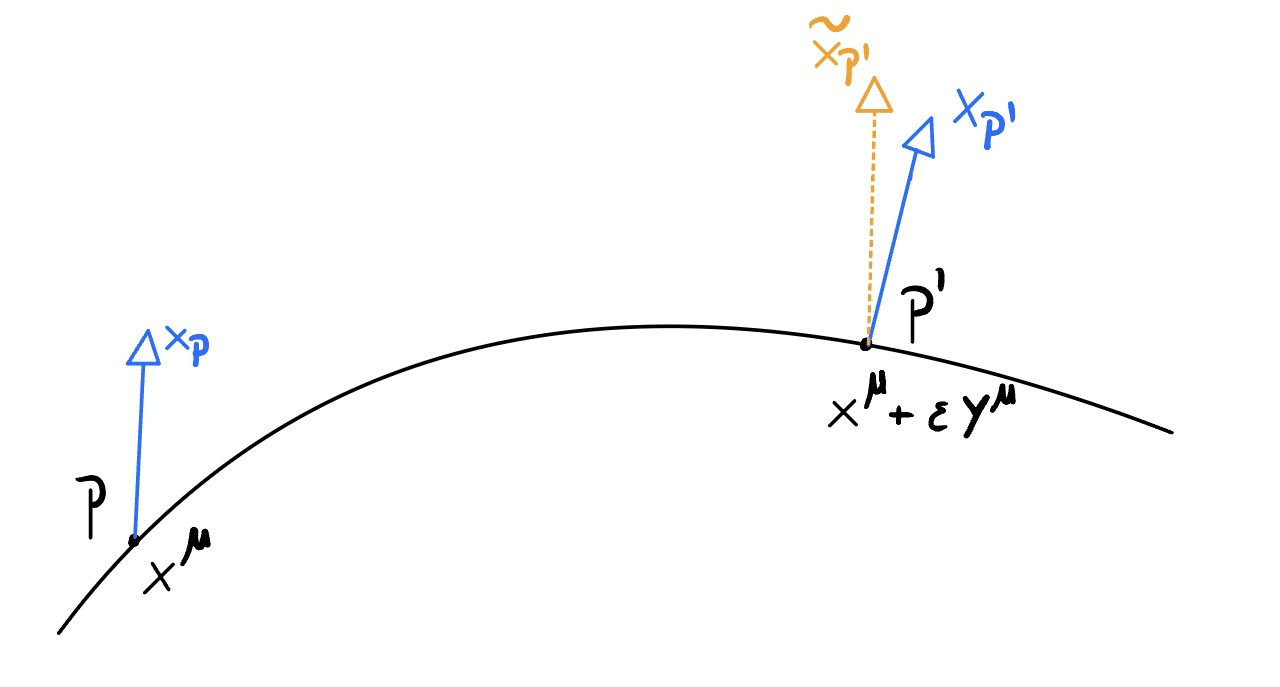
\includegraphics[scale=0.15]{Chapitres/5. Géodésiques/Images/transport parallèle.jpg} 
\end{center}

On se rappelle qu'on pouvait caractériser la connexion par le transport parallèle :
\begin{equation}
    \nabla_{Y}X = \lim_{\varepsilon \rightarrow 0}\frac{\overset{\sim}{X}(x + \varepsilon Y) - X(x+\varepsilon Y)}{\varepsilon} = 0
\end{equation}
Cette équation est nulle si et seulement si $\overset{\sim}{X}_{P'} = X_{P'}$. Le champs de vecteurs $U$ est donc bien transporté parallèlement à lui-même si et seulement si 
\begin{equation}
    \nabla_{U}U =0 
\end{equation}
Comme par la définition \ref{def:géodésiques1}. En termes de composantes,  $U = U^{\beta}\partial_{\beta}$ et donc
\begin{equation}
U^{\beta}\nabla_{\beta}U^{\alpha} = 0
\end{equation}
Autrement dit, en développant par la relation \ref{def: dérivée covariante vecteur}
\begin{align}
    &\frac{\td x^{\beta}}{\td \tau} (\partial_{\beta}U^{\alpha} + \Gamma^{\alpha}_{\beta \gamma}U^{\gamma}) = 0\\
     &\textcolor{blue}{\frac{\td x^{\beta}}{\td \tau}\frac{\partial}{\partial x^{\beta}}}\left(\frac{\td x^{\alpha}}{\td \tau}\right) + \Gamma^{\alpha}_{\beta \gamma}\frac{\td x^{\beta}}{\td \tau}\frac{\td x^{\gamma}}{\td \tau} = 0\\
     & \textcolor{blue}{\frac{\td }{\td \tau}}\frac{\td x^{\alpha}}{\td \tau} + \Gamma^{\alpha}_{\beta \gamma} \frac{\td x^{\beta}}{\td \tau}\frac{\td x^{\gamma}}{\td \tau}= 0\\
\end{align}

On obtient finalement l'\emph{équation des géodésique}s qui est aussi appelé équation des courbes \emph{auto-parallèles}:


\begin{equation}
    \boxed{\frac{\td^2x^{\alpha}}{\td\tau^2} + \Gamma^{\alpha}_{\beta \gamma}\frac{\td x^{\beta}}{\td \tau}\frac{\td x^{\gamma}}{\td \tau} = 0}
    \label{eq:géodésique} 
\end{equation}

\subsection{L'équation des géodésiques en absence de gravitation dans un référentiel inertiel}
En absence de gravitation (en relativité restreinte), $\Gamma^{\alpha}_{\mu \nu} = 0$ identiquement et donc
\begin{equation}
    \frac{\td^2x^{\alpha}}{\td\tau^2} = 0
    \label{eq:droite Minkowski}
\end{equation}
C'est l'équation d'une droite (Minkowskienne), c'est-à-dire une trajectoire du type
\begin{equation}
    x^\alpha (\tau) = v^\alpha \tau + x_0^\alpha
\end{equation}
où $v,x_0 \in \R^{3,1}$. Ce sont également les trajectoires libres usuels (en absence de gravitation et d'autres forces). En effet, l'équation \ref{eq:droite Minkowski} correspond aussi à la première loi de Newton transposée en relativité restreinte. \\
\\
Dans l'espace-temps de Minkowski, 
\begin{equation}
    \td \tau = \sqrt{\td t^2 - \td x^2 -\td y^2 - \td z^2}
\end{equation}
et donc 
\begin{equation}
    \frac{\td \tau}{\td t} = \sqrt{1- \vect{v}^2}
\end{equation}
On peut définir la quadri-vitesse selon
\begin{equation}
    u^\alpha = \frac{\td x^\alpha}{\td \tau} = \frac{\td}{\td \tau} (\td t,\td x,\td y,\td z) = \frac{1}{\sqrt{1-\vect{v}^2}} (1,\vect{v})
\end{equation}
En particulier, dans le référentiel propre de la particule, $u = (1,0,0,0)$. La quadri-accélération vaut
\begin{equation}
    a^\alpha = \frac{\td u^\alpha}{\td \tau} = \frac{\td t}{\td \tau}\frac{\td}{\td t} \lt \frac{(1,\vect{v})}{\sqrt{1-\vect{v}^2}} \rt
\end{equation}
notons $v=\lvert \vect{v} \rvert$, $\dot{v} = \frac{\td}{\td t} \lvert \vect{v} \rvert$ ainsi que $\vect{a} = \frac{\td \vect{v}}{\td t}$. On trouve alors
\begin{equation}
    a^\alpha = \lt \frac{v \dot{v}}{(1-v^2)^2}, \frac{v \dot{v}}{(1-v^2)^2} \vect{v} + \frac{1}{1-v^2} \vect{a}\rt
\end{equation}
On trouve donc que les solutions de $a^\alpha = \dfrac{\td^2 x^\alpha}{\td \tau^2} = 0$ :
\begin{equation}
    \left\{
    \begin{array}{l}
        v = 0 \quad \text{ou} \quad \dot{v} = 0  \\
        \vect{a} = 0
    \end{array}
    \right.
\end{equation}
Soit que la vitesse $\vect{v}$ de la particule est constante dans tout référentiel inertiel : la trajectoire d'une particule libre est une droite. Ceci confirme donc notre discussion ci-avant. Remarquons à présent que conformément au principe d'équivalence, \ref{eq:droite Minkowski} représente (localement) une trajectoire libre en espace-temps courbe (donc en présence de gravitation), dans un référentiel localement inertiel. \\
De la même manière, par le principê d'équivalence, \ref{eq:géodésique} représente (localement) autant la trajectoire libre dans un espace-temps courbe (donc en présence de gravitation), qu'une trajectoire libre dans un espace-temps plat, dans un référentiel non-inertiel.
\subsection{L'équation des géodésiques en absence de gravitation dans un référentiel non-inertiel}
Prenons la trajectoire d'une particule libre dans un espace-temps plat et dans un référentiel inertiel, dont l'équation du mouvement s'écrit 
\begin{equation*}
    \frac{\td^2x^{\hat{\alpha}}}{\td\tau^2} = 0
\end{equation*}
Dans un référentiel quelconque (donc non-inertiel), cette expression se transforme selon

On sait que 
\begin{align}
    \frac{\td x^{\hat{\alpha}}}{\td \tau} = \frac{\partial x^{\hat{\alpha}}}{\partial x^{\alpha}}\frac{\td x^{\alpha}}{\td\tau}
\end{align}
En différenciant une seconde fois :
\begin{align}
    0 = \frac{\td ^2x^{\hat{\alpha}}}{\td \tau^2} &= \frac{\td }{\td \tau}\left(\frac{\td x^{\alpha}}{\td \tau}\frac{\partial x^{\hat{\alpha}}}{\partial x^{\alpha}}\right)\\
    &= \frac{\td ^2x^{\alpha}}{\td \tau^2}\frac{\partial x^{\hat{\alpha}}}{\partial x^{\alpha}} + \frac{\td x^{\alpha}}{\td \tau}\frac{\td }{\td \tau}\left(\frac{\partial x^{\hat{\alpha}}}{\partial x^{\alpha}}\right)\\
    &= \frac{\td ^2x^{\alpha}}{\td \tau^2}\frac{\partial x^{\hat{\alpha}}}{\partial x^{\alpha}} + \frac{\td x^{\alpha}}{\td \tau}\frac{\td x^{\beta}}{\td \tau} \frac{\partial}{\partial x^{\beta}}\left(\frac{\partial x^{\hat{\alpha}}}{\partial x^{\alpha}}\right)\\
    &=\frac{\td ^2x^{\alpha}}{\td \tau^2}\frac{\partial x^{\hat{\alpha}}}{\partial x^{\alpha}} + \frac{\td x^{\alpha}}{\td \tau}\frac{\td x^{\beta}}{\td \tau} \frac{\partial^2 x^{\hat{\alpha}}}{\partial x^{\alpha}\partial x^{\beta}}
\end{align}
On obtient alors
\begin{align}
    0 = \frac{\partial x^{\mu}}{\partial x^{\hat{\alpha}}} \frac{\td ^2x^{\hat{\alpha}}}{\td \tau^2}&= \frac{\partial x^{\mu}}{\partial x^{\hat{\alpha}}} \left(\frac{\td ^2x^{\alpha}}{\td \tau^2}\frac{\partial x^{\hat{\alpha}}}{\partial x^{\alpha}} + \frac{\td x^{\alpha}}{\td \tau}\frac{\td x^{\beta}}{\td \tau} \frac{\partial^2 x^{\hat{\alpha}}}{\partial x^{\alpha}\partial x^{\beta}}\right)=0\\
    &=  \delta^{\mu}_{\alpha}\frac{\td ^2x^{\alpha}}{\td \tau^2} + \frac{\partial^2 x^{\hat{\alpha}}}{\partial x^{\alpha}\partial x^{\beta}}\frac{\partial x^{\mu}}{\partial x^{\hat{\alpha}}} \frac{\td x^{\alpha}}{\td \tau}\frac{\td x^{\beta}}{\td \tau}=0\\
    &= \frac{\td ^2x^{\mu}}{\td \tau^2} + \frac{\partial^2 x^{\hat{\alpha}}}{\partial x^{\alpha}\partial x^{\beta}}\frac{\partial x^{\mu}}{\partial x^{\hat{\alpha}}} \frac{\td x^{\alpha}}{\td \tau}\frac{\td x^{\beta}}{\td \tau}=0
\end{align}
En posant
\begin{equation}
    \gamma^\mu_{\alpha\beta} = \frac{\partial^2 x^{\hat{\alpha}}}{\partial x^{\alpha}\partial x^{\beta}}\frac{\partial x^{\mu}}{\partial x^{\hat{\alpha}}}
\end{equation}
On peut réécrire une équation analogue à l'équation des géodésiques pour le cas d'un espace-temps plat et dans un référentiel quelconque :
\begin{equation}
    \frac{\td ^2x^{\mu}}{\td \tau^2} + \gamma^\mu_{\alpha\beta} \frac{\td x^{\alpha}}{\td \tau}\frac{\td x^{\beta}}{\td \tau}=0
\end{equation}
Le facteur $\gamma$ joue donc le rôle des forces inertielles fictives résultantes du choix d'un référentiel non-inertiel. 
\begin{exerc}
    Montrez que dans le cas général d'un espace-temps courbe, 
    \begin{equation}
        \boxed{\Gamma^{\mu}_{\alpha \beta} = \frac{\partial^2 x^{\hat{\alpha}}}{\partial x^{\beta}\partial x^{\alpha}}\frac{\partial x^{\mu}}{\partial x^{\hat{\alpha}}} }
        \label{eq: Coefficients en dérivées}
    \end{equation}
    Ce qui confirme que les coefficients de connexion (et par extension, la métrique) capturent les forces fictives d'inertie, et par le principe d'équivalence, la gravitation.
\end{exerc}
Donnons un mode opératoire pour prouver cette égalité
\begin{enumerate}
    \item On montre que les deux objets coïncident dans un système de coordonnées particulier. 
    \item On montre que les deux côtés se transforment de la même manière sous changement général de coordonnées.
\end{enumerate}
\subsection{Paramétrisation affine}
Pour dériver l'équation des géodésiques, nous avions utilisés le temps propre comme paramétrisation de la courbe. Il s'avère que \ref{eq: Coefficients en dérivées} n'est pas invariant sous reparamétrisation de la courbe. Il est donc intéressant d'étudier une forme générale de l'équation des géodésiques où le temps propre est remplacé par un paramètre arbitraire $\lambda$. Considérons donc le changement de paramétrisation
\begin{equation*}
    x^\mu (\lambda) \to x^\mu(\tau) = x^\mu(\tau(\lambda))
\end{equation*}
Étant donné
\begin{equation}
    \frac{\td x^{\mu}}{\td \lambda} = \frac{\td \tau}{\td \lambda}\frac{\td  x^{\mu}}{\td \tau}
\end{equation}
et l'équation des géodésiques dans la paramétrisation en temps propre, on peut calculer :
\begin{align}
    \frac{\td ^2 x^{\mu}}{\td \lambda ^2} &= \frac{\td }{\td \lambda}\left(\frac{\td \tau}{\td \lambda}\frac{\td  x^{\mu}}{\td \tau}\right)\\
    & = \frac{\td ^2 \tau}{\td \lambda ^2}\frac{\td  x^{\mu}}{\td \tau} +  \frac{\td \tau}{\td \lambda} \frac{\td }{\td \lambda}\frac{\td  x^{\mu}}{\td \tau }\\
    &=\frac{\td ^2 \tau}{\td \lambda ^2}\textcolor{blue}{\frac{\td  x^{\mu}}{\td \tau}} +  \frac{\td \tau}{\td \lambda} \frac{\td \tau}{\td \lambda}\textcolor{purple}{\frac{\td ^2 x^{\mu}}{\td \tau ^2}}\\
    &= \frac{\td ^2 \tau}{\td \lambda ^2}\textcolor{blue}{\frac{\td \lambda}{\td \tau}\frac{\td  x^{\mu}}{\td \lambda}} + \left(\frac{\td \tau}{\td \lambda}\right)^2\textcolor{purple}{\lt-\Gamma^{\mu}_{\alpha \beta}\frac{\td  x^{\alpha}}{\td \tau}\frac{\td  x^{\beta}}{\td \tau} \rt}\\
    &= \frac{\td ^2 \tau}{\td \lambda ^2}\frac{\td \lambda}{\td \tau}\frac{\td  x^{\mu}}{\td \lambda} - \Gamma^{\mu}_{\alpha \beta}\frac{\td  x^{\alpha}}{\td \lambda}\frac{\td  x^{\beta}}{\td \lambda}
\end{align}
On obtient donc la généralisation suivante :
\begin{align}
     \boxed{\frac{\td ^2 x^{\mu}}{\td \lambda ^2} + \Gamma^{\mu}_{\alpha \beta}\frac{\td  x^{\alpha}}{\td \lambda}\frac{\td  x^{\beta}}{\td \lambda} = \frac{\td ^2 \tau}{\td \lambda ^2}\frac{\td \lambda}{\td \tau}\frac{\td  x^{\mu}}{\td \lambda}}
     \label{eq:pour expliquer Morera v2}
\end{align}
Une observation curieuse est que cette équation se ramène à l'équation des géodésiques précédente si et seulement si $\lambda = a \lambda + b$. Autrement dit, l'équation des géodésiques est invariante sous la reparamétrisation
\begin{equation*}
    \tau \to \lambda = a\tau+b
\end{equation*}
Un tel paramètre est appelé \emph{paramètre affine}. Notons également que seul avec un tel paramètre, les droites Minkowskiennes correspondant à des mouvements libres en relativité restreinte s'expriment sous la forme \ref{eq:droite Minkowski}.
\begin{theoremframe}
    \begin{theorem}[Théorème de je ne sais pas à quoi ça sert]
        Soit une courbe $x^\alpha (\lambda)$ à vecteur tangent $U^\alpha$ satisfaisant 
        \begin{equation}
            \nabla_U U = g(\lambda) U
        \end{equation}
        Alors il existe un changement de paramétrisation (lisse) telle que l'équation des géodésiques est satisfaite, i.e.
    \begin{equation*}
        \nabla_U U = 0
    \end{equation*}
    \end{theorem}
\end{theoremframe}
\begin{proof}
    Il suffit de considérer le raisonnement inverse qui nous a emmené à \ref{eq:pour expliquer Morera v2}. On pose alors la reparamétrisation $\lambda \to \lambda' = \lambda'(\lambda)$:
    \begin{equation}
        g(\lambda) = \frac{\td^2 \lambda'}{\td \lambda^2} \frac{\td \lambda}{\td \lambda'}
    \end{equation}
    Réécrivant les variables vers quelque chose de compréhensible, notons la nouvelle variable $q$ et l'ancienne variable $t$. On trouve alors l'EDO
    \begin{equation}
        \ddot{q}(t) g(t) = \dot{q}(t)
    \end{equation}
    Avec la fonction lisse $g$. Celle-ci admet 
\end{proof}
\section{Géodésiques et principe variationnel}
On a vu précédemment qu'on pouvait définir le genre d'une courbe (à tout point) comme le genre de son vecteur tangent en ce point. Néanmoins, dans le cas général, le genre d'une courbe peut changer en fonction du point considéré. On montre ici que ce n'est pas le cas des géodésiques
\begin{theoremframe}
    \begin{propri}
        Le genre d'une géodésique est bien défini. Autrement dit, son genre ne peut pas changer le long de la courbe. En particulier, si $\lambda$ est un paramètre affine, la norme du vecteur tangent est une constante du mouvement.
        \begin{equation}
            \frac{\td}{\td\lambda}\lVert U \rVert^2 = 0
        \end{equation}
    \end{propri}
\end{theoremframe}
Nous monterons uniquement qu'une géodésique qui est de genre temps en un point l'est à tout point. La preuve se généralise de la même manière aux autres genres.
\begin{proof}
    Soit une géodésique à coordonnées $x^{\alpha}(\lambda)$. Par le théorème ah-je-sais-à-quoi-il-sert-maintenant de la section précédente, nous pouvons sans perte de généralité considérer que celle-ci est paramétrisée par un paramètre affine à vecteur tangent  $U^{\alpha} = \frac{\td x^{\alpha}}{\td\lambda}$. Notons que le genre de la courbe à un point donné ne dépend pas du choix de paramétrisation, et il suffit donc de montrer que le genre de la géodésique est bien défini pour la paramétrisation affine. On a par définition :
    \begin{align}
        \Vert  U \Vert ^2 =& g_{\mu \nu}U^{\mu}U^{\nu}\\
        =& g_{\alpha \beta}\frac{\td x^{\alpha}}{\td \lambda}\frac{\td x^{\beta}}{\td \lambda} = g_{\alpha\beta} \dot{x}^\alpha \dot{x}^\beta
    \end{align}

    On veut montrer que 
    \begin{equation}
        \frac{\td }{\td \lambda}\left(\Vert  U \Vert ^2\right)=0
    \end{equation}
    Muni de la propriété 
    \begin{equation*}
    \frac{\td}{\td \lambda} g_{\alpha\beta} = \frac{\td x^\mu}{\td \lambda} \pd_\mu g_{\alpha\beta} = U^\mu \pd_\mu g_{\alpha\beta}
    \end{equation*}
    on calcule :
    \begin{align}
        \frac{\td }{\td \lambda}\left(\Vert  U \Vert ^2\right)
        =&\frac{\td }{\td \lambda}\left(g_{\alpha \beta}\dot{x}^{\alpha}\dot{x}^{\beta} \right)\\
        =&\left(\dot{x}^{\mu}\partial_{\mu}g_{\alpha \beta}\right)\dot{x}^{\alpha}\dot{x}^{\beta}  + 2g_{\alpha \beta}\textcolor{blue}{\ddot{x}^{\alpha}}\dot{x}^{\beta}\\
        =&\left(\dot{x}^{\mu}\partial_{\mu}g_{\alpha \beta}\right)\dot{x}^{\alpha}\dot{x}^{\beta} + 2g_{\alpha \beta}\textcolor{blue}{\left(-\Gamma^{\alpha}_{\mu \nu}\dot{x}^{\mu}\dot{x}^{\nu}\right)} \dot{x}^{\beta}\\
        =&\partial_{\mu}g_{\alpha \beta}\dot{x}^{\mu}\dot{x}^{\alpha}\dot{x}^{\beta} - 2g_{\alpha \beta}\dot{x}^{\beta}\dot{x}^{\mu}\dot{x}^{\nu}\left[\frac{1}{2}g^{\alpha \theta}\left(\partial_{\mu}g_{\theta\nu} + \partial_{\nu}g_{\mu \theta}-\partial_{\theta}g_{\mu \nu}\right)\right]
    \end{align}
    Il suffit à présent de développer le second terme 
    \begin{align}
        \frac{\td }{\td \lambda}\left(\Vert  U \Vert ^2\right)
        =&\partial_{\mu}g_{\alpha \beta}\dot{x}^{\mu}\dot{x}^{\alpha}\dot{x}^{\beta} - \dot{x}^{\theta}\dot{x}^{\mu}\dot{x}^{\nu}\left(\partial_{\mu}g_{\theta\nu} + \partial_{\nu}g_{\mu \theta}-\partial_{\theta}g_{\mu \nu}\right)\\
        =&\partial_{\mu}g_{\textcolor{blue}{\theta} \textcolor{blue}{\nu}}\dot{x}^{\mu}\dot{x}^{\textcolor{blue}{\theta}}\dot{x}^{\textcolor{blue}{\nu}} - \dot{x}^{\theta}\dot{x}^{\mu}\dot{x}^{\nu}\left(\partial_{\mu}g_{\theta\nu} + \partial_{\nu}g_{\mu \theta}-\partial_{\theta}g_{\mu \nu}\right)\\
        =&\dot{x}^{\theta}\dot{x}^{\mu}\dot{x}^{\nu}\left( \textcolor{red}{\partial_{\mu}g_{\theta\nu}} -\textcolor{red}{\partial_{\mu}g_{\theta\nu}} - \partial_{\nu}g_{\mu \theta}+\partial_{\theta}g_{\mu \nu} \right)\\
        =&\dot{x}^{\theta}\dot{x}^{\mu}\dot{x}^{\nu}\left( - \partial_{\nu}g_{\mu \theta}+\partial_{\theta}g_{\mu \nu} \right)\\
    \end{align}
    Le terme en la métrique est antisymétrique en $\nu$ et $\theta$, alors que le terme en les $\dot{x}$ en est symétrique : la contraction s'annule. 
\end{proof}
\begin{rmk}
    Le temps propre d'une courbe n'est défini que pour une courbe causale. De plus, pour les intervalles de type temps, le temps propre est identiquement nul (comme $\td s^2 = 0$) et n'est donc pas un paramètre adapté. Pour prouver le résultat ci-dessus, nous devons donc d'abord montrer que l'équation des géodésiques reste valable dans ces cas pour un paramètre affine, qui à présent sera défini comme un paramètre coupant la courbe en morceaux équidistants. La propriété principale des paramètres affines reste valable : si $\lambda$ est un paramètre affine alors $a\lambda +b$ en est un aussi.
\end{rmk}
Nous avons jusqu'ici utilisé la première version de la définition \ref{def:géodésiques1}, en définissant les géodésiques comme des \emph{courbes auto-parallèles}. Nous allons à présent nous intéresser à la deuxième formulation, en montrant qu'ils correspondent également à des \emph{courbes extrémales}. \\
\\
Nous avions vu que la longueur Minkowskienne en espace-temps plat mesurée le long de courbes causales est extrémale (maximale dans le cas présent) par la droite. Nous allons généraliser ce résultat à un espace Lorentzien quelconque $(\mathcal{M},g)$ muni de la connexion de Levi-Civita, par analogie des géodésiques comme généralisation des lignes droites.
\begin{theoremframe}
    \begin{propri}
    L'équation des géodésiques découle d'un principe variationnel : soit une courbe $x^{\mu}(\lambda)$ de genre temps. La fonctionnelle 
    \begin{equation}
        \tau[x^\mu] = \int \td\tau = \int^{\lambda_2}_{\lambda_1}\sqrt{-g_{\mu \nu}\frac{\td x^{\mu}}{\td\lambda}\frac{\td x^{\nu}}{\td\lambda}}\td\lambda
        \label{eq:principe variationnel géodésiques}
        \end{equation}
        est extrémisée par les géodésiques temporelles, c'est à dire que
        \begin{equation}
            \delta \tau = 0 \iff \frac{\td ^2 x^{\alpha}}{\td \tau^2} + \Gamma^{\alpha}_{\beta \gamma}\frac{\td x^{\beta}}{\td \tau}\frac{\td x^{\gamma}}{\td \tau} = 0
        \end{equation}
    \end{propri}
\end{theoremframe}

\begin{proof} La preuve se fait en deux étapes
    \subsubsection{Étape 1 : réécriture de la fonctionnelle}
    Posons
    \begin{equation}
        f = g_{\mu \nu}\frac{\td x^{\mu}}{\td \lambda}\frac{\td x^{\nu}}{\td \lambda}
    \end{equation}
    Alors, la fonctionnelle se réécris
    \begin{equation}
        \tau =\int^{\lambda_2}_{\lambda_1}\sqrt{-f}\td\lambda
    \end{equation}
    et sa variation s'écrit
    \begin{equation}
        \delta \tau = \int -\frac{1}{2}(-f)^{-\frac{1}{2}}\delta f \td \lambda
    \end{equation}
    Notons que l'action \ref{eq:principe variationnel géodésiques} est invariante sous reparamétrisation $\lambda \rightarrow \lambda'(\lambda)$. Choisissons donc comme paramétrisation le temps propre. On trouve alors
    \begin{equation}
        f = g_{\mu \nu}\frac{\td x^{\mu}}{\td \tau}\frac{\td x^{\nu}}{\td \tau}= \frac{\td s^2}{\td \tau ^2}= -\frac{\td \tau^2}{\td \tau ^2} = -1
    \end{equation}
    Ce qui implique que la variation du temps propre est 
    \begin{equation}
        \delta \tau = -\frac{1}{2}\int \delta f \td\tau \quad \text{donc soit} \quad \delta \tau = 0 \iff \delta f=0
    \end{equation}
    Les points stationnaires de la fonctionnelle \ref{eq:principe variationnel géodésiques} sont donc les mêmes que ceux de la fonctionnelle suivante 

    \begin{equation}
        \boxed{I[x^\mu] = \frac{1}{2}\int g_{\mu \nu} \frac{\td x^{\mu}}{\td \tau}\frac{\td x^{\nu}}{\td \tau} \td \tau \equiv \int \mathcal{L}_t \td \tau}
        \label{eq:action I}
    \end{equation}
    \subsubsection{Équations du mouvement de la nouvelle fonctionnelle}
    Sous cette forme, les équations d'Euler-Lagrange s'écrivent
    \begin{equation}
        \frac{\delta I}{\delta x^{\mu}} = 0 \iff \frac{\td }{\td \tau}\frac{\partial \mathcal{L}}{\partial \dot{x}^{\mu}} - \frac{\partial \mathcal{L}}{\partial {x}^{\mu}} = 0
    \end{equation}
Le lagrangien est
\begin{equation}
    \mathcal{L} = \frac{1}{2}g_{\alpha \beta}\dot{x}^{\alpha}\dot{x}^{\beta} 
\end{equation}
Notons que cette équation dépend bien implicitement de $x^\mu$ à travers la métrique. Calculons le termes des équations d'Euler-Lagrange :
\begin{align}
    \frac{\partial \mathcal{L}}{\partial x^{\mu}}& =\frac{1}{2}\partial_{\mu}g_{\alpha \beta}\dot{x}^{\alpha}\dot{x}^{\beta}\\
    \frac{\partial \mathcal{L}}{\partial \dot{x}^{\mu}} &= \frac{1}{2}g_{\alpha \beta}\frac{\partial \dot{x}^{\alpha}}{\partial \dot{x}^{\mu}}\dot{x}^{\beta} + \frac{1}{2}g_{\alpha \beta}\dot{x}^{\alpha}\frac{\partial \dot{x}^{\beta}}{\partial \dot{x}^{\mu}} = g_{\alpha \beta} \dot{x}^{\beta}
\end{align}
Et
\begin{align}
    \frac{\td}{\td\lambda}\frac{\partial \mathcal{L}}{\partial \dot{x}^{\mu}} &= \frac{\td}{\td\lambda}(g_{\alpha \beta}\dot{x}^{\beta})\\
    &= \dot{x}^{\gamma} \partial_{\gamma}g_{\alpha \beta}\dot{x}^{\beta} + g_{\alpha \beta}\ddot{x}^{\beta}
\end{align}
En distribuant la dérivée et en développant $\frac{\td}{\td \lambda} =\dot{x}^\mu \pd_\mu$ par la règle de la chaîne. En combinant, on trouve finalement
\begin{align}
    \partial_{\alpha}g_{\mu \nu}\dot{x}^{\alpha}\dot{x}^{\nu} + g_{\mu \nu}\ddot{x}^{\nu} - \frac{1}{2}\partial_{\mu}g_{\alpha \nu}\dot{x}^{\alpha}\dot{x}^{\nu} &= 0 \\
    \intertext{Or, comme}
    \partial_{\textcolor{purple}{\alpha}}g_{\mu \textcolor{blue}{\nu}}\dot{x}^{\textcolor{purple}{\alpha}}\dot{x}^{\textcolor{blue}{\nu}} = \frac{1}{2} \lt\partial_{\textcolor{purple}{\alpha}}g_{\mu \textcolor{blue}{\nu}} \dot{x}^{\textcolor{purple}{\alpha}}\dot{x}^{\textcolor{blue}{\nu}} + \partial_{\textcolor{purple}{\nu}}g_{\mu \textcolor{blue}{\alpha}}\dot{x}^{\textcolor{blue}{\alpha}}\dot{x}^{\textcolor{purple}{\nu}} \rt
    \intertext{On peut contracter les équations du mouvement avec $g^{\mu \beta}$}
    g^{\mu \beta} \left[\frac{1}{2}\partial_{\alpha}g_{\mu \nu} \dot{x}^{\alpha}\dot{x}^{\nu} + \frac{1}{2}\partial_{\nu}g_{\mu \alpha}\dot{x}^{\alpha}\dot{x}^{\nu} + g_{\mu \nu}\ddot{x}^{\nu} \right]  &- \frac{1}{2}\partial_{\mu}g_{\alpha \nu}\dot{x}^{\alpha}\dot{x}^{\nu} = 0\\
    \ddot{x}^{\beta} + \frac{1}{2}g^{\mu \beta} \left(\partial_{\alpha}g_{\mu \nu} + \partial_{\nu}g_{\mu \alpha} - \partial_{\mu}g_{\alpha \beta}\right) \dot{x}^{\alpha}\dot{x}^{\nu} &= 0
\end{align}
On peut directement définir les coefficients de connexion via l'expression \ref{Connexion de Levi-Civita}.
\begin{equation}
    \frac{d^2x^{\alpha}}{d\lambda^2 } + \Gamma^{\mu}_{\alpha \beta} \frac{dx^{\alpha}}{d\lambda} \frac{dx^{\beta}}{d\lambda} = 0
\end{equation}
Les courbes auto-parallèles et les courbes qui extrémisent le temps propre sont les mêmes et sont valables pour tout $\Gamma$.
\end{proof}
Formulons une série de commentaires sur cette propriété :
\begin{enumerate}

    \item La fonctionelle $\tau[x^\mu]$ est invariante sous reparamétrisation alors que $I[x^\mu]$ ne l'est pas. Ce n'est que lorsque les courbes sont paramétrés par un paramètre affine que les points stationnaires des actions [\ref{eq:temps propre}] et [\ref{eq:action I}] coïncident. En effet, si les courbes sont paramétrés par $\lambda = a\tau + b$  on obtient que  $\td\tau = a \td\lambda$ et 
    \begin{equation}
    \frac{\td}{\td\tau} = \frac{\td\lambda}{\td\tau}\frac{\td}{\td\lambda} = \frac{1}{a}\frac{\td}{\td\lambda}
    \end{equation}
    La fonctionelle $I$ se transforme donc sous un paramètre affine selon
    \begin{equation}
        I \to \frac{1}{2}\int g_{\mu \nu}\frac{1}{a^2}\frac{\td x^{\mu}}{\td\lambda}\frac{\td x^{\nu}}{\td\lambda} a \,\td\lambda = \frac{1}{a}I
    \end{equation}
    On voit que manifestement, $I$ n'est pas invariant sous changement de paramétrisation, et n'aura en général plus les mêmes points stationnaires.
    \item Pour une conexion de Levi-Civita, les courbes auto-parallèles coïncident avec les courbes extrémales (maximales) du temps propre. Ceci est important pour que le principe d'équivalence soit vrai.
    \item L'équation des géodésiques sont des équations du second ordre. Une géodésique est donc caractérisé par deux données initiales comme par exemple :
    \begin{equation}
        x^\mu(P) \quad \text{et} \quad \frac{\td x^\mu}{\td \lambda} (P)
    \end{equation}
    ou encore
    \begin{equation}
        x^\mu(P) \quad \text{et} \quad x^\mu(Q)
    \end{equation}
    En particulier, s'il existe un point $P$ tel que deux géodésiques possèdent le même vecteur tangent en ce point, alors elles sont identiques (unicité de la solution au problème de Cauchy). 
    \item En un point, il peut y avoir trois types différents de géodésique.
\end{enumerate}
En conclusion à cette partie, les observateurs en chute libre (observateurs localement inertiels) suivent une géodésique. Leur quadri-accélération est nulle. En effet, ceux-ci sont supposés uniquement soumis à la gravitation, et se meuvent donc en chute libre dans un espace-temps courbe selon le principe d'équivalence.

\section{Géodésiques nulles*}
\section{Observateurs localement inertiels revisités}
Nous allons retravailler la formulation du principe d'équivalence dans le cadre des géodésiques (qui sont les RLI prédits par celui-ci).
\begin{theoremframe}
    \begin{theorem}
        Soit une géodésique de genre temps. Il existe au moins un système de coordonnée $\{x^{\mu}\} = \{x^0 , x^k\}$ tel que le long de la géodésique :
        \begin{enumerate}
            \item $x^k = 0$
            \item $\tau = x^0$ 
            \item $g_{\alpha \beta}(x^0, 0) = \eta_{\alpha \beta}$
            \item $\Gamma^{\alpha}_{\beta \gamma}(x^0, 0) = 0$
        \end{enumerate}
    \end{theorem}
\end{theoremframe}
\begin{proof}
    Une partie de la preuve sera abordée en séance d'exercices.
    \subsubsection{Preuve de la propriété 1.}
    Soit $y^{\mu}(\tau)$ une géodésique. Son équation est donné par 
    \begin{equation}
        \left\{
        \begin{array}{l}
            y^0 = y^0(\tau)\\
            y^{i} = y^{i}(\tau)
        \end{array}
        \right.
    \end{equation}
    Comme le vecteur tangent de la géodésique ne s'annule jamais (comme c'est une géodésique temporelle), nous pouvons appliquer le \emph{théorème de la fonction implicite}. Celui-ci assure qu'on peut inverser localement l'équation $y^0 = y^0(\tau)$ en tout point tel que $\tau = \tau(y^0)$ (ainsi, on peut l'inverser globalement). En injectant cette relation dans la partie spatiale : 
    \begin{equation}
        y^{i} = y^{i}(\tau(y^0)) = y^{i}(y^0)
    \end{equation}
    On peut introduire un nouveau système de coordonnée tel que
    \begin{equation}
        \left\{
        \begin{array}{l}
            \Bar{x}^k = y^k - y^k(y^0)=0\\
            \Bar{x}^0 = y^0
        \end{array}
        \right.
    \end{equation}
    Ceci est valable pour tout observateur.

    \subsubsection{Preuve de la propriété 2.}
    Le temps propre est défini par $\td \tau ^2 = -\td s^2 = -g_{\mu \nu}\td x^{\mu} \td x^{\nu}$. Le long d'une géodésique, dans les coordonnées $\Bar{x}^k$ de la preuve précédente, on trouve
    \begin{equation}
        \td \tau ^2 = -g_{0 0}(\Bar{x}^0, 0)\td \Bar{x}^{0} \td \Bar{x}^{0}
    \end{equation}
    Donc $\tau = \tau(\Bar{x}^0)$. On cherche un nouveau système de coordonnées $x'^k$ tel que la propriété 1. reste satisfaite et l'équation $\td \tau^2 = - g_{00}(\Bar{x}^0)(\td \Bar{x}^0)^2$ devient $(\td x'^0)^2$. Comme la métrique dépend uniquement de $\Bar{x}^0$, il suffit d'effectuer la transformation
    \begin{equation}
        \left\{
        \begin{array}{l}
            x'^0 = \tau(\Bar{x}^0)\\
            x'^k = \Bar{x}^k
        \end{array}
        \right.
    \end{equation}
    Alors le temps propre le long de la géodésique $x'^{\mu} = x'^{\mu}(\tau)$ est $\tau = x'^{0}$.

    \subsubsection{Preuve de la propriété 3.}
    Le système de coordonnées précédent implique directement que la composante temporelle de la métrique $g_{00}$ se ramène à $-1$ dans le système de coordonnées $x'^\mu$. Nous cherchons donc un nouveau système de coordonnées $\Tilde{x}^\mu$ dans lequel les conditions \emph{(i)}, \emph{(ii)} et \emph{(iii)} sont satisfaites : 
    \begin{equation}
        \left\{
        \begin{array}{l}
            x'^0 = \Tilde{x}^0 + L\indices{^0_k}(\Tilde{x}^0) \Tilde{x}^k\\
            x'^k = \tilde{x}^k
        \end{array}
        \right.
    \end{equation}
    La condition \emph{(i)} reste manifestement vérifiée. La condition \emph{(ii)} impose 
    \begin{equation}
        \td \tau^2 = - g_{\tilde{0} \tilde{0}} (\td \tilde{x}^0)^2
    \end{equation}
    Par la loi de transformation de la métrique :
    \begin{align}
        \tilde{g}_{0 0} = \frac{\pd x^{\mu'}}{\pd \tilde{x}^0} \frac{\pd x^{\nu'}}{\pd \tilde{x}^0} g_{\mu'\nu'} = \dots =  g_{0'0'}
    \end{align}
    D'après un petit calcul que vous pouvez vérifier vous-même (similaire à la procédure ci-dessous). Imposons donc que la condition \emph{(iii)} soit également respectée
    \begin{align}
        \tilde{g}_{0i} &= \left. \frac{\pd x^{\mu'}}{\pd \tilde{x}^0} \frac{\pd x^{\nu'}}{\pd \tilde{x}^i}g_{\mu'\nu'} \right|_{\tilde{x}^k =0}\\
        & = \blue{\frac{\pd x^{0'}}{\pd \tilde{x}^0}} \frac{\pd x^{0'}}{\pd \tilde{x}^i}g_{0'0'} + \blue{\frac{\pd x^{0'}}{\pd \tilde{x}^0} }\gray{\frac{\pd x^{j'}}{\pd \tilde{x}^i}}g_{0'j'} +\purple{\frac{\pd x^{j'}}{\pd \tilde{x}^0}} \frac{\pd x^{0'}}{\pd \tilde{x}^i}g_{j'0'} + \purple{\frac{\pd x^{j'}}{\pd \tilde{x}^0}} \frac{\pd x^{k'}}{\pd \tilde{x}^i}g_{j'k'}
        \intertext{Où les termes en rouge s'annulent en considérant la transformation choisie. Les termes en bleu donnent 1 et le terme en gris donne $\delta^{j'}_i$.}
        &= \frac{\pd x'^{0}}{\pd \tilde{x}^i}g'_{00} +  g'_{0i} = -L\indices{^{0}_i} +  g'_{0i}
    \end{align}
    Nous pouvons ainsi imposer la condition :
    \begin{equation}
        L\indices{^0_i}(\tilde{x}^0) = \left. g'_{0i} \right|_{x'^k = 0}
    \end{equation}
    Pour que la métrique se simplifie selon $\left. \tilde{g}_{0i} \right|_{\tilde{x}^k = 0} = 0$. Il reste donc à diagonaliser $\tilde{g}_{ij}$. Considérons donc une nouvelle base de coordonnées\footnote{J'ai malheureusement épuisé mon arsenal de symboles sympas : good luck with this shit} $\{\mathfrak{z}^\mu \}$ tel que
    \begin{equation}
        \left\{
        \begin{array}{l}
            \tilde{x}^0 = \mathfrak{z}^0\\
            \tilde{x}^k = L\indices{^k_m}(\mathfrak{z}^0) \cdot \mathfrak{z}^m
        \end{array}
        \right.
    \end{equation}
    On peut toujours diagonaliser la matrice symétrique $\tilde{g} \to \mathfrak{g}$ par une matrice orthogonale $L$. Ensuite, nous pouvons normaliser séparément les $\mathfrak{z}^i \to \lambda^{(i)} \mathfrak{z}^i $ pour que ces coefficients soient égaux à 1\footnote{Notons que ceci ne modifiera pas les propriétés \emph{(i)} et \emph{(ii)}.}. Ceci conclut la preuve de la propriété \emph{(iii)}. 
\subsubsection{Preuve de la propriété 4.}
La preuve sera effectué en TP. Notons néanmoins que la preuve nécessitera le fait que la courbe $\mathfrak{z}^\mu(\mathfrak{z}^0)$ satisfait à l'équation des géodésiques.
\end{proof}
Notons que les propriétés \emph{(i)}-\emph{(iii)} n'ont pas nécessité l'hypothèse que la courbe est une géodésique. Elles restent donc vrai pour un observateur acceléré. N
\section{La limite Newtonienne}
Dans la limite Newtonienne (où $v \ll c$), nous aimerions imposer que l'équation des géodésiques se ramène à la loi de gravitation Newtonienne. Soit donc l'équation des géodésiques dans une métrique Lorentzienne arbitraire (courbe)
\begin{equation}
    \frac{d^2x^{\mu}}{d\tau^2} + \Gamma^{\mu}_{\alpha \beta}\frac{dx^{\alpha}}{d\tau}\frac{dx^{\beta}}{d\tau} = 0
\end{equation}
Dans cette limite, nous souhaitons retrouver 
\begin{equation}
    \sum \vect{F} = m\vect{a} = m\vect{g} = -m\vect{\nabla}\Phi
\end{equation}
où $\Phi$ est le potentiel gravitationnel :
\begin{equation}
\left\{
\begin{array}{l}
\Vec{g} = -\frac{GM}{r^2}.\Vec{1_{r}}\\
\Phi = \frac{GM}{r}
\end{array}
\right.
\end{equation}
En composantes, nous pouvons réécrire ceci comme
\begin{equation}
    \frac{d^2x^{i}}{dt^2} = -\partial^{i}\Phi
\end{equation}

\subsection{Gravitation linéarisée et limite newtonienne}
La limite Newtonienne, également appelée la gravitation linéarisée se définit comme suit :
\begin{theoremframe}
    \begin{defi} 
    La limite Newtonienne est
    \begin{enumerate}
        \item $\dfrac{\td x^{i}}{\td t} \ll c = 1$
        \item $g_{\mu \nu} = \eta_{\mu \nu} + h_{\mu \nu} + O(h^2)$ où $h$ représente une petite correction à la métrique plate. 
        \item $\partial_0 g_{\mu \nu} = 0$ i.e. le champ gravitationnel est statique (ne change pas dans le temps). Cela signifie aussi qu'aucune coordonnée ne dépend du temps. 
    \end{enumerate}
    \end{defi}
\end{theoremframe}
On va implémenter ces 3 conditions dans l'équation des géodésiques. Considérons $x^0 = ct$. Par \textit{(1)}, on a que 
\begin{align}
    \frac{dx^{i}}{dt} = \frac{dx^{i}}{dx^0} \ll 1 \implies \frac{dx^{i}}{d\tau} \ll \frac{dx^{0}}{d\tau}
\end{align}
Les termes en $\dfrac{dx^{i}}{d\tau}$ sont donc d'ordre supérieur et seront négligés dans la suite.
\begin{equation}
     \frac{\td ^2x^{\mu}}{\td \tau^2} + \Gamma^{\mu}_{0 0}\left(\frac{\td x^{0}}{\td \tau}\right)^2 +\dots = 0
\end{equation}
Que vaut $\Gamma^{\mu}_{0 0}$?
\begin{align}
    \Gamma^{\mu}_{0 0} &= \frac{1}{2}g^{\alpha \mu}(\partial_0 g_{\alpha 0} + \partial_{0}g_{0\alpha} - \partial_{\alpha}g_{00})\\
    &= -\frac{1}{2}g^{\alpha \mu}\partial_{\alpha}g_{00}
\end{align}
Où les deux premiers termes s'annulent par \textit{(3)}. 
De plus, par \textit{(2)}, $g_{\mu \nu} = \eta_{\mu \nu} + h_{\mu \nu} + O(h^2)$.
\begin{equation}
    \Gamma^{\mu}_{0 0} =-\frac{1}{2}g^{\alpha \mu}\partial_{\alpha}h_{00}
\end{equation}
Si $g_{\mu \nu} = \eta_{\mu \nu} + h_{\mu \nu} +O(h^2)$, alors $g^{\mu \nu} = \eta^{\mu \nu} - h^{\mu \nu } +O(h^2)$ (via la relation $g^{-1} g = \mathrm{Id}$). On trouve alors
\begin{align}
    \Gamma^{\mu}_{0 0} &=-\frac{1}{2}(\eta^{\mu \alpha} - h^{\mu \alpha })\partial_{\alpha}h_{00}\\
    &= -\frac{1}{2}\eta^{\mu \alpha}\partial_{\alpha}h_{00}\\
\end{align}
car on néglige les termes en $h^2$. L'équation des géodésique à la limite newtonienne s'écrit donc
\begin{equation}
     \frac{\td ^2x^{\mu}}{\td \tau^2} -\frac{1}{2}\eta^{\mu \alpha}\partial_{\alpha}h_{00}\left(\frac{\td x^{0}}{\td \tau}\right)^2 = 0
\end{equation}
Pour $\mu = 0$ :
\begin{align}
     &\frac{\td ^2x^{0}}{\td \tau^2} -\frac{1}{2}\eta^{00}\partial_{0}h_{00}\left(\frac{\td x^{0}}{\td \tau}\right)^2 = 0\\
\end{align}
Par \textit{(3)}, on a que $\partial_{0}h_{00} =0$.
\begin{equation}
    \frac{\td ^2x^{0}}{\td \tau^2} = 0 \implies \frac{\td x^{0}}{\td \tau} = \text{cste}
\end{equation}
i.e. on retrouve que $t$ est un paramètre affine, et on impose $ct = \tau$.
Pour $\mu = i$ :
\begin{align}
     &\frac{\td ^2x^{i}}{\td \tau^2} -\frac{1}{2}\partial^{i}h_{00}\left(\frac{\td x^{0}}{\td \tau}\right)^2 = 0\\
\end{align}
Or, par la chaîne :
\begin{align}
    \frac{\td }{\td \tau} = \frac{\td x^{\mu}}{\td \tau} \partial_{\mu}& = \frac{\td x^{0}}{\td \tau} \partial_{0} + \frac{\td x^{k}}{\td \tau} \partial_{k}\\
    & \simeq \frac{\td x^{0}}{\td \tau} \partial_{0}
\end{align}
Par \textit{(1)}. On reparamétrise la courbe avec $x^0(\tau)$ :
\begin{align}
     \frac{\td^2 x^{i}}{\td \tau^2} &= \frac{\td \textcolor{purple}{x^{0}}}{\td \tau} \partial_{\textcolor{purple}{0}}\left( \frac{\td \textcolor{blue}{x^{0}}}{\td \tau} \frac{\td x^{i}}{\td \textcolor{blue}{x^0}}\right)\\
     &=\frac{\td x^{0}}{\td \tau} \frac{\td x^{0}}{\td \tau}\partial_{0}\left(\frac{\td x^{i}}{\td x^0}\right) \\
     &=\left(\frac{\td x^{0}}{\td \tau}\right)^2 \frac{\td }{\td x^0}\left(\frac{\td x^{i}}{\td x^0}\right)\\
     &=\left(\frac{\td x^{0}}{\td \tau}\right)^2 \frac{\td ^2 x^{i}}{\td (x^0)^2}
\end{align}
La composant $\mu = i$ s'écrit donc
 \begin{align}
     \left(\frac{\td x^{0}}{\td \tau}\right)^2 \frac{\td ^2 x^{i}}{\td (x^0)^2} -\frac{1}{2}\partial^{i}h_{00}\left(\frac{\td x^{0}}{\td \tau}\right)^2 = 0\implies \frac{\td ^2 x^{i}}{\td (x^0)^2} -\frac{1}{2}\partial^{i}h_{00}=0
\end{align}
On réstore $c$ à travers $x^0 = ct$ :

\begin{align}
   \frac{1}{c^2} \frac{\td ^2 x^{i}}{\td t^2} -\frac{1}{2}\partial^{i}h_{00}=0\implies \frac{\td ^2 x^{i}}{\td t^2} = \frac{c^2}{2}\partial^{i}h_{00}
\end{align}

Comme $\frac{\td ^2 x^{i}}{\td t^2} = -\partial^{i}\Phi$ par Newton, on impose
\begin{align}
    &h_{00} = -\frac{2}{c^2}\Phi\\
    &\boxed{g_{00} = -\left(1 + \frac{2\Phi}{c^2}\right)}
\end{align}
Par conséquent, la courbure de l'espace-temps (manifestée à travers une métrique non-triviale) permet de décrire la gravité dans la limite newtonienne pour autant que la métrique soit de la forme $g_{00} = -\left(1 + \frac{2\Phi}{c^2}\right)$.

\subsection{Redshift gravitationnel}

On avait vu précédemment qu'une des conséquence du principe d'équivalence est que la fréquence et le temps propre varie en fonction de la hauteur dans lequel on se trouve dans le champ de gravitation. Donc un photon qui se propagent dans un champ de gravitation était décalé vers le rouge lorsqu'il s’élève dans celui-ci. 

\begin{center} 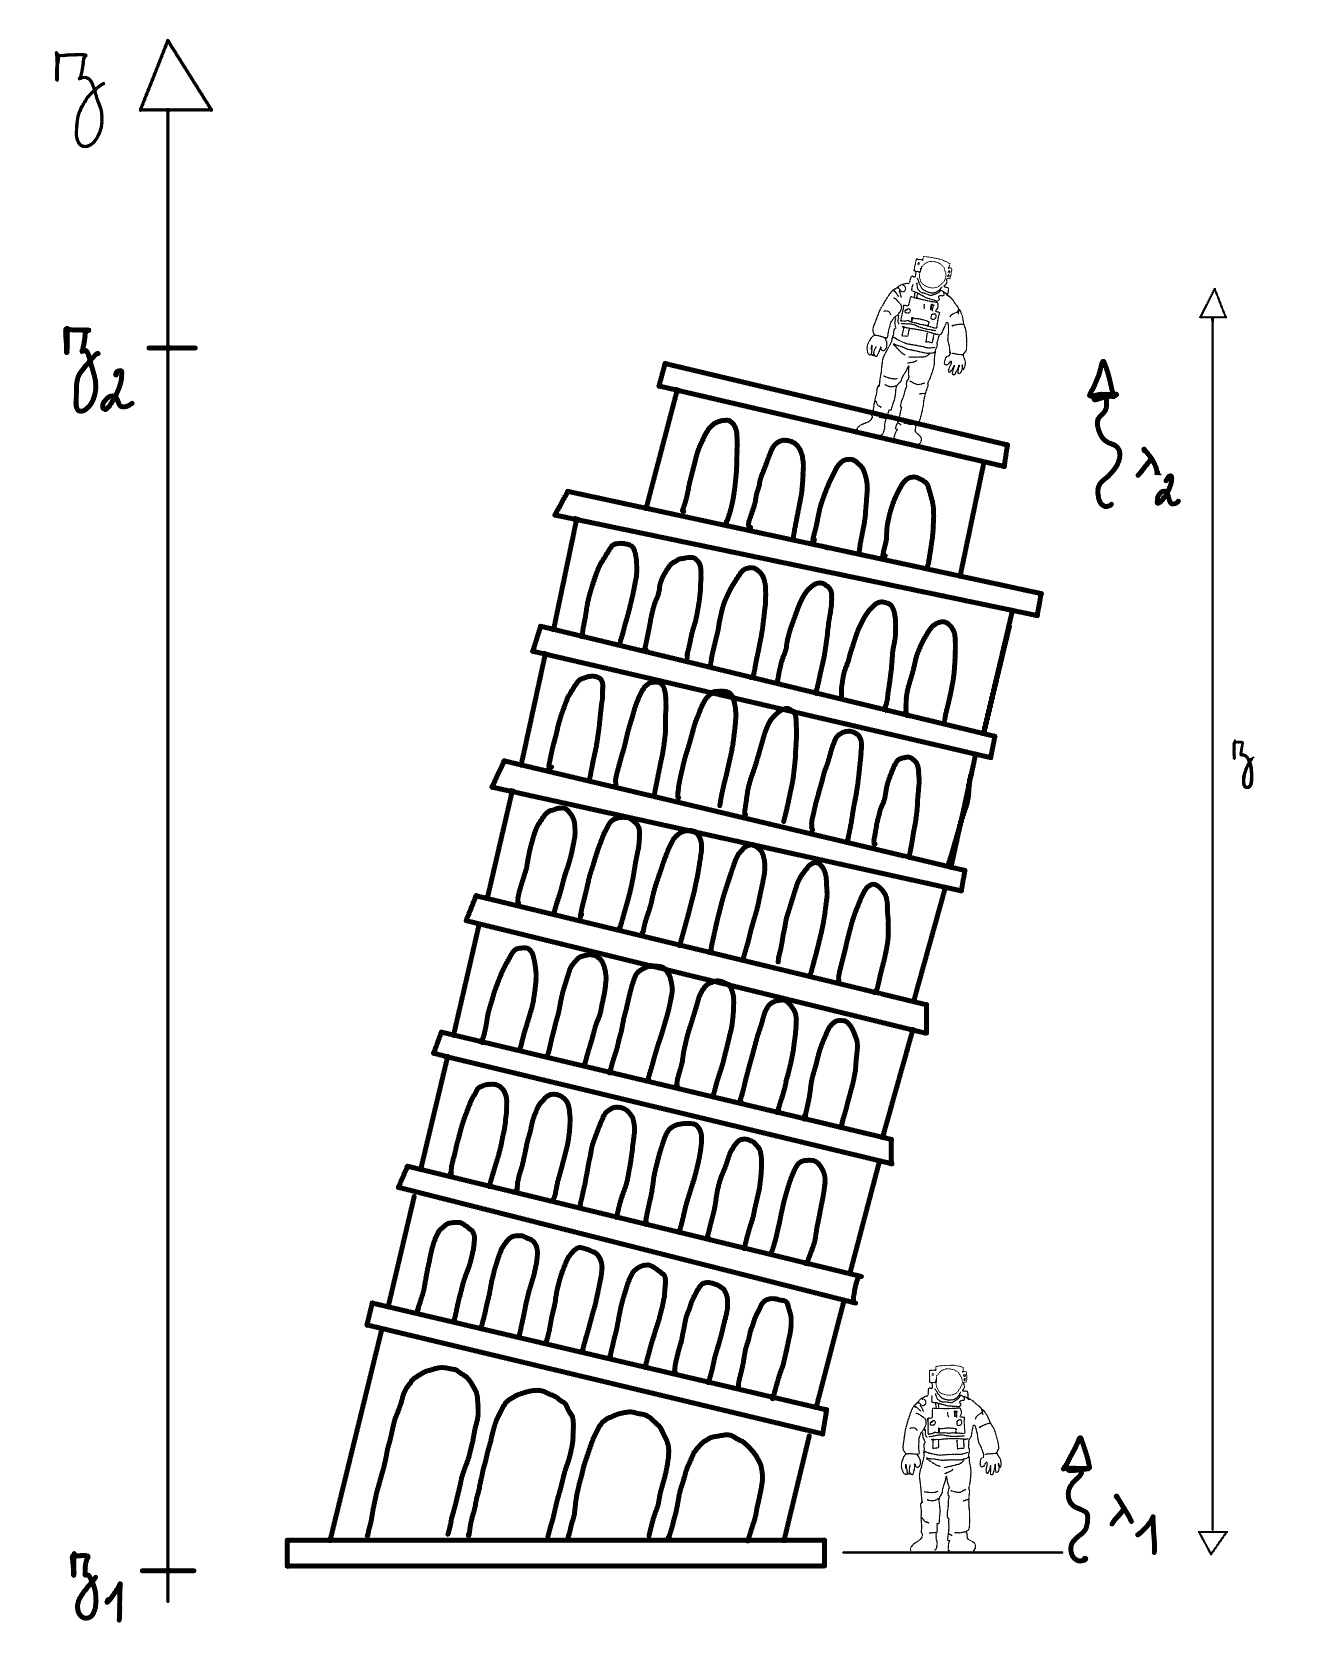
\includegraphics[scale=0.15]{Chapitres/5. Géodésiques/Images/tour de pise.jpg} 
\end{center}

On considère que le champ gravitationnel est statique (indépendant du temps). Les trajectoires $AB$ et $CD$ sont parallèles (cf. ci-dessous). Donc $\td t_{E} = \td t_{R}$. Ceci nous avait troublé parce qu'en espace temps plat, $\td t_{E} = \td t_{R}$ implique que $T_E = T_R \Leftrightarrow \lambda_E \Leftrightarrow \lambda_R$. Or le principe d'équivalence prédit un redshift, qui de plus a été mesuré. Nous allons voir pourquoi il n'y a pas de contradiction. La résolution se trouve dans le fait qu'en présence de gravitation (faible), la métrique n'est plus plate mais décrite par $g_{00} = -\left(1 + \frac{2\Phi}{c^2}\right)$.

\begin{center} 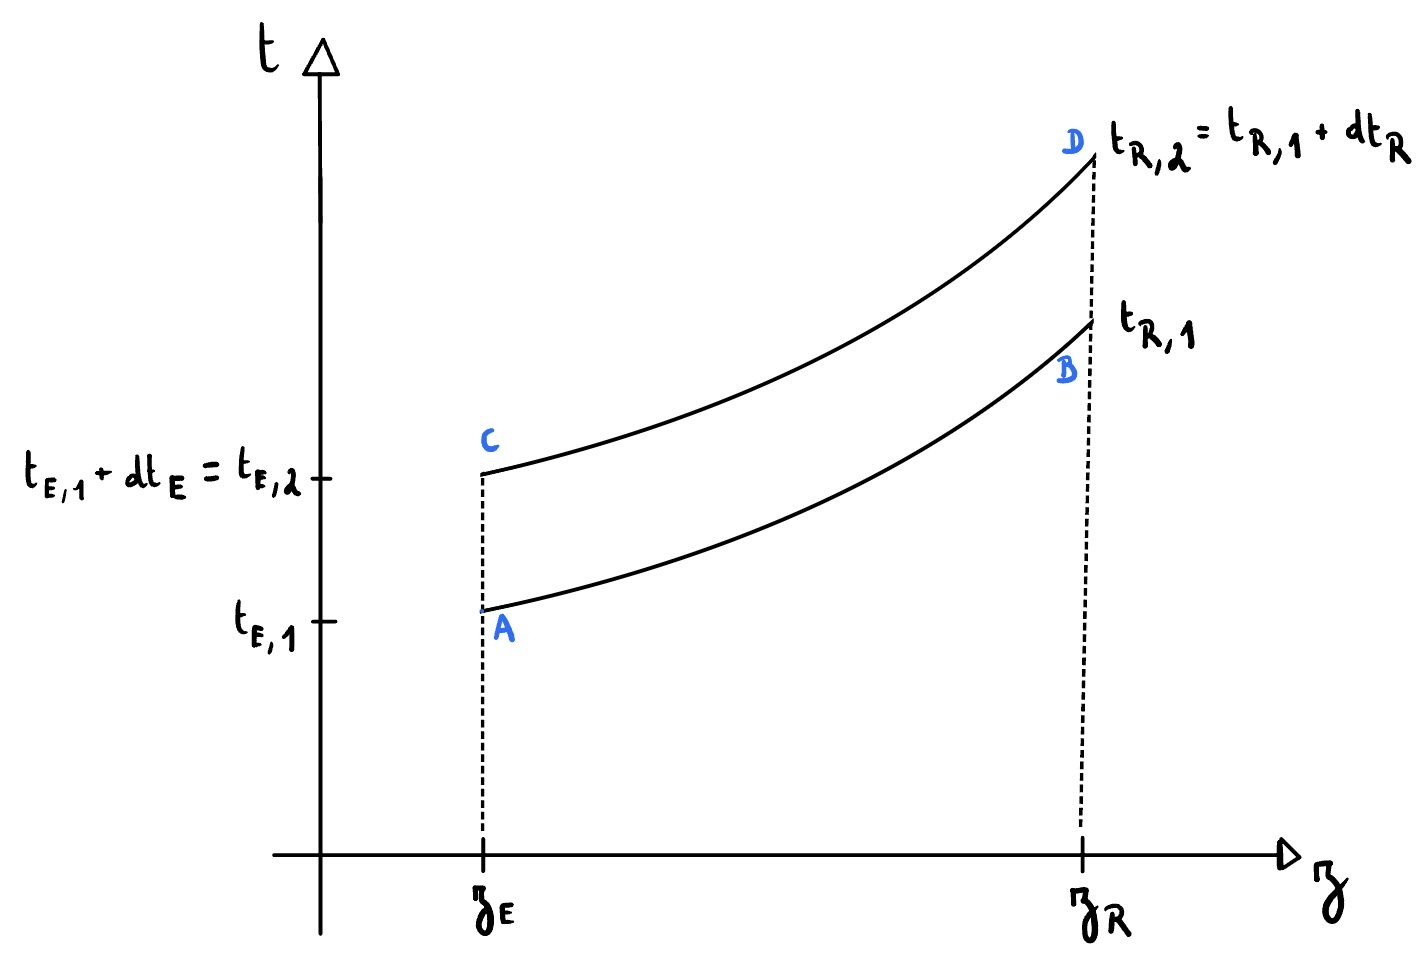
\includegraphics[scale=0.15]{Chapitres/5. Géodésiques/Images/redshift.jpg}  
\end{center}

Le rapport des longueurs d'ondes est donné par 

\begin{equation}
    \frac{\Delta \lambda}{\lambda} = \frac{\lambda -\lambda_0}{\lambda} = \frac{gz}{c^2}=\frac{\Delta \Phi}{c^2}
\end{equation}
où $\vect{g} = -\frac{GM}{r^2}.\vect{1_{r}}$, $\Phi = \frac{GM}{r}$, $\lambda > \lambda_0$, $t_{E, 1}$ est le temps d'émission de la première onde et $t_{E, 2}$ est le temps d'émission de la deuxième onde. 

Le temps propre à l'endroit de l'émission est 
\begin{align}
    \td \tau_E^2 &= -g_{\mu \nu}|_{z_E}\td x^{\mu}\td x^{\nu}\\
    &= - g_{0 0}(z_E)\td t^2_E
\end{align}
Et le temps propre à l'endroit de la réception est 
\begin{align}
    \td \tau_E^2 = - g_{0 0}(z_R)\td t^2_R
\end{align}
Donc même si les intervalles $\td t_E$, $\td t_R$ sont les mêmes (champ statique), les temps propres ne sont pas les mêmes. C'est ces temps propres que les observateurs ont mesuré. 

\begin{equation}
    \frac{\td \tau_E}{\td \tau_R} = \sqrt{\frac{g_{00}(z_E)}{g_{00}(z_R)}}
\end{equation}
car $\td t^2_E = \td t^2_R$. En remplaçant par l'expression de la métrique :


\begin{equation}
     \frac{\td \tau_E}{\td \tau_R} = \sqrt{\frac{1+\frac{2\Phi(z_E)}{c^2}}{1+\frac{2\Phi(z_R)}{c^2}}}
\end{equation}
Comme on suppose que le champ gravitationnel est faible, $\frac{2\Phi(z_E)}{c^2} << 1$, qu'on peut donc développer au premier ordre 

\begin{align}
     \frac{\td \tau_E}{\td \tau_R} = \frac{T_E}{T_R} = \frac{\lambda_E}{\lambda_R} &\simeq \lt 1 +\frac{\Phi(z_E)}{c^2}\rt \lt 1-\frac{\Phi(z_R)}{c^2} \rt\\
     & \simeq 1 - \frac{\Delta \Phi}{c^2}
\end{align}

où $\Delta\Phi = \Phi(z_R) - \Phi(z_E)$. On obtient donc un redshift

\begin{align}
    \frac{\Delta \lambda}{\lambda_R} = 1 - \frac{\lambda_E}{\lambda_R} &= \frac{\Delta\Phi}{c^2}  \\
    &= \frac{GM}{c^2}\lt\frac{1}{R} -\frac{1}{R+z}\rt\\
    &= \frac{GM}{c^2}\lt \frac{R + z - R}{R(R+z)}\rt\\
    & \Delta \frac{GM}{c^2 R^2}z\\
    &=\frac{gz}{c^2}
\end{align}
Donc on trouve que 
\begin{equation}
    \frac{\nabla \lambda}{\lambda} = \frac{gz}{c^2}
\end{equation}
Qui est exactement ce qu'on avait précédemment. Donc la métrique courbe peut expliquer les effets non triviaux dans un champ de gravitation. La métrique courbe explique donc le redshift gravitationnel. 

\section{Déviation des géodésiques et tenseur de Riemann}

Le principe d'équivalence nous a appris que localement les effets d'un champ de gravitation peuvent être annulés en se plaçant dans des coordonnées localement inertielles, qui correspond au référentiel d'un observateur en \emph{chute libre}. Ceci s'était traduit mathématiquement par le fait d'avoir non-seulement $g_{\mu \nu} = \eta_{\mu \nu}$ et $\partial_{\alpha}g_{\mu \nu} = 0 = \Gamma^{\alpha}_{\beta \gamma}$ en un point, mais aussi le long de toute géodésique de genre temps pour des coordonnées bien choisies. Par conséquent, pour détecter la présence d'un champ de gravitation, une seule géodésique (un seul observateur) ne suffit pas. Il faut étudier comment les géodésiques voisines se comportent les unes par rapport aux autres. 

Un postulat fondamental de la géométrie euclidienne, c'est-à-dire de l'espace-temps plat, est que les droites (c'est-à-dire des géodésiques de cet espace) initialement parallèles le restent. En espace-temps courbe c'est-à-dire en présence de gravitation, deux droites peuvent s'intercepter. Cet effet est facilement illustré sur la sphère. Des géodésiques initialement parallèle sur une sphère vont finir par s'intercepter. 

\begin{center} 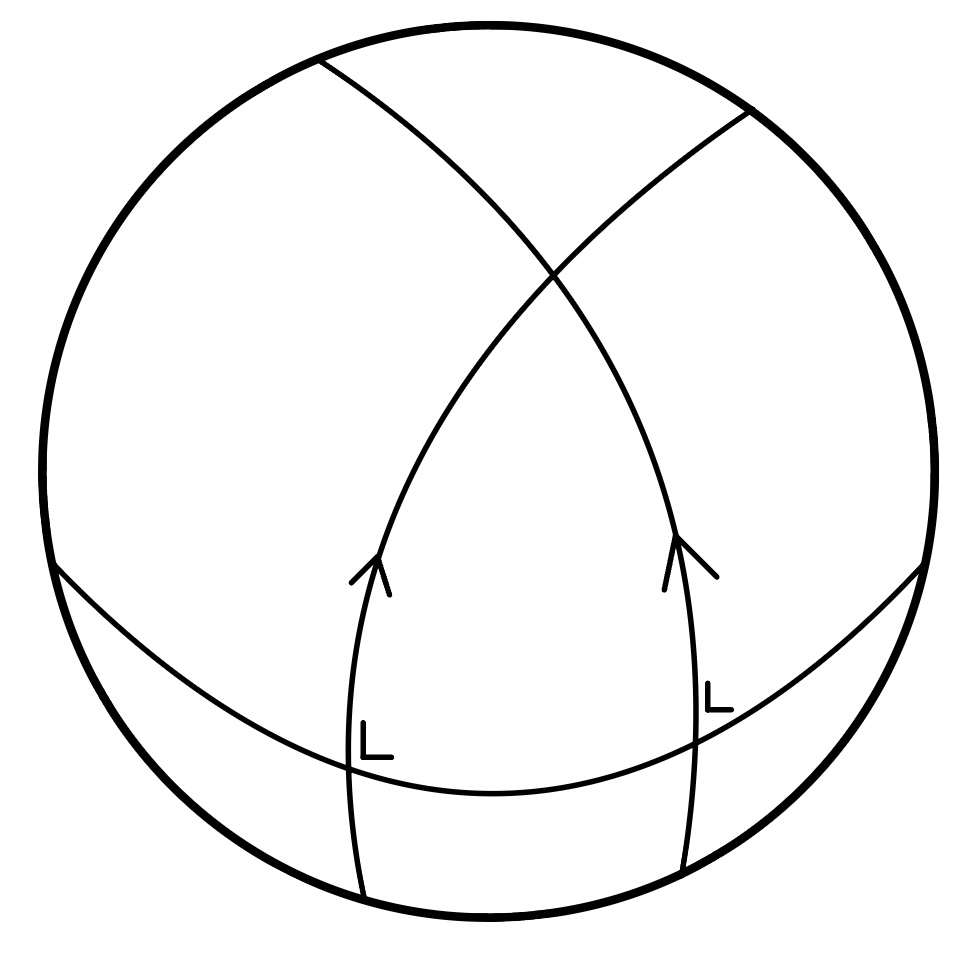
\includegraphics[scale=0.15]{Chapitres/5. Géodésiques/Images/sphere trajectoire qui se croise.jpg} 
\end{center}

\subsection{Le cas Newtonien}
On voudrait quantifier ce comportement dans un espace-temps courbe. Pour ce faire, on va d'abord étudier ce comportement dans un champ Newtonien. 

Une particule se déplaçant dans un champ de gravitation suit la trajectoire suivante :

\begin{equation}
    \frac{\td^2x^{i}}{\td t^2} = -\partial^{i}\Phi(x)
\end{equation}

Considérons à présent 2 particules voisines l'une en $x^{i}(t)$ et l'autre en $x^{i}(t) + \delta x^{i}(t)$. 

\begin{center} 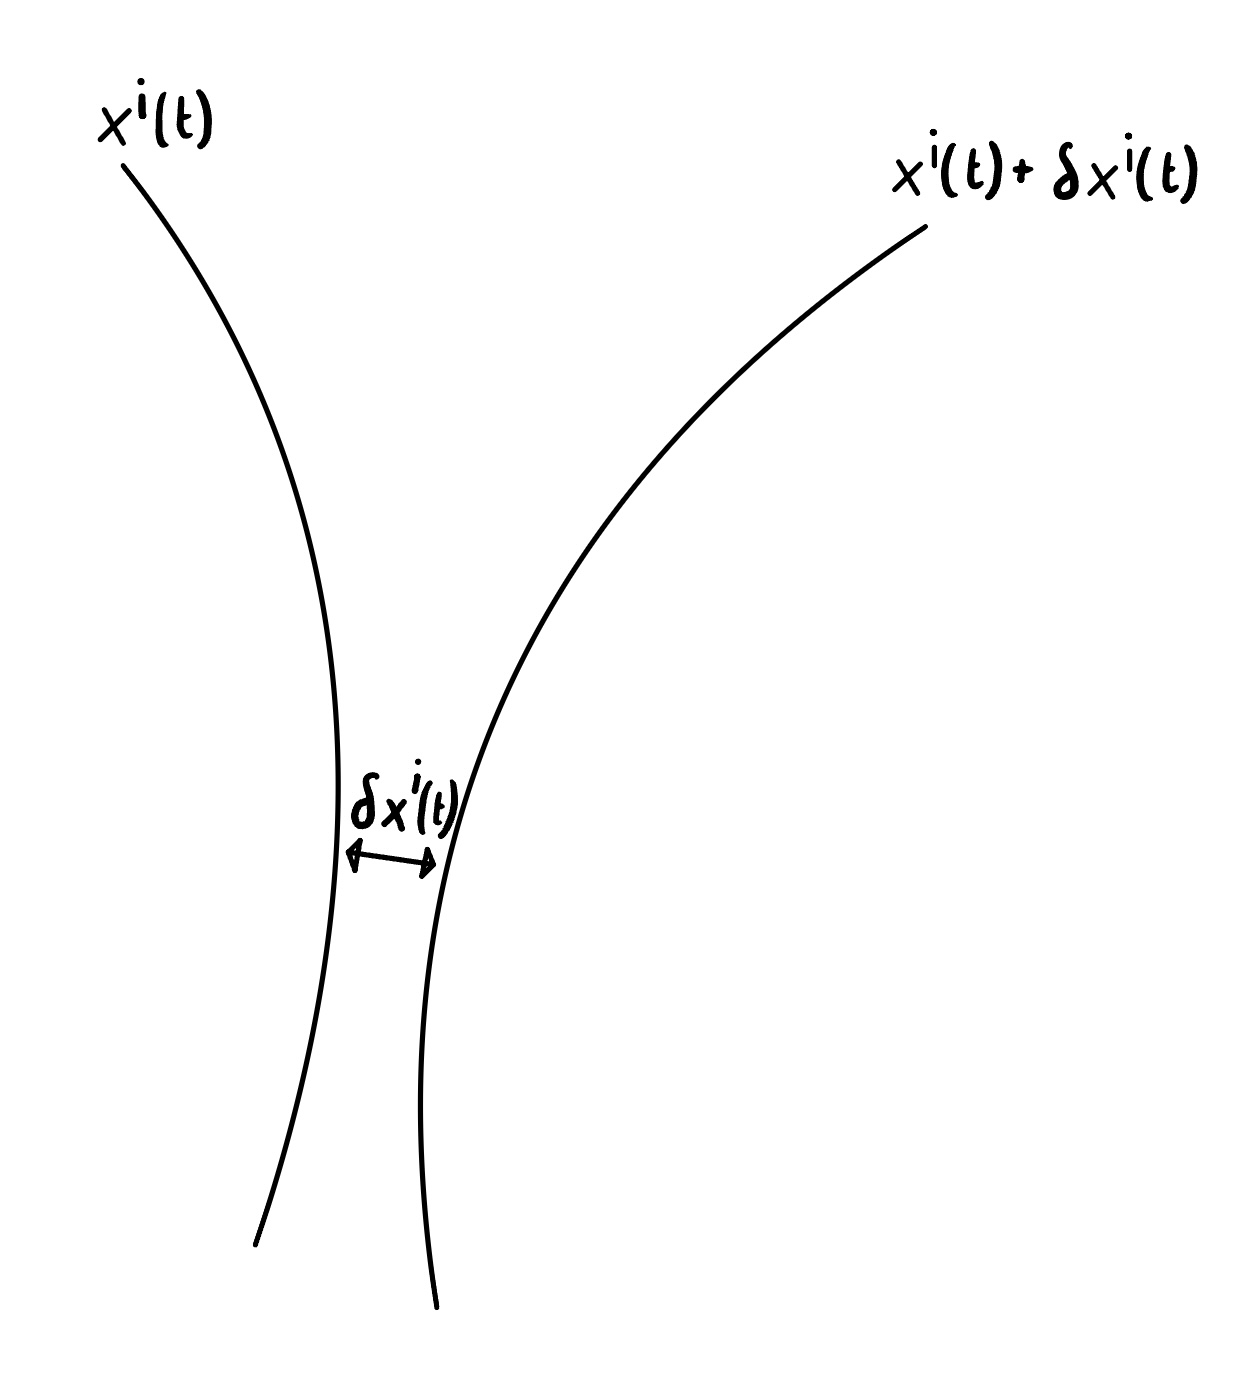
\includegraphics[scale=0.15]{Chapitres/5. Géodésiques/Images/mouvement infinitésimal.jpg} 
\end{center}

La deuxième particule obéit à l'équation suivante:

\begin{equation}
    \frac{\td ^2}{\td t^2}(x^{i}(t) + \delta x^{i}(t)) = -\partial^{i}\Phi(x + \delta x)
\end{equation}
On sait que 

\begin{equation}
    \frac{\td ^2}{\td t^2}(x^{i}(t) + \delta x^{i}(t))= \frac{\td ^2}{\td t^2}(x^{i}(t) ) + \frac{\td ^2}{\td t^2}(\delta x^{i}(t))
\end{equation}
Et on a aussi que

\begin{equation}
    \pd^i \Phi(x+\delta x) = \partial^{i}\Phi(x) + \partial_{j}(\partial^{i}\Phi(x))\delta x^{j}+\mathcal{O}(\delta x^2)
\end{equation}

On obtient donc
\begin{equation}
    \frac{\td ^2}{\td t^2}(\delta x^{i}(t)) = - \partial_{j}(\partial^{i}\Phi(x))\delta x^{j}
    \label{eq:forces de marées gravitationnelles}
\end{equation}
Cette équation décrit l'effet des forces de marées gravitationnelles (le gradient de la force gravitationnelle) sur une famille de 
particules se déplaçant dans un champ de gravitation.

\begin{center} 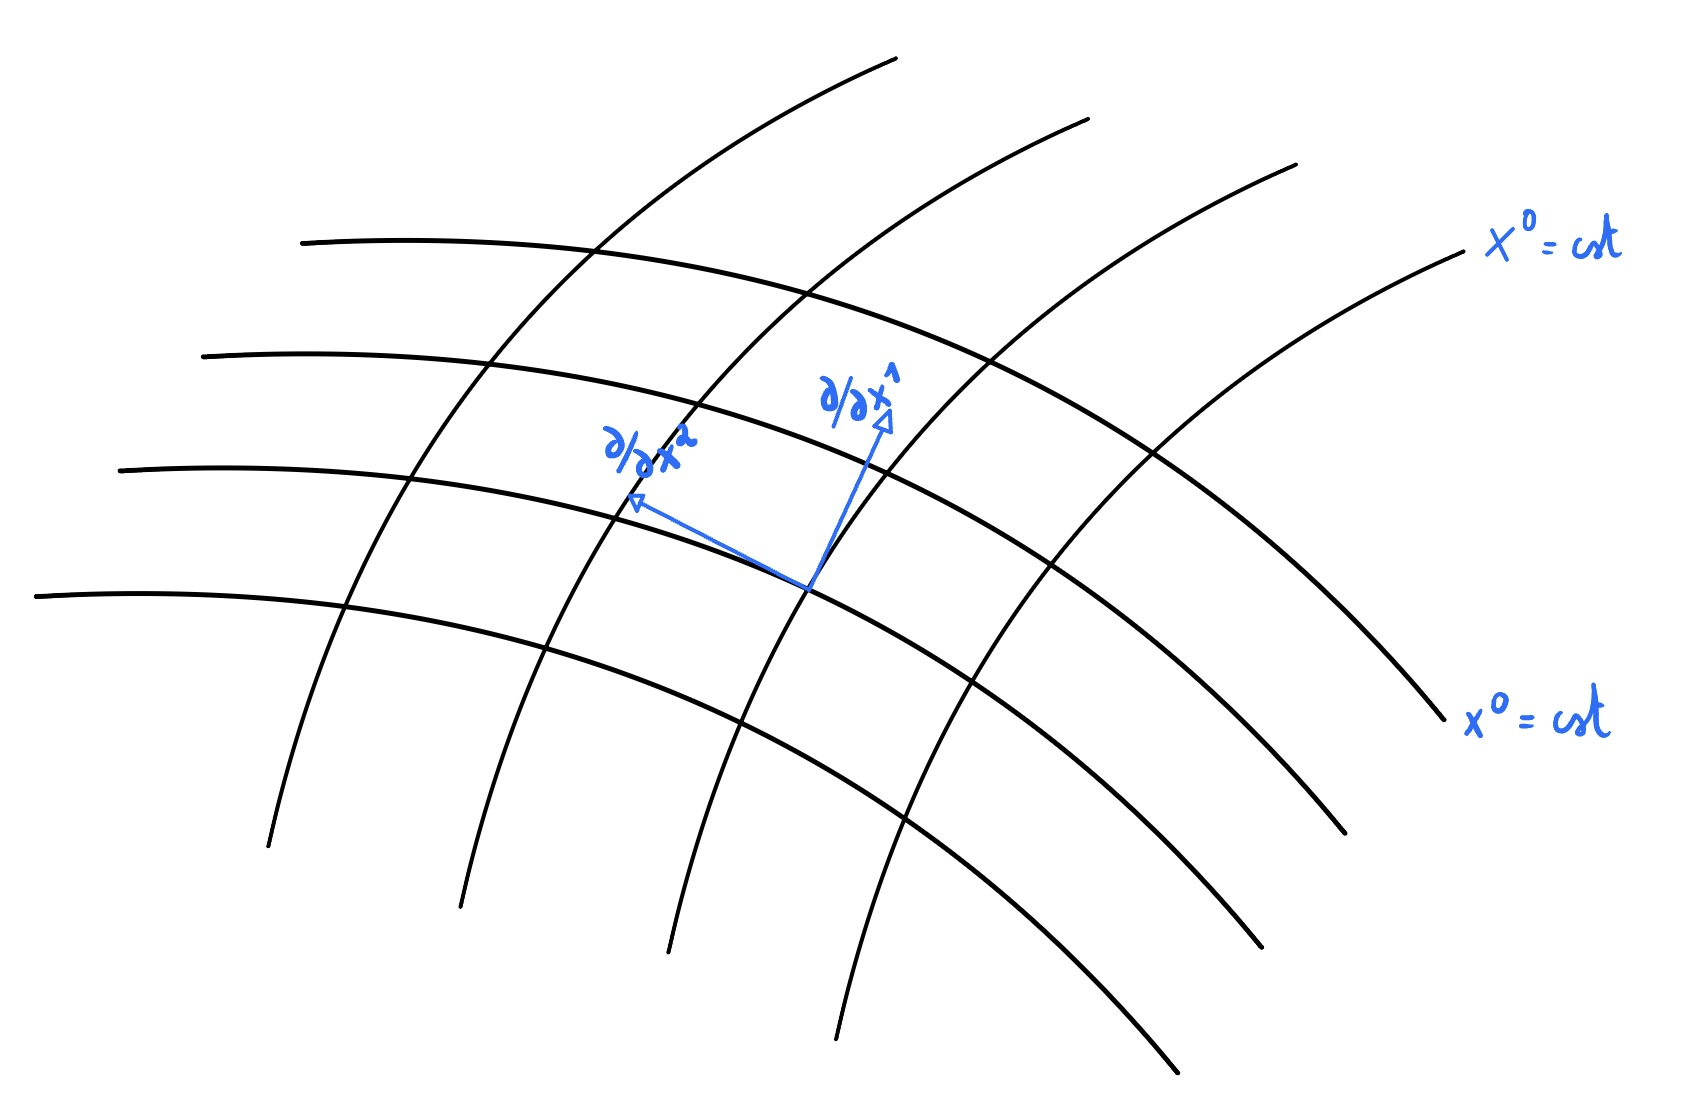
\includegraphics[scale=0.15]{Chapitres/5. Géodésiques/Images/courbure d'espace .jpg} 
\end{center}

\subsection{Généralisation covariante}
Considérons à présent un variété arbitraire $(\mathcal{M},g)$ munie de sa connexion de Levi-Civita. Soit une famille de géodésiques $\{\gamma_{s}(t)\}_s$ de paramètre affine $t$. Pour chaque valeur de $s$, on a une géodésique. Soit une carte locale et notons les champs tangents $T = T^{\mu}\partial_{\mu}$ d'une géodésique : 

\begin{equation}
    T^{\mu} = \left. \frac{\td x^{\mu}}{\td t}(\gamma_{s}(t))\right|_{s \text{ fixé}} = \frac{\pd x^{\mu}}{\pd t}(\gamma_{s}(t))
\end{equation}
qui est un champ tangent à la géodésique $s$. Par définition d'une géodésique, il est transporté parallèlement à lui-même:
\begin{equation}
    \nabla_{T}T = 0
\end{equation}
On définit également le \emph{déplacement} $S$ d'une géodésique à une géodésique voisine :
\begin{equation}
    S^{\mu} =\left. \frac{\td x^{\mu}}{\td s}(\gamma_{s}(t))\right|_{t \text{ fixé}}= \frac{\partial x^{\mu}}{\partial s}(\gamma_{s}(t))
\end{equation}
C'est la généralisation covariante de la séparation $\delta x^{i}$ utilisée auparavant. On voudrait calculer comment ce champ de vecteurs évolue lorsqu'on se déplace le long des géodésiques. On définit la vitesse relative des géodésiques par 

\begin{equation}
    V^{\mu} = (\nabla_{T}S)^{\mu} = T^{\rho}\nabla_{\rho}S^{\mu} \equiv \frac{\mathrm{D}}{\td t}S^{\mu}
\end{equation}
où $\frac{\td }{\td t} = T^{\mu}\partial_{\mu} \rightarrow \frac{\mathrm{D} }{\td t} = T^{\mu}\nabla_{\mu}$. L'accélération relative est définie comme :

\begin{equation}
    A^{\mu} = (\nabla_{T}V)^{\mu}\equiv\frac{\mathrm{D} ^2}{\td t^2}S^{\mu}
\end{equation}
Nous souhaiterions calculer $A^\mu$ et nous montrerons que celle-ci est intrinsèque à la courbure et donc à la variété.
Le résultat sera la généralisation covariante de l'équation [\ref{eq:forces de marées gravitationnelles}]. Notons d"jà que lorsque $A^{\mu}=0$, la métrique est plate. 

\subsubsection{Calcul de $A^\mu$}
Notons d'abord que la famille de géodésiques $\gamma_{s}(t)$ balaye une surface bidimensionnelle (à paramètres $(s,t)$) sur la variété $\mathcal{M}$ qui forme une sous variété de dimensions $2$ de $\mathcal{M}$. L'espace tangent de cette sous variété a pour base les vecteurs $S$ et $T$ (en tout point $S$ et $T$ sont linéairement indépendant). C'est-à-dire que les champs de vecteurs $S^{\mu}$ et $T^{\mu}$ définissent localement une base de l'espace tangent à cette sous-variété. Autrement dit, chaque point de cette sous-variété est uniquement décrite par la donnée d'une paire $(s,t)$.
\begin{theoremframe}
    \begin{propri} 
        Le crochet de Lie
        \begin{equation}
            [S,T] = 0
        \end{equation}
        est nul.
    \end{propri}
\end{theoremframe}
\begin{proof}

Rappelons que le crochet de Lie est défini comme
\begin{equation}
[S,T] \equiv S^{\mu}\partial_{\mu}T^{\nu} - T^{\alpha}\partial_{\alpha}S^{\nu}
\end{equation}
Considérons donc que les champs de vecteurs:

$$S = \frac{\partial}{\partial_{s}}$$, $$T = \frac{\partial}{\partial_{t}}$$

sont dans un système de coordonnées où $[S, T] = 0$. Comme le crochet de Lie est un champ de vecteurs (se transforme de manière covariante), si le commutateur est nul dans un système de coordonnée, il est nul dans tout système de coordonnée.
\end{proof}
\begin{theoremframe}
    \begin{propri}
        Pour une connexion sans torsion, on a que 

        \begin{equation}
            [S,T] = S^{\mu}\partial_{\mu}T^{\nu} - T^{\alpha}\partial_{\alpha}S^{\nu} = S^{\mu}\nabla_{\mu}T^{\nu} - T^{\alpha}\nabla_{\alpha}S^{\nu}
        \end{equation}
    \end{propri}
\end{theoremframe}
\begin{proof}
On peut prouver cette égalité de deux manières différentes. Soit on remarque que cette objet est tensoriel et alors on peut évaluer cette égalité dans un système de coordonnées localement inertiel. Dans un telle système de coordonnées on avait vu que $\nabla = \partial$. 

Sinon, on peut également calculer explicitement $S^{\mu}\nabla_{\mu}T^{\nu} - T^{\alpha}\nabla_{\alpha}S^{\nu}$. En développent, les termes en $\Gamma$ vont s'annuler pour une connexion sans torsion et il restera uniquement les termes avec les dérivées partielles, ce qui prouve l'identité.
\end{proof}
Ces deux propriétés impliquent

\begin{equation}
    S^{\mu}\nabla_{\mu}T^{\nu} - T^{\alpha}\nabla_{\alpha}S^{\nu} = 0
    \label{eq:champ de vecteur S et T}
\end{equation}
L'accelération s'écrit alors
\begin{align}
    A^{\mu} &= T^{\rho}\nabla_{\rho}(T^{\sigma}\nabla_{\sigma}S^{\mu})\\
    \intertext{Par l'équation \ref{eq:champ de vecteur S et T} :}
    &= T^{\rho}\nabla_{\rho}(S^{\sigma}\nabla_{\sigma}T^{\mu})\\
    \intertext{Par la règle de Leibniz}
    &= \textcolor{purple}{T^{\rho}\nabla_{\rho}S^{\sigma}} \nabla_{\sigma}T^{\mu} + T^{\rho}S^{\sigma}(\textcolor{blue}{\nabla_{\rho}\nabla_{\sigma}}T^{\mu})\\
    &= \textcolor{purple}{S^\rho \nabla_\rho T^\sigma} \nabla_\sigma T^\mu +T^{\rho}S^{\sigma}(\textcolor{blue}{[\nabla_{\rho},\nabla_{\sigma}]}T^{\mu}) +T^{\rho}S^{\sigma}(\textcolor{blue}{\nabla_{\sigma}\nabla_{\rho}}T^{\mu}) 
    \intertext{Or, comme $[\nabla_{\rho}, \nabla_{\sigma}]T^{\mu} = R^{\mu}_{\alpha \rho \sigma}T^{\alpha}$ :}
    &= S^{\rho}\nabla_{\rho}T^{\sigma}\nabla_{\sigma}T^{\mu}+ T^{\rho}S^{\sigma}\nabla_{\sigma}\nabla_{\rho}T^{\mu} + T^{\rho}S^{\sigma}R\indices{^{\mu}_{\alpha \rho \sigma}} T^{\alpha}
\end{align}
Une intégration par parties donne alors 
\begin{align}
    T^{\rho}S^{\sigma}\nabla_{\sigma}\nabla_{\rho}T^{\mu} = S^{\sigma}\nabla_{\sigma}(T^{\rho}\nabla_{\rho}T^{\mu}) - S^{\sigma}\nabla_{\sigma}T^{\rho}\nabla_{\rho}T^{\mu}
\end{align}
Or, $S^{\sigma}\nabla_{\sigma}(T^{\rho}\nabla_{\rho}T^{\mu}) = \nabla_S \nabla_T T^\mu 0$ (pour une géodésique $\nabla_{T} T=0$). On réécrit alors
\begin{align}
     A^{\mu} &=S^{\rho}\nabla_{\rho}T^{\sigma}\nabla_{\sigma}T^{\mu}- S^{\sigma}\nabla_{\sigma}T^{\rho}\nabla_{\rho}T^{\mu}+ T^{\rho}S^{\sigma}R\indices{^{\mu}_{\alpha \rho \sigma}}T^{\alpha}\\
     &=T^{\rho}S^{\sigma}R\indices{^{\mu}_{\alpha \rho \sigma}} T^{\alpha}
\end{align}
Finalement, on obtient que 

\begin{equation}
    \boxed{A^{\mu} = T^{\rho}S^{\sigma}R\indices{^{\mu}_{\alpha \rho \sigma}}T^{\alpha}}
\end{equation}
Cette équation est appelé équation de déviation géodésique (ou équation de Jacobi). 
On remarque que l'accélération relative est complètement capturée par le tenseur de Riemann, qui est une quantité intrinsèque à la variété\footnote{Peut être définie sans nécessiter un espace ambiant dans lequel est plongée la variété (comme p.ex. une surface $S \subset \R^3$). En effet, la métrique elle-même peut être définie de manière intrinsèque, et le tenseur de Riemann pour une connexion de Levi-Civita est uniquement déterminée à partir de la métrique.} et qui caractérise la courbure de celle-ci. Le tenseur de Riemann est donc responsable de l'accélération relative de 2 géodésiques voisines. 
\begin{exmp}
    Dans un espace plat, $R^{\mu}_{\alpha \rho \sigma} = 0$ et donc $A^{\mu} =0$. Ainsi :
    \begin{equation}
        S^{\mu} = \delta x^{\mu}(t) = C^{\mu}t + D^{\mu}
    \end{equation}
où $C$ et $D$ sont des constantes. Ainsi $S^{\mu}$ est une fonction linéaire du temps. On retrouve les axiomes d'Euclide qui dit que 2 lignes droites s'intersectent au plus une fois et que 2 droites parallèles ne peuvent pas s'intersecter.
\end{exmp}


\chapter{Les équations d'Einstein}
Mentionnons à nouveau la citation de \emph{Wheeler} :
\begin{center}
    \emph{Matter tells space-time how to bend, space-time tells matter how to move.}
\end{center}
Dans le chapitre précédent, nous avons étudié comment des \emph{particules-test} se déplacent dans un champ gravitationnel (manifesté par une métrique non-triviale et régi par l'équation des géodésiques). Étant donné une métrique, nous pouvons donc calculer la trajectoires de particules soumis à la force gravitationnelle résultante de cette métrique. Au chapitre présent, nous nous intéresserons à la première partie de la citation de \emph{Wheeler} : quelle est la forme de la métrique pour une distribution d'énergie (de masse) donnée.\footnote{Il s'agit de l'analogue gravitationnel des équations de Maxwell, alors que l'équation des géodésiques était l'analogue de la force de Lorentz.}\\
\\
Le principe fondamental de la relativité générale est que l'interaction gravitationnelle se manifeste par la courbure de l'espace-temps et que les corps soumis uniquement au champ gravitationnel (dits "en chute libre") suivent des géodésiques de cet espace-temps courbe. Ainsi, l’interaction gravitationnelle n'est pas vue comme une force, mais plutôt comme l'effet de la courbure de l'espace-temps. Dans le chapitre précédent, on a retrouvé les équations du mouvement Newtoniennes d'un champ de gravitation à partir de l'équation des géodésiques pour une métrique telle que $g_{00} = -\left(1 + \frac{2\Phi}{c^2}\right)$ dans la limite Newtonienne :

\begin{equation}
    \frac{\td^2x^{i}}{\td t^2} = -\partial^i \Phi
\end{equation}

où $\Phi = -\frac{GM}{r} $ pour un champ dû à une particule à masse ponctuelle $M$, avec la constante gravitationnelle $G = 6,67.10^{-11} \frac{\text{m}^3}{\text{kg} \text{ s}^2}$. 

Nous allons exposer deux méthodes pour dériver les équations d'Einstein : 
\begin{enumerate}
    \item L'approche historique "\emph{heuristique}" suivie par Einstein.
    \item Une dérivation par un principe variationnel.
\end{enumerate}
Nous souhaitons imposer que dans la limite des champs faibles, ces équations se réduisent à l'équation du potentiel gravitationnel de la théorie de Newton (l'équation de Poisson) :
\begin{equation}
    \Delta \Phi = 4\pi G\rho
    \label{eq:Poisson}
\end{equation}
où $\rho$ est la densité de masse. C'est ce que nous montrerons dans la première approche. Nous allons ensuite montrer que ces mêmes équations dérivent également d'un principe variationnel.

Pour généraliser l'équation de Poisson, nous aimerions réécrire cette équation sous forme tensorielle. Pour le membre de gauche de l'équation de Poisson, on a vu en étudiant les géodésiques et leur limite newtonienne que le rôle du potentiel gravitationnel $\Phi$ devrait être joué par la métrique (via le principe d'équivalence). On s'attend donc à ce qu'une généralisation covariante de $\Delta \Phi$ impliquera des dérivées seconde de la métrique. L'objet tensoriel le plus simple faisant intervenir les dérivées secondes de la métrique est de la forme
\begin{equation}
    \nabla_{\alpha}\nabla_{\beta}g_{\mu \nu}
\end{equation}
mais celui-ci est automatiquement nul partout en considérant notre choix de connexion. Néanmoins, nous avions vu qu'il existait d'autres quantités tensorielles construites à partir des dérivées secondes de la métriques comme le tenseurs de Riemann, le tenseur de Ricci et la courbure scalaire. 

Mais avant de nous intéresser à la généralisation du membre de gauche, penchons-nous sur le membre de droite, i.e. à la généralisation de la densité de masse.

\section{Le tenseur d'énergie-impulsion en relativité restreinte}

\subsection{Rappel: le quadrivecteur impulsion}

Considérons une particule massive de masse $m$, suivant donc une trajectoire de genre temps $x^{\mu}(\tau)$, où on a choisi une paramétrisation par le temps propre qui, pour rappel, est défini selon

\begin{equation}
    \td \tau ^2 = -\td s^2 = -g_{\mu \nu}\td x^{\mu}\td x^{\nu}
\end{equation}
\begin{theoremframe}
    \begin{defi}
        Le quadrivecteur vitesse de la particule est le vecteur tangent à la trajectoire dans la paramétrisation avec le temps propre. Celui-ci est donc donné par
        \begin{equation}
            U^{\alpha} = \frac{\td x^{\mu}}{\td \tau}
        \end{equation}
        qui vérifie la relation de normalisation $U^{\alpha}U_{\alpha} = -1$
    \end{defi}
\end{theoremframe}

\begin{theoremframe}
    \begin{defi}
        Le quadrivecteur impulsion de la particule est défini comme
        \begin{equation}
            P^{\mu} = mU^{\mu} = (\frac{E}{c^2}, \vect{P})
        \end{equation}
        où nous avons temporairement réintroduit la constante $c$.
        \end{defi}
\end{theoremframe}
L’énergie de la particule est la première composante du quadrivecteur impulsion :
\begin{equation}
    E \equiv P^{0} c^2
\end{equation}
En tant que composante d'un quadrivecteur, l'énergie n'est pas une quantité scalaire, mais dépend de l'observateur, car la loi de transformation mélange l'énergie avec les autres composantes du vecteur. Autrement dit, l'énergie n'est pas une quantité invariante sous changement général de coordonnées. 
\begin{exmp}
    Dans les coordonnées d'un observateur $O$ au repos par rapport à la particule (observateur co-mobile), le vecteur tangent de la trajectoire de la particule est donné par
    \begin{equation}
        U^{\mu} = (1,0,0,0)
    \end{equation}
    et donc l'impulsion est $P^{\mu} = (m,0,0,0)$. L'énergie vaut alors
    \begin{align}
        &P^0 = \frac{E}{c^2}=m\\
        \implies &E = mc^2
    \end{align}
    L'expression $E = mc^2$ est l'énergie au repos de la particule. Néanmoins, dans un autre référentiel $O'$ se déplaçant à une vitesse $v$ dans la direction $x$ par rapport au référentiel $O$ n'observera pas la même énergie. En effet, la transformation de Lorentz s'écrit :
    \begin{equation}
        \left\{
        \begin{array}{l}
            t' = \gamma (t + vx)\\
            x' = \gamma (x + vt)
        \end{array}
        \right.
    \end{equation}
    L'impulsion mesurée dans le référentiel $O'$ est alors obtenu via 
    \begin{equation}
        P'^{\alpha} = \frac{\partial x'^{\alpha}}{\partial x^{\beta}} P^{\beta}
    \end{equation}
    L'énergie est alors donnée par
    \begin{equation}
        E' = P'^{0}c^2 = \frac{\partial x'^{0}}{\partial x^{0}} P^{0}c^2 = \frac{\partial x'^{0}}{\partial x^{0}}m c^2= \gamma m c^2
    \end{equation}
    Lorsque $v\ll c$, nous pouvons développer le facteur de Lorentz en premier ordre :
    \begin{align}    
        E = mc^2 + \frac{1}{2}mv^2 + \mathcal{O}\left(\frac{v}{c}\right)^2
    \end{align}
    où le premier terme correspond à l'énergie au repos et le second terme à l'énergie cinétique. 
\end{exmp}
\subsection{Le tenseur d'énergie-impulsion mésoscopique}
Bien que le (quadrivecteur) impulsion contient toute l'information nécessaire à la description de l'énergie et de l'impulsion d'une particule individuelle, il n'est pas approprié pour décrire des systèmes étendus constitués d'un grand nombre de particules. Dans ce cas, plutôt que de spécifier les impulsions individuelles de chaque particule, on préférera de décrire le système à une échelle mésoscopique, comme un fluide (c'est-à-dire comme une distribution continue caractérisé par des quantités macroscopique comme la densité, la pression, l'entropie, la viscosité, etc...). Le comportement de ce fluide ne dépend que des propriétés moyennes d'une grande collection de particules et pas des propriétés individuelles. Ces propriétés moyennes peuvent varier d'un point à l'autre du fluide. En pratique cela revient à sous-diviser le système en "élément de fluide" suffisamment grands pour que les propriétés individuelles des particules ne jouent pas, mais assez petits que pour pouvoir capturer le comportement local du fluide (l'échelle \emph{mésoscopique}). 

L'objet qui capture les propriétés d'un fluide (au sein duquel règne un champ $P^{\mu}$ de quadrivecteurs impulsion) est le tenseur énergie-impulsion.
\begin{theoremframe}
    \begin{defi}
        Le tenseur énergie-impulsion est un tenseur $(0,2)$ tel que $T^{\mu \nu} $ est le flux d'impulsion $P^{\mu}$ à travers la surface $x^{\nu} = \text{cste}$.
    \end{defi}
\end{theoremframe}
C'est un tenseur symétrique qui contient toute l'information sur l'énergie d'un système. Par convention, ses unités sont fixés à $[T^{\mu\nu}] = E/L^3$.
\subsection{Interprétation des composantes du tenseur $T^{\mu\nu}$}
Interpréter de cette définition n'est, à première vue, pas évident : qu'entend-on par flux à travers la surface $t = \text{cste}$ ? \\
Rappelons d'abord la définition du flux à travers la surface $\mathcal{S}=\{x=\text{cste}\}$. Celui-ci est défini comme le nombre de particules (i.e. lignes d'Univers) qui traversent cette surface $\mathcal{S}$ par unité de temps. Mais nous avons deux dimensions($y$ et $z$) en plus. Si on veut calculer le flux en un point, il faut s'intéresser à un cube unité $\Delta t= \Delta y = \Delta z = 1$ et à $x$ fixé.
\begin{theoremframe}
    \begin{defi}
        Le flux à travers $x=\text{ cste}$ est le nombre de particules (ou lignes d'Univers) qui traversent $\mathcal{S}$ par unité de temps et par unité de surface transverse. 
    \end{defi}
\end{theoremframe}
Ceci nous permet d'apporter une interprétation similaire au flux à travers  $t=\text{ cste}$: il faut mesurer le nombre de particules qui se trouvent dans le cube unité $\Delta x= \Delta y = \Delta z = 1$ et à $t$ fixé. Ceci est le flux temporel par unité de volume : il s'agit d'une densité.

\begin{theoremframe}
    \begin{defi}
        Le flux à travers $t=\text{ cste}$ ou flux temporel correspond à une densité spatiale. 
    \end{defi}
\end{theoremframe}
En particularisant pour le flux de $P^0$, on trouve immédiatement
\begin{theoremframe}
    \begin{propri}
        La composante $T^{00}$ est une densité d'énergie :
        \begin{equation}
            T^{00}= \rho c^2
        \end{equation}
    \end{propri}
\end{theoremframe}
Similairement, pour $P^i$, on trouve \\
\\
\begin{theoremframe}
    \begin{propri}
        Le tenseur $T^{0i} $ est le flux d'énergie à travers $x^{i}=\text{ cste}$ :
        \begin{equation}
            T^{0i} =\frac{1}{c} \times (\text{Flux d'énergie à travers } \; \mathcal{S}) = \frac{1}{c} \rho c^2 v^i = \rho c v^i
        \end{equation}
    \end{propri}
\end{theoremframe}
où le facteur $1/c$ est imposé par notre choix d'unités.
\begin{theoremframe}
    \begin{defi}
        Le tenseur $T^{i0}$ est une densité d'impulsion $P^{i}$ :
        \begin{equation}
            T^{i0} = c \frac{m v^i}{V} = \rho v^i c
        \end{equation}
    \end{defi}
\end{theoremframe}
où à nouveau, le facteur $c$ apparaît par notre choix d'unités. On remarque donc qu'on a bien $T^{i0} = T^{0i}$.

\begin{theoremframe}
    \begin{defi}
    L'objet $T^{ij}$, appelé tenseur des torsions, représente les forces entre des éléments infinitésimaux de fluide voisins.
    \begin{equation}
        T^{ij} = \rho v^i v^j
    \end{equation}
    \end{defi}
\end{theoremframe}
En considérant deux volumes de fluides infinitésimaux voisins séparés par la surface $z = \text{cste}$, la force de pression exercée par $A$ sur $B$ est $\vect{F} = \frac{\td\vect{P}}{\td t}$. Le flux d'impulsion à travers $z = \text{cste}$ est $\frac{\vect{F}}{\mathcal{S}}$ où $\mathcal{S}$ est une surface séparant $A$ et $B$. Ainsi, $\frac{\vect{F}^{i}}{\mathcal{S}}$ correspond au flux de la composante $P^{i}$ à travers $z = \text{cste}$.

Or, comme la composante $x^{i}$ du flux à travers $z = \text{cste}$ pour l'élément $A$ est 

\begin{equation}
    T^{iz} = \frac{\vect{F}^{i}}{\mathcal{S}}
\end{equation}

\begin{theoremframe}
    \begin{defi}
        Les composantes $T^{xz}$ et $T^{yz}$ mesurent le frottement (viscosité) entre éléments fluides, c'est-à-dire qu'ils mesurent les forces de cisaillement. 

        La composante $T^{zz}$ mesure la pression selon $z$. 
    \end{defi}
\end{theoremframe}
\begin{theoremframe}
    \begin{propri}
        Le tenseur des torsion est symétrique : $T^{ij} = T^{ji}$.
    \end{propri}
\end{theoremframe}
\begin{proof}
    Exercice.
\end{proof}
\begin{rmk}
    La description ci-dessus est une description phénoménologique. Dans certains cas, on dispose d'une description microscopique de la matière en question, sous la forme d'un Lagrangien (champ scalaire, électromagnétique, modèle standard, ...). Il eciste une procédure canonique pour construire le tenseur d'énergie-impulsion à partir du théorème de Noether.
\end{rmk}
\begin{theoremframe}
    \begin{propri}
        Le tenseur d'énergie-impulsion est \emph{conservé} :
        \begin{equation}
            \pd_\mu T^{\mu\nu} = 0
        \end{equation}
        pour un fluide dans un référentiel inertiel soumis à aucune force extérieure (c'est-à-dire que $T^{\mu \nu}$ comprend toutes les contributions à l'énergie et à l'impulsion - matérielle, électromagnétique,...).
    \end{propri}
\end{theoremframe}
\begin{proof}
L'énergie d'un fluide dans un volume $V$ (qui est défini dans un référentiel inertiel dans lequel le fluide est au repos) est définie comme
    \begin{equation}
        E = \int_{V} T^{00} \td^3 x
    \end{equation}
La variation d'énergie dans le temps est donc
\begin{align}
    \frac{\td E}{\td x^{0}} &= \int_{V}\partial_{0}T^{00} \td^3 x \\
    &= - \int_{\partial V} T^{ok}\td ^{2}\Sigma_{k}
\end{align}
car la variation d'énergie de $V$ correspond au flux entrant d'énergie à travers le bord de $V$ (le signe négatif vient alors de l'orientation sortante du bord).
\begin{theoremframe}
    \begin{lemme}[Théorème de Gauss]
        Soit un volume $V$ et un champ de vecteurs $\vect{X}$. Alors, l'intégrale de ce champ de vecteur sur le volume se ramène à une intégrale sur le bord de ce volume $\pd V$
        \begin{equation}
            \int_{\partial V} \vect{X} \cdot \vect{n} \, \td \Sigma = \int_{V} \mathrm{div}\vect{X} \,\td V
        \end{equation}
    \end{lemme}
\end{theoremframe}
En utilisant ce théorème, nous avons également
\begin{align}
    \frac{\td E}{\td x^{0}} &=-\int_{V}\partial_{k}T^{0k} \td V
\end{align}
Ô surprise :
\begin{align}
    0 &= \frac{\td E}{\td x^{0}} -\frac{\td E}{\td x^{0}} \\
      &= \int_{V}\partial_{0}T^{00} \td V + \int_{V}\partial_{k}T^{0k} \td V\\
      &= \int_{V}(\partial_{0}T^{00} +\partial_{k}T^{0k} )\td ^{3}x\\
      &= \int_{V} \partial_{\mu}T^{0\mu} \td^3 x
\end{align}
Comme ceci tient pour tout volume $V$, on peut conclure pour $\nu = 0$ par symétrie du tenseur énergie-impulsion. Pour $\nu = k$, on procède similairement. L'impulsion totale d'un fluide dans un volume $V$ est définie comme
    \begin{equation}
        P^{k} = \int_{V} T^{k0}\td ^3x
    \end{equation}
La variation d'impulsion est similairement calculée par
\begin{align}
    \frac{\td P^k}{\td x^{0}} &=\int_{V}\partial_{0}T^{k0} \td V\\
    &=- \int_{\partial V}T^{ki} \td ^2\Sigma_{i}\\
    &= - \int_{V}\partial_{i}T^{ki} \td V\\
\end{align}
Le même argument montrera alors que
\begin{equation}
    \pd_\mu T^{\mu k} = 0
\end{equation}
\end{proof}
L'équation de conservation $\partial_{\mu}T^{\mu \nu} = 0$ n'est valable que dans un référentiel inertiel en relativité restreinte. Mais par le principe d'équivalence, elle est également valable en présence de gravitation, dans un référentiel localement inertiel. Par le procédé usuel en généralisant l'expression obtenue dans un référentiel quelconque via $\partial_{\mu} \to \nabla_{\mu}$, on trouve alors
\begin{equation}
    \nabla_{\mu}T^{\mu \nu} = 0
\end{equation}
Qui décrit l'équation de conservation du tenseur d'énergie-impulsion en présence d'un champ de gravitation (forces fictives d'inertie).
\section{Les équations d'Einstein}
\subsection{Approche historique}
Revenons à présent au membre de gauche de l'équation de Poisson
\begin{equation}
    \Delta\Phi = 4\pi G\rho
\end{equation}
On avait vu que $T^{00} \sim \rho$ (densité d'énergie ou de masse). Mais $T^{00}$ n'est qu'une composante d'un tenseur, et ne se transforme donc pas de tensoriellement. Elle ne peut donc apparaître toute seule dans une équation qui se veut tensorielle. Ceci amena Einstein à postuler que la source du champ gravitationnel (et donc de la courbure) devrait être $T^{\mu \nu}$ tout entier : les impulsions, tensions, pressions agissent comme des sources.

Pour que l'égalité ait du sens, il faut que le membre de gauche soit également un tenseur de rang $2$, symétrique (comme $T^{\mu\nu} = T^{\nu\mu}$) et conservé (comme $\nabla_\mu T^{\mu\nu} = 0$). Le tenseur composé de dérivées secondes de la métrique qui vérifie également ces relations est le tenseur d'Einstein défini comme
\begin{align}
    G_{\mu \nu} = R_{\mu \nu} - \frac{R}{2}g_{\mu \nu}
\end{align}
dont nous avons déjà prouvé les propriétés désirés. Notons que nous pouvons toujours trivialement rajouter un terme symétrique à divergence nulle sans altérer les propriétés ces propriétés. Un exemple d'un tel terme supplémentaire est $\Lambda g_{\mu\nu}$ où la constante $\Lambda$ s'appelle la \emph{constante cosmologique}. Les équations du champ gravitationnel s'écriraient alors
\begin{equation}
    \label{eq: einstein FE}
    \boxed{R_{\mu\nu} - \frac{R}{2} g_{\mu\nu} + \Lambda g_{\mu\nu} = \kappa T_{\mu\nu}}
\end{equation}
Ce sont les \emph{équations de champ d'Einstein} obtenues en 1915 par Einstein 8 ans après le principe d'équivalence.
\begin{theoremframe}
    \begin{theorem}[de Lovelock]
        Dans un espace-temps 4-dimensionnel, un tenseur $A^{\mu\nu}$ fonction de $g_{\mu \nu}$, sa dérivée et sa dérivée seconde, linéaire en la dérivée seconde de la métrique, symétrique et à divergence nulle est nécessairement de la forme
        \begin{equation}
            A^{\mu\nu} = a G^{\mu\nu} + b g^{\mu\nu}
        \end{equation}
        où $a$ et $b$ sont des constantes.
    \end{theorem}
\end{theoremframe}
\begin{rmk}
    Le théorème précédent peut être vu comme un théorème d'unicité des équations de champ d'Einstein. 
\end{rmk}
Le terme de la constante cosmologique a été introduit par Einstein lorsqu'il s'est rendu compte que les équations pour $\Lambda = 0$ ne prédisaient pas de solution cosmologique statique : les Univers obtenus étaient soit en contraction ou en expansion. L'inclusion d'une constante cosmologique positive produit une répulsion qui permettait pour une valeur de $\Lambda$ bien choisie de produire un Univers statique. Einstein qualifiera ceci de 
\begin{center}
    \emph{"Biggest blunder of my whole life"}
\end{center}
puisque celle-ci lui empêcha de prédire l'expansion de l'Univers ! Celle-ci ne sera proposée théoriquement (notamment) par Georges Lemaître en 1927 et confirmé expérmentalement 2 ans plus tard par Edwin Hubble, qui observa que la vitesse de récession d'un certain nombre de galaxies est approximativement proportionnelle à leur distance à la Terre pour des galaxies à une distance d'environ $10$ Mpc ($1$ Mpc $ = 3 \cdot 10^{19}$ km). Ce terme $\Lambda g_{\mu\nu}$ fût abandonné lorsqu'il fût accepté que l'Univers n'était pas statique.\\
\\
Ironiquement, des observateurs en 1998 ont mis en évidence une expansion accelérée de l'Univers à laquelle l'explication la plus simple est une constante cosmologique positive\footnote{Voir Prix Nobel de Physique 2011, Perlmutter, Schmidt, Riess} ! Sa valeur moyenne mesurée est $\Lambda \sim 10^{-52}$ m$^{-2}$. Aucun modèle théorique ne permet actuellement d'expliquer cette valeur (si faible) : c'est le \emph{problème de la constante cosmologique}. Notons que ce terme est négligeable à l'échelle du système solaire ou même de la galaxie, mais devient important à l'échelle de l'Univers. On pose donc généralement $\Lambda = 0$ sauf en cosmologie.

\begin{rmk}
    Initialement, Einstein aurait proposé des équations de la forme
    \begin{equation}
        R_{\mu \nu} = \alpha T^{\mu \nu}
    \end{equation}
    avant qu'on lui fasse observer l'incohérence de celle-ci. En effet si $R_{\mu \nu} = \alpha T^{\mu \nu}$ il faudra que $\nabla_{\mu}R^{\mu \nu} = 0$ ce qui donne :
    \begin{align}
        0 & = \nabla_{\mu} (R^{\mu \nu }  -\frac{R}{2}g^{\mu \nu})\\
        &=\nabla_{\mu} R^{\mu \nu } - \nabla_{\mu} \frac{R}{2}g^{\mu \nu}
    \intertext{soit}
        &\nabla_{\mu} R^{\mu \nu } = \nabla_{\mu} \frac{R}{2}g^{\mu \nu}\\
        &\nabla_{\mu} R^{\mu \nu } = \frac{1}{2}\nabla^{\nu}R
    \end{align}
    en contractant la dérivée covariante avec la métrique. Or, en contractant l'équation $R_{\mu \nu} = \alpha T_{\mu \nu}$, 
    \begin{equation}
        R = \alpha T
    \end{equation}
    et donc imposer $\nabla_{\mu} R^{\mu \nu } = 0$ implique
    \begin{equation}
        \nabla_{\mu} R^{\mu \nu } =  \frac{1}{2}\nabla^{\nu}R = \frac{\alpha}{2}\nabla^{\nu}T = 0
    \end{equation}
    Comme $T$ est un scalaire, $\nabla_\mu T = \pd_\mu T$. La conclusion serait que $T$ est constant dans tout l'espace-temps ce qui est impossible puisque $T=0$ dans le vide et $T \neq 0$ dans la matière en général. Ainsi, $R_{\mu \nu} = \alpha T^{\mu \nu}$ ne peut pas définir le champ de gravitation.
\end{rmk}
Retournons à l'équation d'Einstein et considérons une constante cosmologique nulle. La constante $\kappa$ est choisie pour que les équations d'Einstein se ramènent aux équations de Newton dans la limite appropriée. On trouvera que 
\begin{equation}
    \label{eq: constante Einstein}
    \boxed{\kappa = \frac{8\pi G}{c^4}}
\end{equation}
\begin{exerc}
    Vérifiez par analyse dimensionnelle qu'avec cette constante, les unités des deux côtés de l'équation d'Einstein sont consistantes.
\end{exerc}

\begin{rmk}
    En passant la constante cosmologique de l'autre côté des équations d'Einstein \ref{eq: einstein FE}, on obtient dans le vide ($T^{\mu\nu} = 0$) :
    \begin{equation}
        G_{\mu\nu} = -\Lambda g_{\mu\nu}
    \end{equation}
    On remarque qu'on peut interpréter cette contribution comme une source d'énergie : 
    \begin{equation}
        T^\Lambda_{\mu\nu} \equiv - \frac{\Lambda c^4}{8 \pi G} g_{\mu\nu}
    \end{equation}
    qui est un tenseur d'énergie-impulsion effectif représentant un fluide parfait à densité $\rho = \frac{\Lambda c^4}{8 \pi G}$ et à pression $P = - \frac{\Lambda c^4}{8 \pi G}$. Un tel tenseur énergie-impulsion peut apparaître en théorie des champs comme une énergie du vide\footnote{Argument original de Yakov Zeldovich.}.
\end{rmk}
\subsection{Limite Newtonienne}
Dérivons la valeur de la constante $\kappa$ en se plaçant dans la limite Newtonienne. Pour rappel, celle-ci impose que
\begin{theoremframe}
\begin{enumerate}
    \item $\dfrac{\td x^{i}}{\td t} = v^i \ll c$
    \item $g_{\mu \nu} = \eta_{\mu \nu} + h_{\mu \nu} + O(h^2)$. On a vu que $h_{00} \sim \frac{\Phi}{c^2} \sim \frac{GM}{R c^2}$. Avec les données de la terre $M_{\text{Terre}} = 6 \cdot10^{24}$ kg et $R = 6.4 \cdot 10^6$ m, on trouve à sa surface
    \begin{equation}
        \frac{\Phi}{c^2} \sim 0.7 \cdot 10^{-9}
    \end{equation}
    et pour le soleil, $\frac{\Phi}{c^2} \sim 10^{-6}$. Ainsi, l'approximation Newtonienne est acceptable.
    \item Statique : $\partial_0 g_{\mu \nu} = 0$ 
    \item Comme $T^{00} = \rho c^2$, on a :
    \begin{equation}
        \left\{
        \begin{array}{l}
            \vert T^{0i} \vert = \vert\rho v^i c \vert=\left| T^{00} \dfrac{v^i}{c} \right|\ll \vert T^{00}\vert   \\
            \vert T^{ij}\vert = \vert\rho v^i v^j\vert =\left| T^{00} \dfrac{v^i}{c}\dfrac{v^j}{c} \right|\ll \vert T^{00} \vert
        \end{array}
        \right.
    \end{equation}
\end{enumerate}
\end{theoremframe}
En considérant l'équation d'Einstein, 
\begin{equation}
    R_{\mu \nu} - \frac{R}{2}g_{\mu \nu} = \kappa T_{\mu \nu}
    \label{eq:Einstein pour kappa}
\end{equation}
on peut prendre la trace de celle-ci, ce qui revient à la contracter avec la métrique 
\begin{equation}
    g^{\mu \nu}\left(R_{\mu \nu} - \frac{R}{2}g_{\mu \nu}\right) = g^{\mu \nu}\kappa T_{\mu \nu}
    \label{eq:Einstein pour trouver kappa 1}
\end{equation}
Comme $g^{\mu \nu}g_{\mu \nu} \delta^{\mu}_{\mu} = 4$ (en 4 dimensions), on obtient
\begin{align}
    R - \frac{R}{2}g^{\mu \nu}g_{\mu \nu} &= \kappa T\\
    R - 2R &= \kappa T\\
     -R &= \kappa T
    \label{eq:Einstein pour trouver kappa 2}
\end{align}
Or, le scalaire $T$ peut s'écrire dans la limite considérée comme
\begin{align}
    T & \equiv g^{\mu \nu}T_{\mu \nu}\\
    &= (\eta^{\mu \nu} - h^{\mu \nu} )T_{\mu \nu}\\
\end{align} 
Par la propriété précédemment remarquée que $|T^{0i}|,|T^{ij}| \ll |T^{00}|$, on peut simplifier l'équation ci-dessus comme
\begin{align}
    T& \simeq \eta^{00}T_{00} + \cdots\\
    &\simeq - T_{00}
\end{align}
En remplaçant ce résultat dans l'équation \ref{eq:Einstein pour trouver kappa 2}, on obtient
\begin{equation}
    R = \kappa T^{00}
\end{equation}
On peut alors prendre la composante $(0,0)$ de l'équation d'Einstein \ref{eq:Einstein pour kappa} qui s'écrit donc en négligeant l'ordre $h_{00}$ de la métrique :
\begin{align}
    R_{00} - \frac{R}{2}(\eta_{00} + h_{00}) &= \kappa T_{00}\\
     &\simeq R_{00} - \frac{R}{2} \eta_{00} \simeq R_{00} + \frac{\kappa}{2} T_{00}
\end{align}
On arrive donc à l'équation
\begin{align}
\label{eq: kappa intermediar}
    R_{00} = \frac{1}{2}\kappa T_{00}
\end{align}
Nous devons donc calculer $R_{00}$. Pour ce, nous passerons par les symboles de Christoffel et le tenseur de Riemann. On sait que
\begin{equation}
    R_{00} = R^{\mu}_{0\mu 0} = R^{i}_{0 i 0}
\end{equation}

Par définition du tenseur de Riemann 
\begin{equation}
    R^{\mu}_{\alpha \beta \gamma} = \partial_{\beta}\Gamma^{\mu}_{\alpha \gamma} - \partial_{\gamma} \Gamma^{\mu}_{\alpha \beta} + \Gamma^{\lambda}_{\alpha \gamma}\Gamma^{\mu}_{\beta \lambda} - \Gamma^{\lambda}_{\alpha \beta}\Gamma^{\mu}_{\gamma \lambda}
\end{equation}
Donc les composantes qui nous intéressent s'écrivent
\begin{equation}
    R^{i}_{0 j 0} = \partial_{j}\Gamma^{i}_{00} + \partial_{0} \Gamma^{i}_{0 j} + \Gamma^{\lambda}_{00}\Gamma^{i}_{j \lambda} - \Gamma^{\lambda}_{0 j}\Gamma^{i}_{0 \lambda}
    \label{eq:Tenseur de Riemman pour kappa}
\end{equation}
Par le fait que le champ est statique, on a $\partial_{0} \Gamma^{i}_{0 j} = 0$, et par définition des symboles de Christoffel,

\begin{align}
    \Gamma^{\alpha}_{\beta \gamma} = \frac{1}{2}g^{\alpha \mu}(\partial_{\beta}g_{\gamma \mu} +\partial_{\gamma}g_{\beta \mu} - \partial_{\mu}g_{\beta \gamma})
\end{align}
Remarquons que $\Gamma$ est nécessairement d'ordre 1 en $h$ (il n'y a pas de termes d'ordre $0$). Ainsi, les termes en $\Gamma \Gamma$ sont nécessairement d'ordre supérieur $\mathcal{O}(h^2)$ et peuvent être négligés. On trouve donc finalement que le tenseur de Riemann s'écrit
\begin{equation}
    R^{i}_{0j0} \simeq \partial_{j}\Gamma^{i}_{00}
\end{equation}
On développe : 
\begin{align}
    R_{00}= R^{i}_{0i0} &= \partial_{i}\Gamma^{i}_{00}\\
    &= \partial_{i}\left(\frac{1}{2}\eta^{i \mu}(\partial_{0}h_{0 \mu} + \partial_{0}h_{\mu 0} - \partial_{\mu}h_{00})\right)\\
    &= -\frac{1}{2}\partial_{i}\eta^{i \mu}\partial_{\mu}h_{00})\\
    & = -\frac{1}{2}\Delta(-\frac{2 \Phi}{c^2})\\
    & = \frac{1}{c^2}\Delta(\Phi)
\end{align}
car comme le champ est statique, $\partial_{0}h_{\mu 0} = 0$ et $\partial_{i}\eta^{i \mu}\partial_{\mu} h_{00}= \partial_{i}\eta^{i j}\partial_{j} h_{00}=\Delta h_{00}$.\\
\\
Par \ref{eq: kappa intermediar}, on a finalement :
\begin{equation}
    \frac{1}{c^2}\Delta(\Phi) = \frac{1}{2}\kappa T^{00} = \frac{1}{2}\kappa \rho c^2
\end{equation}
L'équation obtenue dans la limite newtonienne est donc
\begin{equation}
    \Rightarrow \Delta(\Phi) =  \frac{\kappa}{2} \rho c^4
\end{equation}
Pour retrouver l'équation de Poisson, il faut imposer que
 \begin{equation}
      \frac{\kappa}{2} \rho c^4 = 4 \pi G\rho
 \end{equation}
soit
\begin{equation}
    \kappa = \frac{2}{c^4}4\pi G = \frac{8 \pi G}{c^4}
\end{equation}
On vient de monter qu'à la limite newtonienne l'équation d'Einstein peut se réécrire comme l'équation de Poisson en choisissant une constante $\kappa$ adéquate. Avec cette constante, l'équation d'Einstein s'écrit
\begin{equation}
    G_{\mu \nu} = \frac{8 \pi G}{c^4}T_{\mu \nu}
\end{equation}


\section{Équations d'Einstein et principe variationnel}
\subsection{Rappel : théorie classique des champs}
Une théorie de champ est une théorie qui dépend de variables dynamiques appelées champs et dont la dynamique est décrite un lagrangien ou une action à partir desquels les équations du mouvement pour le champ sont obtenues par le principe variationnel: la configuration classique du champ est celle qui extrémise l'action. \\
En théorie de champ, la variable dynamique a une infinité de degrés de liberté, usuellement la donnée d'une valeur en chaque point de l'espace-temps. La variable dynamique "recouvre" donc l'espace en entier, contrairement à la variable de la trajectoire d'une particule $q(t)$, qui ne prend qu'une valeur en un point particulier de l'espace. Un exemple de théorie des champs est l'électromagnétisme, et qui est classiquement représenté par les champs $\vect{E}$ et $\vect{B}$ et l'action
\begin{equation}
    S_{\text{EM}}[A_\mu] = \int \td^4 x \lt - \frac{1}{4} F^{\mu\nu} F_{\mu\nu} \rt 
\end{equation}
où $A_\mu(x)$ est le potentiel vecteur. Nous reviendrons sur cette théorie plus tard dans ce chapitre.\\
\\
La relativité générale est une théorie classique des champs dont la variable dynamique fondamentale est la métrique $g_{\mu \nu}$. Avant de s'intéresser à l'action du champ gravitationnel, rappelons quelques notions de la théorie classique des champs.

Regardons un instant la situation en mécanique classique par une particule à une dimension de coordonnée $q(t)$. Les équations du mouvement de cette particule peuvent être obtenues par un principe de moindre action.

En mécanique classique d'une particule à une dimension et de coordonnée $q(t)$, l'action s'écrit

\begin{equation}
    S[q(t)] = \int \td t \, L(q(t), \dot q(t); t)
\end{equation}
où $L(q(t), \dot q (t); t)$ est le Lagrangien de la particule 
\begin{equation}
    L(q(t), \dot q(t); t) = \frac{1}{2}\dot q^2(t) - V(q(t); t)
\end{equation}
où $V$ est le potentiel dans lequel se trouve la particule\footnote{Nous considérerons uniquement les potentiels analytiques, i.e. développables en série de puissances en $q$.} Les équations du mouvement s'obtiennent alors en extrémisant l'action, i.e. une trajectoire telle que pour une petite variation du champ
\begin{equation}
\left\{
\begin{array}{l}
q(t) \rightarrow q(t) + \delta q(t)\\
\overset{.}{q}(t) \rightarrow \overset{.}{q}(t) + \delta \overset{.}{q} (t)
\end{array}
\right.
\end{equation}
la variation d'action $\delta S = S[q(t) + \delta q(t)] -S[q(t)]$ s'annule. En termes du lagrangien, cette condition donne lieu aux équations d'Euler-Lagrange :

\begin{equation}
    \delta S = 0 \iff \frac{\td }{\td t}\frac{\partial L}{\partial \overset{.}{q}} - \frac{\partial L}{\partial q} = 0
\end{equation}

Par exemple, $\overset{..}{q} = -\frac{\td V}{\td q}$ pour l'exemple utilisé. On peut généraliser ceci à $n$ degrés de libertés, telles que $q(t) \to q_{i}(t)$, $i = 1, ..., n$. 

La théorie de champ s'obtient dans la limite $n \to \infty$. Les variables s'écrivent alors $q_x(t) = \phi (x, t) $ où $x$ est à présent un paramètre continu. De manière générale, une théorie des champs peut avoir plusieurs variables dynamiques $\phi^{i}(x^{\mu})$ où $x^{\mu} = (t, \vect{x})$ et l'action s'écrit comme une fonctionelle de ces champs comme :
\begin{align}
    S[\phi^i(x^\mu)] = \int \td t\, L = \int \td t \int \td ^3x \,\mathcal{L}(\phi^{i}, \partial_{\mu} \phi^{i};t) = \int \td ^4x \,\mathcal{L}(\phi^{i}, \partial_{\mu} \phi^{i};t)
\end{align}
où $L$ est le Lagrangien (global) et $\mathcal{L}$ est la densité lagrangienne (locale). Les équations du mouvements s'obtiennent à nouveau en variant l'action et en imposant que $\delta S = 0$. Ceux-ci s'écrivent alors:
\begin{equation}
   \boxed{\frac{\delta S}{\delta \phi^i} \equiv \partial_{\mu}\frac{\partial \mathcal{L}}{\partial (\partial_{\mu}\phi^{i})} - \frac{\partial \mathcal{L}}{\partial \phi^{i}} = 0}
\end{equation}

où nous avons introduit la notation de \emph{dérivée fonctionnelle} de l'action, agissant essentiellement comme une dérivée ordinaire. Il est intéressant de dériver ces équations à partir du principe de moindre action, comme il est souvent plus simple de varier l'action que de se souvenir des équations d'Euler-Lagrange (notamment pour des actions plus compliquées).
\begin{proof}
    Sous variation infinitésimale des champs
    \begin{equation}
        \left\{
        \begin{array}{rl}
            \phi^{i} &\to \phi^{i} + \delta \phi^{i}\\
            \partial_{\mu}\phi^{i} &\to \partial_{\mu}\phi^{i} + \delta (\partial_{\mu}\phi^{i}) = \partial_{\mu}\phi^{i} + \partial_{\mu}\delta \phi^{i}
        \end{array}
        \right.
    \end{equation}
    La variation de la densité lagrangienne (qu'on confondera dans la suite avec le Lagrangien) s'écrit sous ces variations comme 
    \begin{align}
        \mathcal{L}(\phi^{i} , \partial_{\mu}\phi^{i};t) &\rightarrow \mathcal{L}(\phi^{i} + \delta \phi^{i}, \partial_{\mu}\phi^{i} + \partial_{\mu}\delta \phi^{i};t)\\
        & =\mathcal{L}(\phi^{i} , \partial_{\mu}\phi^{i};t) + \frac{\partial \mathcal{L}}{\partial \phi^{i}}\delta \phi^{i} + \frac{\partial \mathcal{L}}{\partial( \partial_{\mu}\phi^{i})}\delta (\partial_{\mu}\phi^{i})\\
        &= \mathcal{L}(\phi^{i} , \partial_{\mu}\phi^{i};t) + \frac{\partial \mathcal{L}}{\partial \phi^{i}}\delta \phi^{i} + \frac{\partial \mathcal{L}}{\partial( \partial_{\mu}\phi^{i})} \partial_{\mu}\delta \phi^{i}
    \end{align}
    La variation d'action est donc
    \begin{align}
        \delta S &= \int \td ^4x \ltc \frac{\partial \mathcal{L}}{\partial \phi^{i}}\delta \phi^{i} + \frac{\partial \mathcal{L}}{\partial( \partial_{\mu}\phi^{i})} \partial_{\mu}(\delta \phi^{i})\rtc
        \intertext{En intégrant le deuxième terme par parties :}
        &= \int \td ^4x \ltc \frac{\partial \mathcal{L}}{\partial \phi^{i}}- \partial_{\mu}\frac{\partial \mathcal{L}}{\partial (\partial_{\mu}\phi^{i})}) \rtc \delta \phi^{i}
    \end{align}
    En effet, on considère que les variations $\delta \phi^i$ s'annulent au bord du volume (ceci peut être vu comme les conditions au bord fixes de la solution\footnote{Classiquement, ceci revient à chercher la trajectoire "idéale" d'une particule à position initiale $q_i$ en $t_i$ et position finale $q_f$ en $t_f$. La trajectoire peut varier mais les points extrémaux sont fixés.}) :

    \begin{equation}
        \int_V \td ^4x \, \partial_{\mu} \ltc \delta \phi^{i}\frac{\partial \mathcal{L}}{\partial (\partial_{\mu}\phi^{i})} \rtc = \int_{\partial V} \td ^3x \, n_{\mu} \ltc  \delta \phi^{i}\frac{\partial \mathcal{L}}{\partial (\partial_{\mu}\phi^{i})}\rtc
    \end{equation}
    où $n_{\mu}$ est le champ de vecteurs normal sortant du bord du domaine. On remarque que ce terme s'annule effectivement si les variations aux bord du domaine s'annulent. Finalement, on obtient bien que si
    \begin{align}
        \delta S &= \int_{V} \td ^4x \, \ltc \frac{\partial \mathcal{L}}{\partial \phi^{i}} - \partial_{\mu}\lt\frac{\partial \mathcal{L}}{\partial (\partial_{\mu}\phi^{i})}\rt \rtc \delta \phi^{i} 
        \intertext{s'annule pour toute variation $\delta \phi^i$ si et seulement si}
        \frac{\delta S}{\delta \phi^i} &\equiv \frac{\partial \mathcal{L}}{\partial \phi^{i}} - \partial_{\mu}\lt\frac{\partial \mathcal{L}}{\partial (\partial_{\mu}\phi^{i})}\rt = 0
    \end{align}
    qui correspond effectivement à l'équation d'Euler-Lagrange précédemment annoncée. 
\end{proof}
\begin{exmp}
    Donnons quelques exemples de théories de champ :
    \begin{enumerate}
        \item La théorie du champ scalaire a comme variable dynamique un unique champ $\phi$ et dont le Lagrangien s'écrit
        \begin{equation}
            \mathcal{L}[\phi(x)] = \frac{1}{2} \pd_\mu \phi \pd^\mu \phi -V [\phi(x)]
        \end{equation}
        par exemple, pour le champ scalaire libre, $V = \frac{1}{2} m \phi^2$. Pour ce champ, les équations du champ sont
        \begin{equation}
            (\pd_\mu \pd^\mu + m)\phi = 0
        \end{equation}
        qui s'appelle l'équation de Klein-Gordon.
        \item La théorie du champ vectoriel (libre et sans masse) prend comme variables dynamiques le quadrivecteur potentiel $A_\mu$ dont le Lagrangien peut s'écrire
        \begin{equation}
            \mathcal{L}[A_\mu(x)] = -\frac{1}{4} F^{\mu\nu} F_{\mu\nu}
        \end{equation}
        où $F_{\mu\nu} = \pd_\mu A_\nu - \pd_\nu A_\mu$ est le tenseur de Faraday. Les équations du champ sont
        \begin{equation}
            \pd_\mu F^{\mu\nu} = 0
        \end{equation}
        qui correspondent bien aux équations de Maxwell du champ électromagnétique précédemment vues.
    \end{enumerate}
\end{exmp}
Revenons à présent au champ gravitationnel. On cherche à trouver une action dont les équations de champ d'Einstein découlent (par un principe variationnel). Pourquoi une telle formulation est-elle importante ?
\begin{enumerate}
    \item L'ensemble des équations du mouvements sont déterminées à partir d'une seule fonction scalaire $\mathcal{L}$. 
    \item Les symétries du systèmes sont facilement implémentées : imposer que l'action soit invariante sous une transformation de symétrie garantit que la dynamique qui en découle est invariante aussi.
    \item Le terme de Noether permet d'associer des courants conservés aux symétries globales de $\mathcal{L}$. 
    \item C'est le point de départ pour une quantification de la gravitation.
\end{enumerate}

\subsection{Action d'Einstein-Hilbert}
Pour l'instant, plaçons-nous dans le vide. On cherche une action $S[g_{\mu \nu}]$ qui reproduit les équations d'Einstein :
\begin{equation}
    \label{eq:action einstein vide}
    \frac{\delta S}{\delta g^{\mu \nu}} = 0 \iff G_{\mu \nu} = 0
\end{equation}
\begin{theoremframe}
    \begin{theorem}
        L'action recherchée est
        \begin{equation}
            S_{\text{EH}} = \int \td ^4x \, \sqrt{-g}R
        \end{equation}
        et porte le nom de \textbf{action d'Einstein-Hilbert}. 
    \end{theorem}
\end{theoremframe}


\subsubsection{3.2.1 Commentaires sur la forme générale de l'action:}
Comme introduit à l'exercice 4.11 (nous recommandons de relire la section associée sur les densités tensorielles), l'intégration dans un espace-temps courbe ne se fait pas de la même manière que dans un espace-temps plat. En effet, nous aimerions que le choix du paramètre d'intégration ne change pas l'intégrale résultante, autrement dit, l'intégrale ne peut pas différer sous changement de coordonnées.\\
\\
\begin{theoremframe}
    \begin{propri}
        En relativité restreinte, l'intégrale d'une fonction scalaire $f(x)$ de la forme $$\int \td ^4x f(x)$$ est indépendante du système de coordonnées inertiel utilisé : $$\int \td ^4x' f'(x') = \int \td ^4x f(x)$$
    \end{propri}
\end{theoremframe}
\begin{proof}
    Soient $O$ et $O'$ deux observateurs inertiels
    \begin{enumerate}
        \item $f$ est une fonction scalaire, donc par définition $f'(x') = f(x)$.
        \item L'élément de mesure $\td ^4x' = |det \frac{\partial x'}{\partial x}|\td ^4x$ où $|det \frac{\partial x'}{\partial x}|$ est le déterminant de la jacobienne de la transformation. Or pour une transformation de Poincaré, $x' = \Lambda x + b$ où $\Lambda$ vérifie $\det \Lambda = \pm 1$. 
        \item Pour cette transformation, on a donc $|det \frac{\partial x'}{\partial x}| = |det \Lambda| = 1$, ce qui conclut la preuve.
\end{enumerate}
\end{proof}
En relativité générale, pour un changement général de coordonnées,
\begin{equation}
    \int \td ^4x' f'(x') = \int \td ^4x f(x)
\end{equation}
ne sera pas vrai car  $|\det \frac{\partial x'}{\partial x}| = 1$ ne tiendra pas en général. Par contre, la métrique $g_{\mu \nu}(x)$ se transforme sous un changement de coordonnées $x^{\mu} \rightarrow y^{\alpha}(x^{\mu})$ comme
\begin{equation}
    g_{\mu \nu}(x) \rightarrow g'_{\mu \nu}(y) = \frac{\partial x^{\alpha}}{\partial y^{\mu}}\frac{\partial x^{\beta}}{\partial y^{\nu}}g_{\alpha \beta}(x)
\end{equation}
Le déterminant $g$ de la métrique se transforme comme
\begin{equation}
    g \rightarrow g' = \left|\det \frac{\partial y}{\partial x}\right|^{-2}g
\end{equation}
Comme l'élément de mesure est une densité tensorielle à poids $+1$, on peut construire un scalaire :
\begin{align}
    \td ^4x' \sqrt{-g'} &= \left| \det \frac{\partial y}{\partial x} \right| \td ^4x \sqrt{-g'}\\
    & = \left| \det \frac{\partial y}{\partial x}\right| \td ^4x \left|\det \frac{\partial y}{\partial x}\right|^{-1}\sqrt{-g}\\
    & =\td ^4x \sqrt{-g}
\end{align}
Ce nouveau élément de mesure est donc indépendant du choix de coordonnées. Par conséquent l'action d'Einstein-Hilbert définit bien une quantité invariante sous changement général de coordonnées.
\begin{rmk}
    Ceci fournit une méthode très simple pour déterminer l'élément de volume dans des coordonnées quelconques. 

    Par exemple, en coordonnées sphériques, la métrique s'écrit
    \begin{align}
        \td s^2 &= \td r^2 + r^2(\td \theta ^2 + \sin^2{\theta} \td \varphi^2)
        \intertext{Son déterminant est}
         g &= r^4 \sin^2{\theta}
        \intertext{Et l'élément de volume est donc}
         \td V &= \sqrt{g}\td r \td \theta \td \varphi\\
        & = \sqrt{r^4 \sin^2{\theta}}\td r \td \theta \td \varphi\\
        & =r^2 \sin{\theta} \td r \td \theta \td \varphi
    \end{align}
\end{rmk}
\subsection{Résultats intermédiaires}
Avant de dériver les équations du mouvement de l'action d'Einstein-Hilbert, il est utile de commencer par énoncer une série de lemmes.
\begin{theoremframe}
    \begin{lemme}
        Soit une matrice carrée $M$. On a l'identité
        \begin{equation}
            \det e^M = e^{\mathrm{Tr}\, M}
        \end{equation}
    \end{lemme}
\end{theoremframe}
\begin{proof}
    La preuve ne sera pas traitée dans ce cours. Elle peut être faite en diagonalisant $M$. Pour $n=2$, en notant les valeurs propres $\lambda_1$ et $\lambda_2$, on obtient que le côté gauche vaut
    \begin{equation}
        e^{\lambda_1} e^{\lambda_2}
    \end{equation}
    Alors que le côté droit donne
    \begin{equation}
        e^{\lambda_1 + \lambda_2}
    \end{equation}
    Cet argument se généralise facilement aux matrices $n \times n$.
\end{proof}
Notons que ce lemme implique directement
\begin{equation}
    \lvert \det M \rvert = e^{\mathrm{Tr}\, \log M}
\end{equation}
\begin{theoremframe}
    \begin{lemme}
        Sous une variation infinitésimale $\delta M$ des éléments de $M$, la variation de $\log |\det M|$ est donnée par 
        \begin{equation}
            \delta \log|\det M| = \mathrm{Tr} \, (M^{-1}\delta M)
        \end{equation}
    \end{lemme}
\end{theoremframe}
\begin{proof}
    En utilisant le lemme précédent,  
    \begin{align}
        \delta \log|\det M| &= \frac{\delta |\det M| }{|\det M|}\\
        & = \frac{\delta e^{\mathrm{Tr}\, \log M}}{e^{\mathrm{Tr}\, \log M}}\\
        &=  \delta \mathrm{Tr}\, \log M
        \intertext{Comme la trace est linéaire, on peut rentrer la variation dans celle-ci :}
        &=\mathrm{Tr}\, M^{-1}\delta M
        \label{eq:reltaion lemme}
    \end{align}
\end{proof}
Notons que cette propriété permet de rapidement calculer certains symboles de Christoffel :
\begin{theoremframe}
    \begin{propri}
        \label{prop: variations de métrique}
        En particularisant $M = g_{\mu\nu}$, on obtient
        \begin{equation}
            \label{eq:valeur de delta -g^(1/2)}
            \boxed{\delta \sqrt{-g} = \frac{1}{2} \sqrt{-g} g^{\mu\nu} \delta g_{\mu\nu}}
        \end{equation}
        Ce qui permet de facilement calculer certains symboles de Christoffel selon
        \begin{equation}
            \Gamma^\alpha_{\lambda\alpha} = \frac{1}{\sqrt{-g}} \pd_\lambda \sqrt{-g}
        \end{equation}
    \end{propri}
\end{theoremframe}
\begin{proof}
En particularisant $M = g_{\mu\nu}$, d'après le lemme précédent,
\begin{equation}
    \delta \log(-g) = \frac{\delta (-g)}{(-g)} =\text{Tr }(-g)^{-1}\delta (-g)= g^{\mu \nu}\delta g_{\nu \mu} = g^{\mu \nu}\delta g_{\mu \nu}
\end{equation}
Par conséquent,
\begin{align}
    \delta \sqrt{-g} &= \frac{1}{2}\frac{1}{\sqrt{-g}}\delta (-g)\\
    &= \frac{1}{2}\frac{1}{\sqrt{-g}}(-g)g^{\mu \nu}\delta g_{\mu \nu}\\
    &= \frac{1}{2}\sqrt{-g}g^{\mu \nu}\delta g_{\mu \nu}
\end{align}
En divisant par $\delta x^\lambda$, on obtient finalement
\begin{equation}
    \label{eq: métrique dérivée}
    \pd_\lambda \sqrt{-g} =  \frac{1}{2}\sqrt{-g}g^{\mu \nu}\pd_\lambda g_{\mu \nu}
\end{equation}
Intéressons-nous à présent aux symbole de Christoffel
\begin{align}
    \Gamma^{\alpha}_{\lambda \alpha} &= \frac{1}{2}g^{\alpha \mu}(\partial_{\alpha} g_{ \mu \lambda} + \partial_{\lambda}g_{\mu\alpha} - \partial_{\mu}g_{\alpha \lambda})
    \intertext{Or, par symétrie de la métrique on peut renommer les indices $\alpha,\mu$ du premier terme}
    &= \frac{1}{2}g^{\alpha \mu}(\purple{\partial_{\mu} g_{ \alpha \lambda}} + \partial_{\lambda}g_{\mu\alpha} \purple{- \partial_{\mu}g_{\alpha \lambda}})\\
    &=\frac{1}{2}g^{\alpha \mu}\partial_{\lambda}g_{\mu\alpha}
\end{align}  
Par le premier résultat \ref{eq: métrique dérivée}, on peut directement conclure
\begin{align}
    \Gamma^{\alpha}_{\lambda \alpha} &= \frac{1}{\sqrt{-g}}\partial_{\alpha}\sqrt{-g}
\end{align}
\end{proof}
\subsection{Les équations du mouvement}
De retour sur l'action d'Einstein-Hilbert
\begin{equation}
    S_{E-H} = \int \td ^4x \sqrt{-g}R
    \label{eq:action d'Einstein-Hilbert 2}
\end{equation}
Dérivons les équations du mouvement. Notons qu'on ne peut pas utiliser directement les équations d'Euler-Lagrange avec $\Phi^{i} = g^{\mu \nu}$ car le lagrangien $\mathcal{L} = R\sqrt{-g}$ n'est pas une forme $\mathcal{L} = \mathcal{L}(\Phi^{i}, \partial_{\mu} \Phi^{i})$ : il contient des dérivées secondes du champ dynamique $g_{\mu \nu}$. Nous devons donc procéder en variant $S_{E-H}$ par des perturbations de la métrique
\begin{equation}
    g_{\mu \nu} \rightarrow g_{\mu \nu} + \delta g_{\mu \nu}
\end{equation}
Celle-ci s'écrit
\begin{equation}
    \delta S = \int \td ^4x (\delta \sqrt{-g}R + \sqrt{-g}\delta R)
\end{equation}
On doit donc premièrement trouver une expression des variations $\delta \sqrt{-g}$ et $\delta R$ comme fonctions de la variation $ \delta g_{\mu\nu}$. Pour $\delta \sqrt{-g}$, nous avons déjà une expression d'après la propriété \ref{prop: variations de métrique} :
\begin{equation}
    \delta \sqrt{-g} = \frac{1}{2} \sqrt{-g} g^{\mu\nu} \delta g_{\mu\nu}
\end{equation}
Mais nous n'avons pas encore d'expression pour $\delta R$. La courbure de scalaire est construite comme une contraction du tenseur de Riemann, qui lui-même est constitué des symboles de Christoffel $\Gamma^\alpha_{\beta\gamma}$.

\subsubsection{3.4.1 Variation des symboles de Christoffel}
On souhaite calculer
\begin{equation}
    \delta \Gamma^{\alpha}_{\beta \gamma} = \Gamma^{\alpha}_{\beta \gamma}(g + \delta g) - \Gamma^{\alpha}_{\beta \gamma}
\end{equation}
Or, les coefficients de connexion ne sont pas des objets tensoriels ni des composantes d'un tenseur. On ne peut donc pas trouver une équation tensorielle dans un système de coordonnée simple et la généraliser facilement à un système de coordonnées quelconque. La loi de transformation de ceux-ci a été dérivée précédemment :
\begin{equation}
    \Gamma^{\alpha '}_{\beta ' \gamma '} = \frac{\partial x^{\alpha '}}{\partial x^{\alpha}}\frac{\partial x^{\beta }}{\partial x^{\beta '}}\frac{\partial x^{\gamma }}{\partial x^{\gamma '}}\Gamma^{\alpha}_{\beta \gamma} + \frac{\partial x^{\alpha '}}{\partial x^{\alpha}}\frac{\partial^2 x^{\alpha}}{\partial x^{\beta '} \partial x^{\gamma '}}
\end{equation}
Par contre la différence de deux coefficients de connexion (arbitraires) se transforme bien comme un tenseur : 
\begin{equation}
    \Delta \Gamma^{\alpha}_{\beta \gamma} = \Gamma^{\alpha}_{\beta \gamma} - \hat{\Gamma}^{\alpha}_{\beta \gamma} 
\end{equation}
se transforme bien selon
\begin{equation}
    \Delta^{\alpha '}_{\beta' \gamma'} = \frac{\partial x^{\alpha '}}{\partial x^{\alpha}}\frac{\partial x^{\beta }}{\partial x^{\beta '}}\frac{\partial x^{\gamma }}{\partial x^{\gamma '}}\Delta^{\alpha}_{\beta \gamma}
\end{equation}
car le terme non-tensoriel de la loi de transformation ne dépend que de la transformation, et pas du coefficient de connexion lui-même. Ainsi, $\Delta \Gamma^{\alpha}_{\beta \gamma}$ est un tenseur $(1,2)$. 

La pertinence de cette observation est qu'à présent, on peut déterminer $\delta \Gamma^{\alpha}_{\beta \gamma}$ dans un système de coordonnée localement inertiel, et l'expression résultante sera valable dans n'importe quel système de coordonnée. 
\begin{theoremframe}
    \begin{propri}
        La variation des symboles de Christoffel vaut
        \begin{equation}
        \delta \Gamma^{\alpha}_{\beta \gamma} = \frac{1}{2}g^{\alpha \mu}(\nabla_{\beta} \delta g_{ \mu \gamma} + \nabla_{\gamma} \delta g_{\mu\beta} - \nabla_{\mu} \delta g_{\beta \gamma})
        \end{equation}
    \end{propri}    
\end{theoremframe}
\begin{proof}
    Par définition, les symboles de Christoffel s'écrivent
    \begin{equation}
        \Gamma^{\alpha}_{\beta \gamma} = \frac{1}{2}g^{\alpha \mu}(\partial_{\beta} g_{ \mu \gamma} + \partial_{\gamma}g_{\mu\beta} - \partial_{\mu}g_{\beta \gamma})
    \end{equation}
    En variant la métrique, on obtient
    \begin{equation}
        \delta \Gamma^{\alpha}_{\beta \gamma} = \frac{1}{2}\delta g^{\alpha \mu}(\partial_{\beta} g_{ \mu \gamma} + \partial_{\gamma}g_{\mu\beta} - \partial_{\mu}g_{\beta \gamma}) + \frac{1}{2}g^{\alpha \mu}(\partial_{\beta} \delta g_{ \mu \gamma} + \partial_{\gamma} \delta g_{\mu\beta} - \partial_{\mu} \delta g_{\beta \gamma})
    \end{equation}
    Dans un référentiel localement inertiel, $\partial_{\beta} g_{ \mu \gamma} = 0$ et la variation s'écrit
    \begin{equation}
        \delta \Gamma^{\alpha}_{\beta \gamma} = \frac{1}{2}g^{\alpha \mu}(\partial_{\beta} \delta g_{ \mu \gamma} + \partial_{\gamma} \delta g_{\mu\beta} - \partial_{\mu} \delta g_{\beta \gamma})
    \end{equation}
    Comme il s'agit d'une relation tensorielle, nous pouvons la généraliser à un système de coordonnées quelconque en remplaçant $\pd$ par $\nabla$ :
    \begin{equation}
        \delta \Gamma^{\alpha}_{\beta \gamma} = \frac{1}{2}g^{\alpha \mu}(\nabla_{\beta} \delta g_{ \mu \gamma} + \nabla_{\gamma} \delta g_{\mu\beta} - \nabla_{\mu} \delta g_{\beta \gamma})
    \end{equation}
    Qui est une relation tensorielle, donc valable dans tout référentiel.
\end{proof}
\begin{rmk}
    Notons que $\partial_{\beta} g_{ \mu \gamma} = 0$ n'implique pas $\partial_{\beta} \delta g_{ \mu \gamma} = 0$. En effet, la variation infinitésimale peut changer la métrique tel que le référentiel localement inertiel initialement adapté ne donne plus $\eta_{\mu\nu}$ et une dérivée nulle (néanmoins un autre référentiel peut toujours être trouvé tel que pour cette variation de la métrique en particulier, on se trouve dans un RLI).
\end{rmk}
\subsubsection{3.4.2 Variation du tenseur de Riemann}
Continuons avec le tenseur de Riemann
\begin{theoremframe}
    \begin{propri}
        La variation du tenseur de Riemann vaut
        \begin{equation}
            \delta R\indices{^{\alpha}_{\beta \gamma \nu}} = \nabla_{\gamma}\delta\Gamma^{\alpha}_{\beta \nu} - \nabla_{\nu} \delta \Gamma^{\alpha}_{\beta \gamma}
        \end{equation}
    \end{propri}
\end{theoremframe}
\begin{proof}
    Par définition, le tenseur de Riemann est donné par
    \begin{equation}
        R\indices{^{\alpha}_{ \beta \gamma \nu}} = \partial_{\gamma}\Gamma^{\alpha}_{\beta \nu} - \partial_{\nu} \Gamma^{\alpha}_{\beta \gamma} + \Gamma^{\lambda}_{\beta \nu}\Gamma^{\alpha}_{\gamma \lambda} - \Gamma^{\lambda}_{\beta \gamma}\Gamma^{\alpha}_{\nu \lambda}
    \end{equation}
    Sa variation est donc
    \begin{align}
        \delta R\indices{^{\alpha}_{\beta \gamma \nu}} = \partial_{\gamma}\delta\Gamma^{\alpha}_{\beta \nu} - \partial_{\nu} \delta \Gamma^{\alpha}_{\beta \gamma} + \delta\Gamma^{\lambda}_{\beta \nu}\Gamma^{\alpha}_{\gamma \lambda} + \Gamma^{\lambda}_{\beta \nu}\delta\Gamma^{\alpha}_{\gamma \lambda}- \delta\Gamma^{\lambda}_{\beta \gamma}\Gamma^{\alpha}_{\nu \lambda} - \Gamma^{\lambda}_{\beta \gamma}\delta\Gamma^{\alpha}_{\nu \lambda}
    \end{align}
    En se plaçant dans un référentiel localement inertiel, $\Gamma^{\alpha}_{\beta \gamma} = 0$ donc
    \begin{equation}
        \delta R\indices{^{\alpha}_{\beta \gamma \nu}} = \partial_{\gamma}\delta\Gamma^{\alpha}_{\beta \nu} - \partial_{\nu} \delta \Gamma^{\alpha}_{\beta \gamma}
    \end{equation}
    En généralisant cette expression à un référentiel quelconque, on obtient effectivement
    \begin{equation}
        \delta R\indices{^{\alpha}_{\beta \gamma \nu}} = \nabla_{\gamma}\delta\Gamma^{\alpha}_{\beta \nu} - \nabla_{\nu} \delta \Gamma^{\alpha}_{\beta \gamma}
    \end{equation}
\end{proof}
\begin{theoremframe}
    \begin{propri}
        La variation de la courbure scalaire vaut
        \begin{equation}
            \label{eq:valeur de delta R}
            \boxed{\delta R = -R^{\mu \nu}\delta g_{\mu \nu} + g^{\mu \nu}(\nabla_{\alpha}\delta\Gamma^{\alpha}_{\mu \nu} - \nabla_{\nu} \delta \Gamma^{\alpha}_{\mu \alpha})}
        \end{equation}
    \end{propri}
\end{theoremframe}
\begin{proof}
    Par définition du tenseur de Ricci, $R_{\beta \nu} = R^{\alpha}_{\beta \alpha \nu}$ sa variation vaut
    
    \begin{align}
        \delta R_{\mu \nu} &= \delta R\indices{^{\alpha}_{\mu \alpha \nu}}\\
        &= \nabla_{\alpha}\delta\Gamma^{\alpha}_{\mu \nu} - \nabla_{\nu} \delta \Gamma^{\alpha}_{\mu \alpha}
    \end{align}
    La courbure scalaire $ R= g^{\mu \nu}R_{\mu \nu}$ varie donc selon 
    \begin{align}
        \delta R &= \delta (g^{\mu \nu}R_{\mu \nu})\\
        &= (\delta g^{\mu \nu})R_{\mu \nu} + g^{\mu \nu}(\delta R_{\mu \nu})
        \label{eq:variation de R}
    \end{align}
    Notons que comme $g^{\mu\nu}$ \emph{n'est pas} la métrique deux fois contractée pour monter les indices, mais la métrique inverse (ce n'est pas équivalent !), la variation $\delta g^{\mu\nu}$ est a priori relié non-trivialement à $\delta g^{\mu\nu}$. Pour trouver une relation entre ces deux variations, on utilise la définition de la métrique inverse $g^{\mu \alpha} g_{\alpha \nu} = \delta^{\mu}_{\nu}$ et donc $\delta(g^{\mu \alpha} g_{\alpha \nu}) = 0$. Par la règle de Leibniz :
    \begin{align}
        & \delta(g^{\mu \alpha}) g_{\alpha \nu} + g^{\mu \alpha} (\delta g_{\alpha \nu}) = 0 
    \intertext{En contractant une fois avec $g^{\nu \gamma}$}
        &g^{\nu \gamma}(\delta(g^{\mu \alpha}) g_{\alpha \nu} + g^{\mu \alpha} (\delta g_{\alpha \nu})) = 0\\
        &\delta ^{\gamma}_{\alpha }\delta(g^{\mu \alpha}) = - g^{\nu \gamma}g^{\mu \alpha} (\delta g_{\alpha \nu}) \\
        & \boxed{\delta g^{\mu \nu} =   -g^{\mu \alpha} g^{\nu \beta} \delta g_{\alpha \beta}}
    \end{align}

    Remplaçant ce résultat dans l'équation \ref{eq:variation de R}, on obtient
    \begin{align}
        \delta R &= -g^{\mu \alpha}g^{\nu \beta} \delta g_{\mu \nu}R_{\alpha \beta} + g^{\mu \nu}(\delta R_{\mu \nu})\\
        &= -R^{\mu \nu}\delta g_{\mu \nu} + g^{\mu \nu}(\nabla_{\alpha}\delta\Gamma^{\alpha}_{\mu \nu} - \nabla_{\nu} \delta \Gamma^{\alpha}_{\mu \alpha})
    \end{align}
\end{proof}
\subsubsection{3.4.3 La variation de l'action}
En combinant les variations obtenues à \ref{eq:valeur de delta R} et \ref{eq:valeur de delta -g^(1/2)},
\begin{align}
    \delta(R\sqrt{-g}) &= \delta R\sqrt{-g} + R\delta(\sqrt{-g})\\
    &= \sqrt{-g}( -R^{\mu \nu}\delta g_{\mu \nu} + g^{\mu \nu}(\nabla_{\alpha}\delta\Gamma^{\alpha}_{\mu \nu} - \nabla_{\nu} \delta \Gamma^{\alpha}_{\mu \alpha})) +\frac{R}{2}\sqrt{-g}g^{\mu \nu}\delta g_{\mu \nu}\\
    &= \sqrt{-g} \, \delta g_{\mu \nu}( -R^{\mu \nu} + \frac{R}{2}g^{\mu \nu}) + \sqrt{-g} \, g^{\mu \nu}(\nabla_{\alpha}\delta\Gamma^{\alpha}_{\mu \nu} - \nabla_{\nu} \delta \Gamma^{\alpha}_{\mu \alpha})
    \label{eq:valeur delta(R(-g)^1/2)}
\end{align}
Comme la connexion est métrique, on peut rentrer la métrique dans la dérivée covariante :
\begin{align}
    g^{\mu \nu}(\nabla_{\alpha}\delta\Gamma^{\alpha}_{\mu \nu} - \nabla_{\nu} \delta \Gamma^{\alpha}_{\mu \alpha}) &= \nabla_{\alpha} g^{\mu \nu} \delta\Gamma^{\alpha}_{\mu \nu} - \nabla_{\textcolor{blue}{\nu}} g^{\mu \textcolor{blue}{\nu}} \delta \Gamma^{\textcolor{red}{\alpha}}_{\mu \textcolor{red}{\alpha}}\\
    &= \nabla_{\alpha} g^{\mu \nu} \delta\Gamma^{\alpha}_{\mu \nu} - \nabla_{\textcolor{blue}{\alpha}} g^{\mu \textcolor{blue}{\alpha}} \delta \Gamma^{\textcolor{red}{\nu}}_{\mu \textcolor{red}{\nu}}\\
    &= \nabla_{\alpha}(g^{\mu \nu} \delta\Gamma^{\alpha}_{\mu \nu} -g^{\mu \alpha} \delta \Gamma^{\nu}_{\mu \nu}) \equiv \nabla_{\alpha} V^{\alpha}
\end{align}
notons que le vecteur $V^\alpha$ est bien un tenseur. On obtient donc finalement la variation d'action suivante :
\begin{align}
    \delta S &= \int \td ^4x\, (\delta \sqrt(-g)R + \sqrt{-g}\delta R)\\
    &= \int \td ^4x \, (\sqrt{-g}\delta g_{\mu \nu}( -R^{\mu \nu} +\frac{R}{2}g^{\mu \nu}) + \sqrt{-g}\nabla_{\alpha} V^{\alpha})\\
    &= \int \td ^4x \, (\sqrt{-g}\delta g_{\mu \nu}( -G^{\mu \nu})+ \sqrt{-g}\nabla_{\alpha} V^{\alpha})\\
\end{align}

Si on oublie le terme $\sqrt{-g}\nabla_{\alpha} V^{\alpha}$ , on obtient que 
\begin{equation}
    \frac{\delta S}{\delta g_{\mu \nu}} = -\sqrt{-g}G^{\mu \nu}
\end{equation}
Les équations du mouvement s'écrivent donc
\begin{equation}
    \frac{\delta S}{\delta g_{\mu \nu}} = 0 \iff G^{\mu \nu} = 0
\end{equation}
On retrouve donc l'équation d'Einstein dans le vide.

\subsubsection{3.4.4 Le terme de bord}
Pourquoi peut-on oublier le terme $\sqrt{-g}\nabla_{\alpha} V^{\alpha}$ ? 
\begin{theoremframe}
    \begin{lemme}
        Pour un champ de vecteurs $V^\alpha$ arbitraire, on a l'identité
        \begin{equation}
            \sqrt{-g}\nabla_{\alpha} V^{\alpha} = \partial_{\alpha}( \sqrt{-g}V^{\alpha})
        \end{equation}
    \end{lemme}
\end{theoremframe}
\begin{proof}
    Par définition de la dérivée covariante
    \begin{align}
       \nabla_{\alpha}V^{\alpha} = \partial_{\alpha}V^{\alpha} + \Gamma^{\alpha}_{\lambda \alpha}V^{\lambda}
    \end{align}
    Ce symbole de Christoffel a précédemment été calculé (voir propriété \ref{prop: variations de métrique}) :
    \begin{align}
        \Gamma^{\alpha}_{\lambda \alpha} &= \frac{1}{\sqrt{-    g}}\partial_{\alpha}\sqrt{-g}
    \end{align}
    En injectant ce résultat, on trouve
    \begin{align}
        \nabla_{\alpha}V^{\alpha} &= \partial_{\alpha}V^{\alpha} + \frac{1}{\sqrt{-g}}(\partial_{\lambda}\sqrt{-g})V^{\lambda}\\
        &= \frac{1}{\sqrt{-g}}\partial_{\alpha}(\sqrt{-g}V^{\alpha})
    \end{align}
\end{proof}
Le terme $\partial_{\alpha}( \sqrt{-g}V^{\alpha})$ est donc un terme au bord tel que 
\begin{equation}
    \int_{V} \td ^4x \, \sqrt{-g} \nabla_{\alpha}V^{\alpha} = \int_{V} \td ^4x \, \partial_{\alpha}( \sqrt{-g}V^{\alpha}) = \int_{\partial V} \td ^3x \, n_{\alpha}\sqrt{-g}V^{\alpha} = 0
\end{equation}
où $n_{\alpha}$ est la normale sortante au bord. Le terme supplémentaire s'annule donc pour les variations telles que $V^\alpha =0$ sur le bord du domaine d'intégration.
\begin{rmk}
    Ce terme s'annulera par exemple au bord pour des variations telles que $\delta g_{\mu\nu} = 0$ au bord (comme nous avions argumenté pour une théorie des champs classique en $\phi^i$) \emph{et} telles que $\pd_\alpha \delta g_{\mu\nu} = 0$ au bord, car $V^\alpha$ contient du $\delta \Gamma^\alpha_{\beta\gamma}$, qui lui-même contient du $\nabla_\alpha \delta g_{\mu\nu}$ et donc à la fois du $\pd_\alpha g_{\mu\nu}$ et $\Gamma^\alpha_{\beta \gamma} \delta g_{\alpha \mu}$. Ce type de condition au bord s'appelle conditions de Dirichlet usuelles.\\
    Pour annuler ce terme en n'impliquant que $\delta g_{\mu\nu} = 0$ au bord, on doit rajouter à l'action $S_\text{EH}$ un terme supplémentaire dit de \emph{Gibbons-Hawking}, qui ne modifie pas les équations du mouvement mais annule le \emph{terme en trop} pour des conditions au bord de type Dirichlet\footnote{Voir Wald p. 453-459 ou Blau 360-371 pour détails.}. Nous l'omettrons dans ce qui suit et supposerons que l'intégrale du bord s'annule.
\end{rmk}

Pour conclure, on a montré que les équations d'Einstein découlent bien d'un principe variationnel dont la variation d'action s'écrit
\begin{equation}
    \delta S = \int \td ^4x (\sqrt{-g}\delta g_{\mu \nu}( -G^{\mu \nu}))
\end{equation}
\subsection{Inclusion de la constant cosmologique et de la matière}

\subsubsection{3.5.1 Inclusion d'une constante cosmologique}
Si on rajoute un terme constant à l'action
\begin{equation}
    S = \int \td ^4x \sqrt{-g}(R - 2\Lambda)
\end{equation}
pour une $\Lambda \in \R$, alors
\begin{align}
    \delta S &= \int \td ^4x [\delta (R \sqrt{-g}) -2  \Lambda \delta (\sqrt{-g})]\\
    &= \int \td ^4x [-G^{\mu \nu} \sqrt{-g} \delta g_{\mu \nu} - \Lambda \sqrt{-g} g^{\mu \nu}\delta g_{\mu \nu}]
\end{align}
Et l'équation du mouvement s'écrit
\begin{equation}
   \Rightarrow G^{\mu \nu} + \Lambda g^{\mu \nu} = 0
\end{equation}
\subsubsection{3.5.2 Inclusion de la matière}
De manière générale, l'inclusion de la matière donne une action totale de la forme
\begin{equation}
    S_{\text{tot}} = \frac{1}{16\pi G} \int \td ^4x \sqrt{-g}R + S_{\text{Mat}}(\phi^i , \nabla \phi^i, g_{\mu \nu})
\end{equation}
De manière générale, le tenseur d'énergie-impulsion vu précédemment ne découle pas d'un principe variationnel : il faut préciser la \emph{source} de cette énergie, comme par exemple l'électromagnétisme :
\begin{equation}
    S_{\text{Maxwell}} = -\frac{1}{4} \int \td ^4x  F^{\mu \nu}F_{\mu\nu}\sqrt{-g}
\end{equation}
où $F^{\mu \nu}$ contient implicitement du $g_{\mu \nu}$ à travers les contractions. Les équations du mouvement par rapport au champ dynamique source $A_\mu$ donne toujours les équations de Maxwell :
\begin{equation}
    \frac{\delta S_{\text{Maxwell}}}{\delta A^{\mu}} = 0 \iff \nabla_{\mu} F^{\mu \nu} = 0
\end{equation}
Le tenseur d'énergie-impulsion est alors obtenu en variant l'action \emph{matière} par rapport à la métrique :
\begin{equation}
    T^{\mu\nu}_\text{Mat} \equiv \frac{\delta S_\text{Mat}}{\delta g_{\mu\nu}}
\end{equation}
Ce tenseur énergie-impulsion dit \emph{microscopique} et est nécessairement conservé (comme $G^{\mu\nu}$ l'est via l'identité de Bianchi).
\begin{rmk}
    Ce tenseur énergie-impulsion ne coïncide pas nécessairement avec celui apparaissant via le théorème de Noether (qui associe à tout symétrie globale et continue d'une action un courant et charge conservé). Le courant conservé associé à l'invariance sous translations est le \emph{tenseur énergie-impulsion canonique} noté $\mathcal{T}^{\mu\nu}$. Pour un Lagrangien donné, il est défini par
    \begin{equation}
        \mathcal{T}^{\mu\nu} = - \frac{\pd \mathcal{L}}{\pd (\pd_\mu \phi^i} \pd^\nu \phi^i + \eta^{\mu\nu}
    \end{equation}
    et est également conservé lorsque les équations du mouvement sont satisfaites
    \begin{equation}
        \pd_\mu \mathcal{T}^{\mu\nu} \approx 0 \quad \text{(on-shell)}
    \end{equation}
    Remarquons également que celui-ci ne sera pas nécessairement symétrique ni invariant de jauge(bien qu'il puisse être modifié pour le devenir en rajoutant des termes de bord), on lui préfère donc souvent $T^{\mu\nu}$.\footnote{Voir Blau p.170-182, Caroroll p.165, Di Francesco "Conformal Field Theory" p. 46 pour détails.}
\end{rmk}
\begin{rmk}
    On considère les unités tel que $\hbar = 1$, $c = 1$. La dimension de l'action $[S]$ est $\hbar$. Comme $\hbar = 1$, l'action est sans unités. 
    \begin{align}
        [\hbar] =  J.s = E.T \implies E = T^{-1}
\end{align}
Similairement via $c = 1$, on obtient $L = T$. L'énergie à comme unités

\begin{equation}
    [E] = [mc^2] = [M]
\end{equation}
On obtient finalement
\begin{align}
    &E = M\\
    &E = T^{-1}\\
    &E = L^{-1}
\end{align}
Étant donné ce choix d'unité et l'action
\begin{equation}
    S_{\text{tot}} = C \int \td ^4x \sqrt{-g}R,
\end{equation}
quels unités doit avoir $C$ pour que $[S_\text{tot}] = 1$. Comme $[\td^4x] = L^4$ et pour $[R] = L^{-2}$ (dérivée seconde de la métrique, qui elle-même n'a pas d'unités). Ce qui implique que$[S_{totale}] = L^2$. Le terme $C$ doit donc être proportionnel à un terme de dimension $L^{-2}$. Quels sont les unités du couplage gravitationnel $G$ ?
\begin{align}
    F = &ma = G\frac{M^2}{r^2}\\
    \implies &MLT^{-1} = [G]M^{2}L^{-2}
\end{align}
Et donc, en unités naturelles,
\begin{align}
    [G] = L^{2}
\end{align}
On aura donc nécessairement $C \propto G^{-1}$. Par convention, on notera $C = \dfrac{1}{16 \pi G}$.
\end{rmk}
\section{Difféomorphismes et identités de Bianchi}

Nous allons montrer qu'un des avantages du principe variationnel pour les équations d'Einstein est qu'il permet d'implémenter les symétries de la théorie et ses conséquences. En particulier, nous allons analyser les conséquences de la covariance de $S_{EH}$ (et dans certain cas, de son invariance). 

Nous avons vu que pour une variation arbitraire de la métrique, l'action variait comme 

\begin{equation}
    \delta S = \int \td ^4x \sqrt{-g}\delta g_{\mu \nu}( -G^{\mu \nu})
    \label{eq:variation de l'action d'Einstein-Hilbert}
\end{equation}

Nous allons particulariser cette équation pour des variations sous difféomorphismes. 
On va particulariser cette relation à une transformation $g_{\mu \nu}$ induit par un difféomorphisme suivant

\begin{equation}
\left\{
\begin{array}{rl}
x^{\mu} &\to x^{\mu} + \epsilon \xi^{\mu}\\
g_{\mu \nu} &\to g_{\mu \nu} + \delta_{\xi}g_{\mu \nu} \\
S &\to S + \delta_{\xi}S
\end{array}
\right.
\end{equation}
Avant de s'attaquer à ce problème, nous devons d'abord introduire quelques notions préliminaires.
\subsection{La dérivée de Lie}
Sous les transformations $x^{\alpha } \to x'^{\alpha }$ des coordonnées, on a les transformations tensorielles correspondantes sur les champs, comme par exemple
\begin{enumerate}
    \item Un champ scalaire $\phi(x)$ se transforme comme
    \begin{equation}
        \phi(x) \to \phi'(x')
    \end{equation}
    \item Un tenseur $(0,2)$ se transforme comme
    \begin{equation}
        g_{\mu \nu}(x) \rightarrow g'_{\mu \nu}(x)= \frac{\partial x^{\alpha}}{\partial x^{\mu}}\frac{\partial x^{\beta}}{\partial x^{\nu}}g_{ \alpha \beta}(x)
    \end{equation}
\end{enumerate}
Nous sommes familiers avec ces transformations. Néanmoins, elles relient des champs et leur transformés en des points différents: $\phi$ à $x$ et $\phi'$ à $x'$. Dans l'action variée \ref{eq:variation de l'action d'Einstein-Hilbert}, on intègre sur les coordonnées $x$. Nous voudrions donc comparer les champs et leurs transformés au même point pour pouvoir étudier le comportement de l'action sous variation par difféomorphisme. En effet, la variation \ref{eq:variation de l'action d'Einstein-Hilbert}, particularisée à une variation sous difféomorphisme s'écrit 

\begin{equation}
    \delta_{\xi}S = - \int \td ^4x \sqrt{-g}G^{\mu \nu}\delta_{\xi}g_{\mu \nu}(x)
\end{equation}
Où $\delta_\xi$ est défini comme
\begin{equation}
    \delta_{\xi}g_{\mu \nu}(x) = g_{\mu \nu}(x) - g'_{\mu \nu}(x)
\end{equation}
Pour un difféomorphisme $x^{\mu} \to x'^{\mu}$ s'écrivant infinitésimalement comme 
\begin{equation}
    x^{\mu} \to x'^{\mu} = x^{\mu} + \epsilon\xi^{\mu} + \mathcal{O}(\epsilon^2)
\end{equation}
Le vecteur tangent à la courbe $x'^{\mu}$ en $\epsilon = 0$ est 
\begin{equation}
    \xi ^{\mu} = \left. \frac{\td x'^{\mu}}{\td \epsilon}\right|_{\epsilon = 0}
\end{equation}
Cette équation est dite \emph{générateur du difféomorphisme} c'est-à-dire qu'il \emph{génère la transformation} $x^{\mu} \rightarrow x'^{\mu}$. En effet, pour une transformation active, le champ de vecteurs $\xi^\mu$ exprime comment les points sont déplacés sur la variété. Trouvons une expression explicite de la variation par difféomorphisme pour la métrique. Premièrement, un développement au premier ordre montre 
\begin{equation}
    g'_{\alpha \beta}(x') = g'_{\alpha \beta}(x) + \epsilon \xi^{\rho}\partial_{\rho}g'_{\alpha \beta}(x)
\end{equation}
Par la loi de transformation on obtient :
\begin{align}
    g_{\mu \nu}(x) &= \frac{\partial x'^{\alpha}}{ \partial x^{\mu}}\frac{\partial x'^{\beta}}{\partial x^{\nu}}g'_{\alpha \beta}(x')\\
    &= \frac{\partial}{\partial x^{\mu}}(x^{\alpha} + \epsilon \xi^{\alpha})\frac{\partial}{\partial x^{\mu}}(x^{\beta} + \epsilon \xi^{\beta})g'_{\alpha \beta}(x + \epsilon\xi)\\
    &= (\delta^{\alpha}_{\mu} + \epsilon \partial_{\mu}\xi^{\alpha})(\delta^{\beta}_{\nu} + \epsilon\partial_{\nu}\xi^{\nu})(g'_{\alpha \beta}(x) + \epsilon \xi^{\rho}\partial_{\rho}g'_{\alpha \beta}(x))\\
    &= g'_{\mu \nu}(x) + \epsilon(\partial_{\mu}\xi^{\alpha}g'_{\alpha \nu} + \partial_{\nu}\xi^{\beta}g'_{\mu \beta} + \xi^{\rho}\partial_{\rho}g'_{\mu \nu}) + O(\epsilon^2)
\end{align}
Comme $g_{\mu\nu}$ et $g'_{\mu\nu}$ sont reliés par une loi de transformation de second ordre en $\xi^\alpha$, on a au premier ordre $g_{\mu\nu}(x) = g'_{\mu\nu}(x) + \mathcal{O}(\epsilon^2)$ :
\begin{equation}
     g_{\mu \nu}(x) = g_{\mu \nu}(x) + \epsilon(\partial_{\mu}\xi^{\alpha}g_{\alpha \nu} + \partial_{\nu}\xi^{\beta}g_{\mu \beta} + \xi^{\rho}\partial_{\rho}g_{\mu \nu}) + O(\epsilon^2)
\end{equation}
On obtient finalement que 
\begin{equation}
    \delta_{\xi}g_{\mu \nu} = \epsilon(\partial_{\mu}\xi^{\alpha}g_{\alpha \nu} + \partial_{\nu}\xi^{\beta}g_{\mu \beta} + \xi^{\rho}\partial_{\rho}g_{\mu \nu}) 
\end{equation}

\begin{theoremframe}
    \begin{defi}
        La dérivée de Lie de la métrique $g_{\mu \nu}$ le long de $\xi$ est définie comme
        \begin{align}
            \mathcal{L}_{\xi}g_{\mu \nu} &\equiv \lim_{\epsilon \rightarrow 0} \frac{\delta_{\xi}g_{\mu \nu}(x)}{\epsilon}\\
            &= \lim_{\epsilon \rightarrow 0} \frac{g_{\mu \nu}(x) - g'_{\mu \nu}(x)}{\epsilon}
        \end{align}
    \end{defi}
\end{theoremframe}

Dans notre cas, la dérivée de Lie s'écrit
\begin{equation}
    \boxed{\mathcal{L}_{\xi}g_{\mu \nu} = \partial_{\mu}\xi^{\alpha}g_{\alpha \nu} + \partial_{\nu}\xi^{\alpha}g_{\mu \alpha} + \xi^{\alpha}\partial_{\alpha}g_{\mu \nu}}
\end{equation}

Cette définition se généralise facilement à d'autres tenseurs.
\begin{exmp}
    Pour un champ scalaire $\phi$, considérons une transformation $\phi(x) \to \phi'(x')$. En développant cette expression au premier ordre, on obtient
    \begin{equation}
        \phi (x) = \phi '(x) + \epsilon \xi^{\rho}\partial_{\rho}\phi(x)
    \end{equation}
    Donc
    \begin{align}
        \delta_{\xi}\phi(x) \equiv \phi(x) - \phi'(x) = \epsilon\xi^{\rho}\partial_{\rho}\phi(x)\implies \mathcal{L}_{\xi}\phi(x) = \xi^{\rho}\partial_{\rho}\phi(x)
    \end{align}

La dérivée de Lie scalaire est la dérivée directionnelle de la transformation considérée. 
\end{exmp}
\subsection{Vecteurs de Killing et isométries}
Soit un difféomorphisme $\xi$.
\begin{theoremframe}
    \begin{defi}
        Le difféomorphisme $\xi$ est dit \emph{de Killing} si 
        \begin{equation}
            \mathcal{L}_{\xi}g_{\mu \nu} = 0 \iff  g_{\mu \nu}(x) = g'_{\mu \nu}(x) \quad \text{pour tout $x$}
        \end{equation}
        Autrement dit, la transformation $x\to x'$ est une isométrie, et est dite générée par le champ de Killing $\xi$.
    \end{defi}
\end{theoremframe}
\begin{exmp}
    Les isométries de la métrique plate sont les transformations du groupe de Poincaré (boosts, rotations, inversions et translations). Soit un espace-temps plat $1+1$ dimensionnel 
    \begin{equation}
        \td s^2 = -\td t^2 + \td x^2
    \end{equation}  
    et considérons la translation temporelle $t \to t' + \alpha$. Le vecteurs tangent est définit comme
    \begin{equation}
        \xi^{\mu} = \left. \frac{\td x'^{\mu}}{\td \alpha}\right|_{\alpha = 0}
    \end{equation}
    Dans la base locale, $\xi = \xi^{\mu}\partial_{\mu}$ et donc  $\xi = \partial_{t}$ pour la transformation considérée

    Donc $\xi = \partial_{t}$ génère les translations dans le plan. 

    En résumé, $\xi = \partial_{t}$ génère  $t \rightarrow t' + \alpha$ qui laisse $\td s^2 = -\td t^2 + \td x^2$ invariant. 
\end{exmp}
\begin{exerc}
    Quel est le vecteur de Killing qui génère la boost selon $x$ ? R : $\xi = y\partial_{x} - x\partial_{y}$.
\end{exerc}

\begin{theoremframe}
    \begin{propri}
        La dérivée de Lie pour métrique peut se réécrire
        \begin{equation}
            \mathcal{L}_{\xi}g_{\mu \nu} = \nabla_{\mu}\xi_{\nu} + \nabla_{\nu}\xi_{\mu} = 2\nabla_{(\mu}\xi_{\nu)}
        \end{equation}
        Pour un champ de vecteurs de Killing, cette expression est appelée l'\emph{équation de Killing} :
        \begin{equation}
            \boxed{\nabla_{(\mu}\xi_{\nu)} = 0}
        \end{equation}
    \end{propri}
\end{theoremframe}

\begin{proof}
    Par définition de la dérivée de Lie pour la métrique 
    \begin{equation}
        \mathcal{L}_{\xi}g_{\mu \nu} = \partial_{\mu}\xi^{\alpha}g_{\alpha \nu} + \partial_{\nu}\xi^{\beta}g_{\mu \beta} + \xi^{\rho}\partial_{\rho}g_{\mu \nu}
        \label{eq:dérivée de Lie}
    \end{equation}
    On se place dans un système de coordonnées localement inertiel, dans lequel le dernier terme tombe. 
    \begin{align}
        \mathcal{L}_{\xi}g_{\mu \nu} &= \partial_{\mu}\xi^{\alpha}g_{\alpha \nu} + \partial_{\nu}\xi^{\beta}g_{\mu \beta}
        &=\nabla_{\mu}\xi^{\alpha}g_{\alpha \nu} + \nabla_{\nu}\xi^{\beta}g_{\mu \beta}\\
    \end{align}
    ce qui est une relation tensorielle, et donc valable dans tout systèmes de coordonnées. En appliquant la métrique pour descendre les indices, on trouve la relation recherchée.
\end{proof}


\subsubsection{4.2.1 La distinction entre covariance et invariance}
On distingue la covariance et l'invariance d'un objet de la manière suivante :
\begin{itemize}
    \item Un objet est covariant s'il se transforme sous une loi de transformation bien définie. Par exemple, un tenseur $A_{\mu\nu}$ se transforme de la manière covariante suivante : $A'_{\mu\nu}(x') = \frac{\pd x^\alpha}{\pd x'^\mu}\frac{\pd x^\beta}{\pd x'^\nu} A_{\alpha\beta}(x)$.
    \item Un objet est dit invariant s'il reste invariant sous une transformation donnée, comme p.ex. $\mathcal{L}_\xi A_{\mu\nu} = 0$.
\end{itemize}
L'invariance est une propriété plus forte, mais par conséquent moins générale. 

\begin{exmp}
    Un champ scalaire est covariant : il se transforme comme $\phi(x) = \phi'(x')$. Prenons par exemple $\phi(x) = \frac{1}{x}$ et le difféomorphisme
    \begin{equation}
        x \to x' = \frac{1}{x}
    \end{equation}
    La covariance stipule que
    \begin{equation}
        \phi(x) = \frac{1}{x} = x' = \phi'(x')
    \end{equation}
    Et donc $\phi'(x) = x \neq \phi(x)$. Cette fonction n'est donc pas invariante, bien qu'elle est covariante.
\end{exmp}
\subsection{Identités de Bianchi}
Dans cette section, nous considérerons une transformation 
\begin{equation}
    x^\mu \to x'^\mu = x^\mu + \xi^\mu
\end{equation}
où le facteur $\epsilon$ a été absorbé dans le difféomorphisme (qui sera donc considéré \emph{petit}). Dans ce cas,
\begin{equation}
    \mathcal{L}_\xi \cdot = \delta_\xi \cdot
\end{equation}
Nous avions précédemment démontré les identités de Bianchi du tenseur d'Einstein à partir des propriétés du tenseur de Riemann. Nous allons à présent montrer qu'ils découlent également de la covariance généralisée de l'action d'Einstein-Hilbert. Comment varie l'action sous variation par difféomorphisme ?
\begin{align}
    \delta_{\xi}S &= \int \td ^4x \, \delta_{\xi}(R\sqrt{-g}) \\
    &= \int \td ^4x \, \sqrt{-g}G^{\mu \nu}\delta_{\xi}g_{\mu \nu}
\end{align}
On va calculer la variation d'action à partir de ces deux expressions différentes. 
\subsubsection{4.3.1 Première expression}
\begin{align}
    \delta_{\xi}S &= \int \td ^4x \delta_{\xi}(R\sqrt{-g})\\
    &=  \int \td ^4x \ltc (\delta_{\xi}R)(\sqrt{-g}) + R(\delta_{\xi}\sqrt{-g}) \rtc
\end{align}
On avait montré que $\delta \sqrt{-g} = \frac{1}{2}\sqrt{-g}g^{\mu \nu}\delta_{\xi} g_{\mu \nu}$. Donc, par les expressions des dérivées de Lie d'un scalaire et de la métrique :
\begin{align}
     \delta_{\xi}S &=\int \td ^4x \ltc\pd_{\xi}R\sqrt{-g} + R\frac{1}{2}\sqrt{-g}g^{\mu \nu}\delta_\xi g_{\mu \nu}\rtc\\
     &= \int \td ^4x \ltc\xi^{\rho}\partial_{\rho}R\sqrt{-g} + R\frac{1}{2}\sqrt{-g}g^{\mu \nu} (\nabla_{\mu}\xi_{\nu} + \nabla_{\nu}\xi_{\mu})\rtc\\
     &= \int d^4x\ltc\xi^{\rho}\partial_{\rho}R\sqrt{-g} + R\sqrt{-g}g^{\mu \nu} \nabla_{\mu}\xi_{\nu}\rtc\\
     &= \int \td ^4x \ltc\xi^{\rho}\partial_{\rho}R\sqrt{-g} + R\purple{\sqrt{-g}}\nabla^{\nu}\purple{\xi_{\nu}}\rtc\\
     &=\int \td ^4x \ltc\xi^{\rho}\partial_{\rho}R\sqrt{-g} + R \partial_{\nu}(\purple{\sqrt{-g}\xi^{\nu}})\rtc\\
     &=\int \td ^4x \, \pd_\nu \ltc R\xi^{\nu}\sqrt{-g} \rtc
\end{align}
Ce terme est donc un terme de bord : il s'annule pour difféomorphisme tel que $\xi|_{\partial M} = 0$. On dit donc que l'action d'Einstein-Hilbert est invariante sous le difféomorphisme $\xi$ qui s'annule au bord du domaine. On trouve donc 
\begin{align}
    \delta_{\xi}S &=\int \td ^4x \, \pd_\nu \ltc R\xi^{\nu}\sqrt{-g} \rtc = 0 \text{ pour } \xi \text{ tel que } \xi |_{\partial M} = 0
\end{align}
\subsubsection{4.3.2 Seconde expression}
\begin{align}
     \delta_{\xi}S &= \int \td ^4x \sqrt{-g}G^{\mu \nu}\delta_{\xi}g_{\mu \nu}\\
     &=\int \td ^4x \sqrt{-g} \, G^{\mu \nu}(\nabla_{\mu}\xi_{\nu} + \nabla_{\nu}\xi_{\mu})\\
     \label{eq:bianchi idk}
     &=2\int \td ^4x \sqrt{-g}\, G^{\mu \nu}\nabla_{\mu}\xi_{\nu}
\end{align}
Or, remarquons que l'expression suivante est un terme de bord :
\begin{equation}
    \int \td ^4x \sqrt{-g}\nabla_{\nu}(G^{\mu \nu} \xi_{\nu}) =  \int \td ^4x \, \partial_{\mu}(\sqrt{-g}G^{\mu \nu} \xi_{\nu}) = 0 \text{ pour } \xi \text{ tel que }\xi|_{\partial M} = 0
\end{equation}
Pour une telle transformation, on peut intégrer par parties \ref{eq:bianchi idk} :
\begin{equation}
    2\int \td ^4x \sqrt{-g} \, G^{\mu \nu}\nabla_{\mu}\xi_{\nu} = 2\int \td ^4x \sqrt{-g}(\nabla_{\nu}G^{\mu \nu})\xi_{\nu} = 0 \text{ pour tout } \xi \text{ tel que }\xi|_{\partial M} = 0
\end{equation}
Autrement dit :
\begin{equation}
    \boxed{\nabla_{\mu}G^{\mu \nu} = 0}
\end{equation}
Les identités de Bianchi sont une conséquence de la covariance généralisée de l'action d'Einstein-Hilbert ou encore de son invariance sous difféomorphisme s'annulant au bord. 

\subsubsection{4.3.3 Signification des identités de Bianchi}

Les équations d'Einstein $G^{\mu \nu} = 0$ représentent $10$ équations pour $10$ inconnues qui sont les composantes de la métriques $g_{\mu\nu}$. Ceci semble correct : avec $10$ équations du second ordre pour $10$ inconnues, si l'on fixe comme conditions initiales $g_{\mu\nu}$ et $\pd_t g_{\mu\nu}$ sur une hypersurface de genre espace, ces équations devraient spécifier de manière unique les composantes de $g_{\mu\nu}$ en tout point situé dans le futur de cette hypersurface.\\
\\
Néanmoins, cela ne peut pas être vrai. En effet, les équations d'Einstein sont généralement covariantes, i.e. invariantes sous transformation générales des coordonnées. Après les avoir résolues, on doit pouvoir être libre d'appliquer un difféomorphisme général sur la solution (qui est constitué de $4$ composantes dépendant des $4$ variables d'espace-temps), et d'obtenir une solution physiquement équivalente. Ainsi, les équations d'Einstein ne peuvent \emph{pas} déterminer uniquement $g_{\mu\nu}$ : elles ne peuvent déterminer la métrique que modulo des transformations générales de coordonnées, donc modulo 4 fonctions. On s'attend donc à ce que parmi les 10 équations de champ, seules 6 soient indépendantes. En effet, les identités de Bianchi
\begin{equation}
    \nabla_\alpha G^{\alpha \beta} = 0
\end{equation}
impliquent 4 relations différentielles (pour chaque valeur de $\nu$) reliant les solutions les 10 équations d'Einstein. Le couplage est donc correct.\\
\\
La covariance généralisée des équations d'Einstein est reflétée par le fait que seules 6 des 10 équations sont de véritables équations différentielles du second ordre, tandis que 4 d'entre elles sont de premier ordre : elles représentes des contraintes sur les données initiales des champs.
\begin{align}
     \nabla_{\alpha}G^{\alpha \beta} &= 0 = \partial_{\alpha}G^{\alpha \beta} + \Gamma^{\alpha}_{\mu \alpha}G^{\mu \beta} + \Gamma^{\beta}_{\alpha \mu}G^{\alpha\mu}
     \intertext{et donc}
     \partial_{t}G^{t \beta}&= - \partial_{k}G^{k \beta} - \Gamma^{\alpha}_{\mu \alpha}G^{\mu \beta} + \Gamma^{\beta}_{\alpha \mu}G^{\alpha\mu}
\end{align}
Le côté droit comporte des objets qui sont au plus des dérivées secondes temporelles de la métrique. Ainsi, au côté gauche $G^{t \beta}$ ne peut contenir qu'au plus les dérivées premières par rapport au temps en la métriques. Les quatre équations $G^{t \beta} = 0$ ne sont pas des équations d'évolution de la métrique : ce sont seulement des contraintes sous les conditions initiales $g_{\mu\nu}$ et $\pd_t g_{\mu\nu}$.\footnote{Voir aussi formalisme Hamiltonien de la relativité générale, Blau [illisible].} Les vecteurs de Killing sont associé à ces équations du champ.

\chapter{La solution de Schwarzschild}

Einstein lui-même, après avoir publié ses équations en 1915, ne fut capable que d'en trouver des solutions approchées non-triviales (i.e. différentes de Minkowski pour $\Lambda = 0$). Il fut donc surpris lorsque \emph{Karl Schwarzschild}, en décembre 1915, lui adressa une lettre du front russe\footnote{il était engagé dans les troupes allemandes au cours de la première guerre mondiale, où il contracta une maladie qui causera sa mort en mai 1916.} lui annonçant avoir trouvé la première solution exacte non-triviale des équations d'Einstein du vide. Il s'agit d'une \emph{solution à symétrie sphérique}, qui correspond en bonne approximation au champ gravitationnel généré par un corps céleste comme le soleil ou la terre. Il s'agit d'une solution \emph{extérieure}, i.e. satisfaisant à $G_{\mu\nu} = 0$ : on considère que l'espace est vide autour d'un corps gravitant à symétrie sphérique.\\
\\
En plus de son utilité "pratique" (par exemple, pour déterminer les corrections relativistes aux équations de Newton pour les mouvements des planètes dans le système solaire), cette solution nous permettra de décrire des objets nouveaux d'un très grand intérêt : les \emph{trous noirs}. Ceux-ci seront étudié au prochain chapitre.

\section{La symétrie sphérique}
La symétrie sphérique à (3+1) dimensions est défini comme la symétrie $SO(3)$ spatiale (de la sphère $S^2$), i.e. les rotations ordinaires de l'espace euclidien à 3 dimensions. Cette symétrie joue un rôle important dans de nombreux problèmes physiques (mécanique classique : problème de Kepler, mécanique quantique : atome d'Hydrogène). La sphère est définie par la contrainte
\begin{equation}
    S^2 = \{ (x,y,z) \in \R^3 \mid x^2 +y^2 +z^2 = 1 \}
\end{equation}
Et peut être paramétrisée\footnote{presque partout} par
\begin{align}
    \left\{ 
    \begin{array}{l}
        x = \sin \theta \cos\varphi \\
        y = \sin \theta \sin \varphi \\
        z = \cos \theta
    \end{array}
    \right.
\end{align}
par laquelle on obtient la métrique induite\footnote{induite par l'espace euclidien ambiant.}
\begin{equation}
    \label{def:S2}
    \td s^2 = \td \theta ^2 + \sin ^2 \theta \td \varphi^2 \equiv \td \Omega^2
\end{equation}
Les symétries de $S^2$ sont les isométries de cette métrique qui préservent également $x^2 + y^2 +z^2 =1$. Ce sont donc les rotations autour de $x, y$ et $z$. 
\begin{rmk}
    L'espace topologique $S^2$ peut admettre des métriques autres que \ref{def:S2}. Nous prendrons dans ce cours comme définition de $S^2$ l'espace muni de $\ref{def:S2}$, i.e. la métrique induite par l'espace euclidien ambiant.
\end{rmk}
\subsection{Vecteurs de Killing de $S^2$}
Prenons premièrement le cas d'une rotation d'un angle $\alpha$ autour de l'axe $Oz$.
\begin{equation}
    \begin{pmatrix}
x\\
y\\
z
\end{pmatrix} \rightarrow \begin{pmatrix}
x'\\
y'\\
z'
\end{pmatrix} = \lt\begin{array}{ccc}
    \cos \alpha & \sin\alpha & 0 \\
    -\sin\alpha & \cos \alpha & 0 \\
    0 & 0 & 1 
\end{array}
\rt 
\begin{pmatrix}
x\\
y\\
z
\end{pmatrix}
\end{equation}
Quel est le générateur de cette transformation ? La définition d'un générateur est:

\begin{equation}
    \xi^{\mu} = \left. \frac{\td x'^{\mu}}{\td \alpha}\right|_{\alpha = 0}
\end{equation}
Étant donné la transformation considérée, on obtient donc
\begin{align}
    \xi^{x} &= (\cos{\alpha}x + \sin{\alpha}y)|_{\alpha = 0} = y\\
    \xi^{y} &= (-\sin{\alpha}x + \cos{\alpha}y)|_{\alpha = 0} = -x\\
    \xi^{z} &= 0
\end{align}
Qu'on peut écrire sous la forme 
\begin{equation}
    \xi = \xi^{\mu}\partial_{\mu} = y\partial_{x} - x\partial_{y} \equiv R
\end{equation}
Similairement, on trouve pour des rotations autour de $Ox$ et $Oy$ :
\begin{align}
    T \equiv z\partial_{y}-y\partial_{z} \\
    S \equiv z\partial_{x} - x\partial_{z}
\end{align}
On souhaite exprimer ces vecteurs en coordonnées sphériques. Effectuons le calcul pour $R$, et laissons les deux autres comme exercice. On peut convertir $R$ par un calcul brut via la règle de la chaîne
\begin{equation}
    \frac{\partial}{\partial x} = \frac{\partial \theta}{\partial x} \partial_{\theta}+ \frac{\partial \varphi}{\partial x}\partial_{\varphi}
\end{equation}
Mais exprimer $\frac{\partial \theta}{\partial x} $ et $\frac{\partial \varphi}{\partial x}$ en termes de $\theta$ et de $\varphi$ est compliqué. À la place, on peut calculer le dual de $R$ :
\begin{equation}
    \tilde R = R_{\mu}\td x^{\mu} =  g_{\mu \nu}R^{\nu}\td x^{\mu}
\end{equation}
Dans notre cas, la métrique en coordonnées sphériques s'écrit
\begin{align}
    g_{\mu\nu} = \begin{pmatrix}
        1 & 0 \\
        0 & \sin^2\theta
    \end{pmatrix}
\end{align}
Le dual de $R$ s'écrit donc :
\begin{align}
    \left\{ \begin{array}{l}
        R_x = g_{xx} R^x = y = \sin \theta \sin \varphi\\
        R_y = g_{yy} R^y = -  x = - \sin \theta \cos \varphi
    \end{array}
    \right.
\end{align}
en coordonnées cartésiennes. On calcule le dual
\begin{align*}
    \tilde R &= \,\purple{\sin{\theta}\sin{\varphi}}(\purple{\cos{\theta} \cos{\varphi}\, \td \theta}- \sin{\theta} \sin{\varphi}\, \td \varphi) - \purple{\sin{\theta}\cos{\varphi}}(\purple{\cos{\theta} \sin{\varphi} \, \td \theta} + \sin{\theta} \cos{\varphi} \, \td \varphi)\\ 
    &= - \sin^2{\theta}\sin^2{\varphi}\, \td \varphi - \sin^2{\theta}\cos^2{\varphi}\, \td \varphi\\
    &= - \sin^2{\theta}\, \td \varphi
\end{align*}
En effectuant la transformation inverse $R^{\mu} = g^{\mu \nu}R_{\nu}$, on obtient (en coordonnées sphériques
\begin{align}
    &R^{\theta} = g^{\theta \theta}R_{\theta} = 0\\
    &R^{\varphi} = g^{\varphi \varphi}R_{\varphi} = -\frac{1}{\sin^2{\theta}}\sin^2{\theta} = -1
\end{align}
Ce qui nous donne finalement le vecteur
\begin{equation}
    R = -\partial_{\varphi}
\end{equation}
Similairement, on aura
\begin{align}
    S &= - \cos \varphi \, \pd_\theta +\cot \theta \sin \varphi \, \pd_\varphi \\
    T &= + \sin \varphi \, \pd_\theta +\cot \theta \cos \varphi \, \pd_\varphi
\end{align}
On peut vérifier que les trois vecteurs $R$, $T$ et $S$  sont bien des vecteurs de Killing de la métrique \ref{def:S2} de $S^2$), c'est-à-dire que 
\begin{equation}
    \label{eq:sym sphérique killing}
    \mathcal{L}_{\xi_A}g_{\mu \nu} = 0 \text{ pour } \xi_A = (R, S, T)
\end{equation}
\begin{rmk}
    Ceci est évident pour $R = - \pd_\varphi$ comme la métrique est indépendante de $\varphi$. En effet, par définition, $\xi = R = -\pd_\varphi = (0,-1)$ et donc
    \begin{align}
        \mathcal{L}_{\xi}g_{\mu \nu} & = \purple{\pd_\mu R^\rho} g_{\rho \nu} +\purple{\pd_\nu R^\rho} g_{\rho \mu} - R^\rho \pd_\rho g_{\mu\nu} \\ 
        &= \pd_\varphi g_{\mu\nu} = 0 \iff \text{$R$ est un vecteur de Killing}
    \end{align}
\end{rmk}
Les vecteurs $\xi_A$ satisfont à l'algèbre de so(3) :
\begin{equation}
    [R,S]  = T ; \quad [S,T]  = R ; \quad [T,R]  = S
\end{equation}
ou encore 
\begin{equation}
    [\xi_A,\xi_B] = \epsilon_{ABC} \xi_C
\end{equation}
où $[\; , \; ]$ est le crochet de Lie.
\begin{rmk}
    Si $u$ et $v$ sont deux vecteurs de Killing, alors leur crochet de Lie (ou commutateur) en est également un.
\end{rmk}
\begin{theoremframe}
    \begin{defi}
        Une métrique est dite à \emph{symétrie sphérique} si et seulement si elle admet 3 vecteurs de Killing satisfaisant à l'algèbre de so(3).
    \end{defi}
\end{theoremframe}
\section{La solution de Schwarzschild}
\subsection{Les symétries}
Pour étudier les conséquences de la symétrie sphérique, on se place dans un système de coordonnées particulier notés $(t,r,\theta,\varphi)$ où $\theta$ et $\varphi$ sont les coordonnées angulaires sur $S^2$ (en relativité générale, par covariance généralisée de la théorie, on est libre de le faire). Une métrique générale s'écrit
\begin{equation}
    \td s^2 = g_{\mu\nu}(t,r,\theta,\varphi) \td x^\mu \td x^\nu
\end{equation}
On souhaite imposer la symétrie sphérique, via \ref{eq:sym sphérique killing}.
\begin{theoremframe}
    \begin{prop}
        La symétrie sphérique impose que la métrique soit de la forme
        \begin{equation}
            \label{def: métrique à symétrie sphérique}
            \td s^2 = \alpha (r,t)\, \td r^2 + \beta (r,t)\, \td \Omega^2 + \gamma(r,t) \,\td t^2 + \delta (r,t) \, \td t \,\td r
        \end{equation}
        où $\td \Omega^2 = \td \theta^2 + \sin^2\theta \, \td \varphi^2$, et $\alpha,\beta,\gamma,\delta$ sont des fonctions arbitraires en $t,r$.
    \end{prop}
\end{theoremframe}
\begin{proof}
    Cette proposition sera accepté sans démonstration dans ce cours. Un$\cdot$e lecteur$\cdot$ice intéressé$\cdot$e pourra consulter le Carroll p. 198. Notons que cette forme est une conséquence directe du fait que $\td r, \td t$ et $\td\Omega^2$ sont les seules expressions différentielles invariantes sous SO(3), et que les fonctions arbitraires ne peuvent pas dépendre de $\theta$ ou $\varphi$ pour la même raison.
\end{proof}
Pour étudier le comportement de cette métrique, intéressons-nous à quelques cas particuliers :
\begin{enumerate}
    \item À $(t,r)$ fixés :
    \begin{equation}
        \td s^2 (t^*,r^*,\theta,\varphi ) = \beta (t^*,r^*) \td \Omega^2
    \end{equation}
    est une sphère à rayon $\beta (t^*,r^*)$. Notons que si $\beta$ dépendait des variables angulaires, nous aurions une sphère imparfaite "cabossée".
    \item À $(\theta,\varphi)$ fixés :
    \begin{equation}
        \td s^2 (t,r,\theta^*,\varphi^*) = \td s^2 (t,r)
    \end{equation}
    Autrement dit, la géométrie transverse aux sphères ne dépend pas de $(\theta,\varphi)$ et tous les points de la sphère sont équivalents.
\end{enumerate}
On peut encore simplifier la métrique en utilisant ses invariances résiduelles. Définissons une nouvelle coordonnée radiale $\tilde{r}^2(t,r) \equiv \beta (t,r)$ (et $\tilde{t} = t$). Si ce changement de coordonnées est inversible, on a une nouvelle métrique 
\begin{equation}
    \td s^2 = \tilde{\alpha} (\tilde{r},t)\, \td \tilde{r}^2 + \tilde{r}^2\, \td \Omega^2 + \tilde{\gamma}(\tilde{r},t) \,\td t^2 + \tilde{\delta} (\tilde{r},t) \, \td t \,\td r
\end{equation}
où nous omettrons les  $\tilde \,$  dans la suite. 
\begin{rmk}
    Le changement de variables n'est valable que si $\beta (t,r)>0$. Si on suppose que la métrique est asymptotiquement plate, i.e. qu'elle tend vers celle de Minkowski pour $r \to \infty$, alors $\beta \to r^2$ car
    \begin{equation}
        \td s_\text{Mink}^2 = -\td t^2 +\td r ^2 + r^2 \td \Omega^2
    \end{equation}
    et sous cette hypothèse, on doit donc avoir $\beta > 0 $ au moins dans une région de l'espace-temps. Notons néanmoins que ce système de coordonnées peut ne pas être global (i.e. défini partout), comme nous verrons plus loin. La métrique étant un objet défini localement ne nous donnera qu'une description locale de la géométrie, a priori !
\end{rmk}
\begin{rmk}
    On peut également questionner l'inversibilité de ce changement de variables. Par exemple, si $\beta (t,r) = \beta (t)$, la transformation n'est pas inversible. Cette possibilité est néanmoins exclue par l'hypothèse que $\beta (t,r) \to r^2$ lorsque $r\to \infty$. Sinon, si c'était le cas, nous pourrions aussi simplement renommer $t \longleftrightarrow r$ sans problème\footnote{Voir Blau p. 483 ou Henneaux p. 98 pour détails.}.
\end{rmk}
Éliminons à présent le terme croisé en $\td t \, \td r$. On pose :
\begin{align*}
    r &= r'\\
    t &= f(t',r')
\end{align*}
avec $\pd_{t'}f \neq 0$ pour que la relation soit inversible et avoir $t' = t'(t,r')$. Infinitésimalement, on a
\begin{align*}
    \td r &= \td r' \\
    \td t &= \frac{\pd f}{\pd r'} \td r' + \frac{\pd f}{ \pd t'} \td t'
\end{align*}
Tel que la métrique devient 
\begin{align}
    \td s^2 &= \gamma (t,r) \,\td t^2 + \delta (t,r) \, \td t \, \td r + \dots\\
    &= \td t' \, \td r \lt 2 \gamma \frac{\pd f}{\pd r'} \frac{\pd f}{\pd t'} + \delta \frac{\pd f}{\pd t'}  \rt + \dots
\end{align}
On choisira donc le changement de coordonnées tel que 
\begin{equation}
    \delta (t',r') + 2 \gamma (t',r') \frac{\pd f}{\pd r'} = 0
\end{equation}
\begin{rmk}
    Ceci nécessite $\gamma(t',r') \neq 0$. Si la métrique est asymptotiquement plate (hypothèse précédente), alors $\gamma \to -1$ lorsque $r\to \infty$, et donc $\gamma \neq 0$ ad minima loin du corps gravitant.
\end{rmk}
La symétrie sphérique et les conditions \emph{asymptotiquement plates} évoquées ci-dessus amènent la métrique à la forme
\begin{equation}
\label{def: Schwarzschild avant Birkhoff}
    \boxed{\td s^2 = - e^{\nu(t,r)} \td t^2 + e^{\mu(t,r)} \td r^2 + r^2 \td \Omega^2}
\end{equation}
où on a posé $\alpha(t,r) = e^{\mu (t,r)}$ et $\gamma (t,r) = - e^{\nu (t,r)}$ pour des fonctions arbitraires $\mu (t,r), \nu (t,r)$ (à ne pas confondre avec des indices d'espace-temps). Les signes des fonctions $\alpha$ et $\gamma$ ont été choisies afin que la métrique obtenue soit Lorentzienne, consistant avec l'hypothèse de platitude asymptotique (comme la signature de la métrique est un invariant). Notons que la métrique de Minkowski est elle-même à symétrie sphérique, et donc incluse dans \ref{def: Schwarzschild avant Birkhoff} pour $e^\mu = 1 = e^\nu$. On doit donc imposer que dans la limite $r \to \infty$, $e^\mu, e^\nu \to 1$.
\subsection{Le théorème de Birkhoff}
On ne peut pas aller plus loin en n'exploitant que les symétries. Nous allons à présent imposer que la métrique \ref{def: Schwarzschild avant Birkhoff} soit solution aux équations d'Einstein dans le vide :
\begin{align}
    R_{\mu\nu} - \frac{R}{2} g_{\mu\nu} = 0
    \intertext{soit, en prenant la trace,}
    R - \frac{R}{2} 4 = 0 \iff R = 0 \implies R_{\mu\nu} =0
\end{align}
On souhaite donc calculer le tenseur de Ricci. Pour ce, nous devons d'abord calculer les symboles de Christoffel, puis le tenseur de Riemann. Plusieurs méthodes existent :
\begin{itemize}
    \item Via un logiciel de calcul numérique (Mathematica).
    \item Via la définition des symboles de Christoffel :
    \begin{equation}
        \Gamma^\rho_{\alpha\beta} = \frac{1}{2} g^{\rho \rho} (\pd_\alpha g_{\beta \rho} + \pd_\beta g_{\alpha\rho} - \pd_\rho g_{\alpha \beta} )
    \end{equation}
    avec $\td s^2 = g_{\mu\nu} \, \td x^\mu \, \td x^\nu$ donné par \ref{def: Schwarzschild avant Birkhoff}.
    \item Via l'équation des géodésiques :
    \begin{equation}
        \frac{\td^2 x^\rho}{\td \lambda^2} + \Gamma^\rho_{\alpha\beta} \frac{\td x^\alpha}{\td \lambda} \frac{\td x^\beta}{\td \lambda} =0
    \end{equation}
\end{itemize}
C'est cette dernière approche qu'on utilisera ici. Rappelons-nous que l'équation des géodésiques découle d'un principe variationnel à Lagrangien
\begin{equation}
    \mathcal{L} = \frac{1}{2} g_{\alpha\beta} \frac{\td x^\alpha}{\td \lambda} \frac{\td x^\beta}{\td \lambda}
\end{equation}
tel que l'équation des géodésiques est donné par 
\begin{equation}
    \frac{\delta S}{\delta x^\rho} = \frac{\td}{\td \lambda} \frac{\pd \mathcal{L}}{\pd \lt\frac{\td x^\rho}{\td \lambda}\rt} - \frac{\pd \mathcal{L}}{\pd x^\rho} = 0
\end{equation}
Développons premièrement le Lagrangien en utilisant $g_{00} = -e^\nu$, $g_{11} = e^\mu$, $g_{22} = r^2$ et $g_{33} = r^2 \sin^2\theta$ :
\begin{equation}
    \mathcal{L} = \frac{1}{2} \ltc - e^\nu \lt \frac{\td x^0}{\td \lambda} \rt^2 + e^\mu \lt\frac{\td x^1}{\td \lambda} \rt^2 r^2 \lt \frac{\td x^2}{\td \lambda}\rt ^2 + r^2\sin^2\theta \lt \frac{\td x^3}{\td \lambda}\rt \rtc
\end{equation}
Dénotons $\dfrac{\td u}{\td x^0} = \dot{u}$ et $\dfrac{\td u}{\td x^1} = u'$. L'équation du mouvement pour $\rho = 0$ s'écrit
\begin{align}
    \frac{\td}{\td \lambda} \left(-\frac{1}{2} e^\nu 2 \frac{\td x^0}{\td \lambda} \right) - \frac{\pd \mathcal{L}}{\pd x^0} = 0 \implies - \frac{\td e^\nu}{\td \lambda} \frac{\td x^0}{\td \lambda} - e^\nu \frac{\td^2 x^0}{\td \lambda^2}- \frac{\pd \mathcal{L}}{\pd x^0} = 0
\end{align}
Or, $\dfrac{\td }{\td \lambda} e^\nu = e^\nu \lt \dot{\nu} \dfrac{\td x^0}{\td \lambda}+ \nu' \dfrac{\td x^1}{\td \lambda}\rt$ et donc
\begin{align}
    - e^\nu \lt \dot{\nu} \dfrac{\td x^0}{\td \lambda}+ \nu' \dfrac{\td x^1}{\td \lambda}\rt\frac{\td x^0}{\td \lambda} - e^\nu \frac{\td^2 x^0}{\td \lambda^2}- \frac{1}{2} \ltc - \lt \frac{\td x^0}{\td \lambda}\rt^2 e^\nu \dot{\nu} + \lt \frac{\td x^1}{\td \lambda}\rt^2 e^\mu \dot{\mu} \rtc &= 0
\intertext{En multipliant cette expression par $-e^{-\nu}$,}
    \frac{\td^2 x^0}{\td \lambda^2} + \purple{\dot{\nu}\lt \frac{\td x^0}{\td \lambda}\rt^2} + \nu' \frac{\td x^1}{\td \lambda} \frac{\td x^0}{\td \lambda} \purple{- \frac{1}{2} \lt \frac{\td x^0}{\td \lambda}\rt^2 \dot{\nu}} + \frac{1}{2} e^{\mu - \nu} \dot{\mu} \lt \frac{\td x^1}{\td \lambda}\rt^2 &= 0 \\
    \frac{\td^2 x^0}{\td \lambda^2} + \frac{\dot{\nu}}{2}\lt \frac{\td x^0}{\td \lambda}\rt^2 + \nu' \frac{\td x^1}{\td \lambda} \frac{\td x^0}{\td \lambda} + \frac{ \dot{\mu}}{2} e^{\mu - \nu} \lt \frac{\td x^1}{\td \lambda}\rt^2 &= 0
\end{align}
En identifiant cette équation avec
\begin{equation}
    \frac{\td^2 x^0}{\td \lambda^2} + \Gamma^0_{\alpha\beta} \frac{\td x^\alpha}{\td \lambda} \frac{\td x^\beta}{\td \lambda} =0
\end{equation}
On déduit l'expression des symboles de Christoffel
\begin{align}
    \begin{dcases}
        \Gamma^0_{00} = \frac{\dot{\nu}}{2}\\
        \Gamma^0_{11} = \frac{\dot{\mu}}{2} e^{\mu-\nu} \\
        \Gamma^0_{01} = \frac{\nu'}{2}
    \end{dcases}
\end{align}
En procédant similairement\footnote{Voir Carroll p. 202 pour détails.} pour $\rho = i$, on identifie tous les symboles de Christoffel non-nuls :
\begin{align}
    \begin{dcases}
        \Gamma^0_{00} = \frac{\dot{\nu}}{2}; \quad \Gamma^0_{11} = \frac{\dot{\mu}}{2} e^{\mu-\nu}; \quad \Gamma^0_{01} = \frac{\nu'}{2}\\
        \Gamma^1_{00} = \frac{1}{2} e^{\nu - \mu} \nu' ; \quad \Gamma^1_{01} = \frac{\dot{\mu}}{2}; \quad \Gamma^1_{11} = \frac{\mu'}{2}; \quad \Gamma^1_{22} = - e^{-\mu} r; \quad \Gamma^1_{33}  = -e^{-\mu} r \sin^2 \theta\\
        \Gamma^2_{12} = \frac{1}{r}; \quad \Gamma^2_{33} = -\sin \theta \cos\theta\\
        \Gamma^3_{13} =\frac{1}{r} ; \quad \Gamma^3_{23} = \cot \theta
    \end{dcases}
\end{align}
Une fois que les symboles de Christoffel sont déterminés, il faut calculer le tenseur de Riemann selon 
\begin{equation}
    R\indices{^{\mu}_{\alpha \beta \gamma}} =  \partial_{\beta}\Gamma^{\mu}_{\gamma \alpha} + \Gamma^{\sigma}_{\gamma \alpha} \Gamma^{\mu}_{\beta \sigma} - \partial_{\gamma}\Gamma^{\mu}_{\beta \alpha} - \Gamma^{\sigma}_{\beta \alpha} \Gamma^{\mu}_{\gamma \sigma}
\end{equation}
De nouveau, calculons-en un :
\begin{align}
    R\indices{^0_{101}} &= \partial_{0}\Gamma^{0}_{11} + \Gamma^{0}_{0 \rho} \Gamma^{\rho}_{11} - \partial_{1}\Gamma^{0}_{01} - \Gamma^{0}_{1\rho} \Gamma^{\rho}_{01}\\
    & = \pd_0 \lt \frac{\dot{\mu}}{2} e^{\mu-\nu}\rt - \pd_1 \lt \frac{\nu'}{2} \rt + \Gamma^{0}_{0 0}\Gamma^{0}_{11} + \Gamma^{0}_{0 1}\Gamma^{1}_{11} - \Gamma^{0}_{10} \Gamma^{0}_{0 1} - \Gamma^{0}_{11} \Gamma^{1}_{0 1}\\
    &= \frac{\ddot{\mu}}{2} e^{\mu-\nu} + \frac{\dot{\mu}}{2} (\dot{\mu} - \dot{\nu}) e^{\mu-\nu} - \frac{\nu''}{2}+ \frac{\dot{\nu}}{2} \frac{\dot{\mu}}{2}e^{\mu-\nu} + \frac{\nu'}{2}\frac{\mu'}{2} - \lt \frac{\nu'}{2}\rt^2 - \lt \frac{\dot{\mu}}{2} \rt^2 e^{\mu-\nu} \\
    & = e^{\mu-\nu} \lt \frac{\ddot{\mu}}{2} + \frac{\dot{\mu}^2}{4} - \frac{\dot{\mu} \dot{\nu}}{4} \rt + \frac{\nu' \mu'}{4} - \frac{\nu'^2}{4}- \frac{\nu''}{2}
\end{align}
Les autres composantes (non-nulles) se calculent de la même manière :
\begin{align}
    \label{Riemann pour Schwarzschild}
    \begin{dcases}
        R\indices{^0_{212}} = - \frac{r}{2} \, \dot{\mu} \,e^{-\nu}  \\
        R\indices{^0_{313}} = - \frac{r}{2} \, \dot{\mu}\,  e^{-\nu} \sin^2\theta\\
        R\indices{^0_{202}} = - \frac{r}{2} \, \nu' \,e^{-\mu} \\
        R\indices{^0_{303}} = - \frac{r}{2} \, \nu' \,e^{-\mu}  \sin^2\theta
    \end{dcases} 
    \quad \quad \quad
    \begin{dcases}
        R\indices{^1_{212}} = \frac{r}{2}\, \mu' \, e^{-\mu}   \\
        R\indices{^1_{313}} = \frac{r}{2}\, \mu'\, e^{-\mu} \sin^2\theta   \\
        R\indices{^2_{323}} = \sin^2\theta (1 - e^{-\mu})
    \end{dcases}
\end{align}
\begin{rmk}
    Il est également possible de calculer ces composantes dans le formalisme de Cartan via
    \begin{equation}
        \Omega\indices{^\mu_\nu} = \td \Gamma\indices{^\mu_\nu} + \Gamma\indices{^\mu_\alpha} \wedge \Gamma\indices{^\alpha_\nu} = \frac{1}{2} R\indices{^\mu_{\nu\alpha\beta}} \td x^\alpha \wedge \td x^\beta
    \end{equation}
\end{rmk}
Donnons également une composante du tenseur de Ricci :
\begin{align}
    R_{00} = R\indices{^\alpha_{0\alpha 0}} =  R\indices{^1_{01 0}}+ R\indices{^2_{02 0}}+ R\indices{^\alpha_{03 0}}
\end{align}
Or, on avait calculé $ R\indices{^0_{\alpha 0 \alpha}}$ pour $\mu = 0,1,2,3$. On peut convertir ces composantes vers ceux qui interviennent dans le tenseur de Ricci :
\begin{align}
     R\indices{^1_{01 0}} = g^{1\rho} R_{\rho 010} &= g^{11} R_{1010}
     \intertext{comme la métrique est diagonale.}
     & = g^{11}R_{0101} (-1) (-1) \\
     & = g^{11} g_{0\sigma} R\indices{^\sigma_{101}} = g^{11} g_{00} R\indices{^0_{101}}
\end{align}
Comme la métrique est diagonale, $g^{11} = 1/g_{11}$ et on trouve finalement 
\begin{equation}
    R\indices{^1_{01 0}} = \frac{g_{00}}{g_{11}}R\indices{^0_{101}} = - \, e^{\nu-\mu} R\indices{^0_{101}}
\end{equation}
La première composante du tenseur de Ricci est donc égale à
\begin{align}
    R_{00} &=\frac{g_{00}}{g_{11}}R\indices{^0_{101}} + \frac{g_{00}}{g_{22}}R\indices{^0_{202}} + \frac{g_{00}}{g_{33}}R\indices{^0_{303}}\\
    & = - \, e^{\nu-\mu} R\indices{^0_{101}} - \frac{e^\nu}{r^2}R\indices{^0_{202}} - \frac{e^\nu}{r^2 \sin^2\theta}R\indices{^0_{303}} \\
    \label{eq: ricci schw1}
    & = \blue{- \, \frac{\ddot{\mu}}{2} - \frac{\dot{\mu}}{4}(\dot{\mu} - \dot{\nu})} + e^{\nu-\mu} \lt \purple{\frac{\nu''}{2} - \frac{\mu' \nu'}{2} + \frac{\nu'^2}{4}} +\frac{\nu'}{2}\rt
\end{align}
De même, on calcule
\begin{align}
    \label{eq: ricci schw2}
    \begin{dcases}
        R_{01} = \frac{\dot{\mu}}{r} \\
        R_{11} = \blue{\frac{\dot{\mu}}{4} ( \dot{\mu} - \dot{\nu} )} \, e^{\mu-\nu} + \blue{\frac{\ddot{\mu}}{2}}\,  e^{\mu-\nu} \purple{- \frac{\nu''}{2} + \frac{\nu' \mu'}{4}} - \frac{\nu'^2}{4} + \frac{\mu'}{r} \\
        R_{22} = e^{-\mu} \lt e^\mu - 1 + \frac{r}{2} (\mu' - \nu') \rt \\
        R_{33} = R_{22} \sin^2 \theta 
    \end{dcases}
\end{align}
On peut à présent résoudre les équations d'Einstein, $R_{\mu\nu} = 0$. Premièrement, on trouve
\begin{equation}
    R_{01} = \frac{\dot{\mu}}{r} = 0 \iff \dot{\mu} = 0 \iff \mu(t,r) = \mu(r)
\end{equation}
en particulier, $\ddot{\mu} = 0$. Remarquons que par les équations d'Einstein, la combinaison suivante s'annule :
\begin{equation}
    R_{00} + e^{\nu-\mu} R_{11} = 0
\end{equation}
Dans ce terme, les contributions colorées de \ref{eq: ricci schw1} et \ref{eq: ricci schw2} s'annulent mutuellement. Il reste alors :
\begin{equation}
    e^{\nu-\mu} \frac{\nu'}{r} + e^{\nu-\mu} \frac{\mu'}{r} = 0
\end{equation}
Comme $r$ et l'exponentielle s'annulent pas, on obtient $\nu' + \mu' = 0$ soit
\begin{equation}
    \nu (t,r) = - \mu(r) + \lambda (t)
\end{equation}
pour une fonction arbitraire $\lambda (t)$. La métrique devient donc
\begin{equation}
    \td s^2 = - e^{\mu(r)} e^{\lambda (t)} \td t^2 + e^{\mu(r)} \td r^2 + r^2 \td \Omega^2
\end{equation}
Notons que comme la fonction $\lambda$ n'intervient que dans la composante temporelle de la métrique, et dépend uniquement de $t$, on peut s'en débarrasser par le changement de variable 
\begin{equation}
    e^{\lambda(t)} \td t^2 \to \td t^2
\end{equation}
d'après lequel la métrique s'écrit finalement
\begin{equation}
    \label{eq: schw1}
    \boxed{\td s^2 = - e^{\mu(r)} \td t^2 + e^{\mu(r)} \td r^2 + r^2 \td \Omega^2}
\end{equation}
Cette métrique possède une propriété remarquable : elle ne dépend plus du temps !
\begin{theoremframe}
    \begin{defi}
        Une métrique est dite \emph{statique} s'il existe un système de coordonnées tel que la métrique est
        \begin{enumerate}
            \item[(i).] indépendante du temps,
            \item[(ii).] invariante sous inversion du temps $t \to -t$.
        \end{enumerate}
    \end{defi}
\end{theoremframe}
Une telle métrique peut toujours s'écrire 
\begin{equation}
    \td s^2 = g_{00}(x^k) \td t^2 + g_{ij} (x^k) \td x^i \td x^j
\end{equation}
\begin{rmk}
    Si la seconde condition n'est pas satisfaite, la métrique peut avoir des termes croisés $g_{0i} (x^k) \td t \td x^i$ et elle est alors dite \emph{stationnaire}.
\end{rmk}
La différence entre ces deux notions est subtile mais importante : un système stationnaire peut évoluer, mais évolue de la même manière à tout instant (comme par exemple un système en rotation constante). La condition statique est plus forte, et peut être vue comme un système qui n'évolue pas. En aboutissant à la métrique \ref{eq: schw1}, nous avons démontré le \emph{théorème de Birkhoff} : toute solution asymptotiquement plate à symétrie sphérique des équations d'Einstein du vide est statique.
\begin{rmk}
    Une solution extérieure à symétrie sphérique étant nécessairement indépendante du temps exclut l'existence de rayonnement monopolaire : une étoile qui pulse sphériquement ne donne pas lieu à des ondes gravitationnelles autour d'elle dans le vide : la géométrie reste indépendante du temps et ne change pas
\end{rmk}
Nous avons pour le moment utilisé $R_{00}$, $R_{01}$ et $R_{11}$. Nous pouvons donc a priori encore contraindre la solution en utilisant $R_{22}$ (mais $R_{33}$ ne fournira pas d'information supplémentaire). Par notre choix de coordonnées, $\nu + \mu = 0$ et donc
\begin{align}
    0 = R_{22} &= e^{-\mu} \lt e^\mu - 1 + \frac{r}{2} (\mu' - \nu')\rt \\
    \implies 0 & =  e^\mu -1 + r \mu'
\end{align}
Or, $\lt r e^{-\mu}\rt' = e^{-\mu} \lt 1 - r \mu'\rt$ et on peut donc identifier
\begin{equation}
    e^\mu + e^\mu \lt -r e^{-\mu} \rt' = 0
\end{equation}
Soit
\begin{equation}
    \lt r e^{-\mu} \rt' = 1
\end{equation}
En intégrant, on arrive à 
\begin{equation}
    r e^{-\mu} = r - r_0
\end{equation}
où nous poserons la constante d'intégration $r_0 = 2 m$. Pour injecter ce résultat dans la métrique, on remarque que
\begin{equation}
    e^{-\mu} = e^\nu = 1 - \frac{2m}{r}
\end{equation}
ce qui permet finalement d'écrire la \emph{métrique de Schwarzschild} :
\begin{align}
    \label{métrique de Schwarzschild}
    \boxed{\td s^2 = - \lt 1 - \frac{2m}{r} \rt \td t^2 + \lt 1 - \frac{2m}{r} \rt^{-1} \td r^2 + r^2 \td \Omega^2}
\end{align}
\subsection{Complément sur le théorème de Birkhoff}
Le théorème de Birkhoff (1923) aurait été établi pour la première fois en 1921 par Jelsen. La littérature est un peu confuse sur l'énoncé précis du théorème. Nous avons utilisé l'hypothèse que l'espace-temps était asymptotiquement plat, mais on peut en fait prouver que cette hypothèse n'était pas nécessaire. Un énoncé précis est\footnote{Voir Hawking-Ellis p. 371, MTW section 32.2 pour détails.}
\begin{theoremframe}
    \begin{theorem}[de Birkhoff]
        Toute métrique à symétrie sphérique, solution des équations d'Einstein dans le vide est nécessairement (une partie de) la géométrie de Schwarzschild.
    \end{theorem}
\end{theoremframe}
Hawking et Ellis montrent que toute métrique à symétrie sphérique peut s'écrire
\begin{equation}
    \td s^2 = - e^{\mu(t,r)} \td t^2 + e^{\mu(t,r)} \td r^2 + Y^2(t,r) \td \Omega^2
\end{equation}
pour $Y^2(t,r) >0$. Notons que cela suppose également que la métrique soit Lorentzienne. 
\begin{exerc}
    Que devient le théorème précédent si on relaxe cette condition, par exemple pour admettre une signature $(-,-,+,+)$ ou encore une métrique qui passerait de $(-,+,+,+)$ dans une partie de l'espace-temps à $(-,+,-,-)$ dans une autre partie ?
\end{exerc}
La condition \emph{asymptotiquement plate} garantissait que le changement de coordonnées $\tilde{r}^2 = Y^2(t,r)$ était inversible. On peut montrer que ce n'est pas nécessaire pour se ramener à la métrique de Schwarzschild. Les différents cas de figure sont classifiés par le signe de $\pd_\mu Y \pd^\mu Y$ ($Y = \text{cste}$ est de genre temps, nul ou espace)\footnote{Voir MTW, EH pour détails.}.
Par exemple, si $Y(t,r) = t$, on se ramène à la solution "intérieure à l'horizon" de Schwarzschild (c.f. début du prochain chapitre). On peut également vérifier explicitement que $Y(t,r) = R = \text{cste}$ ne satisfait pas aux équations d'Einstein.
\begin{rmk}
    Si $\gamma = 0$ dans l'équation \ref{def: métrique à symétrie sphérique} (et $\delta \neq 0$, sinon la métrique est dégénérée), on se ramène à Schwarzschild en coordonnées d'Eddington-Finkelstein - voir le prochain chapitre également.
\end{rmk}

\section{Singularités de la métrique de Schwarzschild}
\subsection{Interprétation de la constante : le rayon gravitationnel}
La métrique de Schwarzschild tend asymptotiquement vers la métrique de Minkowski pour $r \to \infty$. Loin du corps gravitant, on retrouve l'espace-temps plat :
\begin{equation}
    \td s^2 \underset{r \to \infty}{\longrightarrow} \td s^2_\text{Mink} = - \td t^2 + \td r^2 + r^2 \td \Omega^2
\end{equation}
Mais dans cette limite, la métrique de Schwarzschild s'approxime au premier ordre comme
\begin{equation}
    \td s^2 = - \lt 1 - \frac{2m}{r} \rt \td t^2 + \lt 1 + \frac{2m}{r} \rt \td r^2 + r^2 \td \Omega^2 + \mathcal{O}\lt \frac{1}{r^2} \rt
\end{equation}
On peut combiner cette forme avec le résultat trouvé dans la limite Newtonienne de l'équation des géodésiques :
\begin{equation}
    g_{00} = - \lt 1 + \frac{2 \Phi}{c^2} \rt
\end{equation}
avec $\Phi = -\frac{GM}{r}$ et $M$ la masse totale du corps générant le champ de gravitation. En identifiant les deux expressions :
\begin{equation}
    \boxed{m = \frac{GM}{c^2}}
\end{equation}
Cette constante est appelée \emph{rayon gravitationnel} du corps et a des unités de longueur, $[m] = L$. Notons qu'il s'agit précisément de la masse du corps dans des unités où $G = 1 =c$.
\begin{rmk}
    Jusqu'à présent, rien ne nous interdisait d'avoir $m<0$. On verra dans la suite que ce cas doit être rejeté, comme $r = 0$ constitue une \emph{singularité pure}.
\end{rmk}
\subsection{Singularités et rayon de Schwarzschild}
La forme \ref{métrique de Schwarzschild} de la métrique de Schwarzschild suggère que quelque chose de spécial se passe aux valeurs $r = 0$ et $r = 2m$ de la coordonnée radiale. En effet, certains coefficients de la métrique y divergent ou s'annulent. Bien-sûr, nous savons que les coefficients $g_{\mu\nu}$ de la métrique sont dépendants du choix de coordonnées, et n'ont donc pas de signification intrinsèque (il se pourrait donc que dans un autre système de coordonnées, ces points ne posent aucun problème). Il n'est par ailleurs pas rare qu'une métrique apparaisse singulière pour certaines valeurs de coordonnées, mais que ceci traduise en fait une défaillance du système de coordonnées plutôt qu'un comportement de la variété elle-même. 
\begin{exmp}
    La métrique usuelle d'un espace euclidien en coordonnées sphériques s'écrit $\td s^2 = \td r^2 + r^2 \td \Omega^2$ dégénère en $r=0$. En effectuant le changement de variable $r = \frac{1}{\rho - 2m}$, cette métrique devient
    \begin{equation}
        \td s^2 = \frac{\td \rho^2}{(\rho - 2m)^4} + \frac{\td \theta^2}{(\rho -2m)^2}
    \end{equation}
    qui diverge à présent pour $\rho=2m$. Bien-sûr, ce comportement est dû au fait que les coordonnées polaires pour l'espace plat euclidien ne sont pas bien définies en $r=0$. Ce point n'est pas différent des autres, c'est seulement que le système de coordonnées n'est pas approprié pour y décrire la variété. En effet, rien de spécial s'y passe lorsqu'on considère les coordonnées cartésiennes usuelles.
\end{exmp}
Pour déterminer si un point (ou une région) représente une véritable pathologie, on doit se fier à des quantités scalaires : par exemple, une quantité scalaire qui diverge dans \emph{un} système de coordonnées en un point divergera en un point dans \emph{tout} système de coordonnées (comme $f'(x') = f(x)$). Si une quantité scalaire associée à la métrique devient infinie en un point donné, et que ce point peut être atteint en voyageant une distance finie le long d'une courbe (i.e. le point est physiquement atteignable), alors ce point sera appelé une singularité.\\
\\
Concentrons-nous sur les singularités potentielles de la forme \ref{métrique de Schwarzschild} de la métrique de Schwarzschild. On souhaite construire des quantités scalaires non-triviales. Comme \ref{métrique de Schwarzschild} est une solution des équations d'Einstein, $R = 0$ et $R_{\mu\nu} R^{\mu\nu} = 0$. Le tenseur de Ricci n'étant pas utile, nous devons recourir au tenseur de Riemann pour construire le \emph{scalaire de Kretschmann} comme contraction de ce dernier :
\begin{equation}
    K = R_{\lambda \mu \alpha \beta} R^{\lambda\mu\alpha\beta}
\end{equation}
Cette contraction contient a priori $4^4 = 3.600$ termes. Pour la calculer, il faudra donc utiliser au plus possibles les propriétés de symétrie et les relations \ref{Riemann pour Schwarzschild} en décomposant incrémentalement les contractions.
\begin{align}
    K = R_{\lambda\mu\alpha\beta} R^{\lambda\mu\alpha\beta} &= R_{0 \mu \alpha\beta} R^{0\mu\alpha\beta} + R_{i\mu\alpha\beta} R^{i\mu\alpha\beta}\\
    &= \purple{R_{00\alpha\beta} R^{00\alpha\beta}} + R_{0i\alpha\beta} R^{0i\alpha\beta} + R_{i0\alpha\beta} R^{i0\alpha\beta} + R_{ij\alpha\beta} R^{ij\alpha\beta}
\end{align}
Le premier terme s'annule par anti-symétrie du tenseur de Riemann en les deux premiers indices. Le second et le troisième sont égaux, comme on rajoute deux signes $(-1)$ en permutant les deux indices $i$. On obtient donc :
\begin{align}
    K =& \, 2 R_{0 i\alpha\beta} R^{0 i\alpha\beta} + R_{ij\alpha\beta} R^{ij\alpha\beta}\\
    =& \,  2 \lt R_{0 i 0\beta} R^{0 i0\beta} + R_{0 ij\beta} R^{0 ij\beta} \rt  + R_{ij0\beta} R^{ij0\beta} + R_{ijk\beta} R^{ijk\beta} \\
    =& \,2 \lt \purple{R_{0 i 00} R^{0 i00}} +  R_{0 i 0j} R^{0 i0j} + R_{0 ij0} R^{0 ij0} + R_{0 ijk} R^{0 ijk}\rt \\
    &+ \purple{R_{ij00} R^{ij00}} + R_{ij0k} R^{ij0k} + R_{ijk0} R^{ijk0} + R_{ijkl} R^{ijkl} 
\end{align}
En réarrangeant les indices (comme ceux-ci apparaissent en paires, le signe ne changera pas), on arrive à :
\begin{align}
    K =& \, 4  R_{0 i 0j} R^{0 i0j} + 4 R_{0 ijk} R^{0 ijk} + R_{ijkl} R^{ijkl} \\
    =& \, 4  R\indices{^0_{i 0j}} R\indices{_0^{ i0j}} + 4 \purple{R\indices{^0_{ ijk}} R\indices{_0^{ ijk}}} + R\indices{^i_{jkl}} R\indices{_i^{jkl}}
\end{align}
Quelles sont les contributions non-nulles ? En utilisant $\dot{\mu} = 0$, on a
\begin{itemize}
    \item Premier terme : $R\indices{^0_{1 01}}$, $R\indices{^0_{2 02}}$ et $R\indices{^0_{3 03}}$.
    \item Deuxième terme : ne contribue pas car $R\indices{^0_{212}} =0 = R\indices{^0_{313}}$ pour $\dot{\mu} = 0$ (selon \ref{Riemann pour Schwarzschild})
    \item Troisième terme :
    \begin{align}
        \begin{dcases}
            R\indices{^1_{212}} \; , \; R\indices{^1_{221}} \; \text{et permutations $1 \leftrightarrow 2$} \\
            R\indices{^1_{313}} \; , \; R\indices{^1_{331}} \; \text{et permutations $1 \leftrightarrow 3$}\\
            R\indices{^2_{323}} \; , \; R\indices{^2_{332}} \; \text{et permutations $2 \leftrightarrow 3$}
        \end{dcases}
    \end{align}
\end{itemize}
Notons que ces termes ne sont pas nécessairement distincts, les permutations donneront par exemple un facteur numérique en plus. Le scalaire de Kretschmann s'écrit alors
\begin{align}
    \nonumber
    K=& \, 4 R\indices{^0_{101}} R\indices{_0^{101}} + 4 R\indices{^0_{202}} R\indices{_0^{202}} + 4 R\indices{^0_{303}} R\indices{_0^{303}}\\
    \label{eq: Kretschmann intermediaire}
    &+ 4 R\indices{^1_{212}} R\indices{_1^{212}} + R\indices{^1_{313}} R\indices{_1^{313}} + R\indices{^2_{323}} R\indices{_2^{323}}
\end{align}
On sait que pour la solution de Schwarzschild :
\begin{align}
    \label{propris schw pour kretschmann}
    \begin{dcases}
        \mu = -\nu \\
        \dot{\nu} = \ddot{\nu} = 0 = \ddot{\mu} = \dot{\mu}\\
        e^\nu = e^{-\mu} = 1 - \frac{2m}{r}\\
        \nu' e^\nu = \lt e^\nu \rt' = \frac{2m}{r^2}
    \end{dcases}
\end{align}
Ainsi, calculons chaque terme :
\begin{align}
    R\indices{_0^{101}} = g_{0\alpha}\, g^{1\beta}\, g_{0\gamma} \, g^{1 \delta} \, R\indices{^\alpha_{\beta \gamma \delta}} & = \purple{g_{00}}\,  g^{11} \, \purple{g^{00}}\,  g^{11}\,  R\indices{^0_{101}} \\
    &= e^{-2\mu} \,  R\indices{^0_{101}}
\end{align}
Similairement, on obtient :
\begin{align}
    \begin{dcases}
        R\indices{_0^{202}} = \frac{1}{(g_{22})^2} R\indices{^0_{202}} = r^{-4} \,R\indices{^0_{202}}\\
        R\indices{_0^{303}} = r^{-4} \sin^{-4} \theta \, R\indices{^0_{303}} \\
        R\indices{_1^{212}} = r^{-4} \, R\indices{^1_{212}}\\
        R\indices{_1^{313}} = r^{-4} \sin^{-4} \theta \, R\indices{^1_{313}} \\
        R\indices{_2^{323}} = r^{-4} \sin^{-4} \theta \, R\indices{^2_{323}}
    \end{dcases}
\end{align}
En remplaçant les expressions obtenues dans \ref{eq: Kretschmann intermediaire} :
\begin{align*}
    K=& \, 4 \ltc e^{-2\nu} (R\indices{^0_{101}})^2 + r^{-4} (R\indices{^0_{202}})^2 + r^{-4} \sin^{-4} \theta (R\indices{^0_{303}})^2 \rtc \\
    &+ 4 \ltc r^{-4} (R\indices{^1_{212}})^2 + r^{-4} \sin^{-4} \theta (R\indices{^1_{313}})^2 + r^{-4} \sin^{-4} \theta (R\indices{^2_{323}})^2 \rtc\\
    =& \, 4 \ltc e^{-2\mu} \left(-\frac{\nu''}{2} + \frac{\mu' \nu'}{4} - \frac{\nu'^2}{4} \right)^2 + r^{-4} \left( - \frac{r}{2} \nu' \, e^{-\mu}\right)^2 + r^{-4}\, \purple{\sin^{-4} \theta} \lt - \frac{r}{2} \nu' \,e^{-\mu} \, \purple{\sin^2\theta}  \rt^2 \rtc \\
    & + 4 \ltc r^{-4} \left( \frac{r}{2}\mu'\, e^{-\mu} \right)^2 + r^{-4} \,\purple{\sin^{-4}\theta} \left( \frac{r}{2} \mu' \, e^{-\mu} \, \purple{\sin^2 \theta} \right)^2 + r^{-4} \,\purple{\sin^{-4} \theta} \left( \purple{\sin^2\theta}\, (1- e^{-\mu}) \right)^2 \rtc \\
    &= 4 \, e^{-2\mu} \left( -\frac{\nu''}{2} + \frac{\mu'\nu'}{4} - \frac{\nu'^2}{4} \right)^2 + \frac{4}{2} \frac{1}{r^2} (e^{-\mu} \nu')^2 + \frac{8}{4} \frac{1}{r^2} (\mu' e^{-\mu})^2 + \frac{4}{r^4} (1 - e^{-\mu})^2
\end{align*}
Comme cette métrique est une solution des équations d'Einstein, $R_{00} = 0$ et on obtient selon \ref{eq: ricci schw1} :
\begin{align*}
    \frac{\nu ''}{2} - \frac{\mu ' \nu '}{4} + \frac{\nu'^2}{4} + \frac{\nu '}{r} = 0 \iff -\frac{\nu ''}{2} + \frac{\mu ' \nu '}{4} - \frac{\nu'^2}{4} = \frac{\nu '}{r}
\end{align*}
Et avec la première ligne de \ref{propris schw pour kretschmann}, on obtient finalement
\begin{align*}
    K= 4 e^{-2\mu} \left( \frac{\nu'}{r} \right)^2 + \frac{4}{r^2} (e^{\nu} \nu')^2 + \frac{4}{r^4} (r - e^{\nu})^2
\end{align*}
Ce qui donne avec les dernières lignes de \ref{propris schw pour kretschmann}
\begin{align*}
&= \frac{4}{r^2} \left( e^\nu \nu' \right)^2 + \frac{4}{r^2} (e^{\nu} \nu')^2 + \frac{4}{r^4} (1 - e^\nu)^2 \\
&= \frac{8}{r^2} \left( \frac{2m}{r^2} \right)^2 + \frac{4}{r^4} \left( \frac{2m}{r} \right)^2 = \frac{48 \, m^2}{r^6}
\end{align*}
On obtient donc finalement
\begin{equation}
    \label{Kretschmann}
    \boxed{K \equiv R_{\lambda \mu \alpha \beta} R^{\lambda\mu\alpha\beta} = \frac{48 \, m^2}{r^6}}
\end{equation}
On en conclut qu'en $r = 0$, la métrique est bel et bien \emph{singulière}. Rappelons-nous que le tenseur de Riemann était responsable de l'accélération relative entre géodésiques, en d'autres termes, responsable de \emph{forces de marée}. L'équation \ref{Kretschmann} indique qu'en $r=0$, l'amplitude des forces de marées devient infinie, cela pose problème, surtout si la singularité peut être atteinte en un temps fini.\\
\\
Mais qu'en est-il de $r = 2m$ ? Le scalaire de Kretschmann $K$ y est tout à fait régulière. Cela n'indique néanmoins pas qu'il n'y a pas de singularité : il faudrait montrer que tout scalaire y est régulier, ce qui s'avère être possible. Ceci nous apprend que $r=2m$ n'est pas une singularité, mais décrit qu'un comportement pathologique de la métrique de Schwarzschild. Autrement, la dégénérescence résulte d'un mauvais choix de coordonnées. Cela ne devrait pas nous surprendre, on suspectait de toute de façon que la métrique obtenue ne serait pas forcément valable globalement. \\
\\
Ceci amène la question suivante : la métrique de Schwarzschild est-elle néanmoins utile (bien qu'elle présente des pathologies en $r=2m$) ? Premièrement, évaluons $r_\text{Schw}=2m $ (appelé \emph{rayon de Schwarzschild}) pour certains corps célestes familiers.
\begin{itemize}
    \item Soleil : $r_\text{Schw} \sim 3$km, à comparer avec son rayon $R_\odot \sim 700.000$km.
    \item Terre : $r_\text{Schw} \sim 3$km, à comparer avec son rayon $R_\oplus \sim 6370$km.
\end{itemize}
Donc, ici et pour la plupart des corps célestes, le rayon de Schwarzschild est bien inférieure au rayon de l'astre. Or, comme la solution de Schwarzschild n'est que valable à l'extérieur de l'astre et donc la métrique de Schwarzschild est parfaitement valable pour décrire la géométrie à l'extérieur d'astres qui ont $R \gg 2m$. Notons également que les coordonnées $t$ et $r$ de la métrique de Schwarzschild correspondent aux temps et rayons usuels observés par un observateur lointain ($r \sim \infty$), pratique pour les situations réalistes.
\section{Géodésiques de la métrique de Schwarzschild}
Des particules-test se déplaçant dans le champ de gravitation d'un corps gravitant à symétrie sphérique (par exemple, des planètes se déplaçant dans le champ de gravitation dû au soleil) vont suivre des géodésiques temporelles de la métrique de Schwarzschild, dont les symboles de Christoffel ont été calculés précédemment :
\begin{equation}
    \label{eq: géodésiques pour la métrique de Schw}
    \frac{\td^2 x^\alpha}{\td \lambda^2} + \Gamma^\alpha_{\beta\gamma} \frac{\td x^\beta}{\td \lambda} \frac{\td x^\gamma}{\td \lambda} = 0
\end{equation}
Ceci nous fournira la généralisation relativiste du déplacement dans un potentiel central (à symétrie sphérique) en mécanique newtonienne.
\subsection{Rappel : Système Newtonien}
Soit une planète de masse $m$ dans le champ de gravitation d'un corps de masse $M$ (générant un potentiel central). Les équations du mouvement sont 
\begin{equation}
    \frac{\td^2 \vect{x}}{\td t^2} = - \vect{\nabla} \Phi, \quad \Phi = - \frac{GM}{r}
\end{equation}
On peut supposer que le mouvement se fait dans le plan $\theta = \frac{\pi}{2}$. En effet, la planète étant soumis à une accélération centrale, on a la conservation de la direction du moment angulaire. Le mouvement s'effectue donc dans un plan, qu'on choisi être $\frac{\pi}{2}$. Le système possède deux intégrales premières :
\begin{enumerate}
    \item Conservation de l'amplitude du moment angulaire :
    \begin{equation}
        r^2 \dot{\varphi} \equiv a = \text{cste}
    \end{equation}
    C'est la deuxième loi de Kepler (loi des aires).
    \item Conservation de l'énergie totale :
    \begin{equation}
        \frac{1}{2} mv^2 - \frac{GMm}{r} = \mathcal{E} \equiv Em
    \end{equation}
    où $E$ est l'énergie par unité de masse. 
\end{enumerate}
Comme $\vect{v} = \dot{r} \vect{u}_r + r \dot{\varphi} \vect{u}_\varphi$, on obtient
\begin{equation}
    \frac{1}{2} (\dot{r}^2+r^2\dot{\varphi}^2) - \frac{GM}{r} = E
\end{equation}
Par la première constante du mouvement, $r^2 \dot{\varphi}^2 = a^2/r^2$, on obtient l'équation
\begin{equation}
    \frac{1}{2} \dot{r}^2 = E - V_\text{eff}(r), \quad V_\text{eff}(r) \equiv \frac{a^2}{2r^2} - \frac{GM}{r}
\end{equation}
le premier terme étant associé au potentiel centrifuge et le deuxième au potentiel gravitationnel. Les trajectoires possibles d'une particule sont obtenues en comparant l'énergie $E$ à $V_\text{eff}(r)$, dont la forme dépend de $a$. En effet, si pour $r=\mathfrak{r}$, $E < V_\text{eff}(\mathfrak{r})$ alors $\dot{\mathfrak{r}}^2 < 0$ : la trajectoire est impossible.\\
\\
Les orbites circulaires sont les géodésiques vérifiant $r = $ cste et $\dot{r} = 0$ correspondent aux solutions de $V'_\text{eff}(r) = 0$
\begin{equation}
    - a^2 r^{-3} + \frac{GM}{r^2} = 0 \to r_c = \frac{a^2}{GM}
\end{equation}
Elles existent donc pour tout $a\neq 0$.\\
\\
Que devient cette analyse en relativité générale ? L'ensemble d'équations différentielles \ref{eq: géodésiques pour la métrique de Schw} couplées du second ordre. Heureusement, dans le cas de Schwarzschild (et aussi pour d'autres métriques avec un certain degré de symétrie), on peut exploiter les symétries du problème pour en tirer des \emph{constantes du mouvement}. Les équations des géodésiques dérivent d'un principe variationnel pour
\begin{equation}
    S = \int \td \lambda \, \mathcal{L}(x^\mu,\dot{x}^\mu); \quad \mathcal{L} = \frac{1}{2} g_{\mu\nu} \dot{x}^\mu \dot{x}^\nu
\end{equation}
pour un paramètre affine $\lambda$. \ref{eq: géodésiques pour la métrique de Schw} est équivalent aux équations d'Euler-Lagrange pour $\mathcal{L}$ :
\begin{equation}
    \frac{\delta S}{\delta x^\mu} = \frac{\td}{\td \lambda} \frac{\pd \mathcal{L}}{\pd \dot{x}^\mu} - \frac{\pd \mathcal{L}}{\pd x^\mu} = 0
\end{equation}
\subsection{Les constantes du mouvement des géodésiques de Schwarzschild}
\subsubsection{4.2.1 Longueur du vecteur tangent}
Pour une géodésique de genre temps paramétrisée par le temps propre (temps mesuré par un observateur attaché à la trajectoire, i.e. tel que $\td x^i = 0$) on a
\begin{equation}
    \mathcal{L} = \frac{1}{2} g_{\mu\nu} \frac{\td x^\mu}{\td \tau} \frac{\td x^\nu}{\td \tau} = \frac{1}{2} \frac{\td s^2}{\td \tau^2} = - \frac{1}{2} \quad \lt = \frac{1}{2} \lVert U \rVert^2 \rt
\end{equation}
Ceci fournit la première constante du mouvement
\subsubsection{4.2.2 Métrique statique}
Comme la métrique est indépendante de $t$, $\mathcal{L}$ est indépendant de $t$ et l'équation du mouvement associée s'écrit
\begin{equation}
    \frac{\td}{\td \lambda} \frac{\pd \mathcal{L}}{\pd \dot{t}} - \purple{\frac{\pd \mathcal{L}}{\pd t}} = 0 \implies \frac{\pd \mathcal{L}}{\pd \dot{t}} = \text{cste}
\end{equation}
Comme la métrique s'écrit
\begin{align}
    g_{\mu\nu} = \begin{pmatrix}
        - e^\nu & & & \\
        & e^{-\nu} & & \\
        & & r^2 & \\
        & & & r^2 \sin^2 \theta
    \end{pmatrix}
\end{align}
le Lagrangien s'écrit
\begin{equation}
    \mathcal{L} = \frac{1}{2} \lt - e^\nu \dot{t}^2 + e^{-\nu} \dot{r}^2 + r^2 \dot{\theta}^2 +r^2 \sin^2 \theta \dot{\varphi}^2\rt
\end{equation}
et donc 
\begin{equation}
    \frac{\pd \mathcal{L}}{\pd \dot{t}} = - e^\nu \dot{t} \equiv - b
\end{equation}
ce qui nous apporte une deuxième équation du mouvement :
\begin{equation}
    \boxed{e^\nu \dot{t} = \lt 1 - \frac{2m}{r} \rt \dot{t} = b}
\end{equation}
\subsubsection{4.2.3 Symétrie sphérique}
Si la métrique est indépendante d'une coordonnée ($t$, ci-dessus), ceci fournit immédiatement une quantité conservée le long des géodésiques. Ceci se généralise à tout vecteur de Killing de la métrique (pas nécessairement de la forme simple $\xi = \pd_t$).
\begin{theoremframe}
    \begin{propri}
        Soit $\xi$ un champ de vecteurs de Killing et $U^\alpha$ le champ de vecteurs tangents à une géodésique. Alors la quantité $\xi^\mu U_\mu$ est conservée le long de la géodésique (i.e. est une constante du mouvement).
    \end{propri}
\end{theoremframe}
\begin{proof}
    Suit d'un calcul direct :
    \begin{align}
        \frac{\td}{ \td \lambda} (U^\mu \xi_\mu) &= U^\rho \pd_\rho (U^\mu \xi_\mu)\\
        &= U^\rho \nabla_\rho (U^\mu \xi_\mu)\\
        &= U^\rho (\nabla_\rho U^\mu \xi_\mu + U^\mu \nabla_\rho \xi_\mu) \\
        &=  \nabla_U U^\mu \xi_\mu + U^\rho U^\mu \nabla_\rho \xi_\mu
    \end{align}
    Le premier terme s'annule par définition de la géodésique, alors que le second terme s'annule par l'équation de Killing :
    \begin{equation}
        U^\rho U^\mu \nabla_\rho \xi_\mu = U^\rho U^\mu \nabla_{(\rho} \xi_{\mu)} = 0
    \end{equation}
    Ainsi, $U^\mu \xi_\mu$ est une constante le long de la géodésique.
\end{proof}
La métrique de Schwarzschild est à symétrie sphérique. Elle possède donc 3 vecteurs de Killing formant so(3). Ceux-ci fournissent 3 constantes du mouvement supplémentaires : deux combinaisons linéaires indépendantes de ces constantes du mouvement impliquent que le mouvement s'effectue dans un plan : $\dot{\theta} = 0$. Vous aurez l'honneur de prouver cette conséquence en séance d'exercices. On choisira un système de coordonnées tel que $\theta  = \frac{\pi}{2}$. Ceci correspond en mécanique newtonienne à la conservation de la direction du moment angulaire.\\
La conservation de l'amplitude du moment angulaire est quant à elle une conséquence de l'indépendance de $\mathcal{L}$ en la coordonnée $\varphi$ (en effet, $\pd_\varphi$ est un vecteur de Killing) :
\begin{equation}
    \frac{\pd \mathcal{L}}{\pd \dot{\varphi}} = r^2 \dot{\phi} = a
\end{equation}
Ces constantes du mouvement sont des équations du premier ordre, mais on peut montrer qu'elles impliquent les équations des géodésiques (du second ordre).
\subsection{Étude du potentiel effectif}
Déterminons les géodésiques (de genre temps). La première constante du mouvement s'écrit 
\begin{equation}
    \frac{1}{2} \lt - e^\nu \dot{t}^2 + e^{-\nu} \dot{r}^2 + r^2 \dot{\theta}^2 +r^2 \sin^2 \theta \dot{\varphi}^2\rt = - \frac{1}{2}
\end{equation}
En utilisant $\theta = \frac{\pi}{2}$ et les deux autres constantes du mouvement, on obtient
\begin{equation}
    - \frac{b^2}{1 - \frac{2m}{r}} + \frac{\dot{r}^2}{1 - \frac{2m}{r}} + \frac{a^2}{r^2} = -1
\end{equation}
Soit, en l'écrivant sous la même forme que sa contrepartie newtonienne
\begin{align}
    \label{géodésiques de Schwarzschild}
    \boxed{\frac{\dot{r}^2}{2} = \frac{b^2}{2} - V_\text{eff} (r), \quad V_\text{eff} (r) = \frac{1}{2} - \frac{m}{r} + \frac{a^2}{2r^2} - \frac{ma^2}{r^3}}
\end{align}
Cette équation, qui va déterminer les mouvements possibles, est la contrepartie relativiste de l'équation. Le terme $b^2/2$ est la quantité à laquelle répond le potentiel effectif. Hormis ce terme constant, on trouve à côté des termes newtoniens $-m/r$ (gravitationnel) et $a^2/2r^2$ (centrifuge) une correction relativiste attractive $-ma^2/r^3$, négligeable loin de la source. Pour $a \neq 0$ (moment cinétique non-nul), le terme supplémentaire apporte une correction de l'ordre de
\begin{equation}
    \frac{m/r^3}{1/r^2} \sim \frac{m}{r}
\end{equation}
Pour Mercure (étoile la plus proche du soleil, dont la correction serait la plus grande), on trouve
\begin{equation}
    \begin{dcases}
        m = \frac{GM_\odot}{c^2} \sim 1.5\text{km} = 1.5 \cdot 10^5\text{cm} \\
        r_\text{mercure}\sim 5 \cdot 10^{12}\text{cm} \\
    \end{dcases}
    \quad\implies \frac{m}{r} \sim 10^{-7}
\end{equation}
C'est un effet très petit, mais néanmoins observable si cumulatif (voir plus loin, avance du périhélie).
\begin{rmk}
    Dans l'équation \ref{géodésiques de Schwarzschild}, chacun des termes est sans dimensions (à cause du $\frac{1}{2}$). En particulier, $[\dot{r}] = 1$ car
    \begin{equation*}
        \dot{r} = \frac{\td r}{c \td \tau}
    \end{equation*}
    On rétablit les unités dans cette équation en multipliant par $c^2$. Alors, le terme $c^2b^2/2$ est bien une énergie par unité de masse (car $c^2 = E/m$) et
    \begin{equation*}
        c^2 \frac{m}{r} = \frac{GM}{r}
    \end{equation*}
    est bien le potentiel gravitationnel
\end{rmk}
Étudions à présent le potentiel $V_\text{eff} (r)$ et les orbitales possibles. notons déjà qu'à l'infini, le potentiel ne s'annule pas :
\begin{equation}
    \lim_{r\to \infty} V_\text{eff} (r) = \frac{1}{2}
\end{equation}
Mais par contre, il s'annule systématiquement pour $r = 2m$:
\begin{equation}
    V_\text{eff} (r = 2m) = \frac{1}{2} - \frac{1}{2} + \frac{a^2}{8m^2} - \frac{ma^2}{8m^3} = 0
\end{equation}
Les orbites circulaires sont donnés par la condition
\begin{equation}
    V'_\text{eff} (r) = \frac{m}{r^2} - \frac{a^2}{r^3} + \frac{3ma^2}{r^4} = 0 \iff mr^2 - a^2 r + 3ma^2 = 0
\end{equation}
Donnant les racines
\begin{equation}
    r_\pm = \frac{a^2 \pm \sqrt{a^2(a^2-12m^2)}}{2m}
\end{equation}
dont l'analyse dépendra du signe de $a^2 - 12m^2$ :
\begin{enumerate}
    \item Si $a^2<12m^2$, il n'y a pas de racine réelle. Aucune orbite circulaire (libre) ne sera donc possible, pas de périastre. Cette situation est analogue au cas $a=0$ dans l'analyse newtonienne. En relativité générale, l'attraction gravitationnelle est \emph{plus forte} : si le moment angulaire $a$ sur une trajectoire n'est pas suffisant, la force centrifuge ne peut pas contrebalancer l'attraction gravitationnelle.
    \item Si $a^2=12m^2$, il y a une racine réelle double. Il y aura donc une orbite circulaire en $r = \frac{a^2}{2m} = 6m$.
    \item Si $a^2>12m^2$, il y aura deux racine réelles et donc deux orbites circulaires possibles, l'une stable et l'autre instable (déterminé en calculant $V''_\text{eff} (r)$). On trouve que $r_\text{instable}<6m$ et que $r_\text{stable}>6m$.
\end{enumerate}
On remarque donc que $r=6m$ est le rayon minimal pour avoir une orbite circulaire stable (également appelé ISCO, innermost stable circular orbit). En effet, $V''_\text{eff} (r=6m) =0$ et $V'''_\text{eff} (r=6m)>0$. En théorie newtonienne, ces orbites existaient pour tout $a$.\\
\\
Étudions les zéros de $V_\text{eff} (r) - \frac{1}{2}$ : 
\begin{align}
    -\frac{m}{r} +\frac{a^2}{2r^2} - \frac{ma^2}{r^3} &= 0 \iff mr^2 - \frac{a^2}{2}r +ma^2 =0\\
    \implies r_{1,2} = \frac{a^2/2 \pm \sqrt{a^2/4 (a^2 -16m^2)}}{2m}
\end{align}
Ainsi, 
\begin{enumerate}
    \item Pour $a^2<16m^2$, il n'y a pas de zéros.
    \item Pour $a^2 = 16m^2$, il y a un zéro double en $r = \frac{a^2}{4m} = 4m$ (périhélie minimum (en ayant un aphélie).
    \item Pour $a^2 > 16 m^2$, il y a deux zéros.
\end{enumerate}
\begin{rmk}
    Comme en théorie newtonienne, il existe des orbites non-bornées.
\end{rmk}
\begin{rmk}
    Il existe des orbites bornées oscillantes autour de l'orbite circulaire stable correspondante pour $a^2>12m^2$ et $b^2<1$. Ce sont les contreparties des ellipses newtoniennes, mais nous verrons qu'en relativité générale, les orbites ne sont pas fermées, contrairement au cas keplérien. Pour cela, nous devrons également étudier l'équation de $\dot{\varphi}$.
\end{rmk}
\begin{rmk}
    Quand $a^2>12m^2$, on a des orbites stables et instable. Il existe une valeur minimale de l'orbite circulaire instable :
    \begin{equation}
        \lim_{a\to \infty} \frac{a^2 - \sqrt{a^2(a^2-12m^2)}}{2m} =\lim_{a\to \infty} \frac{a^2 - a^2(1-\frac{12m^2}{2a^2})}{2m} = 3m
    \end{equation}
    Il n'existe pas d'orbite géodésique circulaire pour $r<3m$. Il peut néanmoins y exister des trajectoires géodésiques non-circulaires (plongeantes), ou des trajectoires accelérées (non-géodésiques) circulaires.
\end{rmk}
L'analyse présente ne dit pas ce qu'il se passe pour $r \leq 2m$ car la métrique y est mal définie. En particulier, elle ne nous dit pas si cette région peut être atteinte, i.e. si elle se trouve à l'extérieur de l'astre gravitant.\\
\\
\subsection{Approche par orbites circulaires}
Pour s'approcher d'un astre gravitant en passant d'une orbite circulaire à l'autre chez Newton, il suffit de diminuer son moment angulaire (en boostant à contre-sens le long de l'orbite par exemple). La même chose se produit en relativité générale si l'on part de $r^c_1$ et que l'on s'approche jusqu'à $r^c_4 = 6m \equiv$ ISCO. À cet endroit, pour passer vers une orbite circulaire de rayon plus petit, il faut augmenter $a$ : on passe à $r^c_5$. Comme il s'agit d'une orbite instable, si on diminue $r$ en conservant $a$, on \emph{chute}. On peut alors, en augmentant $a$, passer par des orbites de rayons de plus en plus petits jusqu'à approcher $r=3m$, que l'on ne pourra jamais atteindre avec une orbite circulaire car cela nécessiterait $a = \infty$. On peut explorer $r<3m$ en suivant une géodésique, mais celle-ci ne pourra pas être circulaire : on plonge.
\subsection{Les géodésiques nulles}
La section précédente s'intéressait aux trajectoires de particules massives en chute libre, suivant donc des géodésiques de genre temps. Un autre cas intéressant est l'étude des trajectoires suivies par des particules sans masse en chute libre : les géodésiques nulles. Dans ce cas, comme $\td s^2 = 0$, on obtient comme première équation du mouvement
\begin{equation}
    \mathcal{L} = \frac{1}{2} g_{\mu\nu} \frac{\td x^\mu}{\td \lambda} \frac{\td x^\nu}{\td \lambda} = 0
\end{equation}
Pour un paramètre affine $\lambda$. Attention que $\lambda \neq a\tau +b$ dans ce cas, comme le temps propre s'annule identiquement et n'est donc pas un paramétrage adéquat. Les autres constantes du mouvement restent inchangés, c'est à dire :
\begin{align}
    \begin{dcases}
        \dot{\theta} = 0 \\
        e^\nu \dot{t} = b \\
        r^2 \dot{\varphi} = a
    \end{dcases}
\end{align}
L'équation résultante est alors
\begin{align}
    \label{Géodésiques nulles de Schwarzschild}
    \boxed{\frac{\dot{r}^2}{2} = \frac{b^2}{2} - V_\text{eff} (r), \quad V_\text{eff} (r) = \frac{a^2}{2r} - \frac{ma^2}{r^3}}
\end{align}
où l'on remarque donc qu'en plus de la pseudo-force centrifuge, il y a la même correction relativiste attractive $-ma^2/r^3$ que dans le cas massif. Dans la théorie d'Einstein, une particule sans masse subit donc tout de même une force attractive, bien qu'elle soit plus faible.
\begin{exerc}
    Nous proposons de faire dans le cas des géodésiques nulles une analyse équivalente des orbites circulaires.
    \begin{enumerate}
        \item[a.] Déterminer la seule orbite circulaire possible pour un photon. Cette orbite est-elle stable ou instable ? Est-elle observable dans le système solaire ? Cette région est appelée \emph{photon sphere}.
        \item[b.] Pour $a \neq 0$ fixé, quelles sont les trajectoires possibles en fonction de $b$ ? Faites une analyse cas par cas à l'aide d'un graphique de $b^2/2 - V_\text{eff}(r)$.
    \end{enumerate}
\end{exerc}
\section{Avance du périhélie de mercure}
Il s'agit de l'un des tests/applications les plus célèbres de la relativité générale. Dans cette dernière, les orbites non-circulaires ne sont pas des ellipses fermées parfaites comme en théorie newtonienne. En bonne approximation, elles représentent des ellipses qui sont en \emph{précession} (pivotent dans le plan). L'amplitude de cet effet ne pouvait être capturé en théorie newtonienne, même en tenant compte des corrections newtoniennes (effets des autres planètes, forces fictives d'inertie), ce qui amena à postuler l'existence d'une nouvelle planète entre le soleil et Mercure, baptisée Vulcain. Celle-ci ne fut bien-sûr jamais observée.\\
Nous allons déterminer l'amplitude de cet effet en relativité générale. Pour ce faire, nous allons exprimer $r = r(\varphi)$ à partir de l'équation des géodésiques. Pour une ellipse parfaite, $r(\varphi)$ serait une ellipse parfaite :
\begin{equation}
    \label{équation ellipse parfaite}
    u(\varphi) \equiv \frac{1}{r(\varphi)} = \frac{1 + e\cos \varphi}{\alpha (1 - e^2)}
\end{equation}
Pour une ellipse à grand axe $\alpha$, petit axe $\beta$, distance focale $f \sqrt{\alpha^2-\beta^2}$ et $e = f/\alpha^2$ l'excentricité. Notons que :
\begin{itemize}
    \item Si $0\leq e< 1$ : trajectoire elliptique,
    \item Si $e=1$ : trajectoire parabolique,
    \item Si $e>1$ : trajectoire forme une branche d'hyperbole.
\end{itemize}
Pour un cercle, $\alpha = \beta$ et donc $f = 0 = e$ et $u(\varphi) = 1/\alpha$.
\subsection{L'équation newtonienne}
Les équations du mouvement découlent des intégrales premières\footnote{Où $\dot{x}$ correspond à une dérivée temporelle.} : 
\begin{align}
    \begin{dcases}
        \frac{1}{2} (\dot{r}^2 + r^2 \dot{\varphi}^2 ) - \frac{GM}{r} = \text{cste, \quad (Conservation de l'énergie)} \\
        r^2 \dot{\varphi} \equiv a_N = \text{cste, \quad (loi des aires, conservation du moment cinétique)}
    \end{dcases}
\end{align}
\begin{rmk}
    Alors qu'en relativité générale, $[a] = L$ (vérifiez-le !), la contrepartie newtonienne a comme unités $[a_N] = L^2 T^{-1}$. On peut donc lier ces constantes via $a_N = c\cdot a$.
\end{rmk}
Par la règle de la chaîne :
\begin{equation}
    \dot{r} \equiv \frac{\td r}{ \td t} = \frac{\td r}{\td \varphi} \dot{\varphi} = \frac{\td r}{\td \varphi} \frac{c a}{r^2}
\end{equation}
Par conservation de l'énergie, on obtient :
\begin{equation}
    \frac{1}{2} \ltc \lt \frac{\td r}{\td \varphi}\rt^2 \frac{c^2a^2}{r^4} + \frac{c^2a^2}{r^2} \rtc - \frac{GM}{r} = \text{cste} 
\end{equation}
On pose $u = \frac{1}{r}$ et donc $\frac{\td u}{\td \varphi} = - \frac{1}{r^2} \frac{\td r}{\td \varphi}$ :
\begin{equation}
    \frac{1}{2} \ltc \lt \frac{\td u}{\td \varphi}\rt^2 c^2 a^2 + c^2a^2 u^2 \rtc - GM u = \text{cste} 
\end{equation}
En différenciant par rapport à $\varphi$ :
\begin{equation}
    c^2 a^2 \frac{\td u}{\td \varphi} \frac{\td^2 u}{\td \varphi^2} + c^2 a^2 u \frac{\td u}{\td \varphi} - GM \frac{\td u}{\td \varphi}  =0
\end{equation}
On obtient finalement l'\emph{équation de Binet},
\begin{align}
    \label{équation de Binet}
    \boxed{\frac{\td^2u}{\td \varphi^2} + u = \frac{m}{a^2}}
\end{align}
pour $m = GM/c^2$.
\subsection{Contrepartie relativiste}
Voyons ce qu'il en est en relativité générale. On s'intéresse aux orbites avec $b^2/2 <1/2$ (voir \ref{géodésiques de Schwarzschild}) et l'analyse sur les orbites oscillantes. Comme précédemment remarqué, en relativité également, les équations des géodésiques (du mouvement) sont équivalentes aux constantes du mouvement, soit
\begin{equation}
    - \lt 1 - \frac{2m}{r} \rt ^{-1} b^2 + \lt 1-\frac{2m}{r} \rt ^{-1} \dot{r}^2 + \frac{a^2}{r^2} = - 1
\end{equation}
Muni des deux autres constantes du mouvement 
\begin{equation}
    \lt 1- \frac{2m}{r} \rt \dot{t} = b ; \quad r^2\dot{\varphi} = a
\end{equation}
On cherche $r(\varphi)$ :\footnote{Où $\dot{x}$ correspond à une dérivée par rapport au paramètre de la géodésique.}
\begin{equation}
    \dot{r} \equiv \frac{\td r}{\td \lambda}= \dot{\varphi} \frac{\td r}{ \td \varphi} =\frac{a}{r^2} \frac{\td r}{\td \varphi}
\end{equation}
On obtient donc
\begin{align}
    - \lt 1 - \frac{2m}{r} \rt^{-1} b^2 + \lt 1- \frac{2m}{r}\rt^{-1} \frac{a^2}{r^4} \lt \frac{\td r}{\td \varphi} \rt^2
    + \frac{a^2}{r^2} &= -1 \\
    \implies -b^2 + \lt \frac{\td r}{\td \varphi} \rt^2 \frac{a^2}{r^4} + \lt 1 - \frac{2m}{r} \rt \frac{a^2}{r^2} &= -1 + \frac{2m}{r}
 \end{align}
En posant $u = 1/r$ :
\begin{align}
     a^2\lt \frac{\td u}{\td \varphi} \rt^2  + a^2u^2 &= b^2 -1 + 2mu +2ma^2u^3
\end{align}
Comme on peut prendre $a\neq 0$, 
\begin{align}
     \lt \frac{\td u}{\td \varphi} \rt^2  + ^2 &= \frac{b^2 -1}{a^2} + \frac{2m}{a^2}u +2mu^3
\end{align}
En différenciant par rapport à $\varphi$, on obtient finalement
\begin{align}
    \label{équation de Binet RG}
    \boxed{\frac{\td^2 u}{\td \varphi^2} + u = \frac{m}{a^2} + 3m u^2}
\end{align}
En comparant cette expression à \ref{équation de Binet}, on voit que les deux équations diffèrent par le terme $3mu^2$. Quel est l'ordre de cette correction pour Mercure ? Par rapport au terme linéaire en $u$, on a
\begin{equation}
    \frac{3m/r^2}{1/r} \sim \frac{m}{r} \sim \frac{GM_\odot}{Rc^2} \sim 10^{-7}
\end{equation}
Comme la distance Soleil - Mercure est approximativement $0.4$UA $\sim 0.4 \cdot 150 \cdot 10^6$km (1UA = distance Terre - Soleil).
\subsection{Résolution de l'équation différentielle}
Comme \ref{équation de Binet RG} ne diffère de l'équation de Binet \ref{équation de Binet} que d'une petite correction, les solutions de \ref{équation de Binet RG} doivent pouvoir être trouvées en perturbant la solution newtonienne. Ceux-ci sont les équations d'une ellipse parfaite
\begin{equation}
    \label{Périhélie : sol newtonienne}
    u_0 = \frac{m}{a^2} (1 +e \cos\varphi)
\end{equation}
\begin{exerc}
    Vérifiez que $u_0$ est bien solution de l'équation de Binet \ref{équation de Binet}.
\end{exerc}
On s'intéresse au cas $e<1$, i.e. aux orbites elliptiques. On écrit donc la solution générale comme
\begin{equation}
    u = u_0 +u_1, \quad u_1 \ll u_0
\end{equation}
En injectant cette forme dans \ref{équation de Binet RG}, on obtient au premier ordre en $u_1$
\begin{align}
    \frac{\td^2 u_0}{\td \varphi^2} +\frac{\td^2 u_1}{\td \varphi^2} + u_0 + u_1 = \frac{m}{a^2} + 3m \lt u_0^2 + 2u_0u_1 +u_1^2 \rt + \mathcal{O}(u_1^2) \\
    \implies \frac{\td^2 u_1}{\td \varphi^2} + u_1 = + 3m \lt u_0^2 +2u_0u_1 \rt + \mathcal{O}(u_1^2)
\end{align}
Où on a utilisé le fait que $u_0$ est solution de l'équation de Binet et en négligeant le terme en $u_1^2$. On peut effectuer une autre simplification en réécrivant l'équation sous la forme suivante :
\begin{equation}
    \frac{\td^2 u_1}{\td \varphi^2} + u_1 \lt 1 - 6m u_0 \rt = 3m  u_0^2
\end{equation}
En effet, selon \ref{Périhélie : sol newtonienne}, comme $(1+ e\cos \varphi) < 2$ et que $a^2/m \sim R$, 
\begin{equation}
    m u_0 \sim \frac{m^2}{a^2} \sim \frac{m}{R} \sim 10^{-7} \implies 1- 6mu_0 \simeq 1
\end{equation}
et on obtient l'expression
\begin{equation}
    \frac{\td^2 u_1}{\td \varphi^2} + u_1  = \frac{3m^3}{a^4} (1 +e \cos\varphi)^2
\end{equation}
Par l'identité trigonométrique $\cos^2\varphi = \frac{1 + \cos 2\varphi}{2}$, on peut distribuer le carré et obtenir l'expression finale
\begin{align}
    \label{Périhélie équation perturbative}
    \frac{\td^2 u_1}{\td \varphi^2} + u_1  = \frac{3m^3}{a^4} \ltc \lt 1+ \frac{e^2}{2} \rt + 2e \cos\varphi + \frac{e^2}{2} \cos 2\varphi \rtc
\end{align}
On s'intéresse à la correction $u_1$ qui sera responsable de la non-périodicité de l'orbite. La solution générale de \ref{Périhélie équation perturbative} est donnée par la combinaison d'une solution générale de l'équation homogène (SGEH) et d'une solution particulière de la solution périodique $\sim \cos$ non-homogène (SPENH). Une telle solution particulière est donnée par
\begin{equation}
    \label{Périhélie solution perturbative}
    u_1 = \frac{3m^3}{a^4} \ltc \lt 1 + \frac{e^2}{2} \rt - \frac{e^2}{6} \cos 2 \varphi + e \varphi \sin \varphi \rtc
\end{equation}
En effet,
\begin{align}
    \begin{dcases}
        \frac{\td^2}{\td\varphi^2} (\cos 2 \varphi) + \cos 2\varphi = -3 \cos 2 \varphi \to \text{terme $\sim \cos 2 \varphi$ de \ref{Périhélie équation perturbative}}\\
        \frac{\td^2}{\td\varphi^2} (\varphi \cos \varphi) + \varphi\cos \varphi = 2 \cos 2 \varphi \to \text{terme $\sim \cos \varphi$ de \ref{Périhélie équation perturbative}}\\
    \end{dcases}
\end{align}
Cette solution doit être ajoutée à la solution non-perturbée $u_0$. Les termes constants et $2\pi$-périodiques de \ref{Périhélie solution perturbative} (premier et second termes du côté droit) sont négligeables par rapport au termes constants et $2\pi$-périodiques de $u_0$ : comme $u_0 \propto m/a^2$ et $u_1 \propto m^3/a^4$ on trouve
\begin{equation}
    \frac{m^3/a^4}{m/a^2} = \frac{m^2}{a^2} \sim \frac{m}{R} \sim 10^{-7} \ll 1
\end{equation}
On peut donc ignorer les deux premiers termes de \ref{Périhélie solution perturbative}. La solution générale approchée $u_0+u_1$ s'écrit alors
\begin{align}
    \label{Périhélie solution générale}
    \boxed{u = \frac{m}{a^2} (1+ e\cos \varphi ) + \frac{3m^3e}{a^4}\varphi \sin \varphi}
\end{align}
\begin{rmk}
    Notons que la trajectoire perturbée n'est plus à strictement parler une ellipse à cause du terme en $\cos 2 \varphi$, même si à l'exception du terme $\varphi \sin\varphi$ elle reste périodique. Les paramètres de cette "ellipse" ont également des corrections de l'ordre de $10^{-7}$.
\end{rmk}
On se concentrera sur le dernier terme qui, bien qu'également petit est \emph{non-périodique} : son effet sera cumulatif !
\subsection{Application numérique}
Réécrivons \ref{Périhélie solution générale} : 
\begin{align}
    u &= \frac{m}{a^2} + \frac{me}{a^2} \cos \varphi + \frac{3m^2}{a^4} \varphi \sin \varphi \\
    &= \frac{m}{a^2} + \frac{me}{a^2} \lt \cos \varphi + \frac{2m^2}{a^2} \varphi \sin \varphi \rt
\end{align}
Or, $\cos [ \varphi (1-\varepsilon)] = \cos \varphi \cos (\varphi \varepsilon ) + \sin \varphi \sin (\varphi \varepsilon ) = \cos \varphi + \varphi \varepsilon \sin\varphi + \mathcal{O}(\varepsilon^2)$ et donc, comme $3m^2/a^2 \ll 1$, on a
\begin{equation}
    u \simeq \frac{m}{a^2} \ltc 1 + e \cos \left[ \varphi \lt 1 - \frac{2m^2}{a^2} \rt\right] \rtc
\end{equation}
Le périhélie correspond à la plus grande valeur de $u = 1/r$. Il est atteint pour 
\begin{equation}
    \cos \left[ \varphi \lt 1 - \frac{2m^2}{a^2} \rt\right] = 1 \iff \varphi_n \lt 1 - \frac{2m^2}{a^2} \rt = 2\pi n, \quad n \in \nu
\end{equation}
Les valeurs correspondantes de $\varphi$ sont
\begin{equation}
    \varphi_0 = 0, \quad \varphi_1 = \frac{2\pi}{1- \frac{3m^2}{a^2}},\quad \varphi_2 = \frac{4\pi}{1- \frac{3m^2}{a^2}}, \quad \varphi_n = n \varphi_1
\end{equation}
Puisque $\varphi_1 > 2\pi$, il faut plus qu'un tour complet pour repasser au périhélie. A chaque orbite de la planète, le périhélie avance d'un angle $\Delta \varphi \equiv \varphi_1 - 2\pi$ : 
\begin{align}
    \Delta \varphi = \frac{2\pi}{1- \frac{3m^2}{a^2}} - 2\pi \simeq 2\pi \lt 1 + \frac{3m^2}{a^2}\rt - 2 \pi
\end{align}
On obtient donc finalement 
\begin{align}
    \boxed{\Delta \varphi = \frac{6\pi m^2}{a^2}}
\end{align}
Utilisons les orbites newtoniennes pour convertir le moment angulaire $a$ en quantités observables. Pour une ellipse selon la solution de Binet \ref{Périhélie : sol newtonienne} et l'équation d'une ellipse parfaite \ref{équation ellipse parfaite} :
\begin{equation}
    r = \frac{a^2}{m} \frac{1}{1 +e \cos\varphi} = \frac{\alpha (1-e^2)}{1 + e \cos \varphi}
\end{equation}
on obtient
\begin{equation}
    a^2 = \frac{GM}{c^2} \alpha (1-e^2)
\end{equation}
Et donc une avance du périhélie
\begin{equation}
    \boxed{\Delta \varphi = \frac{6\pi m}{\alpha (1- e^2}}
\end{equation}
Pour le système Mercure - Soleil, on a les données numériques
\begin{equation}
    \begin{dcases}
        m = \frac{GM_\odot}{c^2} = 1.48 \cdot 10^5\text{cm} = 1.5\text{km}\\
        \alpha = 5.79 \cdot 10^{12}\text{cm} \\
        e = 0.2056
    \end{dcases}
\end{equation}
On obtient donc 
\begin{equation}
    \Delta \varphi = 5.01 \cdot 10^{-7}\text{rad/orbite} = 0.1033\text{''/orbite}
\end{equation}
Où $1° = 60' = 3600''$ (arc secondes). En un siècle, Mercure effectue environ 400 orbites autour du Soleil : une année sur Mercure est environ $0.24$ ans terrestres soit environ $88$ jours. En un siècle, Mercure parcourt $100/0.24 \simeq 417$ orbites. L'avance du périhélie de Mercure en 100 ans est donc $\Delta_\varphi \cdot 417$ soit
\begin{equation}
    \boxed{\Delta \varphi_\text{RG} = 43.07\text{''/siècle}}
\end{equation}
La précession mesurée du périhélie de Mercure est de $5601$'' dont $5025$'' sont dues au fait que le référentiel terrestre est non-inertiel (précession des équiaxes), $532$'' sont attribuées aux perturbations de l'orbite de Mercure causées par l'attraction gravitationnelle (Newtonienne) des autres planètes du système solaire (principalement Venus, la Terre et Jupiter). Ce qui laissait une avance inexpliquée du périhélie de
\begin{equation}
    \Delta \varphi_\text{obs} = (43.11'' \pm 0.45'')\text{/siècle}
\end{equation}
Qui est parfaitement prise en compte par la correction relativiste. Notons que d'autre observations, notamment d'étoiles en orbite autour de notre centre galactique, ont également permis de confirmer cette prédiction de la relativité générale.







\chapter{Trous Noirs}
La géométrie générée à l'extérieur d'un corps massif à symétrie sphérique est la métrique de Schwarzschild :
\begin{align}
    \label{TN:métrique schw}
    \td s^2 = - \lt 1 - \frac{2m}{r} \rt \td t^2 + \lt 1 - \frac{2m}{r} \rt^{-1} \td r^2 + r^2 \td \theta^2 + r^2 \sin^2\theta \td \varphi^2
\end{align}
Nous avons vu qu'elle permettait de décrire notamment certains phénomènes dans le système solaire, comme l'avance du périhélie de Mercure. Nous avons déjà observé plus haut que la métrique de Schwarzschild semblait présenter une singularité au rayon de Schwarzschild $r=2m$, mais nous avions conclut qu'il s'agissait d'une singularité du système de coordonnées plutôt que d'une vraie singularité physique (contrairement à $r =0$, comme le montrait le scalaire de Kretschmann). En général, pour des astres usuels (planètes, soleil, etc.), $r=2m$ est bien inférieur à leur rayon, et donc cette singularité dans le système de coordonnées n'est pas un obstacle à l'utilisation de la métrique (qui n'est valable qu'à l'extérieur de l'astre dans tous les cas). Nous allons à présent étudier ce qui se passe pour des sources gravitationnelles où le rayon de Schwarzschild se trouve à l'extérieur du corps gravitant et peut donc (en principe) être bel et bien atteint. Nous allons mettre en évidence certains phénomènes se produisant à l'approche de $r=2m$ et en conclure que la métrique sous la forme \ref{TN:métrique schw} n'est pas adaptée à la description de la région dans un voisinage de $r=2m$. Nous introduirons ensuite un autre système de coordonnées qui permettra d'obtenir une description globale de la géométrie et de faire la connaissance avec le \emph{trou noir}.
\section{L'approche de l'horizon des évènements selon Schwarzschild}
\subsection{Orientation des cônes de lumière}
Étudions les cônes de lumière dans le demi-plan $(t,r)$, limités par des géodésiques radiales ($\dot{\theta} = 0 = \dot{\varphi}$) nulles ($\td s^2$) :
\begin{align}
    \td s^2 = 0 = - \lt 1 - \frac{2m}{r} \rt \td t^2 + \lt 1 - \frac{2m}{r} \rt^{-1} \td r^2\\
    \label{eq:géodésiques radiales nulles}
    \implies \frac{\td r}{\td t} = \pm \lt 1-\frac{2m}{r} \rt
\end{align}
A $r$ fixé, c'est l'équation de deux demi-droites de pentes $\lt 1- \frac{2m}{r}\rt$. De plus, on peut analyser les cas asymptotiques suivants :
\begin{itemize}
    \item Pour $r\to \infty$ : $\frac{\td r}{\td t} \to \pm 1$. On obtient donc des cônes à 45° comme en espace-temps plat (qui est lé résultat attendu loin du corps gravitant, la métrique se ramenant alors à celle de Minkowski).
    \item Pour $r \to 2m$ : $\frac{\td r}{\td t} \to 0$. Dans le plan $(t,r)$, l'ouverture des cônes de lumière tend vers $0$.
\end{itemize}
Que se passe-t-il au délà de $r = 2m$ ? Les trajectoires $r = $cste ont pour équation 
\begin{equation}
    \td s^2 - \lt 1 - \frac{2m}{r} \rt \td t^2
\end{equation}
Elles sont donc de genre temps pour $r>2m$ \emph{mais de genre espace pour $r<2m$} : $\td s^2$ implique que pour suivre cette trajectoire, il faudrait se déplacer à un vitesse supérieure à $c$. Il est donc impossible de maintenir l'orbite circulaire pour $r<2m$.
\begin{rmk}
    En traversant l'horizon $r=2m$, la signature de la métrique change : $r$ devient une coordonnée de genre temps.
\end{rmk}
\subsection{Observateurs statiques près de $r=2m$}
Un observateur statique dans la métrique de Schwarzschild se trouve à des valeurs fixes de $(r,\theta, \varphi)$. Il s'agit d'un observateur accéléré, puisqu'il n'est clairement pas en chute libre (comme nous, à la surface de la terre). Il ne suit donc pas une géodésique, et sa quadri-accélération est non-nulle. Calculons-là. Comme l'observateur est statique, son vecteur tangent vaut
\begin{equation}
    U^\alpha = \frac{\td x^\alpha}{\td \lambda} = (U^0,0,0,0)
\end{equation}
Si la courbe est paramétrée par le temps propre, 
\begin{align}
    \lVert U \rVert^2 &= -1\\
    &= g_{\alpha\beta} U^\alpha U^\beta = - \lt 1 - \frac{2m}{r} \rt (U^0)^2\\
    \implies U &= \lt \frac{1}{\sqrt{1 - \frac{2m}{r}}},0,0,0 \rt
\end{align}
Où le signe est choisi pour obtenir un vecteur tangent orienté futur. L'accélération est donné par
\begin{align}
    a^alpha (\nabla_U U)^\alpha &= U^\beta \nabla_\beta U^\alpha = U^\beta \lt \pd_\beta U^\alpha + \Gamma^\alpha_{\beta \gamma} U^\gamma \rt\\
    &= U^0 \pd_0 U^\alpha + U^0 \Gamma^\alpha_{00}U^0\\
    &= \lt 1 - \frac{2m}{r} \rt^{-1} \Gamma^\alpha_{00}
\end{align}
Le seul symbole de Christoffel $\Gamma^\alpha_{00}$ non-nul pour la métrique de Schwarzschild est 
\begin{equation}
    \Gamma^1_{00} = \frac{m}{r^2} \lt 1 - \frac{2m}{r} \rt 
\end{equation}
Ce qui nous donne une accélération de
\begin{equation}
    a^\alpha = (0, \frac{m}{r^2},0,0)
\end{equation}
Pour maintenir un objet de masse $M$ statique dans un champ de gravitation, il faut lui appliquer une force $F = M \frac{m}{r^2}$ (ou de manière équivalente une accélération $a = \frac{m}{r^2}$) dans la direction radiale pour compenser l'attraction gravitationnelle (résultat newtonien). Néanmoins, cette expression de l'accélération n'est valable que dans le référentiel propre de l'objet. Une quantité invariante est la norme de ce vecteur : 
\begin{equation}
    \lVert a \rVert^2 = g_{\mu\nu} a^\mu a^\nu = \lt 1 - \frac{2m}{r} \rt^{-1} \frac{m^2}{r^4} \implies \lVert a \rVert = \lt 1 - \frac{2m}{r} \rt^{-1/2} \frac{m}{r^2}
\end{equation}
Cette quantité approche bien la valeur newtonienne pour $r\to \infty$, mais \emph{diverge} pour $r \to 2m$ : des observateurs ont de plus en plus de mal à rester statiques lorsque $r \to 2m$ !\footnote{Voir Blau p.525}
\subsection{Redshift gravitationnel}
Nous avons déjà rencontré le phénomène de redhsift gravitationnel : pour $T = \lambda/c$,
\begin{equation}
    \frac{T_E}{T_R} = \frac{\td z_E}{\td z_R} = \sqrt{\frac{-g_{00}(z_E)}{-g_{00}(z_R)}} = \sqrt{\frac{1 - \frac{2m}{z_E}}{1 - \frac{2m}{z_R}}} = \frac{\lambda_E}{\lambda_R}
\end{equation}
Dans la limite newtonienne ($\frac{m}{z} = \frac{GM}{zc^2} \ll 1$), on avait vu que ceci se ramenait à
\begin{equation}
    \frac{\lambda_E}{\lambda_R} \simeq 1 - \frac{\Delta \Phi}{c^2}
\end{equation}
où $\Phi = - \frac{GM}{r}$ et $\Delta \Phi \simeq gz$ avec $g = \frac{GM}{R^2}$. Supposons à présent qu'on ait un émetteur proche de $r = 2m$ et un récepteur loin du corps gravitant ($r\to \infty$). Alors, la fréquence $\nu = c/\lambda$ 
\begin{equation}
    \frac{\nu_E}{\nu_R} = \frac{\lambda_R}{\lambda_E} = \sqrt{\frac{1 - \frac{2m}{r_\infty}}{1 - \frac{2m}{r}}} \to \infty
\end{equation}
pour $r \to 2m$. Ainsi, 
\begin{equation}
    \label{TN: signal vers infini}
    \boxed{\frac{\nu_{R,\infty}}{\nu_E} \to 0 \quad \text{pour } r \to 2m}
\end{equation}
Lorsque l'émetteur s'approche de $r=2m$, la fréquence perçue par un observateur à l'infini tend vers 0 : \emph{le signal n'arrive plus en} $r = \infty$.
\begin{rmk}
Ce phénomène nous indique que loin de $r=2m$, on a indirectement accès à des phénomènes à très hautes énergies se produisant en $r = 2m$ ($\nu_E$ doit être très grand en $r \geq 2m$ pour donner un effet mesurable, comme $\nu \approx 0$, en $r = \infty$.
\begin{equation}
    \nu_\infty
    = \underbrace{\sqrt{1 - \frac{2m}{r}}}_{\to 0 \text{ pour } r \to 2m} \nu_r
 \end{equation}
Ainsi, pour que $\nu_\infty \neq 0$, il faut que $\nu_r \to \infty$ : la région $r \simeq 2m$ est perçue en $r=\infty$ comme une région à basse énergie (tous les signaux qui en viennent ont une fréquence très basse).
\end{rmk}
\subsection{Chute libre perçue par un observateur distant}
Soit un observateur se situant à $r = r_\infty$ fixe, observant un corps en chute libre radiale, donc suivant une géodésique. Si $r_\infty\gg 2m$, son temps propre coïncidera approximativement avec le temps coordonnée $t$ : 
\begin{equation}
    \td s^2 = - \td \tau^2 = - \lt 1 - \frac{2m}{r} \rt \td t^2 \simeq - \td t^2
\end{equation}
Prenons un objet tombant radialement ($\dot{\varphi} = 0$) en chute libre dans la région $r=2m$. Par les constantes des mouvement de l'équation des géodésiques \ref{géodésiques de Schwarzschild}, on obtient donc que $a=0$ :
\begin{align}
    - \lt 1 - \frac{2m}{r} \rt \dot{t}^2 + \lt 1 - \frac{2m}{r} \rt^{-1} \dot{r}^2 = - \lt 1 - \frac{2m}{r} \rt^2 b^2 + \lt 1 - \frac{2m}{r} \rt^{-1} \dot{r}^2 =-1
\end{align}
Soit, en isolant à nouveau $\dot{r}^2$,
\begin{equation}
    \dot{r}^2 = b^2 - \lt 1-\frac{2m}{r} \rt
\end{equation}
Comme on s'intéresse à des corps tombant dans le trou noir, $\dot{r}<0$ :
\begin{equation}
    \label{Ch8: chute libre r}
    \frac{\td r}{\td \lambda} = - \sqrt b^2 - \lt 1 - \frac{2m}{r} \rt
\end{equation}
Par l'équation de $b$ (qu'on a déjà utilisé pour se débarasser de $\dot{t}$ ci-dessus)
\begin{equation}
    b = \dot{t} \lt 1 - \frac{2m}{r} \rt
\end{equation}
On obtient directement
\begin{equation}
    \label{Ch8: chute libre t}
    \frac{\td t}{\td \lambda} = \frac{b}{1 - \frac{2m}{r}}
\end{equation}
En combinant \ref{Ch8: chute libre r} avec \ref{Ch8: chute libre t} :
\begin{align}
    \frac{\td r}{\td t} = - b^{-1} \lt 1 - \frac{2m}{r} \rt \ltc b^2 - \lt 1 - \frac{2m}{r} \rt \rtc^{1/2}
\end{align}
Dans la limite où $r \to 2m$, on peut simplifier au premier ordre
\begin{align}
    \frac{\td r}{\td t} &= - b^{-1} \frac{r - 2m}{r} b + \mathcal{O}(\frac{r-2m}{r})^2 \simeq - \frac{r-2m}{2m}\\
    \frac{\td }{\td t}(r-2m) \simeq - \frac{1}{2m} (r-2m)
\end{align}
Dont les solutions sont de la forme
\begin{equation}
    (r-2m)(t) \propto e^{-t/2m}
\end{equation}
Du point de vue de l'observateur à l'infini, le corps en chute libre n'atteint $r=2m$ que pour $t \to \infty$. Il ne verrai jamais le corps traverser $r=2m$ ! Le corps restera figé vu de l'infini, comme le suggère également \ref{TN: signal vers infini}.\\
\\
Nous venons de voir avec ces quatre points que la région $r=2m$ de la géométrie de Schwarzschild semble posséder des propriétés surprenantes. D'autre part, nous savons que la métrique de Schwarzschild n'est pas adaptée pour décrire ce qui s'y passe, comme elle diverge en $r=2m$ : c'est une singularité de coordonnées de la métrique (mais pas une singularité physique, comme les invariants de la courbure y sont réguliers). En particulier le temps $t$ "s'écoule trop rapidement" lorsqu'on approche $r=2m$ (car alors, $t\to\infty$). \\
Si un émetteur en chute libre vers $r=2m$ émettait des signaux à intervalles de temps propre régulier (dans son référentiel propre), les signaux seraient perçus à des intervalles de temps de plus en plus longs pour un observateur lointain.\\
\\
Aussi, on a vu que du point de vue d'un observateur lointain, un corps en chute libre n'est jamais perçu comme atteignant $r=2m$. Par contre, du point de vue d'un observateur en chute libre, $r=2m$ est atteint en un temps fini. En effet, considérons un observateur en chute libre radiale à partir d'un rayon initial $r = r_0$. En supposant une chute libre sans vitesse initiale, $\dot{r}_0 = 0$. L'équation des géodésiques au moment initial s'écrit alors
\begin{equation}
    0 = b^2 - \lt 1 - \frac{2m}{r_0} \rt \implies b = \sqrt{1 - \frac{2m}{r_0}}
\end{equation}
L'équation de la trajectoire s'écrit alors
\begin{align}
    \begin{dcases}
        \dot{r}^2 = \frac{2m}{r} - \frac{2m}{r_0}\\
        \dot{t} = \lt 1 - \frac{2m}{r} \rt^{-1} \sqrt{1 - \frac{2m}{r_0}}
    \end{dcases}
\end{align}
Ces équations peuvent être résolues pour trouver les équations paramétriques de la géodésique\footnote{Référence illisible}, $(r(\tau),t(\tau))$. Par exemple, si $r_0 = \infty$, $b = 1$ alors
\begin{equation}
    \dot{r}^2 = \frac{2m}{r} \iff \frac{\td r}{\td \tau} = - \sqrt{\frac{2m}{r}}
\end{equation}
Qu'on peut intégrer sans problème :
\begin{align}
    \int_{r_0}^r \sqrt{r}\, \td r = - \sqrt{2m} \int_0^\tau \td \tau\\
    \implies \frac{2}{3} \lt r^{3/2} - r_0^{3/2} \rt = - \sqrt{2m} \tau
\end{align}
L'observateur en chute libre atteint donc $r=2m$ en un temps (propre) fini (ainsi qu'en $r=0$).
\begin{equation}
    \boxed{\tau (r) = \frac{1}{3} \sqrt{\frac{2}{m}} \lt r_0^{3/2} -r^{3/2}\rt}
\end{equation}
\section{La structure globale de la métrique de Schwarzschild}
Pour pouvoir analyser ce qui se passe au passage du rayon de Schwarzschild $r=2m$, nous allons introduire de nouvelles coordonnées qui seront régulières à cet endroit. Ceci nous permettra d'avoir accès à la \emph{structure globale de la géométrie de Schwarzschild}.
\subsection{Coordonnées d'Eddington-Finkelstein}
Nous avions vu que les géodésiques radiales nulles étaient données par \ref{eq:géodésiques radiales nulles} :
\begin{equation}
    \frac{\td r}{\td t} = \pm \lt 1 - \frac{2m}{r} \rt
\end{equation}
Définissons une nouvelle coordonnée
\begin{align}
    \td r* \equiv \pm \td t = \frac{\td r}{1 - \frac{2m}{r}}
\end{align}
On peut également l'écrire
\begin{equation}
    \td r* = \frac{r \td r}{r - 2m} = \lt 1 + \frac{2m}{r - 2m} \rt \td r
\end{equation}
D'où on peut tirer une expression explicite de cette nouvelle coordonnée :
\begin{equation}
    r* = r + 2m \log \lt \frac{r}{2m} - 1 \rt + \text{cste}
\end{equation}
Cette coordonnée est appelée \emph{tortoise coordinate}. Ce changement de coordonnées n'est valable que pour $r>2m$. Dans ces coordonnées, la métrique s'écrit
\begin{equation}
    \td s^2 = \lt 1 - \frac{2m}{r}\rt \lt - \td t^2 + \td r*^2 \rt + r^2(r*) \td \Omega^2
\end{equation}
Et les cônes de lumière sont donnés par 
\begin{equation}
    \td t^2 = \pm \td r*^2
\end{equation}
se comportent bien dans ces coordonnées et ont une ouverture constante. Par contre, bien qu'aucune composante de la métrique ne diverge, la métrique est toujours dégénérée en $r=2m$ et cette région se trouve à présent en $r* = -\infty$. \\
Pour aller plus loin, on introduit de nouvelles coordonnées adaptées aux géodésiques nulles, qui ont pour équation $\td t = \pm \td r*$ ou encore
\begin{equation}
    t = \pm r* + \text{cste}
\end{equation}
On remarque que si le signe est choisi positivement, alors le rayon augmente avec le temps : il s'agit d'une géodésique sortante. Inversement, un signe négatif donne lieu à une géodésique entrante. On pose donc :
\begin{equation}
    \begin{dcases}
        v = t + r* \\
        u = t - r*
    \end{dcases}
\end{equation}
Notons que par conséquence,
\begin{equation}
    \begin{dcases}
        v = \text{cste correspond à des géodésiques entrantes}\\
        u = \text{cste correspond à des géodésiques sortantes}
    \end{dcases}
\end{equation}
Celles-ci définissent les \emph{coordonnées d'Eddington-Finkelstein} entrantes $(v,r,\theta,\varphi)$ ou sortantes $(u,r,\theta,\varphi)$.
\begin{rmk}
    Dans ces coordonnées, les courbes orientés futur ont un temps $t$ croissant, et donc également $u$ et $v$ croissants.
\end{rmk}
Ecrivons la métrique dans ces coordonnées :
\begin{align}
    \td t = \td v - \td r*& = \td v - \frac{\td r}{1 - \frac{2m}{r}}\\
    \td s^2 &= - \lt 1 - \frac{2m}{r} \rt \td t^2 + \frac{\td r^2}{1 -\frac{2m}{r}} +r^2\td \Omega^2\\
    & = - \lt 1 - \frac{2m}{r} \rt \lt \td v^2 - - \frac{2\td v \td r}{1 - \frac{2m}{r}} + \purple{\frac{\td r^2}{\lt 1 - \frac{2m}{r} \rt^2}} \rt + \purple{\frac{\td r^2}{1 - \frac{2m}{r}}} + r^2 \td \Omega^2
\end{align}
Les termes en $\td r^2$ s'annulent et on obtient donc la métrique pour les coordonnées d'Eddington-Finkelstein entrantes
\begin{equation}
    \label{métrique EF entrant}
    \boxed{\td s^2  = - \lt 1 - \frac{2m}{r} \rt \td v^2 + 2 \td v \td r + r^2 \td \Omega^2}
\end{equation}
Similairament, on obtient la métrique pour les coordonnées d'Eddington-Finkelstein sortantes
\begin{equation}
    \label{métrique EF sortant}
    \boxed{\td s^2  = - \lt 1 - \frac{2m}{r} \rt \td u^2 - 2 \td u \td r + r^2 \td \Omega^2}
\end{equation}
On voit que dans ces coordonnées, même si $g_{uu} = 0 = g_{vv}$ lorsque $r=2m$, la métrique est finie et non-dégénérée (son déterminant est non-nul). C'était aussi le cas pour la métrique de Schwarzschild, mais on avait $g_{rr} = \infty$. Ceci confirme que $r=2m$ était une simple singularité de coordonnées dans le système $(t,r,\theta,\varphi)$ original, puisque nous avons trouvé un autre système de coordonnées dans lequel $r=2m$ est parfaitement régulier. \\
\\
Il est intéressant d'étudier en détail les cônes de lumières dans ces coordonnées. Ceux-ci sont définis par la condition
\begin{align}
    \td s^2 = 0 &\iff \lt 1 - \frac{2m}{r} \rt \td v^2 = 2 \td v \td r\\
    & \iff \lt 1 - \frac{2m}{r} \rt \lt \frac{\td v}{\td r} \rt^2 = 2 \frac{\td v}{\td r}\\
    & \iff \frac{\td v}{\td r} = 0 \quad \textbf{ou} \quad \frac{\td v}{\td r} = \frac{2}{1 - \frac{2m}{r}}
\end{align}
Dans ces coordonnées, les cônes de lumière se comportent bien en $r=2m$ et cette surface se trouve à une valeur finie des coordonnées.\\
\\
Il n'y a donc pas d'obstruction, dans ces coordonnées, à tracer les trajectoires de type temps ou nulles traversant $r=2m$. Mais on observe néanmoins un phénomène intéressant. Bien que les cônes de lumière ne se referment pas (c'était un artefact de la non-validité des coordonnées de Schwarzchild en $r=2m$), les cônes de lumière \emph{basculent}, de sorte que toutes les trajectoires causales (de genre temps ou lumière, orientés futur) se font dans la direction des $r$ décroissants. La surface $r=2m$, bien que localement parfaitement régulière, agit globalement comme une \emph{surface de non-retour}. Elle constitue un \emph{horizon des évènements}, une surface au-délà de laquelle des particules ne peuvent s'échapper à l'infini. Il faut noter que bien que les coordonnées d'Eddington-Finkelstein furent introduites par Eddington en 1924, l'interprétation du rayon de Schwarzschild $r=2m$ comme un horizon des évènements ne fut comprise que bien plus tard par Finkelstein en 1958.

\subsection{Coordonnées de Kruskal-Szerekes}
L'utilisation des coordonnées d'Eddington-Finkelstein entrantes nous a permis, à partir de la région $r=2m$, de la géométrie Schwarzschild, d'explorer la région $r<2m$ en suivant des géodésiques nulles entrantes (à rayon décroissant pour un temps croissant, $v =$cste et $\td r* = - \td t$). Que se passe-t-il si on utilise les coordonnées d'Eddington-Finkelstein sortantes ? Dans ces coordonnées, les cônes de lumière se présentent comme :\\
Image
Remarquons que dans ces coordonnées, la surface $r=2m$ peut être atteinte et franchise, à partir de $r>2m$, uniquement par des courbes orientées vers le passé (à $u$ décroissant). Or, la même surface ne peut à la fois se trouver dans futur et dans le passé d'un observateur $P$. Cela signifie qu'à partir de $P$, on peut suivre des courbes (de genre temps ou nulles) dirigées soit vers le futur, soit vers le passé, mais que l'on arrivera à des régions différentes (bien que représentées toutes deux par $r=2m$ dans les coordonnées de Schwarzschild, inadaptées à décrire cette région) : lorsque $r\to 2m$, $r* \to - \infty$. Si l'on tend vers $r=2m$ le long de :
\begin{itemize}
    \item $v = $cste, on a $t \to + \infty$ : c'est ce qu'on appellera la \emph{région} \RNum{1}.
    \item $u = $cste, on a $t \to - \infty$ : c'est ce qu'on appellera la \emph{région} \RNum{2}.
\end{itemize}
Avec $r>2m$ étant la \emph{région} \RNum{1}. Nous avons étendu la géométrie de Schwarzschild originale dans deux directions, une vers le futur et l'autre vers le passé, le long de géodésiques nulles. En fait, il est également possible d'étendre encore plus l'espace-temps, le long de géodésiques spatiales, et de trouver un système de coordonnées qui couvre toutes les régions. Celles-ci permettront de mettre en évidence la \emph{structure globale} et d'aboutir à la notion de \emph{trou noir}. Ce sont les \emph{coordonnées de Kruskal-Szerekes} : on définit pour $r>2m$ (région \RNum{1})
\begin{align}
    \label{coordonnées KS 1}
    \begin{dcases}
        \mathfrak{u} = \lt \frac{r}{2m} -1 \rt^{1/2} e^{r/4m} \cosh \frac{t}{4m}\\
        \mathfrak{v} = \lt \frac{r}{2m} -1 \rt^{1/2} e^{r/4m} \sinh \frac{t}{4m}
    \end{dcases}
\end{align}
et pour $r<2m$ (région \RNum{2})
\begin{align}
    \label{coordonnées KS 2}
    \begin{dcases}
        \mathfrak{u} = \lt 1 - \frac{r}{2m} \rt^{1/2} e^{r/4m} \sinh \frac{t}{4m}\\
        \mathfrak{v} = \lt 1 - \frac{r}{2m}\rt^{1/2} e^{r/4m} \cosh \frac{t}{4m}
    \end{dcases}
\end{align}
avec $\theta$ et $\varphi$ inchangés. Notons que ce changement de coordonnées n'est pas défini en $r=2m$ (tout comme l'est le changement de coordonnées cartésiennes vers polaires en $r=0$). Analysons ces coordonnées. Pour tout $r>0$, on a
\begin{equation}
    \label{coordonnées KS 3}
    \mathfrak{u}^2 - \mathfrak{v}^2 = \lt \frac{r}{2m} - 1 \rt e^{r/2m}
\end{equation}
Le côté droit est une fonction monotone croissante variant de $-1$ (en $r=0$) à $+\infty$. On obtient donc :
\begin{equation}
    \boxed{\mathfrak{u}^2 -\mathfrak{v}^2 \geq -1}
\end{equation}
On observe également que $r=2m$ si et seulement si $\mathfrak{u} = \pm \mathfrak{v}$. D'autre part, on a 
\begin{equation}
    \label{coordonnées KS 4}
    \begin{dcases}
        \frac{\mathfrak{u}}{\mathfrak{v}} = \coth \frac{t}{4m} \quad \text{pour } r>2m \\
        \frac{\mathfrak{u}}{\mathfrak{v}} = \tanh \frac{t}{4m} \quad \text{pour } r<2m
    \end{dcases}
\end{equation}
\subsubsection{2.2.1 Région \RNum{1}}
Par définition des coordonnées de Kruskal-Szerekes, on obtient que si $t<0$ alors $\mathfrak{v}<0$. Ainsi, par la propriété de la fonction $\coth x$ pour $x$ négatif, on obtient
\begin{equation}
    \frac{\mathfrak{u}}{\mathfrak{v}} < -1 \implies \mathfrak{u} > - \mathfrak{v}
\end{equation}
Similairement, $t>0$ implique $\mathfrak{v}>0$ et donc $\mathfrak{u}>\mathfrak{v}$. Dans le plan $(\mathfrak{u},\mathfrak{v})$, la région $r>2m$ est envoyée sur le quadrant $\mathfrak{u} > - \mathfrak{v}$ et $\mathfrak{u} > \mathfrak{v}$.

\subsubsection{2.2.2 Région \RNum{2}}
On obtient que pour tout $t$,
\begin{equation}
    - 1 < \frac{\mathfrak{u}}{\mathfrak{v}} <1 \,  \text{ et } \, \mathfrak{v}>0
\end{equation}
Cette région correspond donc au quadrant $\mathfrak{u} < \mathfrak{v}$ et $\mathfrak{u}> - \mathfrak{v}$.\\
\\
L'image de $\{r>2m\} \bigcup \{r <2m \}$ est l'union de ces deux régions. Un point $(\mathfrak{u},\mathfrak{v})$ de cette région correspond à un point $(t,r)$ où $r$ s'obtient en résolvant \ref{coordonnées KS 3} et $t$ s'obtient en résolvant \ref{coordonnées KS 4} (l'une des deux équations, en fonction de la valeur de $r$). Les courbes $r = $cste forment des branches d'hyperboles d'après \ref{coordonnées KS 3}. Les courbes $t=$cste forment des droites par l'orgine d'après \ref{coordonnées KS 4}.\\
\\
Exprimons la métrique dans les coordonnées $(\mathfrak{u},\mathfrak{v},\theta,\varphi)$. Par \ref{coordonnées KS 3} :
\begin{align}
    2 \mathfrak{u} \,\td \mathfrak{u} - 2 \mathfrak{v} \,\td \mathfrak{v} = \frac{r}{2m} \frac{e^{r/2m}}{2m} \td r\\
    \label{coordonnées KS 5}
    \,\td r = \frac{8m^2}{r} e^{-r/2m} (\mathfrak{u} \,\td \mathfrak{u} - \mathfrak{v}\, \td \mathfrak{v})
\end{align}
Pour $r>2m$, on obtient par \ref{coordonnées KS 4} :
\begin{align}
    \frac{\mathfrak{v} \,\td \mathfrak{u} - \mathfrak{u} \, \td \mathfrak{v}}{\mathfrak{v}^2} &= - \frac{\td t}{4m} \frac{1}{\sinh^2 \lt \frac{t}{4m}\rt}\\
    & = - \frac{\td t}{4m} \lt \frac{r}{2m} - 1 \rt \frac{e^{r/2m}}{\mathfrak{v}^2}\\
    & = - \frac{\td t}{4m} \lt \mathfrak{u}^2 - \mathfrak{v}^2 \rt e^{-r/2m}\, \frac{e^{r/2m}}{\mathfrak{v}^2}
\end{align}
On obtient alors en isolant $\td t$ :
\begin{equation}
    \label{coordonnées KS 6}
    \td t = 4m \frac{\mathfrak{u} \, \td \mathfrak{v} - \mathfrak{v} \, \td \mathfrak{u}}{\mathfrak{u}^2 - \mathfrak{v}^2} 
\end{equation}
Par un raisonnement similaire pour $r<2m$, on obtient :
\begin{equation}
    \td t = - 4m \frac{\mathfrak{u} \, \td \mathfrak{v} - \mathfrak{v} \, \td \mathfrak{u}}{\mathfrak{u}^2 - \mathfrak{v}^2} 
\end{equation}
La métrique s'écrit alors
\begin{align*}
    \td s^2 &= - \lt 1 - \frac{2m}{r} \rt \td t^2 + \lt 1 - \frac{2m}{r} \rt^{-1} \td r^2 + r^2 \td \Omega^2 \\
    &= - \frac{2m}{r} (\mathfrak{u}^2 - \mathfrak{v}^2) e^{-r/2m} 16 m^2 (\mathfrak{u}^2 - \mathfrak{v}^2 )^{-2} (\mathfrak{u} \, \td \mathfrak{v} - \mathfrak{v} \, \td \mathfrak{u})^2 \\
    & \quad + \frac{r}{2m} (\mathfrak{u}^2 - \mathfrak{v}^2)^{-1} e^{r/2m} \frac{64m^4}{r^2} e^{-r/m} (\mathfrak{u}^2 - \mathfrak{v}^2 )^{-2} (\mathfrak{u} \, \td \mathfrak{v} - \mathfrak{v} \, \td \mathfrak{u})^2 + r^2 \td \Omega^2\\
    &= \frac{32 m^3}{r} \frac{e^{-r/2m}}{\mathfrak{u}^2 - \mathfrak{v}^2} \lt - \mathfrak{u}^2 \, \td \mathfrak{v}^2 + \purple{2 \mathfrak{u} \mathfrak{v} \, \td \mathfrak{u} \, \td \mathfrak{v}} - \mathfrak{v}^2 \, \td \mathfrak{u}^2 + \mathfrak{u}^2 \, \td \mathfrak{u}^2 - \purple{ 2 \mathfrak{u} \mathfrak{v} \, \td \mathfrak{u} \, \td \mathfrak{v}} + \mathfrak{v}^2 \, \td \mathfrak{v}^2 \rt + r^2 \td \Omega^2
\end{align*}
On obtient l'expresion finale pour la métrique dans les coordonnées de Kruskal-Szerekes :
\begin{align}
    \label{métrique KS}
    \boxed{\td s^2 = \frac{32 m^3}{r} e^{-r/2m} ( \td \mathfrak{u}^2 - \td \mathfrak{v}^2) + r^2 \td \Omega^2 }
\end{align}
avec $r = r(\mathfrak{u},\mathfrak{v})$ donné implicitement via l'équation \ref{coordonnées KS 3}. Cette métrique est régulière en $r=2m$, sa seule singularité étant $r=0$ (la \emph{vraie} singularité).\\
Dans le plan $(\mathfrak{u},\mathfrak{v})$, les rayons lumineux sont donnés par $\td \mathfrak{u}^2 = \td \mathfrak{v}^2$ donc $\td \mathfrak{u} = \pm \td \mathfrak{v}$ comme pour la métrique de Minkowski à deux dimensions ! La métrique y est conformément plate (i.e. plate à un facteur près). Cette propriété est très utile pour étudier la structure causale de l'espace-temps.\\
\\
On a vu que $\mathfrak{u} + \mathfrak{v}>0$ couvrait les régions I et II. Mais la métrique est régulière en $\mathfrak{u} + \mathfrak{v} = 0$ : on peut l'étendre pour des valeurs $\mathfrak{u} + \mathfrak{v}<0$ des coordonnées : ce sont les régions \RNum{3} et \RNum{4}. On avait pressenti l'existence de \RNum{3}, atteignable à partir de \RNum{1} en traversant $r=2m$ avec des géodésiques temporelles dirigées vers le passé, et qui finissent en $r=0$ (voir figure).
\begin{rmk}
    On peut se rendre compte de l'existence de \RNum{4} en étudiant des géodésiques spatiales ($\td s^2 >0$, $v>c$) et en demandant que celles-ci soient complètes, i.e. existent pour toute valeur de paramètre affin. La région \RNum{4} est une autre région asymptotiquement plate (comme un autre Univers), mais aucun observateur physique ne peut y accéder. Elle est connectée à \RNum{1} par le \emph{Einstein-Rosen bridge}.
\end{rmk}
\begin{rmk}
    La région \RNum{3} n'est pas physique non-plus. Si on part de \RNum{1} (région asymptotiquement plate, loin du corps gravitant), on ne peut atteindre \RNum{3} qu'avec des géodésiques temporelles/rayons lumineux dirigés vers le passé. En théorie, la région \RNum{2} constitue un \emph{trou blanc} : des choses s'en échappent mais on ne peut pas y accéder. Néanmoins, dans des scénarios réalistes qui permettent d'obtenir la géométrie de Schwarzschild, cette région est exclue (voir \emph{effondrement gravitationnel} plus loin).
\end{rmk}
\begin{rmk}
    Il existe un changement de coordonnées qui amène \ref{métrique KS} à la forme de Schwarzschild aussi dans la régions \RNum{3} :
    \begin{equation}
        \begin{dcases}
            \mathfrak{u} =  -\lt 1 - \frac{r}{2m} \rt^{1/2} e^{r/4m} \sinh \frac{t}{4m}\\
        \mathfrak{v} = - \lt 1 - \frac{r}{2m}\rt^{1/2} e^{r/4m} \cosh \frac{t}{4m}
        \end{dcases}
    \end{equation}
    et la région IV :
    \begin{equation}
        \begin{dcases}
            \mathfrak{u} = - \lt \frac{r}{2m} -1 \rt^{1/2} e^{r/4m} \cosh \frac{t}{4m}\\
            \mathfrak{v} = - \lt \frac{r}{2m} -1 \rt^{1/2} e^{r/4m} \sinh \frac{t}{4m}
        \end{dcases}
    \end{equation}
\end{rmk}
\begin{rmk}
    L'union de ces régions, \RNum{1} $\cup$ \RNum{2} $\cup$ \RNum{3} $\cup$ \RNum{4} est l'extension maximale de la géométrie de Schwarzschild, ayant une topologie $\R^2 \times S^2$ (soit $(\mathfrak{u},\mathfrak{v}) \times (\theta,\varphi) \sim 2 \times$ Schwarzschild où $r\in \R^+$).
\end{rmk}
\subsection{Horizon et trou noir}
Un observateur en orbite circulaire ($r>2m$) dans la géométrie de Kruskal-Szerekes ressemble fortement à l'observateur accéléré en espace-temps plat (l'observateur de Rindler). \RNum{1} $\cup$ \RNum{2} est son futur causal $\mathcal{J}^+(\mathcal{S})$, i.e. l'ensemble des évènements qu'il peut influencer. Le bord de $\mathcal{J}^+(\mathcal{S})$ est l'horizon passé pour $\mathcal{S}$. \\
Considérons à présent un évènement $O$ dans la région \RNum{2} : son futur est complètement limité par la singularité. Toute courbe causale passant par $O$ aboutit nécessairement à la singularité $r=0$ où règnent des forces de marée infinies (mesurée par le scalaire de Kretschmann $K \propto \frac{1}{r^6} \to \infty$ lorsque $r\to 0$). Rien ne peut s'échapper de la région \RNum{2} vers l'infini (i.e. retourner dans la région \RNum{1}). Un observateur dans \RNum{1} n'a aucun moyen de savoir ce qui se passe dans \RNum{2} (aucun signal ne peut lui parvenir), en particulier il ne peut pas \emph{voir} la singularité future $r=0$. 
\begin{theoremframe}
    \begin{defi}
        La région $r<2m$ définit un \emph{trou noir}, c'est-à-dire un région de l'espace-temps causalement déconnectée de la région asymptotique $r \to \infty$. La surface limite \emph{de non-retour} $r=2m$ est appellée \emph{horizon des évènements}.
    \end{defi}
\end{theoremframe}
Notons que l'horizon des évènements d'un trou noir, contrairement à l'horizon de Rindler, est une propriété de l'espace-temps lui-même, et pas d'une classe d'observateurs particuliers (comme les observateurs uniforméments accélérés dans le cas de Rindler).
\section{Effondrement gravitationnel et formation des trous noirs}
La structure globale de la géométrie de Schwarzschild nous a permis de définir la notion de trou noir. Elle a également mis en évidence des régions encore plus surprenantes : un \emph{trou blanc} (région \RNum{3}) et un \emph{univers miroir} (région \RNum{4}). L'existence de ces deux dernières régions nécessite un trou noir éternel (en particulier, éternel dans le passé) dans une région asymptotiquement plate, ce qui n'est pas très réaliste. Bien qu'on puisse strictement pas les exclure, on n'a pas d'évidence pour leur existence. Si ceci représentait la seule façon d'obtenir des trous noirs, on pourrait alors sans doute simplement les considérer comme des curiosités mathématiques, sans réalité physique, ce qui fut d'ailleurs longtemps le cas. Néanmoins, il est désormais admis que des trous noirs non-éternels existent, et que ceux-ci peuvent notamment se former par effondrement gravitationnel d'une étoile ayant épuisé son combustible nucléaire. Nous allons évoquer certains de ces aspects de manière sommaire.
\subsection{Solution intérieure de Schwarzschild et théorème de Buchdahl}
Avant d'analyser l'effondrement gravitationnel vers un trou noir, il est intéressant d'étudier les configurations statiques décrivant l'intérieur d'étoiles à symétrie sphérique. Il existe plusieurs façons de modéliser l'intérieur d'une étoile, la plus simple étant de considérer qu'elle est constituée d'un fluide parfait (pas de cisaillement) caractérisé par une densité $\rho$ et une pression $P$. On peut alors écrire les équations d'Einstein
\begin{equation}
    G_{\mu\nu} = 8 \pi G T_{\mu\nu} \neq 0
\end{equation}
sous les hypothèses de la symétrie sphérique.
\begin{theoremframe}
    \begin{theorem}[de Buchdahl (1959)]
        Pour une étoile de masse totale $M$ et à rayon $R$, l'équilibre n'est possible que si 
        \begin{equation}
            M < \frac{4}{9}R
        \end{equation}
    \end{theorem}
\end{theoremframe}
Notons que l'équilibre est garanti par la pression (vers l'extérieur) qui s'oppose à l'attraction gravitationnelle (vers l'intérieur). Lorsque cette condition n'est pas vérifiée, la pression au centre de la solution statique à symétrie sphérique doit être plus grande que l'infini pour que l'équilibre soit satisfait, ce qui est impossible. \\
Ceci signifie que des corps statiques à symétries sphérique avec
\begin{equation}
    R < \frac{9}{4} M = \frac{9}{8} R_\text{Schw}
\end{equation}
ne peuvent pas exister.
\subsection{Effondrement gravitationnel et évolution stellaire}
La plupart des objets astrophysiques ne vont pas s'effondrer jusqu'à $R = \frac{9}{4} M$ et former un trou noir. Une planète ordinaire, supportée par des pressions matérielles, existent essentiellement pour toujours. Mais le destin des étoiles, en particulier les étoiles massives, est une autre histoire.\\
\\
Sans entrer dans les détails de la description du collapse gravitationnel ou de l'évolution stellaire (qui est laissé aux cours d'astrophysique) on peut mentionner les stades d'évolution suivants. Du cours de son existence, une étoile va évoluer en brûlant ses constituants nucléaires en étapes successives et commençant par les éléments les plus légers; Notre Soleil par exemple est en phase de combustion d'Hydrogène, phase appelée \emph{séquence principale}. La chaleur/rayonnement produits par la fusion d'éléments légers en éléments plus lourds donne lieu à une pression de rayonnement qui contrebalance l'attraction gravitationnelle. \\
lorsque ces processus de fusion se terminent, l'étoile finit par s'effondrer sous sa propre attraction gravitationnelle. Ceci peut être arrêté par la \emph{pression de dégénérescence des électrons} qui se manifeste lorsque les densités et pressions mises en jeu deviennent très élevées : la matière se comporte comme un gaz et le principe d'exclusion se manifeste au niveau macroscopique, les électrons s'opposent à se trouver dans le même état quantique ce qui implique une répulsion entre atomes voisins. Pour une étoile ayant une masse $M< 1.4 M_\odot$ en fin de vie (limite de Chandrasekkar)\footnote{L'étoile peut néanmoins être beaucoup plus massif en début de vie, comme une partie de sa masse sera éjectée en cours de vie.}, l'effondrement s'arrête et l'astre résultant est une \emph{naine blanche}. La densité d'une telle étoile est de l'ordre de $\rho \sim 1000$kg/cm$^3$, à comparer avec la densité de l'eau $\rho \sim 1$g/cm$^3$ et celle du Soleil $\rho \sim 150$g/cm$^3$.\\
Si $M> 1.4 M_\odot$, l'effondrement continue et les conditions deviennent telles que la désintégration $\beta$ inverse (p$^+$ + e$^- \to$ n + $\nu_e$) est favorisé et une \emph{étoile à neutrons} se forme, dans laquelle la pression de dégénérescence des neutrons peut contrebalancer la force gravitationnelle tant que $M \lesssim 3 M_\odot$ (limite d'Oppenheimer-Volkar). Une telle étoile possède un rayon de l'ordre des $10$km (Bruxelles), une densité de $\rho \sim 10^12$kg/cm$^3$ et une masse de $2-3M_\odot$.
\begin{rmk}
    Si $M > 3 M_\odot$ en fin de vie, rien (de connu) ne peut empêcher l'effondrement gravitationnel. On imagine que l'effondrement ne s'arrête plus jusqu'à former un trou noir ($R<2m$) et se contracter pour former une singularité en $R=0$.
\end{rmk}
Revenons à l'effondrement gravitationnel. Si on l'idéalise en supposant qu'il se fait en respectant la symétrie sphérique, alors la métrique à l'extérieur de l'étoile sera celle de Schwarzschild. Le diagramme représentant l'effondrement est alors :\\
\\
Où $A_t$ est la surface de l'étoile à un instant donné. Si la configuration ne varie que lentement dans le temps, la géométrie à l'extérieur est approximativement celle de Schwarzschild. Sous l'effet de sa propre gravitation, la surface de l'étoile collapse en suivant une géodésique temporelle (si les forces autres que gravitationnelles peuvent être négligées)\footnote{Voir Blau p. 602 pour régime de validité.}. Si la masse de $A$ reste approximativement constante au cours de l'effondrement, la géométrie reste toujours décrite par Schwarzschild à l'extérieur de l'étoile, à $r> R(t)$. Par contre, pour $r<R(t)$, la géométrie n'est pas celle de Schwarzschild puisque dans cette région, $T_{\mu\nu} \neq 0$ ! Les régions \RNum{3} et \RNum{4} n'existent donc pas au cours d'un collapse gravitationnel. \\
À un moment, la surface de l'étoile entre dans son rayon de Schwarzschild et plus aucun rayon lumineux ne peut nous arriver. Notons que du point de vue d'un observateur à l'infini, la surface de l'étoile ne pénètre jamais dans $r=2m$.\\
\\
Il a longtemps été pensé que la formation d'une singularité était un artefact de certaines approximations (symétrie sphérique, effondrement radial). Penrose prouva néanmoins en 1965 que, moyennant certaines hypothèses raisonnables, dès qu'un horizon se forme il est impossible dans le cadre de la relativité générale d'empêcher un effondrement vers une singularité. Ceci lui valut le Prix Nobel de Physique en 2020. Penrose généralisera ce résultat avec l'aide d'un jeune étudiant en thèse (Stephen Hawking) pour prouver qu'une singularité est inévitable dans le modèle du Big Bang.
\section{Observations de trous noirs}
Comment détecter un trou noir, puisqu'aucun rayonnement n'en échappe\footnote{Voir radiation de Hawking plus loin.} ? On peut les observer de manière indirecte, de par leur influence sur leur environnement.
\subsection{Systèmes binaires ou multiples}
Classiquement, la troisième loi de Kepler s'écrit
\begin{equation}
    \frac{a^3}{T^2} = \frac{G (M+m)}{4 \pi^2}
\end{equation}
Si $M$ est invisible et est mesuré à $M > 3M_\odot$, celle-ci étant un trou noir est suggéré. Un premier tel candidat a été \textsc{Cyg X-1} (Webster, Murdin, Bolton en 1972) situé à 6700 années-lumière du soleil et ayant une masse de $M = 14.8 M_\odot$.\\
Au centre de la Voie Lactée : des observations depuis le milieu des années 90' suggèrent la présence d'un trou noir supermassif à masse $M = 4 \cdot 10^6 M_\odot$, appelé \textsc{Sgr A*} situé à 25 000 années-lumières du Soleil (Prix Nobel 2010 à Genzel et Ghez, avec Penrose). Remarquons sur le passage que l'avance du périhélie des étoiles proches de ce trou noir est en parfait accord avec la relativité générale.
\subsection{Trous noirs en rotation et disque d'accrétion}
Un trou noir faisant partie d'un système binaire peut par exemple accréter de la matière d'un compagnon, formant un disque d'accrétion autour du trou noir qui lui peut être très lumineux. La position de ce disque d'accrétion (de son bord intérieur) permet de déterminer la masse du trou noir : $r_\text{ISCO} = 6m$ pour Schwarzschild (sans rotation) et $2m<r_\text{ISCO}<6m$ pour un trou noir en rotation. \\
Différentes images possibles en en fonction de l'angle de visée. Ce disque d'accrétion permet de "voir" le trou noir, comme montré sur la célèbre photographie du trou noir \textsc{M87*} par l'\textsc{Event Horizon Telescope} en 2019. Il s'agit du trou noir supermassif au centre de la galaxie elliptique supergéante \textsc{Messia 87}, situé à $50 \cdot 10^6$ années lumières du Soleil, ayant une masse $M = 6.5 \cdot 10^9 M_odot$ et un rayon $R_\text{Schw} \simeq 20 \cdot 10^9$km, soit d'environ 3 fois le rayon de l'orbite moyenne de Pluton. Vue de Terre, ce trou noir possède une taille angulaire comparable à une orange à la surface de la lune.
\subsection{Ondes gravitationnelles}
LIGO : première détection de la fusion de deux trous noirs le 14 septembre 2015 (\textsc{GW150914}) à masses $36 M_\odot + 29M_\odot \to 62 M_\odot +$ ondes gravitationnelles. Prix Nobel en 2017 pour Weiss, Barish et Thorne.
\section{Problèmes ouverts}
\begin{enumerate}
    \item \textbf{Singularités} : une singularité ne peut être physiquement correcte. Or,
    \begin{equation}
        K \equiv R_{\mu\nu \alpha\beta} R^{\mu\nu\alpha\beta} \sim \frac{1}{r^6} \to \infty \, \text{ lorsque } r\to 0
    \end{equation}
    La relativité générale cesse donc d'être applicable en $r=0$.
    \item \textbf{Problème d'entropie des trous noirs} (Bekenstein, Hawking, Carter, ...) : Les trous noirs ont une température
    \begin{equation}
        T = \frac{\hbar c^3}{8\pi k_B GM}
    \end{equation}
    et une entropie
    \begin{equation}
        S = \frac{k_B c^3}{4 \hbar G}A
    \end{equation}
    où $A$ est l'aire de l'horizon du trou noir. Or, l'entropie s'écrit via la formule de Boltzmann comme
    \begin{equation}
        S = k_B \log \Omega
    \end{equation}
    où $\Omega$ est le nombre de micro-états du système. Une entropie non-nulle impliquerait donc que le trou noir est désordonné, mais une interprétation de ce résultat reste inconnue.
    \item \textbf{Paradoxe de l'information}, Théorie d'unicité (Hawking, Carter, Robin, ...) : le résultat de l'effondrement gravitationnel est unique, et est donné par la métrique de Kerr (métrique généralisant Schwarzschild à un corps en rotation : solution axisymétrique et stationnaire) 
    \begin{align*}
    \td s^{2} =& -\left( 1 - \frac{2m r}{\Sigma} \right) c^{2} \td t^{2} + \frac{\Sigma}{\Delta} \td r^{2} + \Sigma \td \theta^{2} \\
    & \,+ \left(r^2+ a^2 + \frac{2m r a^{2}}{\Sigma} \sin^{2}\theta \right) \sin^{2}\theta \ \td \varphi^{2} - \frac{4m ra \sin^{2} \theta}{\Sigma} c \, \td t \, \td \varphi
    \end{align*}
    En coordonnées
    \begin{equation}
        \begin{dcases}
            x = \sqrt{r^2 + a^2} \sin \theta \cos\varphi\\
            y = \sqrt{r^2 +a^2} \sin \theta \sin \varphi \\
            z = r \cos\theta
        \end{dcases}
    \end{equation}
    et où
    \begin{align}
        a &= \frac{J}{Mc}\\
        \Sigma &= r^2 + a^2 \cos^2 \theta\\
        \Delta &= r^2 - 2m r + a^2
    \end{align}
    Cette métrique est donc caractérisée par deux paramètres : sa masse $M$ et son moment angulaire $J$. Deux étoiles à même $M$ et $J$ mais complètement différents en composition résulteraient en le même trou noir de Kerr (No hair theorem). \\
    Après la formation du trou noir, l'information sur ce dont le trou noir a été faite est perdue.\\
    \\
    Autre formulation : la radiation de Hawking a pour effet que le trou noir s'évapore. Elle a pour caractéristique d'être complètement thermale, i.e. complètement caractérisée par sa température. Supposons que l'on parte à un instant initial d'une étoile dans un état pur $\rho = \ket{\varphi} \bra{\varphi}$ (très compliqué). Celle-ci forme un trou noir et commence à s'évaporer. Quand il est complètement évaporé, il subsiste seulement la radiation thermale, dans un état
    \begin{equation}
        \rho_f = \sum_i e^{iE_i/T} \ket{i}\bra{i} 
    \end{equation}
    pour des états propres  $H \ket{i} = E_i \ket{i}$. Un état est pur si et seulement si $\rho^2 = \rho$ et $\mathrm{Tr} \rho = 1$. Or, sous évolution unitaire, $\mathrm{Tr} \rho^2 (t_f) = \mathrm{Tr} \rho^2(t_i)$. Mais $\mathrm{Tr} \rho_f \neq 1$ : c'est un état mixte. Donc l'évolution semble ne pas être unitaire, de l'information est perdue ?
\end{enumerate}

%\chapter{Questions}
Questions que j'ai (Moritz) pour le moment.
\begin{quest}
    Hypersurfaces de Cauchy. J'ai rien capté
\end{quest}
\begin{quest}
    Voir comment on pourrait introduire introduire la connexion affine via la non-covariance de $\partial_\mu X^\nu$. cf. Ch. 4, section 6.1 (actuellement page 61). Pas très clair de ce que je veux faire actuellement, mais une piste serait l'introduction utilisée dans le cours de géométrie riemannienne via les surfaces plongées dans $\R^3$ (en voyant la partie non-tensorielle comme la composante normale et la dérivée covariante comme la partie tangente).
\end{quest}
\begin{quest}
    Preuve du théorème suivant : Si $(M,g)$ est une variété pseudo-Riemannienne (simplement connexe), alors $g$ peut être ramenée globalement à $\eta$ si et seulement si le tenseur de Riemann s'annule identiquement (p. 78)
\end{quest}
\begin{proof}
    J'ai trouvé trois preuves, dont une du Carroll utilisant les formes différentielles. Elle est assez cool et illustre l'intégration sur une variété mais comme ça n'a pas été vu en cours, elle n'est pas adaptée. Une deuxième via la déviation des géodésiques (\href{https://www.frontiersin.org/journals/physics/articles/10.3389/fphy.2013.00012/full}{source}) et finalement, celle remarquée en cours, utilisant les coordonnées normales de Riemann. C'est cette dernière que j'aimerai bien utiliser, comme il y a un intérêt pédagogique secondaire d'illustrer les 20 degrés de liberté non-prises en compte dans les RLI (de la preuve, impossibilité d'annuler le second ordre). Pour ce, j'arrive à montrer que localement, la métrique peut s'écrire
    \begin{equation}
        g_{\mu\nu} = \eta_{\mu\nu} - \frac{1}{3} R_{\mu \alpha\nu \beta}(0) \xi^\alpha \xi^\beta + \mathcal{O}(\xi^3) 
    \end{equation}
    A partir de ce, il faut montrer que soit il existe un référentiel dans lequel ceci est vrai à tout point, soit montrer qu'en un point, les ordres supérieurs s'annulent également. C'est cette voie qui est souvent prise, mais en remarquant simplement "qu'il est possible de mq les ordres supérieurs dépendent des dérivées covariantes de $R$ et s'annulent donc", qui n'est pas satisfaisant. Soit, expliquer un peu plus en détail comment obtenir les ordres supérieurs, soit faire un argument de degrés de liberté fixé à partir de l'ordre 2. 
\end{proof}
\begin{rmk}
    Formulation du théorème : globalement ou il existe localement un voisinage isométrique ? Est-ce équivalent ?
\end{rmk}
\begin{quest}
    on n'a en fait pas du tout fait le cas des géodésiques de lumière/spatiales, ni montré si l'équation des géodésiques s'y applique.
    $dU^2/dt = 0$ : Nous montrons que ceci n'est que le cas pour un paramétrage affine. Or, celui-ci n'est défini que pour une courbe de genre temps. Il s'agit donc d'une tautologie. Pour passer de temporel à spatial il faut passer par la courbe nulle. Or, le paramètrage pour une courbe nulle est fondamentalement différente des autres (<0 : temps propre, >0 : distance propre, =0 : abstrait).
\end{quest}  
\begin{quest}
    Principe variationnel : comment formuler le paramétrage affine ? Comment généraliser au cas général ?
    Les points stationnaires de $f$: et si f est impaire -> n'a pas les mêmes points stationnaires que $\tau$ ? 
\end{quest}
\begin{quest}
    Principe variationnel pour les autres types de géodésiques ?
\end{quest}
\begin{quest}
    Lien déviation des géodésiques et preuve PE géodésique. (je ne sais plus ce que je voulais dire)
\end{quest}
\begin{quest}
    Tmunu : pourquoi introduire la notion mésoscopique avec les flux si au final ce qui nous intéressera est la définition via l'action électromagnétique ? Les versions microscopiques se ramènent-ils à la formulation mésoscopique ?
\end{quest}
\begin{quest}
    Le tenseur des torsions est-il un tenseur ? (du tenseur EI, pas des symbole de Christoffel)
\end{quest}
\begin{quest}
    Dans la définition du tenseur d'énergie-impulsion canonique : pourquoi utilise-on la métrique plate ?
\end{quest}
\begin{quest}
    Dérivée de Lie -> pourquoi remplacer g -> g' à la fin de raison. N'est-ce pas contraire à ce qu'on veut aboutir ?
\end{quest}
\begin{quest}
    Killing: quelle est la différence entre isométrie et vecteur de Killing (cf notes) ?
\end{quest}
\begin{proof}
    R : isométries = transformations, VK = champs de vecteurs dans direction des isométries à chaque point ?
\end{proof}
\begin{quest}
    Notes p. 239 : je n'arrive pas à lire la référence; [Schonblond p12] ?
\end{quest}
\begin{quest}
    Au début du cours, nous utilisons souvent le terme "invariant" concernant p.ex. les éq. de Maxwell. S'agit-il d'un choix pédagogique, étant donné que la covariance n'a pas encore été introduite ?
\end{quest}

\end{document}
